% !TeX program = pdflatex

\documentclass{utthesis}

\usepackage{lipsum} % Dummy text for examples
\usepackage{graphicx}
\usepackage{natbib}
\usepackage{longtable}
\usepackage{amsmath, amssymb}
\usepackage{url}
\usepackage{subfigure}
\usepackage{afterpage}
\usepackage[stable]{footmisc}
\usepackage{pdflscape} % for 'landscape' environment
\usepackage[pagebackref]{hyperref} % Handy for links, can comment for plain PDF
\bibliographystyle{aasjournal}

\DeclareMathOperator\erf{erf}
\providecommand{\e}[1]{\ensuremath{\times 10^{#1}}}

\UTyear=2016

\makeindex

%\graphicspath{{./Figures/}}


\begin{document}

\author{Kevin Carl Gullikson}
\title{Spectroscopic Detection and Characterization of Extreme Flux-Ratio Binary Systems}
\date{Revised: \today}

\UTcopyrightlegend % Optional

\begin{UTcommittee}
\UTaddsupervisor{Adam Kraus}
\UTaddcommittee{Sarah Dodson-Robinson}
\UTaddcommittee{Daniel T. Jaffe}
\UTaddcommittee{Edward L. Robinson}
\UTaddcommittee{Michael Meyer}
\end{UTcommittee}

\UTtitlepage{B.S; M.A.}{May}

\frontmatter


\begin{UTdedication}
Dedicated to my loving parents, who encouraged my exploration of science from an early age.
\end{UTdedication}

\cleardoublepage
\setcounter{page}{5}

\begin{UTacknowledgements}
I would like to start by thanking everyone who served as a supervisor during part of my thesis. Mike Endl served as my co-supervisor for two years, taught me how to observe on the 2.7m telescope at McDonald observatory, and involved me in the planet search program for the last 5 years. That experience provided many interesting nights, a fun "side project", and gave me the confidence to do much of the observing for my main survey program. Sally Dodson-Robinson served as my thesis supervisor for my first two years. She gave me a great deal of independence in my project, while providing valuable feedback. I would like to thank both her and my current supervisor, Adam Kraus, for nominating me for several UT fellowships and funding me as a research assistant during much of my graduate career. The freedom to work exclusively on research has been invaluable, and facilitated much of the progress that I made. Adam, thank you for being a great advisor. Despite being brand new at this, you provide a great mix of a hands-on style when I need it and hands-off when I don't, and have been nothing but supportive in every way. 

I would also like to thank Rob Robinson, my committee member, for numerous discussions on statistical methods both while planning and analyzing the results of my survey program. Discussions with you, not to mention your excellent data analysis class, have really helped me to think of statistical methods in a way that makes sense.

Finally, I would like to thank all of my friends and colleagues at UT for making these last years so much fun. From the usual crowd at Crown to cookouts at Paul's to boat parties and volleyball with Tom Montemayor, I have rarely lacked for a way to blow off some steam and relax in between the stressful moments. And of course, I would like to thank my girlfriend Cori Norman. You have made the last three years absolutely wonderful.

\end{UTacknowledgements}

%\include{acknowledgements}
%\include{preface}

\begin{UTabstract}{Adam Kraus}
Binary stars and higher-order multiple systems are a ubiquitous outcome of star formation, especially as the system mass increases. The companion mass-ratio distribution is a unique probe into the conditions of the collapsing cloud core and circumstellar disk(s) of the binary fragments. Inside $a \sim 1000$ AU the disks from the two forming stars can interact, and additionally companions can form directly through disk fragmentation. We might therefore expect the mass-ratio distribution of close companions to differ from that of wide companions. This prediction is difficult to test with intermediate-mass primary stars using traditional methods because the contrast ratios that would be required to detect low-mass companions at narrow working angles are not yet achievable. In this thesis, we present a spectroscopic method to detect and characterize close companions to a variety of stars. We demonstrate applications of the method to detection of stars and even planets around sun-like stars, and present the results of a survey searching for companions to A- and B-type stars. As part of the survey, we estimate the temperatures and surface gravity of most of the 341 sample stars, and derive their masses and ages. We additionally estimate the temperatures and masses of the 64 companions we find, 23 of which are new detections. We find that the mass-ratio distribution for our sample has a turnover near $q \approx 0.3$, in contrast to the scale-free power law that describes the widely separated binary systems. We take this characteristic scale as evidence that companions are accreting a significant of material through disk interactions as they form, and that the scale is largely set by the disk lifetime and the time at which the fragments form.

\end{UTabstract}


% add . to include section numbers (non-standard)
\tableofcontents
%\tableofcontents.

\listoffigures

%\listoftables

\mainmatter

\chapter{Introduction}

Stellar multiplicity is an inevitable and common outcome of star formation, with roughly half of all solar-type field stars in binary or multiple systems \citep{Raghavan2010} and an even higher fraction as the stellar mass increases \citep{Zinnecker2007}. Young stellar associations and clusters tend to have even higher multiplicity \citep{Duchene2013}, indicating that stars often form in multiple systems that are subsequently destroyed by dynamical interactions as the cluster dissociates. 

\section{Binary Star Formation}

The overall multiplicity rate and the distributions of mass ratio, period, and eccentricity of a binary star population place important constraints on the mode of binary star formation. While the period and eccentricity are altered by dynamical processing in the birth cluster, the present-day mass ratio of a binary system is a direct result of its formation \citep{Parker2013}. There are several mechanisms by which binary stars may form: fission \citep{Lyttleton1953,  Lebovitz1974, Lebovitz1984}, in which a molecular core begins spinning fast enough as it collapses that it splits into two stars; various capture scenarios \citep[e.g.][]{Fabian1975}, in which two stars pass close enough to each other to dissipate kinetic energy and become bound; core fragmentation \citep[see e.g.][]{Boss1979, Boss1986, Bate1995}, in which a collapsing core develops two or more overdensities which then begin collapsing separately; and disk fragmentation \citep[see e.g.][]{Kratter2006, Stamatellos2011}, in which the circumstellar disk surrounding the primary star becomes gravitationally unstable and creates a secondary star. While the fission scenario was once thought to be important, it has since fallen out of favor because the viscous dissipation timescale, which would drive a spinning body towards fission, is much longer than the core collapse timescale \citep{Tohline2002} and because hydrodynamic simulations fail to cause the rotating core to actually split rather than just deform \citep{Tohline2001}. Likewise, the capture mechanism may function through star-disk interactions in which the passing star passes close enough to perturb the disk and dissipate kinetic energy but is unlikely to generate a significant fraction of the observed binary systems \citep{Tohline2002}.

Most binary stars are thought to form via core fragmentation. The number and initial masses of the fragments are set by the total core mass, as well as its rotation, turbulence, and its temperature and density structure. \citet{Machida2008} performed a parameter study by simulating several collapsing clouds with different levels of thermal, rotational, and magnetic energies. They found that the initial fragments occur on wide separations ($a \gtrsim 3 AU$) if the rotational energy dominates that of the magnetic field. If the magnetic energy dominates, however, then the fragmentation occurs much later and generates very close binary systems ($a \lesssim 1 AU$). 

\citet{Machida2008} do not follow the accretion or migration evolution of the fragments, but we can estimate that evolution from the relevant physics: If the fragments are well separated ($a \gtrsim 1000$ AU), they will evolve independently of each other, accreting mass from the core material onto their own protostellar disks and then onto the protostars themselves.  However, close fragments ($a \sim 100$ AU) will interact with each other; the protostellar disk may be truncated, destabilized, or form into a circumbinary disk if the separation is small enough \citep{Bate1997}. In addition, an unstable disk can fragment to form low-mass close companions \citep{Kratter2006, Stamatellos2011} directly. The mass ratios of close companions formed via either mechanism should be affected by preferential accretion. Most work has suggested that the disk material and high angular momentum infalling core material will preferentially accrete onto the lower mass companion as it migrates inward \citep{Bate1997, BBB2002}, although some recent work has suggested the preferential accretion may go in the opposite direction as a result of magnetic disk braking \citep{Zhao2013}.




\section{Other Implications of Binarity}

Beyond informing star formation models, intermediate-mass stars have recently seen a revival of interest as potential young planet hosts, spurred largely by the detection of planets orbiting nearby \mbox{$\sim2 M_{\odot}$} stars on both wide \citep[e.g.][]{Lagrange2010, Marois2008} and close \citep{Johnson2011} orbits. Since the main sequence lifetime of an A- or B-type star is tens to hundreds of Myrs, a planetary companion would still be bright and easier to detect with direct imaging techniques than the same companion orbiting an old, solar-type star \citep{Marley2007}. Robust age estimates for nearby intermediate-mass stars are therefore very important to provide a vetted sample of young systems to search, and to convert the companion brightness into a mass estimate. 

In the context of planetary companions, stellar-mass binary companions are contaminants; companions complicate radial velocity planet searches because they necessitate simultaneous modeling of both stellar motions \citep[e.g.][]{Bergmann2015}. Likewise, companions complicate direct imaging planet searches by requiring either extremely high-contrast instrumentation \citep{Thalmann2014} or specialized coronagraphs \citep{Crepp2010}. 

However, known binary stars are typically avoided in planet search programs for a more fundamental reason: the binary companion depletes or destroys the planet-forming disk. By combining a binary census of the $\sim 2$ Myr Taurus-Auriga star-forming region with a disk census of the same, \cite{Kraus2012} showed that close ($\lesssim 40$ AU) binaries are about 2-3 times less likely to host a protoplanetary disk, and so hasten disk dispersal. Even if a disk survives, it tends to be depleted in mass by a factor of $\sim 25$ for binary separations $\lesssim 30$ AU \citep{Harris2012}. A full binary census focusing on companions within $\sim 100$ AU is therefore necessary in order to generate a direct-imaging planet search sample.

Since intermediate-mass stars have main-sequence lifetimes of tens to hundreds of Myr, dynamical mass estimates for late-type companions provide a direct test of stellar evolutionary models. Therefore a binarity survey for close companions to intermediate-mass stars, which measures the companion temperature, surface gravity, metallicity, and mass, is necessary. The survey we describe in this thesis does not directly measure the companion mass; in fact, we use stellar evolutionary models to estimate the mass. However, follow-up observations of the systems we detect to fit the full double-lined spectroscopic orbit would provide just such a survey.




\section{Detection Methods}

There are three methods traditionally used to search for companions to stars, whether they be stellar or planetary companions. The first is direct imaging, in which we take an image of the star and look for nearby point sources in the image. This can be either seeing-limited, in which case it is difficult to find companions inside $1''$ of the primary, or with adaptive optics systems on large-aperture telescopes, in which case the inner working angle is near the diffraction limit of the telescope. We can detect companions outside of a few hundred mas from the primary with adaptive optics imaging methods \citep[see][for typical sensitivity curves of a binary survey]{DeRosa2014}, and even closer with more time-consuming and complicated observational techniques such as angular differential imaging \citep{Marois2006} and locally optimized combination of images \citep[LOCI][]{Lafreniere2007}.

The second detection method is interferometry, in which multiple beams of light from the source are allowed to constructively or destructively interfere with each other before recording the light. In some cases, interferometry is done with multiple telescopes separated by several tens of meters, producing an effective aperture much larger than can be produced as a single mirror. In other cases, a mask is introduced in front of a single telescope to only allow light from certain beams through \citep[aperture masking,][]{Tuthill2000, Ireland2008}. Interferometry can usually achieve smaller working angles than imaging, but cannot achieve as high contrast \citep[see e.g.][]{Aldoretta2015} because the atmospheric changes on short timescales, necessitating even shorter exposure times.

The final traditional method useful in searching for stellar companions is radial velocity monitoring, in which the radial velocity of the star is measured many times over periods of years to decades. An unseen companion will cause the radial velocity of the primary star to oscillate. Unlike the previous two methods, the radial velocity method has no inner working angle; in fact, it works best at finding very close companions. The sensitivity falls off as the companion orbital separation increases, because the signal induced on the primary star decreases. The sensitivity also falls off as the number of spectral lines in the primary star spectrum falls, and as it rotation speed ($v\sin{i}$) increases. Careful radial velocity monitoring surveys are capable of detecting motion as small as $\sim 1 \mathrm{m\ s}^{-1}$ when observing slowly rotating solar-type stars \citep[e.g.][]{Wittenmyer2006, Fischer2009, Pepe2011}, but have difficulty achieving better than $\sim 1 \mathrm{km\ s}^{-1}$ when observing rapidly rotating hot stars \citep{Becker2015}.

Both imaging and interferometry can usually characterize the companion in a single image, provided the primary star parameters are sufficiently well-known. However, radial velocity monitoring is typically only capable of measuring the mass function of the binary system:
\begin{equation}
 f(M_1, M_2) = \frac{(M_2\sin{i})^3}{(M_1+M_2)^3}
 \end{equation}
 and only after monitoring the system for $1-2$ orbital periods. For companions on long-period ($\sim 10$ years) orbits, it is an extremely time-consuming method. The exception is for double-lined binary systems (SB2s), for which the lines of both components are visible in the spectrum and vary enough that they can be resolved. In this case, spectroscopic companions can be fully characterized, and even provide model-independent masses, but still take $1-2$ orbital periods to measure. In Chapter \ref{chap:dsd}, we introduce a spectroscopic method that is capable of both detecting and characterizing close companions in single observations.


\section{Previous Observational Results}

The mass ratio, period, and eccentricity distributions are well-known for solar type stars and cooler stars. M dwarf binary systems tend to have roughly equal-mass components at separations of a few AU \citep{Fischer1992}, while binaries with a solar-type primary have a flat mass-ratio distribution and are found at separations of a few tens to hundreds of AU \citep{Raghavan2010}. Interestingly, the mass-ratio distribution appears to be invariant to separation for binaries at these masses \citep{Reggiani2011, Meyer2013}.

All of the distributions are much less certain for more massive stars. The reason for this is two-fold: first, more massive stars tend to be more rare and farther away, meaning many of the companions are angularly close to the very bright primaries and difficult to detect with imaging techniques. Second, the primary stars tend to be rapid rotators with few intrinsic spectral lines, which limits radial velocity precision to $\sim 1 \mathrm{km\ s}^{-1}$. Additionally, detecting the companion spectrum suffers from the same flux-ratio difficulties as imaging methods, and is the only way to characterize the detected companion.

Binary systems with O-type primaries are mostly known through radial velocity monitoring surveys because they are so rare that only very few are amenable to imaging methods. \citet{Sana2013} measured the mass-ratio distribution of O-type binary systems in the Tarantula Nebula, finding it is well-fit by a power-law $f(q) \sim q^{-\gamma}$ with $\gamma = 1.00 \pm 0.40$, indicating a preference for companions much smaller than the primary. Other surveys with typically smaller sample sizes tend towards a more uniform mass-ratio distribution, albeit with large uncertainty \citep{Sana2012, Kiminki2012}. Imaging surveys, while incomplete, also find that the mass-ratio distribution is consistent with flat \citep{Peter2012} at wide separations.

Intermediate-mass binary systems (primary spectral type A or B), while still rarer than solar-type binaries, are common enough that less biased surveys are possible. Building on the work in \citet{Shatsky2002}, \citet{Kouwenhoven2007} combine imaging and radial velocity measurements of intermediate-mass stars in the young Scorpius OB2 association, and find that the mass-ratio distribution favors low-mass companions ($\gamma \approx 0.4$). More recently, \citet{DeRosa2014} performed an adaptive optics imaging survey of a large sample of nearby field A-type stars, and found that the mass-ratio distribution is well-described by a power law with large slope, indicating a very strong preference for low-mass companions. They also found initial evidence that the mass-ratio distribution for companions inside $125$ AU has a much shallower power law slope than that of wide companions, and is consistent with flat. Their close companion subsample contained only 18 binary systems, and the result is complicated by the inherent difficulty of detecting close companions with low mass ratios in an imaging survey. 

There are few systematic radial velocity surveys around normal intermediate-mass stars, which would provide a more complete picture of the close companion mass-ratio distribution. Chemically peculiar Am stars are typically slow rotators, a fact typically attributed to tidal braking from binary companions; they thus form a highly biased sample of intermediate-mass stars that contains almost exclusively close binary systems. Nonetheless, it is interesting to note that they have a mass-ratio distribution which peaks near $q \sim 0.5$ \citep{Vuissoz2004}, an entirely different form than the power law distribution found around chemically normal stars at wide separations.

The bulk of this thesis is devoted to a spectroscopic survey of field intermediate-mass stars. We introduce the general method in great detail in Chapter \ref{chap:dsd}. We then detour to discuss TelFit, a tool we created to fit and remove the contamination from Earth's atmosphere in Chapter \ref{chap:telfit}. We apply a variant of the direct spectral detection method to two side projects in Chapters \ref{chap:psi1dra} and \ref{chap:hotjup}. We then describe the pilot and main survey program in Chapters \ref{chap:pilot} and \ref{chap:survey} (respectively), and provide overall survey conclusions in Chapter \ref{chap:conclusions}.


%%%%%%%%%%%%%%%%%%%%%%%%%%%%%%%%%%%%%%%%%%%%%%%%%%
% Chapter 1  (DSD method)
%%%%%%%%%%%%%%%%%%%%%%%%%%%%%%%%%%%%%%%%%%%%%%%%%%


\chapter{Direct Spectral Detection: An Efficient Method to Detect and Characterize Binary Systems}
\label{chap:dsd}
This chapter was previously published \citep{Gullikson2016}. Adam Kraus and Sarah Dodson-Robinson were both my advisors for part of the time that I spent developing the method outlined below. They provided much of the inspiration for the method and technical advice. Daniel Jaffe is the principal investigator for one of the instruments used in this work, the IGRINS spectrograph. The rest of the authors provided data that I used to calibrate the method.

\section{Introduction}
\label{paper5_sec:intro}


It is difficult to detect low-mass companions very near an intrinsically bright primary star and even more difficult to characterize the companion. There are three commonly used techniques for binary star searches: direct imaging with adaptive optics systems,  interferometry, and radial velocity monitoring. Imaging can easily detect low-mass companions at wide apparent separations, but loses sensitivity as the on-sky distance from the primary star decreases \citep[see][for typical sensitivity curves]{DeRosa2014}. Interferometry can usually achieve smaller working angles than imaging, but cannot achieve as high contrast \citep[see e.g.][]{Aldoretta2015}.

 Radial velocity monitoring can find companions on very short-period orbits, but its sensitivity to low-mass companions drops as the physical separation increases. This is especially true for A- and B-type stars, where radial velocity precision is typically limited to $\sim 1 \mathrm{km\ s}^{-1}$ by their rotationally broadened lines. Additionally, radial velocity monitoring techniques cannot \emph{characterize} the companion unless the inclination is known or if the companion spectral lines are also visible. All three techniques have separation-dependent sensitivity, which introduces observational bias in any search for a parameter that changes with physical separation.
 
 One technique that is separation independent is to search directly for the composite spectrum of two stars. \citet{Burgasser2007} used single-epoch low-resolution spectroscopy to identify and characterize a brown dwarf binary system by fitting both spectra simultaneously. This method only works if the stars have a similar brightness but very different spectra, such that the spectral features from both components are visible and distinguishable. If, as in the case of binary systems with very large flux ratios, the companion spectrum is buried within the noise of the primary star, a different method is needed.
 
The direct spectral detection method (hereafter referred to as the DSD method), and variations thereof, has been used to search for binary companions to early B-stars \citep{Gullikson2013}, main sequence FGK-stars \citep{Kolbl2015}, young K-M stars \citep{Prato2002}, and even `Hot Jupiter' type planets \citep{Snellen2010, Brogi2012, deKok2013} orbiting FGK-stars. The method relies on the cross-correlation function (CCF) of a high-spectral-resolution spectrum of the primary star with a model spectrum for the expected companion. The CCF uses every pixel in the spectrum, and more importantly every spectral line in the secondary spectrum. A simple experiment with synthetic spectra containing increasing numbers of spectral lines (N) in noisy data shows that the CCF peak significance increases as $\sim\sqrt{N}$. For high-resolution cross-dispersed \'echelle spectra, this amplification can reach several factors of 10, allowing the detection \emph{and characterization} of a secondary spectrum where the individual lines are completely buried in noise. Since the DSD method uses a seeing-limited spectrum of the primary star, its sensitivity is independent of separation inside $\sim 1 ''$ and can make use of small telescopes to detect high-contrast companions.

In this chapter, we describe the DSD method in detail, and use it to detect the secondary star in nine known binary systems. We describe the method in Section \ref{paper5_sec:method}. We describe the observations and data reduction in Section \ref{paper5_sec:obs}, then use the observations to estimate the accuracy with which we can measure the companion temperature in Section \ref{subpaper5_sec:systematics} and the sensitivity of the method in Section \ref{subpaper5_sec:sensitivity}. In Section \ref{paper5_sec:results} we use the DSD method to search for known companions, and discuss the results in Section \ref{paper5_sec:conclusions}.


\section{Direct Spectral Detection Method}
\label{paper5_sec:method}

All implementations of the DSD method use high-spectral-resolution and high signal-to-noise spectra, and search for companions with extreme flux ratios by cross-correlating the observed spectra with models for the expected companion. The main differences between the various implementations are the primary star and telluric line removal processes. The `Hot Jupiter' searches \citep[e.g.][]{Snellen2010} use known orbital phase information and a high degree of phase coverage to simultaneously estimate an empirical stellar and telluric spectrum with minimal contamination from the planet. We discuss similar techniques in Chapters \ref{chap:psi1dra} and \ref{chap:hotjup} of this thesis. \citet{Kolbl2015} use optical data, and remove the primary star spectrum with a best-fit model spectrum; they do not attempt any telluric correction. Note that the approach of \cite{Kolbl2015} is conceptually similar to the todcor code \citep{Mazeh1994}, which is widely used to search for double-lined spectroscopic binary systems.

Unlike most previous work, we focus on not only detecting but accurately characterizing the companion. We additionally optimize our technique for detecting cool companions to rapidly rotating early-type stars, for which it is very difficult to detect the reflex motion of the primary star. We fit and remove the telluric absorption using the TelFit code \citep[][and Chapter \ref{chap:telfit}]{Gullikson2014}, and estimate an empirical primary star spectrum with a Gaussian smoothing filter applied to the telluric-corrected data. We chose to use a smoothing filter over subtracting model spectra for two reasons: first, the model spectra are a poor representation of the data, especially at the high signal-to-noise ratios that we use, and so leave very large-scale features in the residual spectrum. Second, the smoothing filter removes any large-scale instrumental systematics in the spectrum, aiding in companion detection. We use a smoothing filter with a  window size ($w$) set by

\begin{equation}
w = \frac{v\sin{i} \cdot f}{c} \cdot \frac{\lambda_0}{\Delta \lambda}
\label{paper5_eqn:smoothing}
\end{equation}
where $v\sin{i}$ is the literature rotational velocity of the star, $\lambda_0$ is the central wavelength of the \'echelle order, $\Delta \lambda$ is the wavelength spacing per pixel of the order, $c$ is the speed of light, and $f = 0.25$ is an empirically determined parameter to give a visually adequate fit. Typical window sizes ranged from 50 - 100 pixels.

We use the following subset of the Phoenix library of model spectra prepared by \cite{Husser2013_b} throughout this work:

\begin{itemize}
\item $T_\mathrm{eff} = 3000-7000$ K\footnote{We extend the grid to higher temperatures if the measured temperature (see Section \ref{subpaper5_sec:systematics}) is near 7000 K}, in steps of 100 K
\item {[}Fe/H{]} = -0.5, 0.0, +0.5
\item $v\sin{i} = 1, 5, 10, 20, 30 \ \mathrm{km\ s}^{-1}$
\end{itemize}
Here, the $v\sin{i}$ is the rotational velocity of the secondary star. We account for the small influence that the smoothing kernel has on the companion spectrum by convolving the model with the same smoothing kernel used for the data, and subtracting the convolved model from the original. Treating the model spectrum in this way is more commonly known as unsharp masking. Finally, we cross-correlate every \'echelle order that does not have strong telluric residuals against the corresponding model spectrum, and combine the CCFs for each order using a simple average. The method is summarized below:

\begin{enumerate}
 \item Smooth the observed spectrum with a Gaussian smoothing kernel with width given by Equation \ref{paper5_eqn:smoothing}, and subtract the smoothed spectrum from the original
 \item Rotationally broaden the Phoenix model spectrum to the requested companion $v\sin{i}$
 \item Smooth the broadened spectrum to the instrumental resolution by convolving it with a gaussian kernel of appropriate width.
 \item Unsharp mask the broadened model spectrum
 \item Resample the processed model spectrum to the same wavelength spacing per pixel as the observed spectrum.
 \item Cross-correlate each \'echelle order against the corresponding processed model spectrum, and combine using a simple average.
\end{enumerate}




\section{Observations and Data Reduction}
\label{paper5_sec:obs}
We use three separate samples in this work. The first set, given in Table \ref{paper5_tab:earlycal}, contains  A- and B-type stars with the following published properties:

\begin{itemize}
\item Spectral type B0V - A9V (only main sequence)
\item $V < 6$
\item $v\sin{i} > 80 \mathrm{km\ s}^{-1}$
\item No known companions within $3 ''$, and no sign of a companion in our data.
\end{itemize}
The lower limit on $v\sin{i}$ in our sample ensures that the empirical primary star template is accurate and only minimally affects any companions.

The second dataset (Table \ref{paper5_tab:latecal}) contains F-M type stars which have a high-quality temperature estimate in the literature. We use the first two samples in Sections \ref{subpaper5_sec:systematics} and \ref{subpaper5_sec:sensitivity} to assess the accuracy of the temperature estimation using the DSD method and the sensitivity to companions of various temperatures.

Finally, we use the third dataset (Table \ref{paper5_tab:known}) to search for the spectral lines of the companion in several known binary systems. The third dataset has the same properties as the first, except that they have one \emph{and only one} known companion within $1 ''$. We further require that the literature data either puts no constraints on the companion temperature (as in the case of single-lined spectroscopic binaries) or that the companion has $T_\mathrm{eff} < 7500$ K. 

We estimate the expected companion temperature depending on whether it is part of a spectroscopic (Table \ref{paper5_tab:specdata}) or visual (Table \ref{paper5_tab:imagedata}) binary system. In the case of double-lined spectroscopic binaries, we use the ratio of the semi-amplitudes given in the 9th catalog of spectroscopic binary orbits \citep[SB9,][]{SB9} to estimate the mass ratio of the system. We convert the primary star spectral type from the Simbad database \citep{Simbad} to mass by interpolating Table 5 of \citet{Pecaut2013}. The mass ratio and primary mass gives an estimate of the companion mass, which we convert to temperature by interpolating the same table. Most of the directly-imaged binary systems do not have orbital information, so we use the magnitude difference published in the Washington Double Star catalog \citep[WDS, ][]{WDS}. We use the Simbad spectral type of the primary star and Table 5 of \citet{Pecaut2013} to estimate the primary star temperature ($T_1$) and radius ($R_1$). We then find the companion temperature that minimizes the following function for the companion temperature ($T_2$), given the observed magnitude difference ($\Delta m_{obs}$)
\begin{equation}
Q = (m(T_2, R_2) - m(T_1, R_1) - \Delta m_{obs})^2
\label{paper5_eqn:secteff}
\end{equation}
where $m(T, R)$ is the Vega magnitude of a star with temperature T and radius R. We use the pysynphot package\footnote{pysynphot is a python code package to perform synthetic photometry, and is available at this url: \url{https://pypi.python.org/pypi/pysynphot}} and a Kurucz model grid \citep{Castelli2003} to calculate $m(T, R)$, and assume the companion is on the main sequence to estimate its radius ($R_2$). For both spectroscopic and visual binary systems, we assume spectral type uncertainties of $\pm 1$ subtype on the primary stars, and propagate the uncertainties into uncertainty in the companion temperature. We include the binary system in the sample if the expected companion temperature is $< 7500$ K. 

We use the same set of instruments and settings for all observations throughout the three datasets. We use the CHIRON spectrograph \citep{CHIRON} on the 1.5m telescope at Cerro Tololo Inter-American Observatory for most southern targets. This spectrograph is an $R\equiv \lambda / \Delta \lambda = 80000$ cross-dispersed \'echelle spectrograph with wavelength coverage from 450 - 850 nm, and is fed by a $2.7''$ optical fiber. The data are automatically reduced with a standard CHIRON data reduction pipeline, but the pipeline leaves residuals of strong lines in adjacent orders. We therefore bias-correct, flat-field and extract the spectra with the optimum extraction technique \citep{Horne1986} using standard IRAF\footnote{IRAF is distributed by the National Optical Astronomy Observatories, which are operated by the Association of Universities for Research in Astronomy, Inc., under cooperative agreement with the National Science Foundation.} tasks, and use the wavelength calibration from the pipeline reduced spectra.

For the northern targets, we use a combination of the High Resolution Spectrograph \citep[HRS,][]{HRS} on the Hobby Eberly Telescope, and the Tull coud\'e \citep[TS23,][]{TS23} and IGRINS \citep{IGRINS} spectrographs, both on the 2.7m Harlan J. Smith Telescope. All three northern instruments are at McDonald Observatory. For the HRS, we use the $R = 60000$ setting with a $2''$ fiber, and with wavelength coverage from 410-780 nm. We bias-correct, flat-field, and extract the spectra using an IRAF pipeline. The HRS spectra are wavelength-calibrated using a Th-Ar lamp observed immediately before or after the science observations.

For the TS23, we use a $1.2''$ slit in combination with the E2 \'echelle grating (53 grooves/mm, blaze angle $65^{\circ}$), yielding a resolving power of $R=60000$ and a wavelength coverage from 375-1020 nm. We reduce the data using an IRAF pipeline very similar to the one we use for the HRS, and wavelength calibrate using a Th-Ar lamp observed immediately before the science observations.

IGRINS only has one setting with $R = 40000$. It has complete wavelength coverage from 1475-2480 nm, except for where telluric absorption is almost $100\%$ from 1810 - 1930 nm. Each star is observed in an ABBA nodding mode, and reduced using the standard IGRINS pipeline \citep{IGRINS_plp_v2}. The standard pipeline uses atmospheric OH emission lines as well as a Th-Ar calibration frame to calibrate the wavelengths; we further refine the wavelength solution using telluric absorption lines and the TelFit code.


\begin{figure}[t]
        \centering
        \subfigure[TS23]{
            \label{paper5_fig:error:a}
            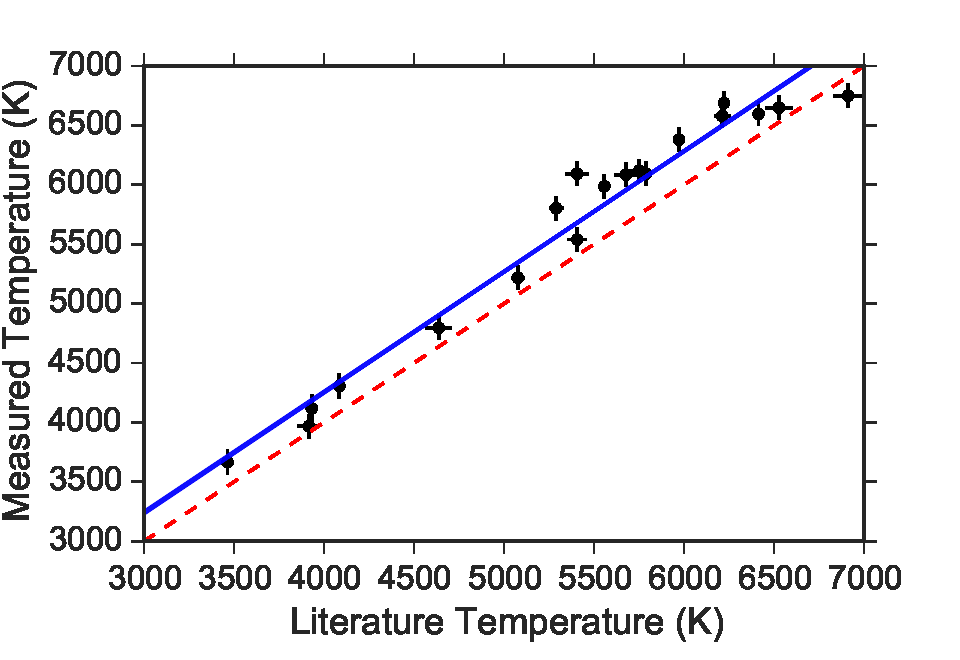
\includegraphics[scale=0.45]{Figures/paper5_TS23_simple_Tact2Tmeas.pdf}
         }%
         \subfigure[HRS]{
             \label{paper5_fig:error:b}
             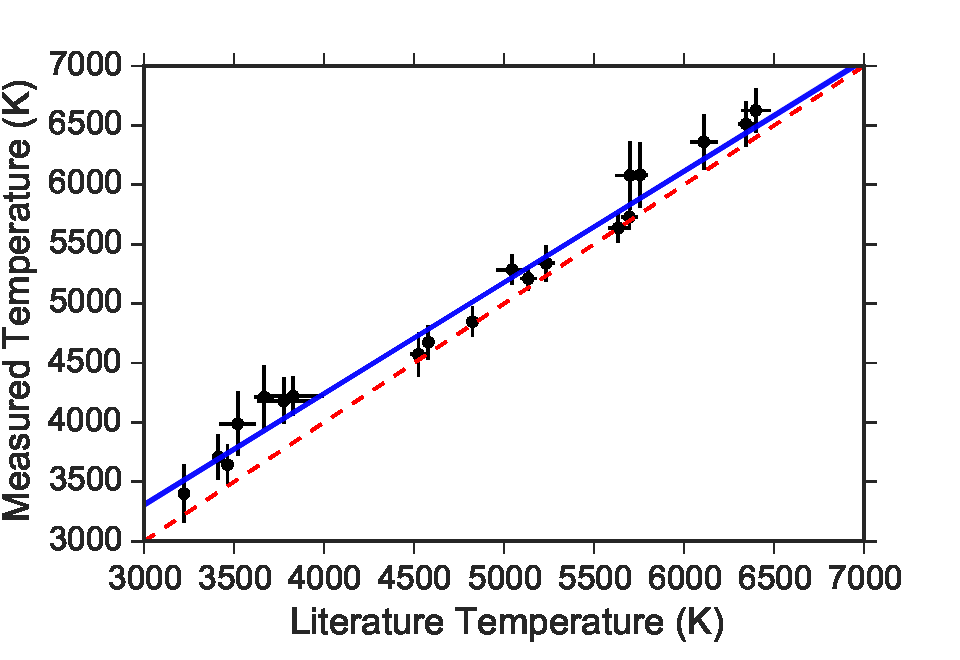
\includegraphics[scale=0.45]{Figures/paper5_HET_simple_Tact2Tmeas.pdf}
         }
         \subfigure[IGRINS]{
             \label{paper5_fig:error:c}
             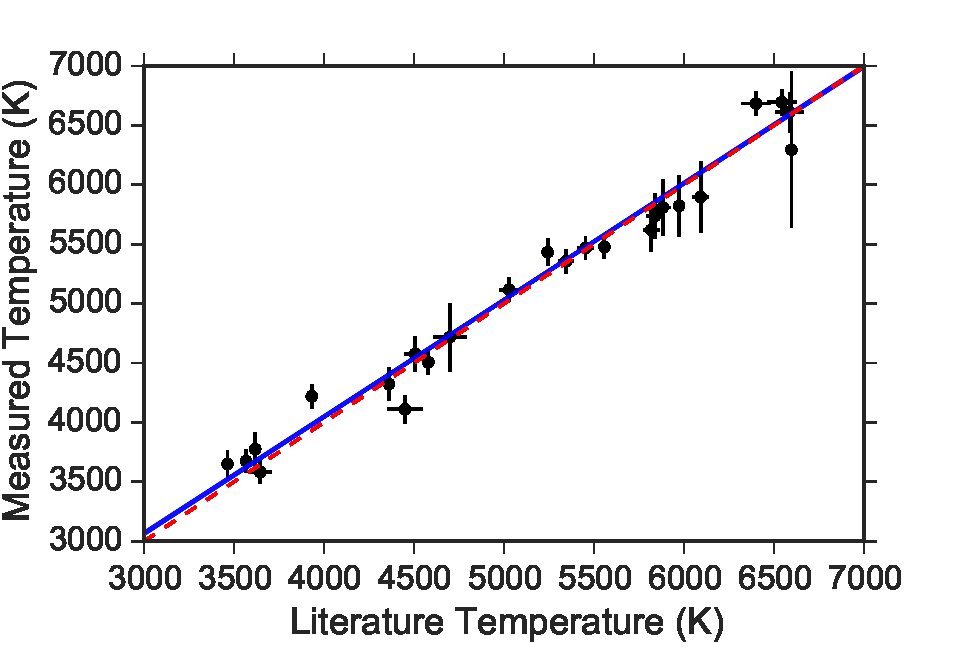
\includegraphics[scale=0.45]{Figures/paper5_IGRINS_simple_Tact2Tmeas.pdf}
         }%
         \subfigure[CHIRON]{
             \label{paper5_fig:error:d}
             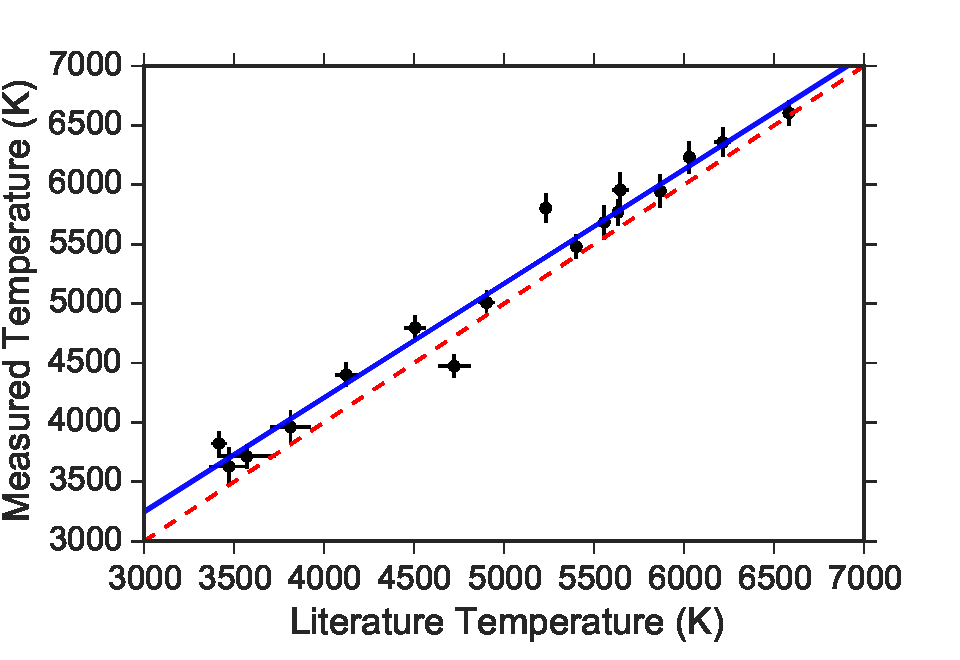
\includegraphics[scale=0.45]{Figures/paper5_CHIRON_simple_Tact2Tmeas.pdf}
         }
         \caption{Correspondence between the companion temperature measured with the direct spectral detection method, and the actual (literature) values. In all figures, the red dashed line has unity slope, the values with uncertainties are the measurements from the synthetic binary observations (see Section \ref{subpaper5_sec:systematics}), and the blue lines are the line of best-fit through the data. There is significant bias in all of the measurements except for those using the near-infrared IGRINS instrument.}
         \label{paper5_fig:error}
\end{figure}

\section{Parameter Determination}
\label{subpaper5_sec:systematics}



In the absence of noise, the CCF of an observed spectrum with a perfect model will have a value of 1 at the radial velocity of the star. As the model becomes a worse representation of the data, the peak height of the resulting CCF will decrease. Thus the CCFs act in a similar way as a $\chi^2$ map of the parameter space, allowing us to measure the effective temperature, metallicity, and rotational broadening of the secondary star. However, the presence of noise and the imperfections in the model spectra cause the measured values to deviate from the true parameters of the secondary star. 

To measure the impact of both random and systematic noise on the parameter estimation, we created several hundred synthetic binary systems for each instrument used in our program. We made the synthetic binary systems by combining the early-type star spectra from Table \ref{paper5_tab:earlycal} with those of the late-type stars in Table \ref{paper5_tab:latecal} in every possible combination, provided both observations came from the same instrument. By combining actual observations of early-type and late-type stars, our synthetic binary observations retain any instrument-specific effects that may impact the temperature estimation. We scaled the flux of the late-type star such that the flux ratio ($F_\mathrm{secondary}/F_\mathrm{primary}$) is ten times larger than the expected flux ratio for main sequence components. The artificial brightening relative to a real binary system is to ensure that the temperature estimation uncertainties are separate from the overall sensitivity of the method, which we discuss in Section \ref{subpaper5_sec:sensitivity}. We estimate the main sequence flux ratio from the published temperature of the late type star (given in Table \ref{paper5_tab:latecal}) and the published spectral types of the primaries available on Simbad \citep{Simbad}, and convert to temperature and luminosity by using Table 5 of \citet{Pecaut2013}.


We analyzed each synthetic binary star system using the method described above, and measured the temperature ($T_m$) and variance ($\sigma_T^2$) as a weighted sum near the grid point with the highest CCF peak value, weighting by the peak CCF height at each temperature ($C_i$):

\begin{eqnarray}
\label{paper5_eqn:tmeas} 
T_m &=& \sum_i C_i T_i / \sum_i C_i \\
\sigma_T^2 &=& \frac{\sum_i C_i (T_i - T_m)^2}{ \sum_i C_i - \sum_i C_i^2 / \sum_i C_i}
\end{eqnarray}

Each synthetic binary observation contributes a pair of measured and actual (literature) companion temperatures, and so each late-type star in Table \ref{paper5_tab:latecal} has many independent temperature measurements made with the DSD method. To determine the correspondence between measured and actual temperature, we perform a Markov Chain Monte Carlo (MCMC) fit to a straight line using the emcee code \citep{emcee}. We plot the mean and standard deviation of the measured temperatures in Figure \ref{paper5_fig:error}, along with 300 MCMC samples for the linear fit and the line of unity slope. The MCMC samples give posterior probability distributions for the parameters $a$ and $b$ relating the actual temperature ($T_a$) to the measured temperature ($T_m$) through

\begin{equation}
T_m = a + bT_a
\end{equation}
In Section \ref{paper5_sec:results} we invert this relation to determine the actual companion temperature, given the measured temperature from Equation \ref{paper5_eqn:tmeas}.

The typical temperature uncertainty with the DSD method is $\sim 150 - 200$ K, but the optical instruments systematically overestimate the companion temperature. \emph{The error analysis is therefore not just important to measure the parameter uncertainties, but also to get the correct answer.} We suspect the systematic biases come from a mismatch between the Phoenix model spectrum template and the real spectrum of a late-type star. The biases are different for each instrument because the instruments have different wavelength ranges, and so the spectral lines that contribute most to the cross-correlation function are different. 



\section{Detection Sensitivity}
\label{subpaper5_sec:sensitivity}



\begin{figure}[t]
  \centering
  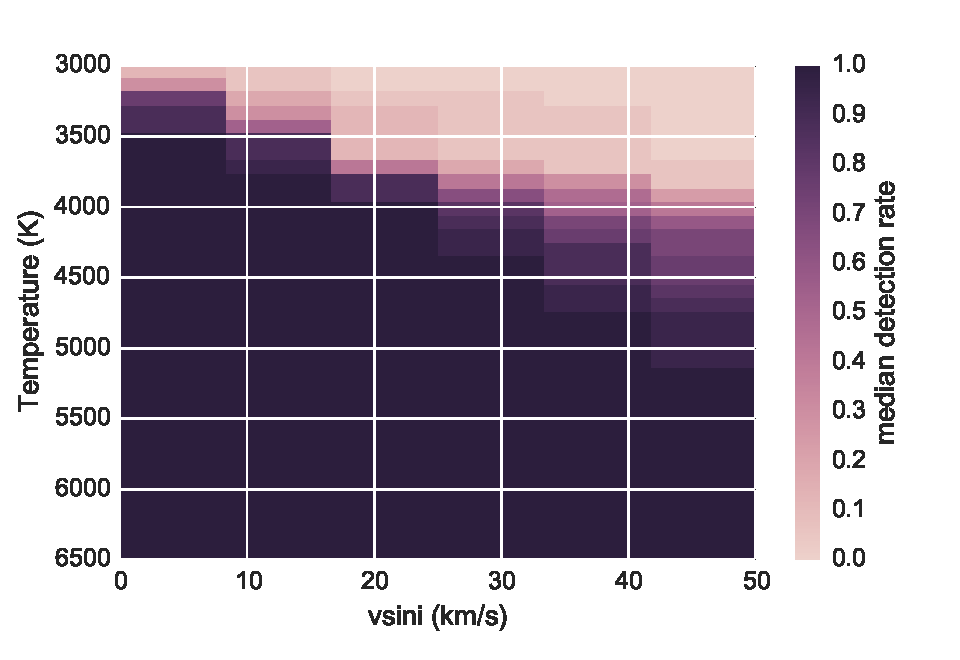
\includegraphics[width=\columnwidth]{Figures/paper5_vsini_temperature_detection_rate_median.pdf}
  \caption{Median detection rate as a function of companion temperature and rotation speed. Each cell represents the median detection rate for targets with no detection in Table \ref{paper5_tab:known}. Companions represented by dark cells are detectable. See Section \ref{subpaper5_sec:sensitivity} for details of the analysis.}
  \label{paper5_fig:sensitivity_2d}
\end{figure}

The detectability of a companion decreases primarily as the contrast between it and the primary star increases. Rotation plays an important role in the detection rate as well, since the cross-correlation function derives most of its power from narrow spectral features. We follow a similar strategy as above to estimate the detection rate as a function of temperature and rotational velocity for each star, with the key differences that we scale the model spectra to replicate a binary star observation with main sequence observations (rather than scaling the companion to ten times main sequence), and that we add \emph{Phoenix model spectra} for late-type stars to the data instead of real spectra. We use synthetic spectra so that we can use a finer grid of temperatures and rotational broadening and not be limited by the temperatures or the temperature estimation uncertainties of real late-type stars. However, since we are comparing models to models any mismatch between the model spectrum and the real spectrum of a star of that temperature will tend to make the sensitivity calculations somewhat optimistic. This will have the largest impact for very cool stars, where the difficult to model molecular absorption is more important.

For each observed early-type star, we generate several synthetic binary star observations by adding model spectra for stars with $T_\mathrm{eff} = 3000 - 7000$ K in steps of 100 K and rotational velocities $v\sin{i} = 0 - 50$ $\mathrm{km\ s}^{-1}$ in steps of 10 $\mathrm{km\ s}^{-1}$. For each temperature and $v\sin{i}$ combination, we make 17 independent synthetic observations by adding the model to the data with a radial velocity shift between -400 to 400 $\mathrm{km\ s}^{-1}$ in steps of 50 $\mathrm{km\ s}^{-1}$. We label a companion as detected if the highest peak in the CCF of the synthetic data with the model spectrum of the same temperature is within 5 $\mathrm{km\ s}^{-1}$ (the approximate instrumental broadening) of the correct velocity. 

The median detection rate for targets in Table \ref{paper5_tab:known} is shown in Figure \ref{paper5_fig:sensitivity_2d}\footnote{A file with the results of the sensitivity analysis, as well as sensitivity figures similar to Figure \ref{paper5_fig:sensitivity_2d} for each individual target, are available at this url: \url{https://github.com/kgullikson88/DSD-Paper}}. We can usually detect very cool stars if they are slowly rotating, but the sensitivity quickly degrades as the companion $v\sin{i}$ increases. Cool stars spin down as they age \citep{Barnes2003} so the rotation speed dependence is equivalent to an age dependence. We estimate the impact of rotation on our detection method by using the gyrochronology relation given in \cite{Barnes2010b}: 

\begin{equation}
\frac{k_Ct}{\tau} = \ln\left ( \frac{P}{P_0} \right ) \frac{k_Ik_C}{2\tau^2} (P^2 - P_0^2)
\label{paper5_eqn:gyro}
\end{equation}

In Equation \ref{paper5_eqn:gyro}, $k_C$ and $k_I$ are constants fit to data with known ages and rotation periods, $P$ and $P_0$ are respectively the current and zero-age main sequence (ZAMS) rotation periods, $\tau$ is the convective turnover time scale and $t$ is the current age of the star. We use the same values that \cite{Barnes2010b} use for the constants:

\begin{itemize}
\item $k_C = 0.646$ day/Myr
\item $k_I = 452$ Myr/day
\end{itemize}

We use Equation \ref{paper5_eqn:gyro} to estimate the expected rotation period for a companion star of given temperature and age as follows: First, we convert from temperature to convective timescale ($\tau$) by interpolating Table 1 in \citet{Barnes2010a}. Next we sample an appropriate probability density function (PDF) for the age of the binary system; if the primary star was analyzed in \citet{David2015}, we use their posterior age PDFs. Otherwise, we use a uniform PDF from the Zero Age Main Sequence (ZAMS) age of the primary star to its main sequence lifetime (typically 10-200 Myr for our sample). Following the discussion in \cite{Barnes2010b}, we uniformly sample initial rotation periods from 0.2 - 5 days for all stars. We estimate the current rotation period for each pair of age and initial rotation period samples using Equation \ref{paper5_eqn:gyro} to build up a PDF of current rotation periods. We transform the period distribution into a PDF for $v\sin{i}$ using the main sequence radius of a star of the given temperature, obtained by interpolating Table 1 of \cite{Barnes2010a}, and a uniform sampling of inclinations ($\sin{i}$). Figure \ref{paper5_fig:vsini} shows a typical $v\sin{i}$ distribution, which peaks near $\sim 5-10$ $\mathrm{km\ s}^{-1}$ and has a long tail extending to $\sim 40-50 \ \mathrm{km\ s}^{-1}$.


\begin{figure}[t]
    \centering
    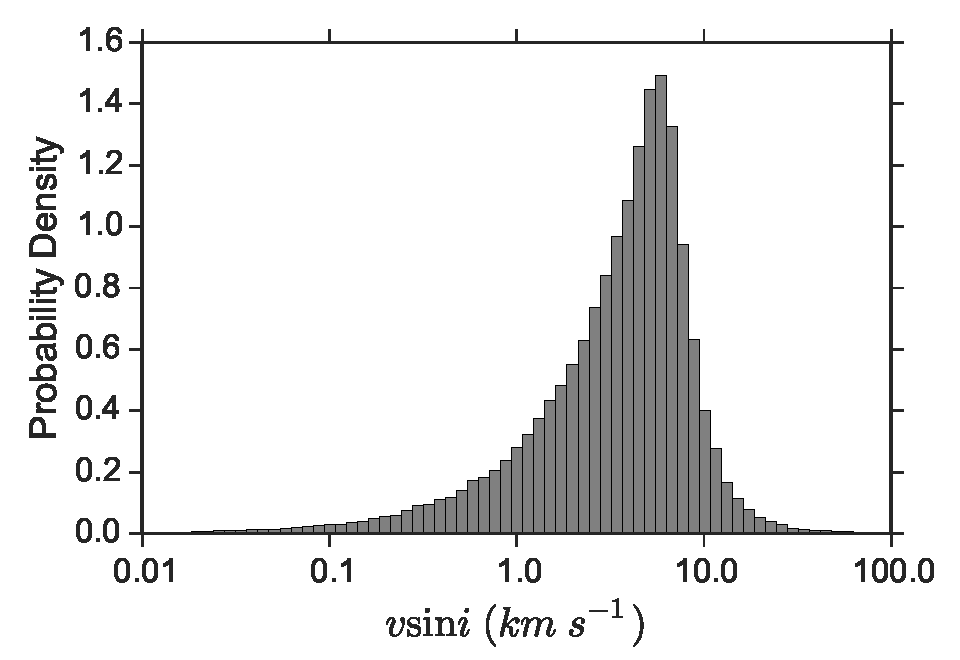
\includegraphics[width=80mm]{Figures/paper5_vsini_PDF.pdf}
    \caption{Typical probability density function for companion rotational velocity $v\sin{i}$. The distribution peaks near $\sim 5-10$ $\mathrm{km\ s}^{-1}$ and extends to very high velocities. Note that the x-axis is log-spaced to more clearly show the tails of the distribution.}
    \label{paper5_fig:vsini}
\end{figure}

By combining the sensitivity calculations described above with the $v\sin{i}$ samples, we marginalize over the expected rotation periods of the secondary stars to get simpler curves of detection rate as a function of companion star temperature. We show the median and approximate range of the marginalized detection rate in Figure \ref{paper5_fig:sensitivity}. The DSD method can reliably detect companions as cool as 3700 K in most cases, although the primary star spectral type plays a dominant role in setting the coolest detectable companion. 

Companions with $T \gtrsim 6250$ K, the canonical limit at which the convective zone is too small to transfer angular momentum to the stellar wind and spin down the star \citep{Pinsonneault2001}, may have rotational velocities comparable to that of the primary star. In that case, estimating the primary star spectrum with a gaussian filter may remove much or all of the companion spectrum. Since these are the types of stars with less extreme flux- and mass-ratios, they are easier to detect with more conventional methods. However, this shortcoming could be overcome by using model spectra for the primary star as in \citet{Kolbl2015}. In this work, we have optimized the method for finding cool companions.


\begin{figure}[t]
        \centering
        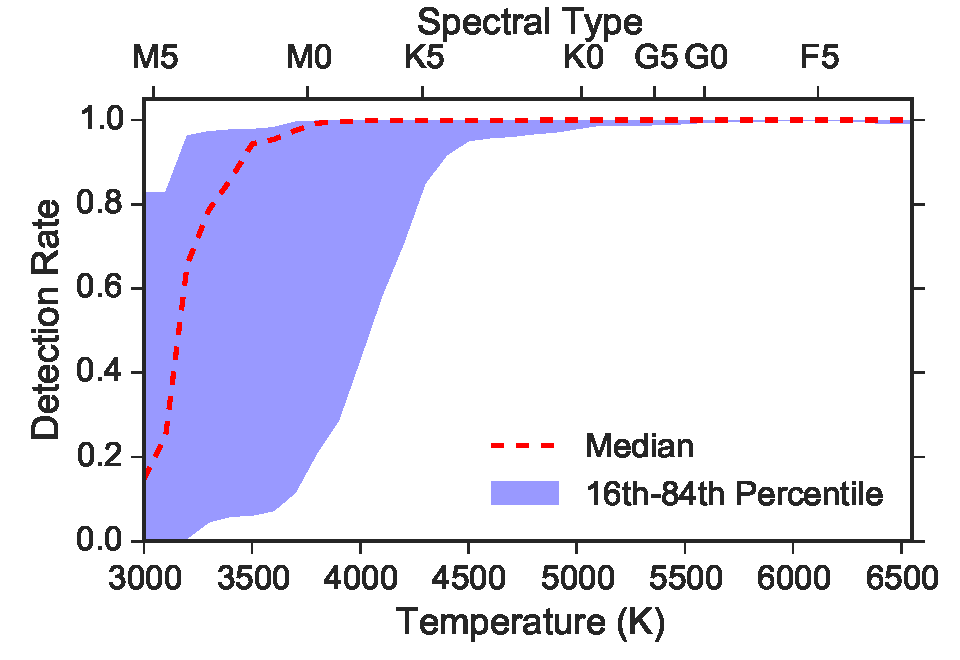
\includegraphics[width=80mm]{Figures/paper5_DetectionRate.pdf}

         \caption{Summary of the detection rate as a function of temperature for the sample stars (Table \ref{paper5_tab:known}) in which we do not detect a companion. The red dashed line gives the median detection rate, and the blue filled area illustrates the range across different primary stars. The direct spectral detection method can detect companions as late as M0 for most of our targets.}
         \label{paper5_fig:sensitivity}
\end{figure}





\begin{figure}[t]
  \centering
  \subfigure[]{
       \label{paper5_fig:detections:a}
       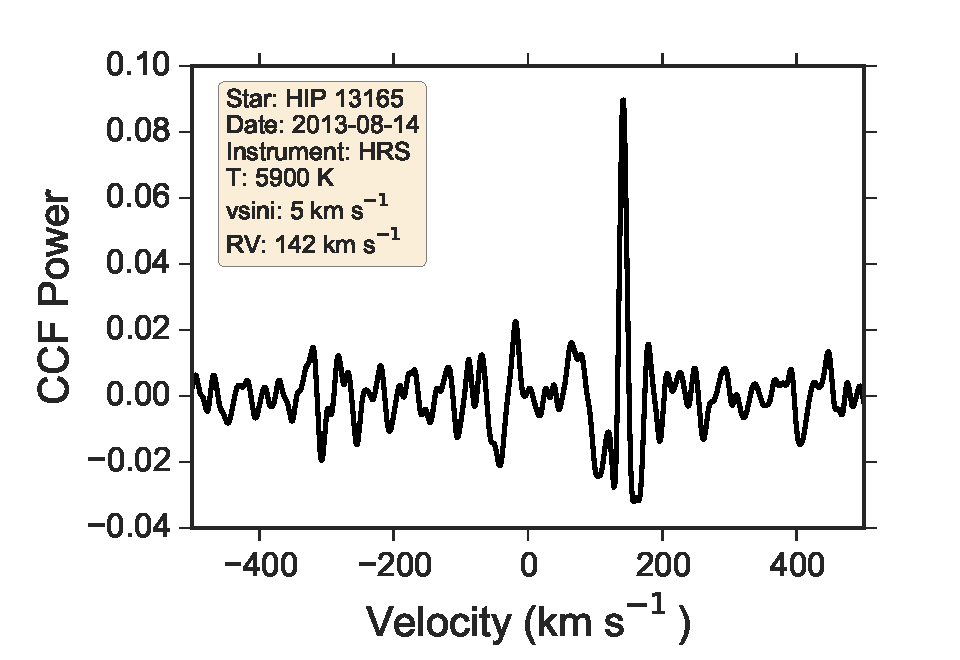
\includegraphics[width= 75mm]{Figures/paper5_HIP_13165+2013-08-14.pdf}
  }%
  \subfigure[]{
       \label{paper5_fig:detections:b}
       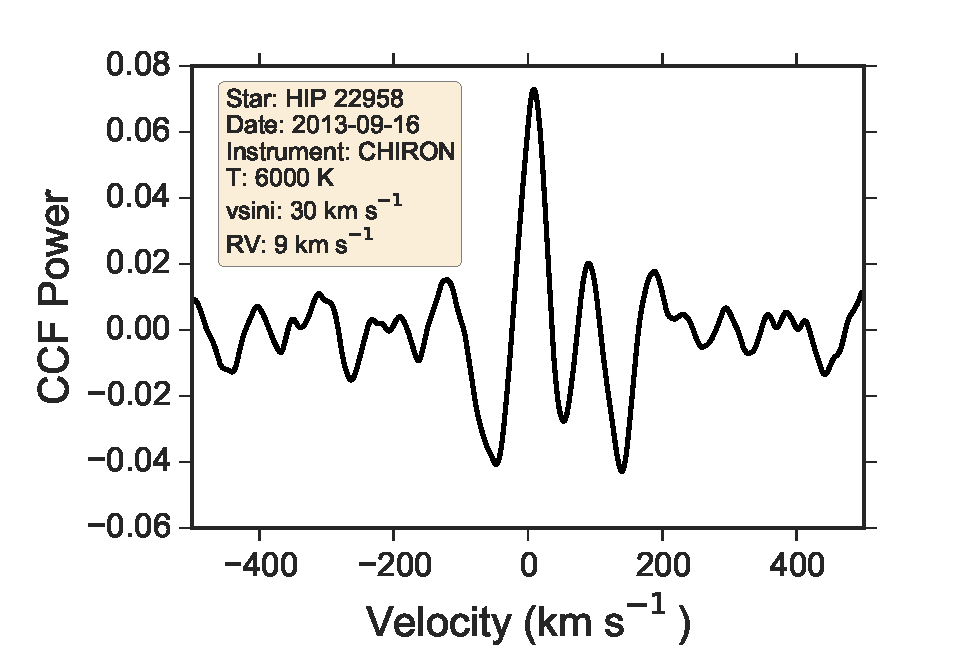
\includegraphics[width= 75mm]{Figures/paper5_HIP_22958+2013-09-16.pdf}
  }
  
  \subfigure[]{
       \label{paper5_fig:detections:c}
       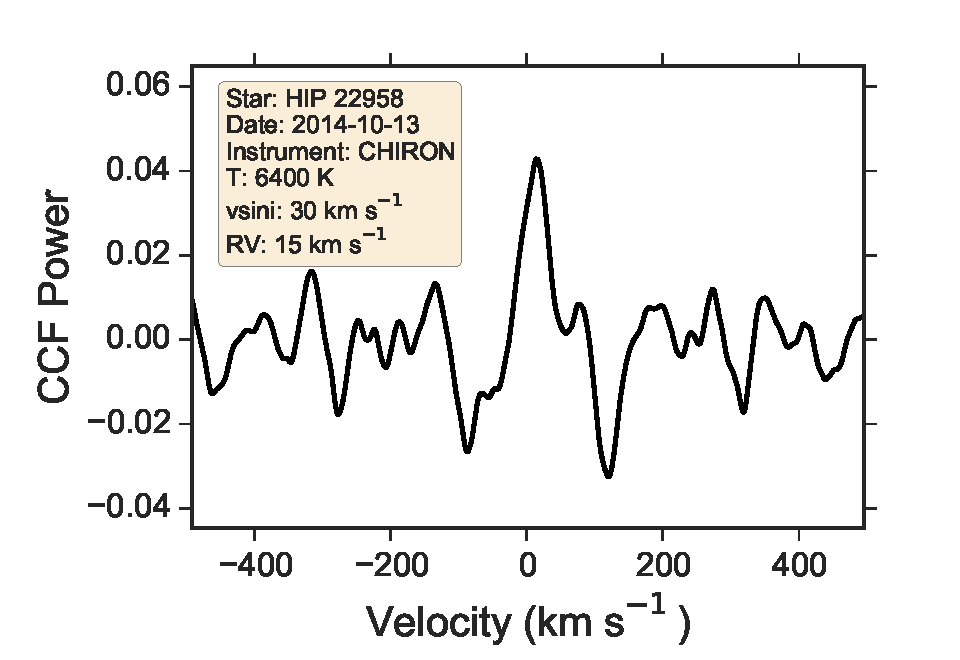
\includegraphics[width= 75mm]{Figures/paper5_HIP_22958+2014-10-13.pdf}
  }%
  \subfigure[]{
       \label{paper5_fig:detections:d}
       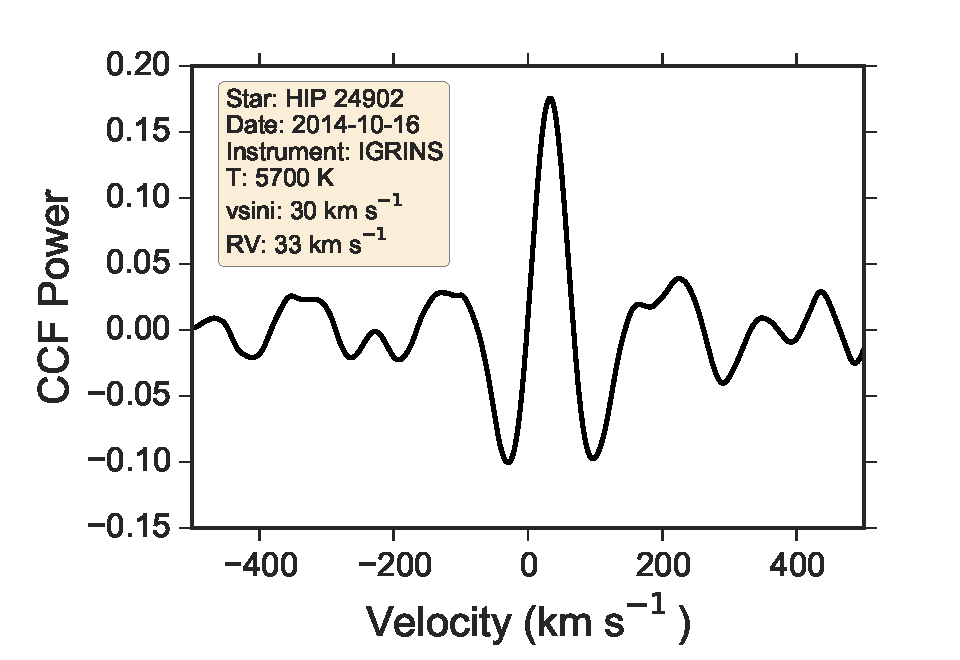
\includegraphics[width= 75mm]{Figures/paper5_HIP_24902+2014-10-16.pdf}
  }
  
  \subfigure[]{
       \label{paper5_fig:detections:e}
        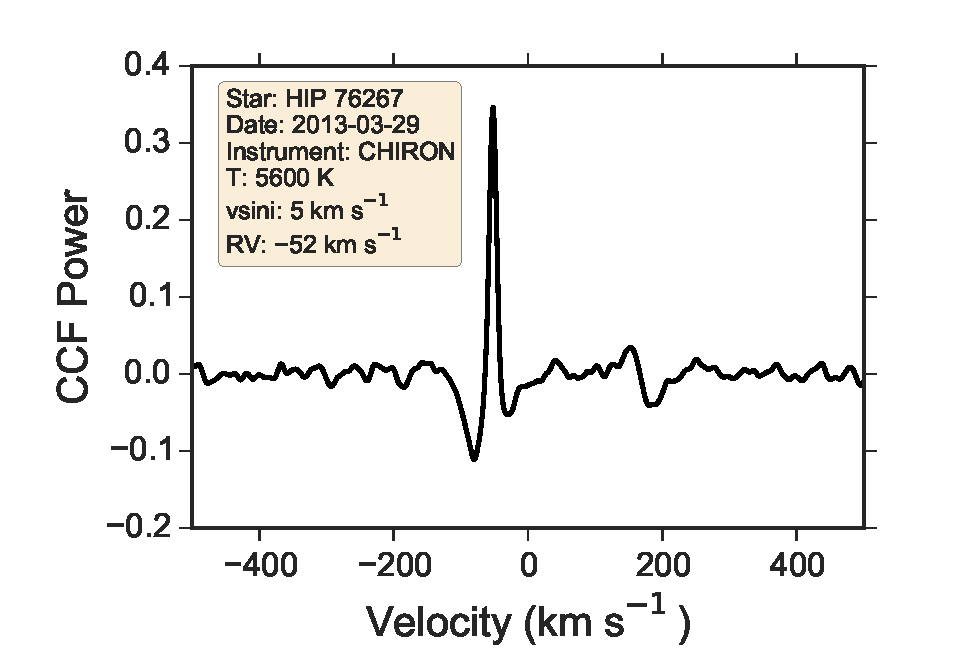
\includegraphics[width= 75mm]{Figures/paper5_HIP_76267+2013-03-29.pdf}
  }
  
  \caption{Cross-correlation functions for detected companions}
  \label{paper5_fig:detections}
\end{figure}

\begin{figure}[t]
 \centering
 
  \subfigure[]{
       \label{paper5_fig:detections2:a}
       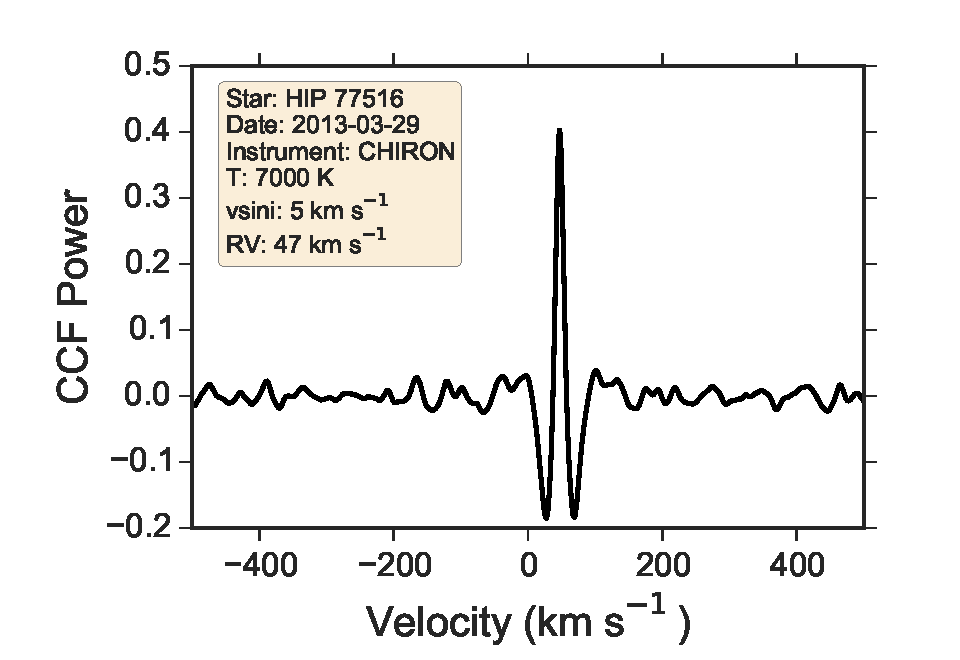
\includegraphics[width= 75mm]{Figures/paper5_HIP_77516+2013-03-29.pdf}
  }%
   \subfigure[]{
       \label{paper5_fig:detections2:b}
       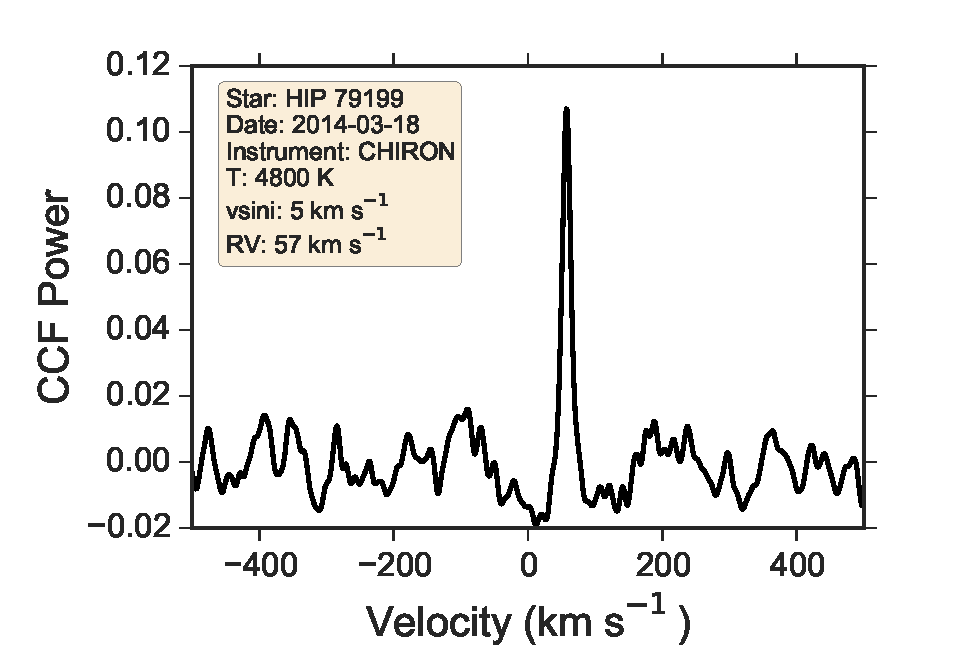
\includegraphics[width= 75mm]{Figures/paper5_HIP_79199+2014-03-18.pdf}
  }
   
  \subfigure[]{
       \label{paper5_fig:detections2:c}
       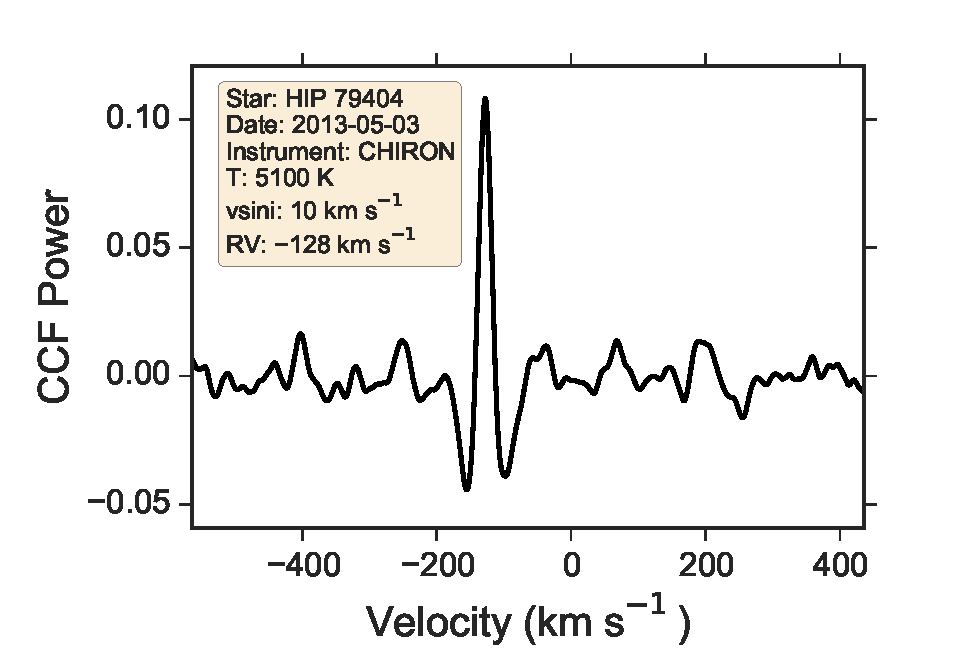
\includegraphics[width= 75mm]{Figures/paper5_HIP_79404+2013-05-03.pdf}
  }%
   \subfigure[]{
       \label{paper5_fig:detections2:d}
       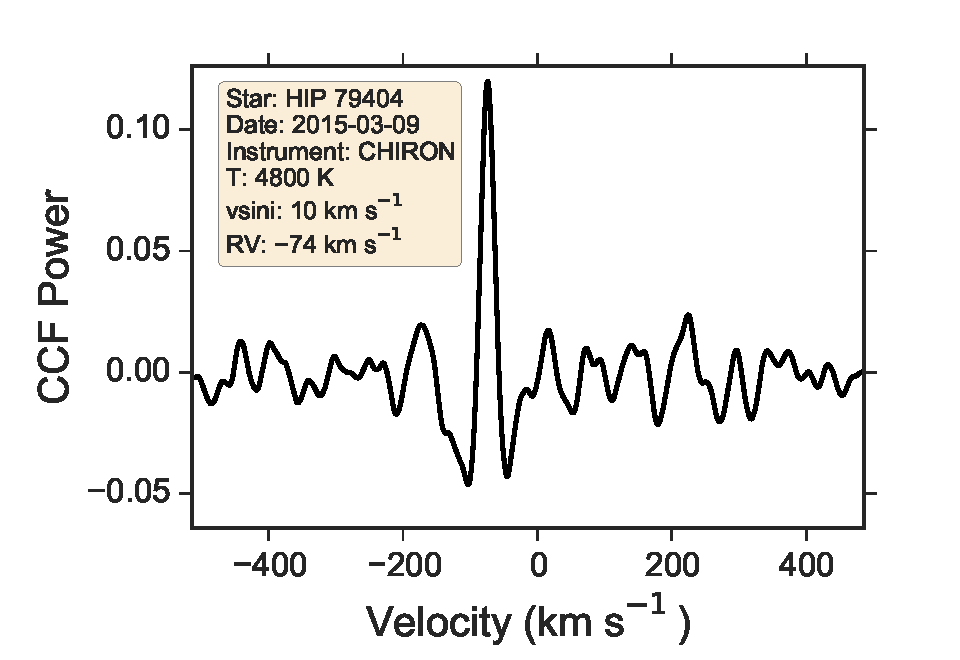
\includegraphics[width= 75mm]{Figures/paper5_HIP_79404+2015-03-09.pdf}
  }
  
  \subfigure[]{
       \label{paper5_fig:detections2:e}
       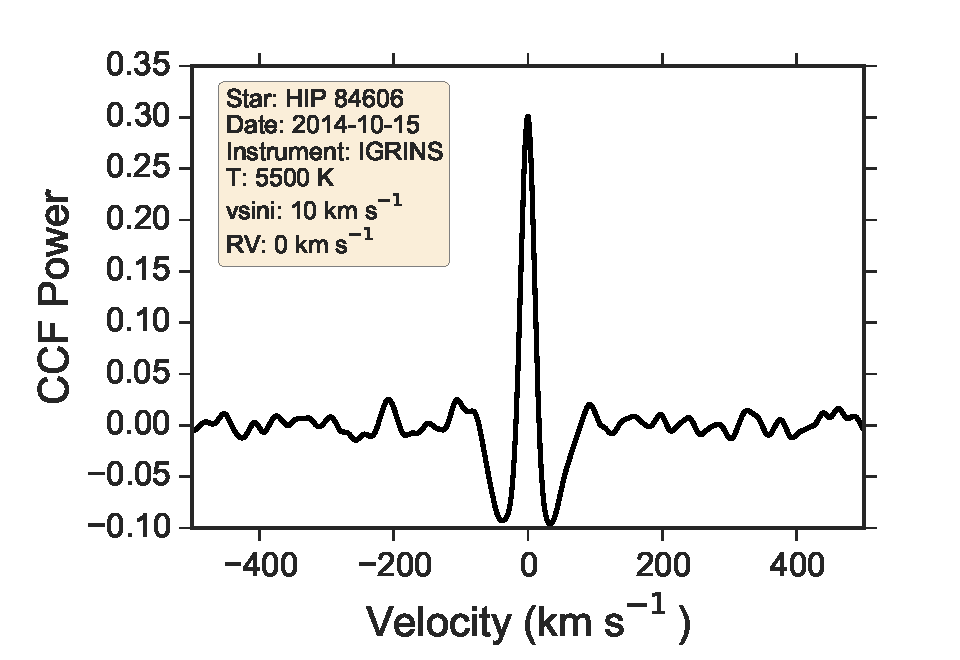
\includegraphics[width= 75mm]{Figures/paper5_HIP_84606+2014-10-15.pdf}
  }% 
  \subfigure[]{
       \label{paper5_fig:detections2:f}
       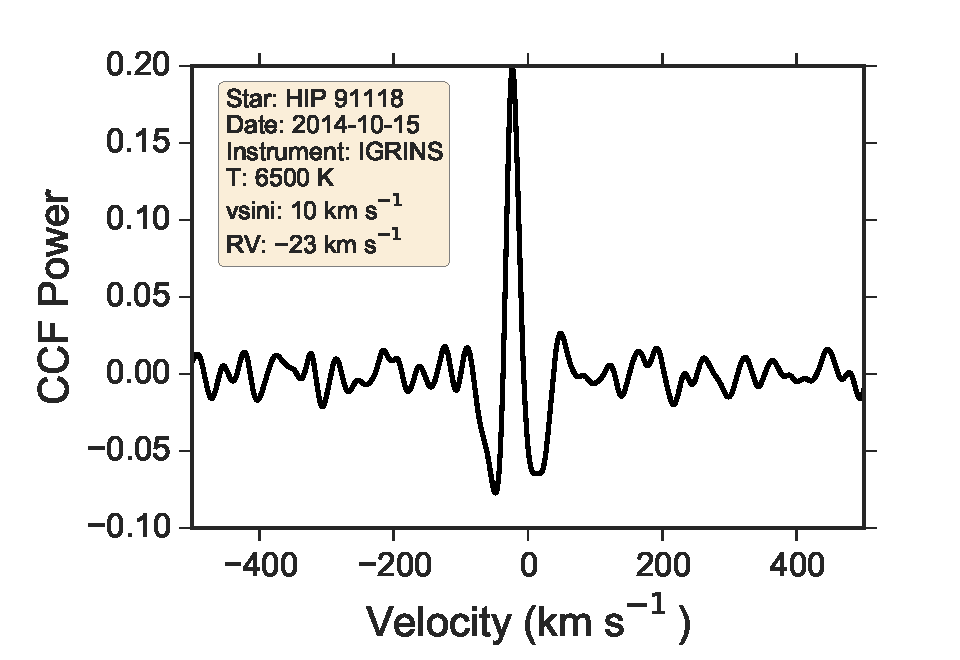
\includegraphics[width= 75mm]{Figures/paper5_HIP_91118+2014-10-15.pdf}
  } 
  
  \caption{Cross-correlation functions for detected companions}
  \label{paper5_fig:detections2}
\end{figure}

\section{Application to Known Binary Systems}
\label{paper5_sec:results}

We now use the DSD method to measure the temperatures of several known binary systems (Table \ref{paper5_tab:known}). We cross-correlate the spectra against the full grid of model spectra enumerated in Section \ref{paper5_sec:method}, and find the temperature of the companion using Equation \ref{paper5_eqn:tmeas}. We then convert the measured temperature to PDFs of the true companion temperature using the MCMC chains developed in Section \ref{subpaper5_sec:systematics} (see also Figure \ref{paper5_fig:error}). For stars with multiple observations, we multiply the PDFs from each detection. Finally, we calculate the companion temperature and confidence interval from the integral of the PDF:

\begin{equation}
f = \int_{-\infty}^x {pdf(T)dT}
\end{equation}
We use as the central value the value of x such that $f=0.5$ (the median). Likewise, we calculate the $1 \sigma$ lower and upper bounds such that $f = 0.16$ and $f = 0.84$, respectively. The CCFs for the companions that we detect are shown in Figures \ref{paper5_fig:detections} and \ref{paper5_fig:detections2}. For each star, we show the CCF which has the maximum peak value and annotate the figures with the parameters. Most of the CCFs have very strong peaks. The exception is HIP 22958; however, the detection is strengthened by the fact that we observed this star twice and measured a similar temperature both times. The CCFs for HIP 22958 and HIP 24902 demonstrate the adverse effect a large companion rotational velocity has on the detection significance.

\subsection{Comparison to Literature Data}
\label{subpaper5_sec:expected_teffs}
We use the literature data to predict an expected temperature for each companion in order to directly compare our measurements to previous results. The procedure outlined in Section \ref{paper5_sec:obs} using the magnitude difference or orbital information alone produces reasonable estimates, but in many cases there is additional information in the literature to refine the estimates. The refined estimates are described below.

HIP 76267 and HIP 84606 are found in the \cite{David2015} sample; we use the mass and temperature estimates provided there rather than going through the Simbad spectral type and assuming main-sequence relationships.

\citet{Shatsky2002} provide a color estimate of the companion star to HIP 79199 ($J-K = 0.57 \pm 0.12$). We convert this directly into a temperature estimate through Table 5 of \citet{Pecaut2013}.

\citet{Zorec2012} find fundamental parameters for HIP 22958, and determine a temperature slightly cooler and luminosity much greater than the spectral type (B6V) would suggest. Because of this the usual analysis, which uses main sequence relationships, results in a biased answer. We estimate the companion temperature by assuming that the companion \emph{does} follow the main sequence relationships as described in Section \ref{paper5_sec:obs}, but sample the uncertainty distributions given in \citet{Zorec2012} for the temperature and radius of the primary star.

We compare our companion temperature measurements from the DSD method to the estimates described above in Figure \ref{paper5_fig:known}. There is overall excellent agreement between the temperatures, with 5/6 falling within $1 \sigma$ of equality. We test for a bias ($\Delta$) between the measured temperatures ($T_m$) and expected temperatures ($T_a$) with the equations

\begin{eqnarray}
\Delta &= \sum_i(T_{m,i} - T_{a,i}) \\
\sigma_{\Delta}^2 &= \sum_i (\sigma_{T_{m,i}}^2 + \sigma_{T_{a,i}}^2)
\end{eqnarray}
which results in $\Delta = -580 \pm 770$ K. Our temperature measurements are consistent with the expected temperatures.

We list our measurements as well as the expected temperatures described above in Table \ref{paper5_tab:measured}. The expected $v\sin{i}$ values come from application of Equation \ref{paper5_eqn:gyro} as described in Section \ref{subpaper5_sec:sensitivity}. While we do give the measured $v\sin{i}$ and metallicity for our detections, the accuracy of these parameters is not calibrated and is determined with a coarse grid; the values should only be taken as rough estimates. We do note that most of the measurements have $[Fe/H] = -0.5$. This is likely a measurement bias since we do not expect the binary systems to have significantly sub-solar metallicity. As metallicity increases, so do the line depths of most of the lines in the spectrum. Any lines that are poorly modeled will then have a larger negative impact on the resulting CCF; thus the bias towards low metallicity is likely a result of imperfect model atmosphere templates. We do not attempt to identify the poorly modeled lines in this work.



\begin{figure}[t]
        \centering
        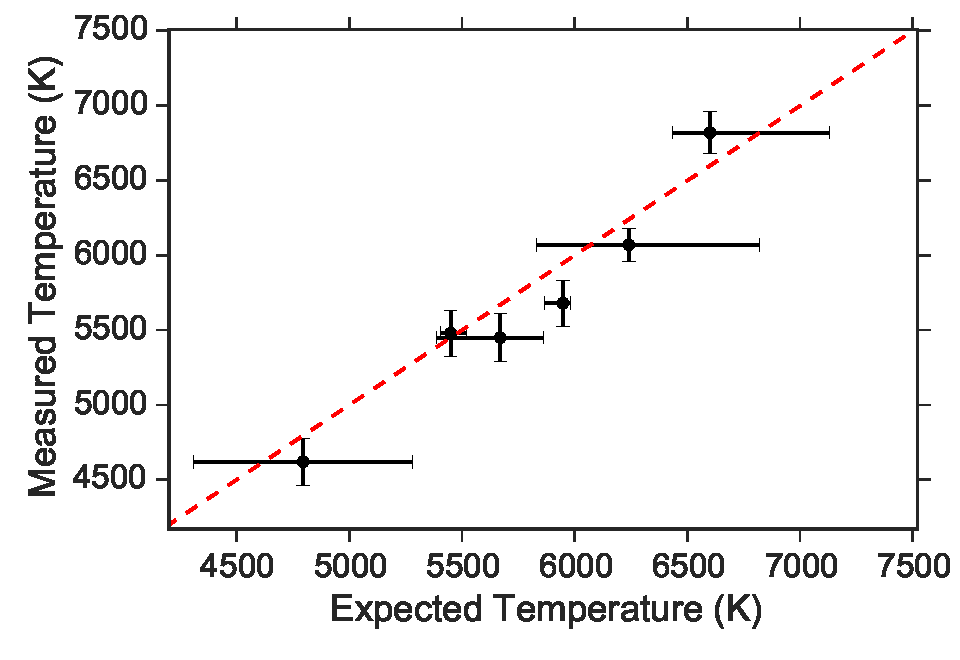
\includegraphics[width=80mm]{Figures/paper5_Known_Binaries.pdf}
        
        \caption{Temperature comparison for binaries with known secondary spectral types. The x-axis shows the companion temperature expected from the literature data (see Section \ref{subpaper5_sec:expected_teffs}).}
         \label{paper5_fig:known}
\end{figure}


\subsection{Non-detections}
\label{paper5_sec:nondetections}
There are many companions in Table \ref{paper5_tab:known} that we do not detect. Most of these are single-lined spectroscopic binaries (Table \ref{paper5_tab:specdata}), and are likely too cool to detect with our data; very high signal-to-noise spectra with a near-infrared instrument such as IGRINS may uncover them. Several of the remaining un-detected companions have expected temperatures $T  > 6250$ K, and so are likely to be rapid rotators. Since the cross-correlation function gets most of its power from  sharp spectral features, these rapidly rotating companions are difficult to detect (see Figure \ref{paper5_fig:sensitivity_2d}).  

Finally, HIP 88290 is hot enough and expected to be rotating slowly enough that we should be able to easily detect it. In fact, we would expect to be able to directly see the companion in the spectra (the green lines in Figure \ref{paper5_fig:expected}). The fact that we do not see the composite spectrum or see a peak in the cross-correlation function implies that the companion must be rotating with $v\sin{i} > 50 \mathrm{km\ s}^{-1}$, much more quickly than Equation \ref{paper5_eqn:gyro} predicts, that the primary is a giant and therefore much brighter than main-sequence relationships suggest, or that the companion fell outside the spectrograph slit. This star is in the \cite{David2015} sample and has an effective temperature and mass consistent with main sequence, so we can rule out the giant primary possibility. Additionally, the binary separation is $0.47''$ \citep{Tokovinin2015} and the CHIRON spectrograph has a $\sim 2.7''$ diameter fiber; light from the companion is guaranteed to fall on the slit.


\begin{figure}[t]
        \centering
        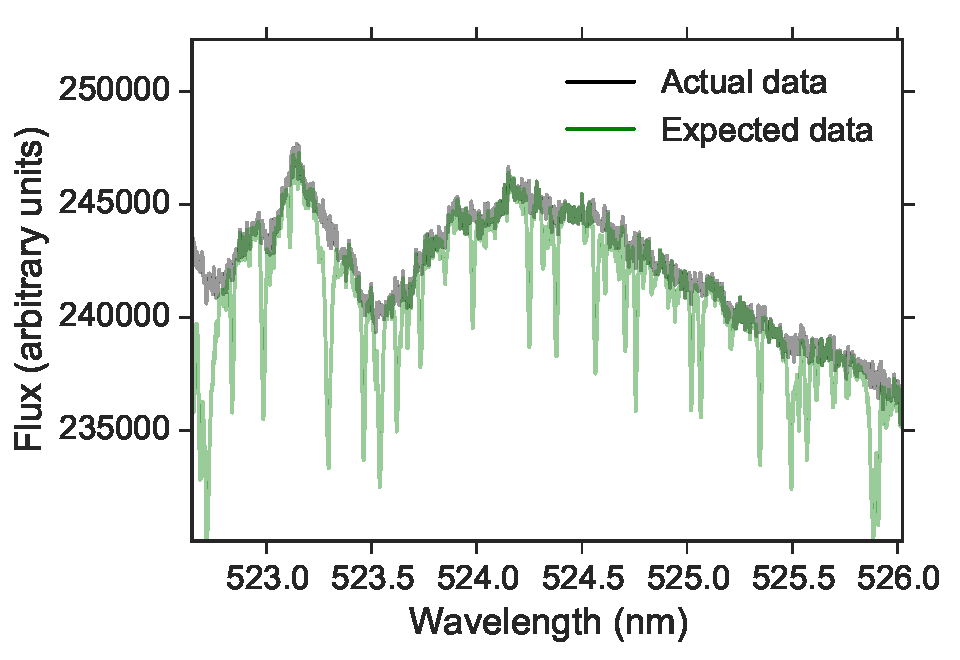
\includegraphics[width= 80mm]{Figures/paper5_HIP_88290_Flux.pdf}
         \caption{Observed (black) and expected (green) spectra for the known binary system HIP 88290. At the expected flux ratio, the spectral lines from the companion should be easily visible. }
         \label{paper5_fig:expected}
\end{figure}

\section{Discussion and Conclusions}
\label{paper5_sec:conclusions}
We have presented and extensively characterized the direct spectral detection method for finding companions to intermediate-mass stars using high-resolution cross-dispersed \'echelle spectroscopy. Using a very large number of synthetic but realistic binary star observations, we constrained the uncertainty and systematic errors present in determining the companion temperature with the direct spectral detection method. The typical uncertainties are of the order of 200 K across all instruments used in this study, with a systematic offset of similar magnitude (for the optical instruments). We used the synthetic binary star analysis to calibrate the direct spectral detection method for the four instruments used in this study between the temperatures $ 3500\ K < T < 6500\ K$.

We also estimated the sensitivity to detection of companions with a range of temperature and $v\sin{i}$ by creating a second set of synthetic companions. The method can detect companions as late as M0 in most cases, although the lower limit depends on the primary star spectral type, the signal-to-noise ratio achieved, and the instrument used. The median detection limit corresponds to average flux ratios as small as $F_\mathrm{sec}/F_\mathrm{prim} \sim 10^{-3}$ and binary mass-ratios $M_\mathrm{sec}/M_\mathrm{prim} \sim 0.2$, or a main-sequence M0 star orbiting an A0V primary.

The lowest detectable mass ratio is even more striking for young stars. At 1 Myr, both the A0 star and its companion are still contracting onto the main sequence \citep{Bressan2012}. The flux ratio limit corresponds to a $\sim$ M1 companion, similar to the main sequence case. However the mass ratio in this young system is $M_\mathrm{sec}/M_\mathrm{prim} \sim 0.1$, half that of main-sequence components with similar spectral types. The direct spectral detection method is therefore well suited for finding close, low-mass companions to massive young stars.

There is also an upper detection limit near $6500\ K$ set by rotation. Our method of removing the primary star spectrum can also remove the companion spectrum if it has a similar rotational velocity, which hot companions are likely to have. Subtracting a model atmosphere for the primary star would remove the upper limit, but would reduce the detection rate for cool companions that are most difficult to detect with any other means. We alleviate the problem somewhat in Chapter \ref{chap:survey} by extending the CCF search grid (see Section \ref{paper5_sec:method}) to higher temperatures and rotational velocities.

Finally, we applied the direct spectral detection method to a set of known binary systems with close, late-type companions. We detected the companion spectrum in 9 of 34 known binary systems, 3 of which we characterized for the first time. Most of the companions we failed to detect are likely very cool, falling below the sensitivity limit of our data.

The direct spectral detection method is able to detect close binary companions with comparable or better sensitivity than imaging techniques, and does not require large telescopes with extremely competitive time allocation requests. This method is an excellent way to identify and perform initial characterization on new binary systems using smaller telescopes, but care must be taken to calibrate the parameter estimation. 

\section*{Acknowledgements}
This research has made use of the SIMBAD database, operated at CDS, Strasbourg, France, and of Astropy, a community-developed core Python package for Astronomy (Astropy Collaboration, 2013).
It was supported by a start-up grant to Adam Kraus as well as a University of Texas Continuing Fellowship to Kevin Gullikson. J.-E. Lee was supported by the Basic Science Research Program through the National Research Foundation of Korea (NRF) (grant No. NRF-2015R1A2A2A01004769) and the Korea
Astronomy and Space Science Institute under the R\&D program (Project No. 2015-1-320-18) supervised by the Ministry of Science, ICT and Future Planning.

This work used the Immersion Grating Infrared Spectrograph (IGRINS) that was developed under a collaboration between the University of Texas at Austin and the Korea Astronomy and Space Science Institute (KASI) with the financial support of the US National Science Foundation under grant AST-1229522, of the University of Texas at Austin, and of the Korean GMT Project of KASI.

The Hobby-Eberly Telescope (HET) is a joint project of the University of Texas at Austin, the Pennsylvania State University, Stanford University, Ludwig-Maximilians-Universit\"at M\"unchen, and Georg-August-Universit\"at G\"ottingen. The HET is named in honor of its principal benefactors, William P. Hobby and Robert E. Eberly.

Based on observations at Cerro Tololo Inter-American Observatory, National Optical Astronomy Observatory (NOAO Prop. IDs: 13A-0139, 13B-0112, 2014A-0260, 14A-0260, 15A-0245; PI: Kevin Gullikson), which is operated by the Association of Universities for Research in Astronomy (AURA) under a cooperative agreement with the National Science Foundation. 

We would like to thank Bill Cochran and Mike Endl for observing some of the spectra used in this project. Finally, we would like to thank the anonymous referee for numerous comments that improved the paper.






%%%%%%%%%%%%%%%%%%%%%%%%%%%%%%%%%%%%%%%%%%%%%%%%%%
%%%%%%%              Figures                 %%%%%
%%%%%%%%%%%%%%%%%%%%%%%%%%%%%%%%%%%%%%%%%%%%%%%%%%

\clearpage
\afterpage{%
\begin{scriptsize}
\begin{longtable}{lllcccrcc}
    
    \caption{Early type star sample.\\
             The spectral types are adopted from the Simbad database \citep{Simbad}. \label{paper5_tab:earlycal}} 
    \\ \hline
     & & & & & & & & Exp. Time \\
     Star & RA & DEC & SpT & V & K & Instrument  & Date  & (min) \\ \hline
    \endfirsthead

    \caption{ - (Continued)}
    \\ \hline
    & & & & & & & & Exp. Time \\
     Star & RA & DEC & SpT & V & K & Instrument  & Date  & (min) \\ \hline
    \endhead

    \hline
    \endfoot

    \hline
    \endlastfoot

   HIP 1191 &  00:14:54.5 &  -09:34:10.4 &          B8.5V &     5.76 &     5.94 &     CHIRON &  2013-09-17 &          180.00 \\
    HIP 2381 &  00:30:22.6 &  -23:47:15.6 &            A3V &     5.19 &     4.83 &     CHIRON &  2014-08-05 &           58.18 \\
   HIP 10320 &  02:12:54.4 &  -30:43:25.7 &            B9V &     5.26 &     5.21 &     CHIRON &  2013-08-28 &          119.00 \\
   HIP 13717 &  02:56:37.4 &  -03:42:44.3 &            A3V &     5.16 &     4.86 &     CHIRON &  2014-11-09 &           74.99 \\
   HIP 14293 &  03:04:16.5 &  -07:36:03.0 &            A5V &     5.30 &     4.74 &     CHIRON &  2014-09-19 &           53.33 \\
   HIP 16285 &  03:29:55.1 &  -42:38:03.3 &            A5V &     5.77 &     5.18 &     CHIRON &  2014-10-03 &           76.29 \\
   HIP 17457 &  03:44:30.5 &  -01:09:47.1 &           B7IV &     5.25 &     5.43 &     CHIRON &  2013-08-27 &          107.13 \\
   HIP 18788 &  04:01:32.0 &  -01:32:58.7 &            B5V &     5.28 &     5.66 &     CHIRON &  2013-08-31 &          121.22 \\
   HIP 20264 &  04:20:39.0 &  -20:38:22.6 &            A0V &     5.38 &     5.33 &     CHIRON &  2014-03-02 &          100.33 \\
   HIP 20507 &  04:23:40.8 &  -03:44:43.6 &            A2V &     5.17 &     4.93 &     CHIRON &  2014-03-02 &           11.92 \\
   HIP 20507 &  04:23:40.8 &  -03:44:43.6 &            A2V &     5.17 &     4.93 &     CHIRON &  2014-03-03 &           52.30 \\
   HIP 22913 &  04:55:50.1 &  +15:02:25.0 &            B9V &     5.78 &     5.97 &     CHIRON &  2013-10-20 &          200.00 \\
   HIP 23362 &  05:01:25.5 &  -20:03:06.9 &            B9V &     4.89 &     4.97 &     CHIRON &  2013-09-13 &           84.58 \\
   HIP 25280 &  05:24:28.4 &  -16:58:32.8 &            A0V &     5.64 &     5.65 &     CHIRON &  2014-10-20 &           67.52 \\
   HIP 25608 &  05:28:15.3 &  -37:13:50.7 &            A1V &     5.56 &     5.50 &     CHIRON &  2014-03-02 &          103.00 \\
   HIP 27321 &  05:47:17.0 &  -51:03:59.4 &            A6V &     3.86 &     3.48 &     CHIRON &  2014-02-08 &           23.23 \\
   HIP 28910 &  06:06:09.3 &  -14:56:06.9 &            A0V &     4.67 &     4.52 &     CHIRON &  2014-02-05 &           33.31 \\
   HIP 29735 &  06:15:44.8 &  -13:43:06.2 &            B9V &     5.00 &     5.10 &     CHIRON &  2013-09-24 &           93.68 \\
   HIP 30069 &  06:19:40.9 &  -34:23:47.7 &            B9V &     5.75 &     5.93 &     CHIRON &  2013-10-08 &          180.00 \\
   HIP 30788 &  06:28:10.2 &  -32:34:48.2 &            B4V &     4.48 &     4.91 &     CHIRON &  2013-10-09 &           56.93 \\
   HIP 31362 &  06:34:35.3 &  -32:42:58.5 &            B8V &     5.61 &     5.73 &     CHIRON &  2013-11-02 &          160.00 \\
   HIP 32474 &  06:46:39.0 &  -10:06:26.4 &          B9.5V &     5.65 &     5.66 &     CHIRON &  2013-10-27 &          160.00 \\
   HIP 33575 &  06:58:35.8 &  -25:24:50.9 &            B2V &     5.58 &     6.05 &     CHIRON &  2013-11-03 &          140.00 \\
   HIP 35180 &  07:16:14.5 &  -15:35:08.4 &            A1V &     5.45 &     5.27 &     CHIRON &  2014-02-08 &           90.55 \\
     HR 2948 &  07:38:49.3 &  -26:48:06.4 &            B6V &     4.50 &     4.96 &     CHIRON &  2013-10-19 &           67.20 \\
   HIP 37450 &  07:41:15.8 &  -38:32:00.7 &            B5V &     5.41 &     5.78 &     CHIRON &  2013-11-04 &          136.62 \\
   HIP 40429 &  08:15:15.9 &  -62:54:56.3 &            A2V &     5.16 &  \nodata &     CHIRON &  2014-02-03 &           82.83 \\
   HIP 40706 &  08:18:33.3 &  -36:39:33.4 &            A8V &     4.40 &     4.00 &     CHIRON &  2013-02-04 &           32.32 \\
   HIP 42334 &  08:37:52.1 &  -26:15:18.0 &            A0V &     5.27 &     5.32 &     CHIRON &  2014-02-24 &           48.60 \\
   HIP 45344 &  09:14:24.4 &  -43:13:38.9 &            B4V &     5.25 &     5.59 &     CHIRON &  2013-11-16 &          116.78 \\
     HR 4259 &  10:55:36.8 &  +24:44:59.0 &            A1V &     4.50 &  \nodata &     CHIRON &  2013-02-12 &           35.47 \\
   HIP 56633 &  11:36:40.9 &  -09:48:08.0 &         B9.5Vn &     4.68 &     4.78 &     CHIRON &  2013-02-12 &           41.77 \\
   HIP 57328 &  11:45:17.0 &  +08:15:29.2 &            A4V &     4.84 &     4.41 &     CHIRON &  2013-02-15 &           48.88 \\
   HIP 57328 &  11:45:17.0 &  +08:15:29.2 &            A4V &     4.84 &     4.41 &     CHIRON &  2013-03-19 &           48.88 \\
   HIP 61622 &  12:37:42.1 &  -48:32:28.6 &         A1IVnn &     3.86 &     3.70 &     CHIRON &  2013-03-27 &           19.48 \\
   HIP 66249 &  13:34:41.7 &  -00:35:45.3 &          A2Van &     3.38 &     3.07 &     CHIRON &  2013-03-27 &           12.83 \\
   HIP 66821 &  13:41:44.7 &  -54:33:33.9 &  B8.5Vn        &     5.01 &  \nodata &     CHIRON &  2014-03-02 &           71.17 \\
   HIP 68520 &  14:01:38.7 &  +01:32:40.3 &            A3V &     4.24 &     4.09 &     CHIRON &  2013-04-21 &           27.88 \\
   HIP 70327 &  14:23:22.6 &  +08:26:47.8 &            A0V &     5.12 &     5.07 &     CHIRON &  2014-03-03 &           42.15 \\
   HIP 72104 &  14:44:59.2 &  -35:11:30.5 &            A0V &     4.92 &     4.78 &     CHIRON &  2014-03-04 &           58.09 \\
   HIP 73049 &  14:55:44.7 &  -33:51:20.8 &            A0V &     5.32 &     5.13 &     CHIRON &  2014-02-27 &           69.75 \\
   HIP 75304 &  15:23:09.3 &  -36:51:30.5 &            B4V &     4.54 &     4.94 &     CHIRON &  2013-05-15 &           36.05 \\
   HIP 77233 &  15:46:11.2 &  +15:25:18.5 &            A3V &     3.67 &     3.42 &     CHIRON &  2013-05-14 &           16.33 \\
   HIP 77635 &  15:50:58.7 &  -25:45:04.6 &         B1.5Vn &     4.64 &     4.78 &     CHIRON &  2014-03-09 &           30.80 \\
   HIP 78105 &  15:56:53.4 &  -33:57:58.0 &            A3V &     5.08 &     4.85 &     CHIRON &  2014-07-31 &           21.30 \\
   HIP 78105 &  15:56:53.4 &  -33:57:58.0 &            A3V &     5.08 &     4.85 &     CHIRON &  2014-08-01 &           48.91 \\
   HIP 78106 &  15:56:54.1 &  -33:57:51.3 &            B9V &     5.55 &     5.42 &     CHIRON &  2014-03-20 &           70.48 \\
   HIP 78554 &  16:02:17.6 &  +22:48:16.0 &            A3V &     4.82 &     4.62 &     CHIRON &  2013-05-15 &           47.60 \\
   HIP 79007 &  16:07:37.5 &  +09:53:30.2 &            A7V &     5.64 &     5.09 &     CHIRON &  2014-08-04 &           58.79 \\
   HIP 79007 &  16:07:37.5 &  +09:53:30.2 &            A7V &     5.64 &     5.09 &     CHIRON &  2014-08-05 &           21.23 \\
   HIP 79387 &  16:12:07.3 &  -08:32:51.2 &            A4V &     5.43 &     5.05 &     CHIRON &  2014-03-30 &           70.72 \\
   HIP 79653 &  16:15:15.3 &  -47:22:19.2 &            B8V &     5.12 &     5.42 &     CHIRON &  2014-03-24 &           47.12 \\
   HIP 80815 &  16:30:12.4 &  -25:06:54.8 &            B3V &     4.79 &     5.10 &     CHIRON &  2013-03-27 &           45.85 \\
   HIP 85537 &  17:28:49.6 &  +00:19:50.2 &            A7V &     5.42 &     4.80 &     CHIRON &  2014-05-15 &           60.83 \\
   HIP 85922 &  17:33:29.8 &  -05:44:41.2 &            A5V &     5.62 &     5.14 &     CHIRON &  2014-08-17 &           95.90 \\
   HIP 86019 &  17:34:46.3 &  -11:14:31.1 &           B8Vn &     5.54 &     5.36 &     CHIRON &  2014-03-31 &           69.76 \\
   HIP 87108 &  17:47:53.5 &  +02:42:26.2 &        A1Vnk &     3.75 &     3.65 &     CHIRON &  2013-06-02 &           17.73 \\
   HIP 90887 &  18:32:21.3 &  -39:42:14.4 &           A3Vn &     5.16 &     4.93 &     CHIRON &  2014-04-01 &           73.61 \\
   HIP 91875 &  18:43:46.9 &  -38:19:24.3 &           A2Vn &     5.12 &     4.86 &     CHIRON &  2014-03-29 &           46.61 \\
   HIP 92946 &  18:56:13.1 &  +04:12:12.9 &            A5V &     4.62 &     4.09 &     CHIRON &  2013-07-02 &           39.55 \\
   HIP 93805 &  19:06:14.9 &  -04:52:57.2 &           B9Vn &     3.43 &     3.65 &     CHIRON &  2014-04-28 &           10.92 \\
  HIP 101589 &  20:35:18.5 &  +14:40:27.1 &            A3V &     4.66 &     4.36 &     CHIRON &  2013-06-05 &           41.07 \\
  HIP 104139 &  21:05:56.8 &  -17:13:58.3 &            A1V &     4.07 &     4.10 &     CHIRON &  2013-06-05 &           23.80 \\
  HIP 105140 &  21:17:56.2 &  -32:10:21.1 &            A1V &     4.72 &     4.49 &     CHIRON &  2013-07-12 &           43.40 \\
  HIP 107517 &  21:46:32.0 &  -11:21:57.4 &            A1V &     5.57 &     5.57 &     CHIRON &  2014-08-04 &          118.70 \\
  HIP 107608 &  21:47:44.1 &  -30:53:53.9 &            A2V &     5.02 &     4.85 &     CHIRON &  2014-05-11 &           52.76 \\
  HIP 108294 &  21:56:22.7 &  -37:15:13.1 &           A2Vn &     5.46 &     5.17 &     CHIRON &  2014-05-13 &           57.20 \\
  HIP 110935 &  22:28:37.6 &  -67:29:20.6 &            A4V &     5.57 &     5.05 &     CHIRON &  2014-08-27 &           74.48 \\
  HIP 117089 &  23:44:12.0 &  -18:16:36.9 &            B9V &     5.24 &     5.38 &     CHIRON &  2013-08-09 &          102.52 \\
    HIP 5361 &  01:08:33.4 &  +58:15:48.4 &            B8V &     5.77 &     5.75 &        HRS &  2013-08-19 &           50.00 \\
    HIP 8016 &  01:42:55.8 &  +70:37:21.0 &            B9V &     5.18 &     5.22 &        HRS &  2013-08-18 &           16.40 \\
   HIP 14043 &  03:00:52.2 &  +52:21:06.2 &            B7V &     5.25 &     5.43 &        HRS &  2013-08-19 &           20.00 \\
   HIP 14143 &  03:02:22.5 &  +04:21:10.3 &            B7V &     5.61 &     5.90 &        HRS &  2013-08-14 &           23.10 \\
   HIP 15404 &  03:18:37.7 &  +50:13:19.8 &            B3V &     5.16 &     5.33 &        HRS &  2013-08-13 &           10.25 \\
   HIP 18396 &  03:55:58.1 &  +47:52:17.1 &            B6V &     5.38 &     5.58 &        HRS &  2013-08-12 &           12.95 \\
   HIP 20430 &  04:22:34.9 &  +25:37:45.5 &          B9Vnn &     5.38 &     5.45 &        HRS &  2013-08-16 &           18.00 \\
   HIP 20579 &  04:24:29.1 &  +34:07:50.7 &            B8V &     5.72 &     5.81 &        HRS &  2013-08-13 &           24.50 \\
   HIP 66798 &  13:41:29.8 &  +64:49:20.6 &            A2V &     5.85 &     5.65 &        HRS &  2013-03-26 &           18.10 \\
   HIP 67194 &  13:46:13.5 &  +41:05:19.4 &            A5V &     5.89 &     5.34 &        HRS &  2013-04-07 &           18.40 \\
   HIP 67782 &  13:53:10.2 &  +28:38:53.2 &            A7V &     5.91 &     5.47 &        HRS &  2013-04-12 &           17.95 \\
   HIP 70384 &  14:24:00.8 &  +08:14:38.2 &            A3V &     5.93 &     5.72 &        HRS &  2013-04-21 &           21.00 \\
   HIP 72154 &  14:45:30.2 &  +00:43:02.1 &          B9.5V &     5.67 &     5.60 &        HRS &  2013-04-21 &           15.00 \\
   HIP 80991 &  16:32:25.6 &  +60:49:23.9 &            A2V &     5.91 &     5.78 &        HRS &  2013-04-07 &           20.20 \\
   HIP 82350 &  16:49:34.6 &  +13:15:40.1 &            A1V &     5.91 &     5.86 &        HRS &  2013-04-09 &           20.20 \\
   HIP 83635 &  17:05:32.2 &  -00:53:31.4 &            B1V &     5.61 &     5.29 &        HRS &  2013-04-25 &           15.80 \\
   HIP 85379 &  17:26:44.2 &  +48:15:36.2 &            A4V &     5.83 &     5.38 &        HRS &  2013-04-16 &           16.50 \\
   HIP 86782 &  17:43:59.1 &  +53:48:06.1 &            A2V &     5.76 &     5.59 &        HRS &  2013-04-22 &           15.50 \\
   HIP 88817 &  18:07:49.5 &  +26:05:50.4 &            A3V &     5.90 &     5.51 &        HRS &  2013-04-23 &           20.00 \\
   HIP 90052 &  18:22:35.3 &  +12:01:46.8 &            A2V &     5.98 &     5.77 &        HRS &  2013-04-23 &           25.00 \\
   HIP 92312 &  18:48:53.3 &  +19:19:43.3 &            A1V &     5.89 &     5.82 &        HRS &  2013-04-26 &           19.50 \\
   HIP 93393 &  19:01:17.3 &  +26:17:29.0 &            B5V &     5.68 &     5.84 &        HRS &  2013-04-22 &           16.00 \\
   HIP 96840 &  19:41:05.5 &  +13:48:56.4 &            B5V &     5.99 &     6.21 &        HRS &  2013-04-26 &           27.60 \\
  HIP 100069 &  20:18:06.9 &  +40:43:55.5 &            O9V &     5.84 &     5.72 &        HRS &  2013-04-27 &           22.55 \\
  HIP 105282 &  21:19:28.7 &  +49:30:37.0 &            B6V &     5.74 &     6.08 &        HRS &  2013-08-18 &           36.77 \\
  HIP 105942 &  21:27:21.3 &  +37:07:00.4 &            B3V &     5.29 &     5.64 &        HRS &  2013-08-19 &           24.00 \\
  HIP 105972 &  21:27:46.1 &  +66:48:32.7 &            B7V &     5.41 &     5.60 &        HRS &  2013-08-03 &           13.35 \\
    HIP 5132 &  01:05:41.7 &  +21:27:55.5 &           A0Vn &     5.53 &     5.61 &     IGRINS &  2014-07-09 &            6.67 \\
    HIP 5518 &  01:10:39.3 &  +68:46:43.0 &          A0Vnn &     5.32 &     5.31 &     IGRINS &  2014-10-15 &            3.73 \\
    HIP 5626 &  01:12:16.8 &  +79:40:26.2 &            A3V &     5.60 &     5.49 &     IGRINS &  2014-10-15 &            3.73 \\
    HIP 9564 &  02:02:52.4 &  +64:54:05.2 &           A1Vn &     6.00 &     5.92 &     IGRINS &  2014-10-15 &            3.73 \\
   HIP 12803 &  02:44:32.9 &  +15:18:42.7 &           B9Vn &     5.78 &     5.79 &     IGRINS &  2014-10-17 &            3.73 \\
   HIP 13879 &  02:58:45.6 &  +39:39:45.8 &           A2Vn &     4.70 &     4.42 &     IGRINS &  2014-10-15 &            3.73 \\
   HIP 14862 &  03:11:56.2 &  +74:23:37.1 &          A2Vnn &     4.84 &     4.71 &     IGRINS &  2014-10-15 &            3.73 \\
   HIP 15110 &  03:14:54.0 &  +21:02:40.0 &            A1V &     4.88 &     4.82 &     IGRINS &  2014-10-16 &            4.20 \\
   HIP 16599 &  03:33:39.0 &  +54:58:29.4 &            A3V &     5.98 &     5.68 &     IGRINS &  2014-10-15 &            3.73 \\
   HIP 17527 &  03:45:09.7 &  +24:50:21.3 &            B8V &     5.64 &     5.81 &     IGRINS &  2014-10-17 &            3.73 \\
   HIP 20789 &  04:27:17.4 &  +22:59:46.8 &            B7V &     5.51 &     5.74 &     IGRINS &  2014-10-16 &            3.73 \\
   HIP 21683 &  04:39:16.5 &  +15:55:04.7 &           A5Vn &     4.68 &     4.23 &     IGRINS &  2014-10-18 &            3.83 \\
   HIP 22028 &  04:44:07.9 &  -18:39:59.7 &            A1V &     5.53 &     5.44 &     IGRINS &  2014-10-17 &            4.00 \\
   HIP 23362 &  05:01:25.5 &  -20:03:06.9 &            B9V &     4.89 &     4.97 &     IGRINS &  2014-10-16 &            4.00 \\
 ADS 3962 AB &  05:22:50.3 &     +03 32 52 &           B1Vn &     4.99 &  \nodata &     IGRINS &  2014-10-16 &            4.67 \\
   HIP 25143 &  05:22:50.3 &  +41:01:45.3 &            A3V &     5.55 &     5.11 &     IGRINS &  2014-10-16 &            3.73 \\
   HIP 25280 &  05:24:28.4 &  -16:58:32.8 &            A0V &     5.64 &     5.65 &     IGRINS &  2014-10-17 &            4.00 \\
   HIP 25790 &  05:30:26.1 &  +15:21:37.6 &           A3Vn &     5.94 &     5.55 &     IGRINS &  2014-10-16 &            3.73 \\
   HIP 26093 &  05:33:54.2 &  +14:18:20.0 &            B3V &     5.59 &     5.96 &     IGRINS &  2014-10-16 &            4.67 \\
   HIP 27713 &  05:52:07.7 &  -09:02:30.8 &           A2Vn &     5.96 &     5.65 &     IGRINS &  2014-10-16 &            4.00 \\
   HIP 29151 &  06:08:57.9 &  +02:29:58.8 &           A3Vn &     5.73 &     5.35 &     IGRINS &  2014-10-16 &            4.40 \\
   HIP 29735 &  06:15:44.8 &  -13:43:06.2 &            B9V &     5.00 &     5.10 &     IGRINS &  2014-10-16 &            4.00 \\
   HIP 30666 &  06:26:39.5 &  -01:30:26.4 &           A3Vn &     5.87 &     5.64 &     IGRINS &  2014-10-16 &            4.67 \\
   HIP 31278 &  06:33:37.9 &  -01:13:12.5 &           B5Vn &     5.08 &     5.46 &     IGRINS &  2014-10-16 &            4.00 \\
   HIP 36812 &  07:34:15.8 &  +03:22:18.1 &          A0Vnn &     5.83 &     5.74 &     IGRINS &  2014-10-17 &            4.00 \\
   HIP 40881 &  08:20:32.1 &  +24:01:20.3 &          B9.5V &     5.93 &     5.91 &     IGRINS &  2014-10-17 &            4.00 \\
   HIP 85290 &  17:25:41.3 &  +60:02:54.2 &           A1Vn &     5.64 &     5.50 &     IGRINS &  2014-10-16 &            3.73 \\
   HIP 85385 &  17:26:49.1 &  +20:04:51.5 &            B5V &     5.51 &     5.84 &     IGRINS &  2014-07-10 &            8.00 \\
   HIP 93713 &  19:04:55.1 &  +53:23:47.9 &           A0Vn &     5.38 &     5.41 &     IGRINS &  2014-07-10 &            8.00 \\
   HIP 94620 &  19:15:17.3 &  +21:13:55.6 &            A4V &     5.65 &     5.30 &     IGRINS &  2014-07-10 &            10.00 \\
   HIP 97376 &  19:47:27.7 &  +38:24:27.4 &           B8Vn &     5.83 &     6.01 &     IGRINS &  2014-07-10 &            8.00 \\
   HIP 99742 &  20:14:16.6 &  +15:11:51.3 &            A2V &     4.95 &     4.77 &     IGRINS &  2014-10-15 &            8.00 \\
  HIP 101123 &  20:29:53.9 &  -18:34:59.4 &            A1V &     5.91 &     5.72 &     IGRINS &  2014-10-15 &            4.00 \\
  HIP 101909 &  20:39:04.9 &  +15:50:17.5 &            B3V &     5.98 &  \nodata &     IGRINS &  2014-10-15 &            6.00 \\
  HIP 102487 &  20:46:09.9 &  -21:30:50.5 &            A1V &     5.91 &     5.77 &     IGRINS &  2014-07-09 &            8.00 \\
  HIP 104365 &  21:08:33.6 &  -21:11:37.2 &            A0V &     5.28 &     5.30 &     IGRINS &  2014-07-09 &            8.00 \\
  HIP 105891 &  21:26:44.9 &  +52:53:54.7 &          B7III &     5.99 &     6.34 &     IGRINS &  2014-10-16 &            3.73 \\
  HIP 108339 &  21:56:56.3 &  +12:04:35.3 &          A2Vnn &     5.54 &     5.36 &     IGRINS &  2014-10-15 &            3.73 \\
  HIP 109831 &  22:14:44.3 &  +42:57:14.0 &          A2Vnn &     5.72 &     5.66 &     IGRINS &  2014-10-15 &            3.73 \\
  HIP 111056 &  22:29:52.9 &  +78:49:27.4 &            A3V &     5.46 &     5.23 &     IGRINS &  2014-10-15 &            4.67 \\
    HIP 1366 &  00:17:05.4 &  +38:40:53.8 &            A2V &     4.61 &     4.42 &       TS23 &  2013-10-20 &           32.17 \\
    HIP 4436 &  00:56:45.2 &  +38:29:57.6 &            A5V &     3.87 &     3.49 &       TS23 &  2013-10-20 &           18.14 \\
    HIP 9312 &  01:59:38.0 &  +64:37:17.7 &           A0Vn &     5.28 &     5.22 &       TS23 &  2013-10-21 &           59.25 \\
   HIP 13327 &  02:51:29.5 &  +15:04:55.4 &            B7V &     5.51 &     5.78 &       TS23 &  2014-01-13 &          120.70 \\
   HIP 15444 &  03:19:07.6 &  +50:05:41.8 &            B5V &     5.04 &     5.20 &       TS23 &  2013-10-17 &           49.84 \\
   HIP 16340 &  03:30:36.9 &  +48:06:12.9 &            B8V &     5.82 &     5.90 &       TS23 &  2014-01-21 &           71.58 \\
   HIP 18141 &  03:52:41.6 &  -05:21:40.5 &            B8V &     5.48 &     5.71 &       TS23 &  2014-01-21 &           58.26 \\
   HIP 21819 &  04:41:19.7 &  +28:36:53.9 &            A2V &     5.73 &     5.70 &       TS23 &  2014-01-22 &           74.02 \\
   HIP 21928 &  04:42:54.3 &  +43:21:54.5 &           A1Vn &     5.30 &     5.20 &       TS23 &  2014-01-20 &           73.64 \\
   HIP 25555 &  05:27:45.6 &  +15:52:26.5 &         B9.5Vn &     5.51 &     5.33 &       TS23 &  2014-01-13 &           95.73 \\
   HIP 29997 &  06:18:50.7 &  +69:19:11.2 &           A0Vn &     4.76 &     4.67 &       TS23 &  2014-01-22 &           35.16 \\
   HIP 31434 &  06:35:12.0 &  +28:01:20.3 &          A0Vnn &     5.27 &     5.15 &       TS23 &  2014-01-19 &           58.71 \\
   HIP 34769 &  07:11:51.8 &  -00:29:33.9 &            A2V &     4.15 &     3.90 &       TS23 &  2014-01-20 &           27.36 \\
   HIP 35341 &  07:18:02.2 &  +40:53:00.2 &           A5Vn &     5.87 &     5.33 &       TS23 &  2014-01-23 &           83.54 \\
   HIP 36393 &  07:29:20.4 &  +28:07:05.7 &            A4V &     5.07 &     4.74 &       TS23 &  2014-01-19 &           51.08 \\
   HIP 38538 &  07:53:29.8 &  +26:45:56.8 &            A3V &     4.98 &     4.66 &       TS23 &  2014-01-12 &           56.54 \\
   HIP 39236 &  08:01:30.2 &  +16:27:19.1 &         B9.5Vn &     5.99 &     5.94 &       TS23 &  2014-01-22 &          128.84 \\
   HIP 41307 &  08:25:39.6 &  -03:54:23.1 &            A0V &     3.90 &     3.93 &       TS23 &  2014-01-10 &           43.84 \\
   HIP 42313 &  08:37:39.3 &  +05:42:13.6 &          A1Vnn &     4.14 &     4.03 &       TS23 &  2014-01-24 &           58.27 \\
   HIP 43142 &  08:47:14.9 &  -01:53:49.3 &            A3V &     5.28 &     5.04 &       TS23 &  2014-01-13 &           83.95 \\
   HIP 44127 &  08:59:12.4 &  +48:02:30.5 &         A7V(n) &     3.14 &     2.66 &       TS23 &  2014-01-20 &           18.24 \\
   HIP 47006 &  09:34:49.4 &  +52:03:05.3 &           A0Vn &     4.48 &     4.34 &       TS23 &  2014-01-19 &           27.62 \\
   HIP 50303 &  10:16:14.4 &  +29:18:37.8 &           A0Vn &     5.49 &     5.39 &       TS23 &  2014-01-20 &          116.86 \\
   HIP 50860 &  10:23:06.3 &  +33:54:29.3 &            A6V &     5.90 &     5.51 &       TS23 &  2014-01-21 &          138.85 \\
   HIP 51685 &  10:33:30.9 &  +34:59:19.2 &           A2Vn &     5.58 &     5.35 &       TS23 &  2014-01-20 &           92.78 \\
   HIP 52422 &  10:43:01.8 &  +26:19:32.0 &           A4Vn &     5.52 &     5.05 &       TS23 &  2014-01-19 &           52.89 \\
   HIP 52457 &  10:43:24.9 &  +23:11:18.2 &           A3Vn &     5.07 &     4.92 &       TS23 &  2014-01-19 &           44.36 \\
   HIP 52638 &  10:45:51.8 &  +30:40:56.3 &           A1Vn &     5.35 &     5.40 &       TS23 &  2014-01-12 &           94.63 \\
   HIP 52911 &  10:49:15.4 &  +10:32:42.7 &            A2V &     5.31 &     5.07 &       TS23 &  2014-01-13 &           99.47 \\
   HIP 54849 &  11:13:45.5 &  -00:04:10.2 &            A0V &     5.40 &     5.33 &       TS23 &  2014-01-13 &          150.85 \\
   HIP 56034 &  11:29:04.1 &  +39:20:13.1 &            A2V &     5.35 &     5.31 &       TS23 &  2014-01-19 &           39.60 \\
   HIP 59819 &  12:16:00.1 &  +14:53:56.6 &            A3V &     5.09 &     4.89 &       TS23 &  2014-01-12 &           67.54 \\
   HIP 60595 &  12:25:11.7 &  -11:36:38.1 &            A1V &     5.95 &     5.83 &       TS23 &  2014-01-19 &          114.15 \\
   HIP 60957 &  12:29:43.2 &  +20:53:45.9 &            A3V &     5.68 &     5.43 &       TS23 &  2014-01-21 &           92.45 \\
   HIP 65728 &  13:28:27.0 &  +59:56:44.8 &           A1Vn &     5.40 &     5.43 &       TS23 &  2014-01-20 &          106.14 \\
   HIP 75178 &  15:21:48.5 &  +32:56:01.3 &           B9Vn &     5.38 &     5.49 &       TS23 &  2014-01-21 &           84.18 \\
   HIP 93747 &  19:05:24.6 &  +13:51:48.5 &       A0Vnn &     2.99 &     2.88 &       TS23 &  2013-10-22 &           10.90 \\
   HIP 95853 &  19:29:42.3 &  +51:43:47.2 &            A5V &     3.77 &     3.60 &       TS23 &  2013-10-20 &           18.37 \\
   HIP 96288 &  19:34:41.2 &  +42:24:45.0 &            A2V &     5.35 &     5.05 &       TS23 &  2013-10-20 &           67.76 \\
   HIP 99080 &  20:06:53.4 &  +23:36:51.9 &            B3V &     5.06 &     5.57 &       TS23 &  2013-10-18 &           55.24 \\
  HIP 101716 &  20:37:04.6 &  +26:27:43.0 &            B8V &     5.59 &     5.71 &       TS23 &  2013-10-17 &           49.96 \\
  HIP 105966 &  21:27:40.0 &  +27:36:30.9 &            A1V &     5.39 &     5.29 &       TS23 &  2013-10-20 &           72.23 \\
  HIP 111169 &  22:31:17.5 &  +50:16:56.9 &            A1V &     3.77 &     3.75 &       TS23 &  2013-10-20 &           17.03 \\
  HIP 111841 &  22:39:15.6 &  +39:03:00.9 &            O9V &     4.88 &     5.50 &       TS23 &  2013-10-18 &           35.70 \\
  HIP 113788 &  23:02:36.3 &  +42:45:28.0 &           A3Vn &     5.10 &     4.69 &       TS23 &  2013-10-21 &           47.51 \\
  HIP 114520 &  23:11:44.1 &  +08:43:12.3 &           A5Vn &     5.16 &     4.74 &       TS23 &  2013-10-22 &           72.27 \\
  HIP 117371 &  23:47:54.7 &  +67:48:24.5 &           A1Vn &     5.05 &     4.97 &       TS23 &  2013-10-21 &           44.52


\end{longtable}
\end{scriptsize}
}



\clearpage
\afterpage{%
\begin{scriptsize}
\begin{longtable}{lcccccrccc}
    
    \caption{Late type star sample. \\
    The temperatures come from the following sources, and are labeled as superscripts after the temperature. [1]:  \cite{Woolf2005}; [2]: \cite{Sousa2008}; [3]: \cite{Boyajian2013}; [4]: \cite{Alonso1996}; [5]: \cite{Valenti2005}; [6]: \cite{Neves2014}; [7]: \cite{Mann2015}; [8]: \cite{Casagrande2011}; [9]: \cite{Ramirez2005}; [10]: \cite{Casagrande2008}; [11]: \cite{Mishenina2012}; [12]: \cite{Casagrande2010}; [13]: \cite{Boyajian2012}; [14]: \cite{Pecaut2013}; [15]: \cite{Zboril1998}  \label{paper5_tab:latecal}} 
      \\ \hline
     & & & & & $T_\mathrm{eff}$ & & & Exp. Time \\
     Star & RA & DEC & V & K & (K) & Instrument  & Date  & (min) \\ \hline
    \endfirsthead

    \caption{ - (Continued)}
    \\ \hline
    & & & & & $T_\mathrm{eff}$ & & & Exp. Time \\
     Star & RA & DEC & V & K & (K) & Instrument  & Date  & (min) \\ \hline
    \endhead

    \hline
    \endfoot

    \hline
    \endlastfoot


   HD 33793 &   05:11:40.5 &   -45:01:06.2 &   8.85 &  5.05 &    $3570 \pm 160^{1}$ &      CHIRON &      2015-01-13 &             60.00  \\
   HD 36379 &   05:30:59.9 &   -10:04:51.9 &   6.91 &  5.56 &     $6030 \pm 14^{2}$ &      CHIRON &      2015-01-14 &              9.58  \\
   HD 38858 &   05:48:34.9 &   -04:05:40.7 &   5.97 &  4.41 &     $5646 \pm 45^{3}$ &      CHIRON &      2015-01-14 &              5.31  \\
   HD 42581 &   06:10:34.6 &   -21:51:52.7 &   8.12 &  4.17 &    $3814 \pm 113^{4}$ &      CHIRON &      2015-01-14 &             30.62  \\
   HD 45184 &   06:24:43.8 &   -28:46:48.4 &   6.39 &  4.87 &     $5869 \pm 14^{2}$ &      CHIRON &      2015-01-14 &              5.30  \\
   HD 50806 &   06:53:33.9 &   -28:32:23.2 &   6.04 &  4.33 &     $5633 \pm 15^{2}$ &      CHIRON &      2015-01-14 &              3.99  \\
   HD 61421 &   07:39:18.1 &   +05:13:29.9 &   0.37 & -0.65 &     $6582 \pm 16^{3}$ &      CHIRON &      2015-01-16 &              0.05  \\
   HD 69830 &   08:18:23.9 &   -12:37:55.8 &   5.95 &  4.16 &     $5402 \pm 28^{2}$ &      CHIRON &      2015-01-14 &              5.03  \\
   HD 102634 &   11:49:01.2 &   -00:19:07.2 &   6.15 &  4.92 &     $6215 \pm 44^{5}$ &      CHIRON &      2015-01-17 &              5.18  \\
     GJ 465 &   12:24:52.5 &   -18:14:32.2 &  11.27 &  6.95 &    $3472 \pm 110^{6}$ &      CHIRON &      2015-01-17 &             65.00  \\
   HD 115617 &   13:18:24.3 &   -18:18:40.3 &   4.74 &  2.96 &     $5558 \pm 19^{2}$ &      CHIRON &      2015-01-17 &              1.32  \\
   HD 125072 &   14:19:04.8 &   -59:22:44.5 &   6.66 &  4.33 &     $4903 \pm 44^{5}$ &      CHIRON &      2015-02-11 &              9.14  \\
   HD 128621 &   14:39:35.0 &   -60:50:15.0 &   1.33 & -0.60 &      $5232 \pm 8^{3}$ &      CHIRON &      2015-02-06 &              0.03  \\
  HD 154363 &   17:05:03.3 &   -05:03:59.4 &   7.71 &  4.73 &     $4723 \pm 89^{2}$ &      CHIRON &      2015-03-12 &             26.27  \\
  HD 157881 &   17:25:45.2 &   +02:06:41.1 &   7.56 &  4.14 &     $4124 \pm 60^{7}$ &      CHIRON &      2015-03-13 &             25.86  \\
   HD 165222 &   18:05:07.5 &   -03:01:52.7 &   9.36 &  5.31 &     $3416 \pm 40^{7}$ &      CHIRON &      2015-02-11 &              3.83  \\
  HD 225239 &   00:04:53.7 &   +34:39:35.2 &   6.11 &  4.44 &     $5699 \pm 80^{8}$ &         HRS &      2002-09-18 &              8.00  \\
    HD 3651 &   00:39:21.8 &   +21:15:01.7 &   5.88 &  4.00 &     $5046 \pm 86^{3}$ &         HRS &      2005-07-30 &              3.00  \\
   HD 16895 &   02:44:11.9 &   +49:13:42.4 &   4.11 &  2.78 &     $6344 \pm 44^{5}$ &         HRS &      2006-12-02 &              0.11  \\
   HD 38529 &   05:46:34.9 &   +01:10:05.4 &   5.94 &  4.21 &     $5697 \pm 44^{5}$ &         HRS &      2004-12-02 &              0.55  \\
     GJ 270 &   07:19:31.2 &   +32:49:48.3 &  10.05 &  6.38 &     $3668 \pm 54^{9}$ &         HRS &      2002-12-11 &             20.00  \\
   HD 58855 &   07:29:55.9 &   +49:40:20.8 &   5.36 &  4.18 &     $6398 \pm 80^{8}$ &         HRS &      2006-03-12 &              0.50  \\
     GJ 281 &   07:39:23.0 &   +02:11:01.1 &   9.59 &  5.87 &   $3776 \pm 145^{10}$ &         HRS &      2003-01-19 &             20.00  \\
   HD 69056 &   08:15:33.2 &   +11:25:51.4 &   7.70 &  6.06 &     $5635 \pm 55^{8}$ &         HRS &      2003-12-02 &             13.00  \\
   HD 73732 &   08:52:35.8 &   +28:19:50.9 &   5.95 &  4.01 &     $5235 \pm 44^{5}$ &         HRS &      2003-10-15 &              3.33  \\
     GJ 328 &   08:55:07.5 &   +01:32:56.4 &   9.98 &  6.35 &   $3828 \pm 168^{10}$ &         HRS &      2003-01-14 &             20.00  \\
   HD 79969 &   09:17:53.4 &   +28:33:37.8 &   7.21 &  4.77 &     $4825 \pm 8^{11}$ &         HRS &      2003-12-02 &             10.00  \\
 HIP 53070 &   10:51:28.1 &   +20:16:38.9 &   8.22 &  6.83 &     $6110 \pm 76^{8}$ &         HRS &      2009-02-14 &             20.00  \\
 HIP 53169 &   10:52:36.4 &   -02:06:33.5 &   9.82 &  7.05 &    $4525 \pm 47^{12}$ &         HRS &      2009-01-09 &             15.00  \\
      GJ 411 &   11:03:20.1 &   +35:58:11.5 &   7.52 &  3.34 &    $3464 \pm 15^{13}$ &         HRS &      2001-12-27 &              5.00  \\
  HD 114783 &   13:12:43.7 &   -02:15:54.1 &   7.55 &  5.47 &     $5135 \pm 44^{5}$ &         HRS &      2005-01-08 &              7.08  \\
     GJ 525 &   13:45:05.0 &   +17:47:07.5 &   9.75 &  6.22 &   $3680 \pm 150^{14}$ &         HRS &      2008-04-21 &             15.00  \\
     GJ 535 &   13:59:19.4 &   +22:52:11.1 &   9.04 &  6.24 &     $4580 \pm 7^{11}$ &         HRS &      2002-04-29 &             12.16  \\
  HD 142267 &   15:53:12.0 &   +13:11:47.8 &   6.12 &  4.53 &     $5756 \pm 44^{5}$ &         HRS &      2002-08-11 &              2.08  \\
     GJ 687 &   17:36:25.8 &   +68:20:20.9 &   9.15 &  4.55 &    $3413 \pm 28^{13}$ &         HRS &      2002-04-30 &             12.50  \\
     GJ 699 &   17:57:48.4 &   +04:41:36.2 &   9.51 &  4.52 &    $3222 \pm 10^{13}$ &         HRS &      2002-05-25 &             15.00  \\
     GJ 699 &   17:57:48.4 &   +04:41:36.2 &   9.51 &  4.52 &    $3222 \pm 10^{13}$ &         HRS &      2002-05-25 &             35.00  \\
     GL 15A &   00:18:22.8 &   +44:01:22.6 &   8.13 &  4.02 &    $3567 \pm 11^{13}$ &      IGRINS &      2014-11-23 &              4.00  \\
     GL 15B &   00:18:25.4 &   +44:01:37.6 &  11.04 &  5.95 &     $3218 \pm 60^{7}$ &      IGRINS &      2014-11-23 &              8.00  \\
     HD 1835 &   00:22:51.7 &   -12:12:33.9 &   6.39 &  4.86 &     $5837 \pm 44^{5}$ &      IGRINS &      2014-12-07 &              8.00  \\
    HD 4614 &   00:49:06.2 &   +57:48:54.6 &   3.44 &  1.99 &      $5973 \pm 8^{3}$ &      IGRINS &      2014-12-06 &              0.67  \\
    HD 10476 &   01:42:29.7 &   +20:16:06.6 &   5.24 &  3.25 &     $5242 \pm 12^{3}$ &      IGRINS &      2014-11-18 &              2.67  \\
    GL 1094 &   07:02:42.9 &   -06:47:57.2 &   8.35 &  5.76 &     $4698 \pm 91^{2}$ &      IGRINS &      2014-11-24 &              6.00  \\
    HD 58946 &   07:29:06.7 &   +31:47:04.3 &   4.18 &  2.98 &     $6597 \pm 18^{3}$ &      IGRINS &      2015-01-20 &              0.83  \\
    HD 67767 &   08:10:27.1 &   +25:30:26.4 &   5.73 &  3.84 &     $5344 \pm 44^{5}$ &      IGRINS &      2015-01-20 &              1.50  \\
    HD 71148 &   08:27:36.7 &   +45:39:10.7 &   6.30 &  4.83 &     $5818 \pm 44^{5}$ &      IGRINS &      2015-01-20 &              4.67  \\
   HD 76151 &   08:54:17.9 &   -05:26:04.0 &   6.00 &  4.46 &     $5788 \pm 23^{2}$ &      IGRINS &      2014-11-23 &              8.00  \\
    HD 87141 &   10:04:36.3 &   +53:53:30.1 &   5.72 &  4.50 &     $6401 \pm 80^{8}$ &      IGRINS &      2015-01-23 &              4.67  \\
    HD 87822 &   10:08:15.8 &   +31:36:14.5 &   6.24 &  5.13 &     $6586 \pm 80^{8}$ &      IGRINS &      2015-01-23 &             26.67  \\
    HD 91752 &   10:36:21.4 &   +36:19:36.9 &   6.30 &  5.20 &     $6543 \pm 80^{8}$ &      IGRINS &      2015-01-20 &             24.00  \\
    HD 95128 &   10:59:27.9 &   +40:25:48.9 &   5.04 &  3.75 &     $5882 \pm 44^{5}$ &      IGRINS &      2015-01-23 &              4.00  \\
    HD 95735 &   11:03:20.1 &   +35:58:11.5 &   7.52 &  3.34 &    $3464 \pm 15^{13}$ &      IGRINS &      2015-01-23 &              2.00  \\
    BS 5019 &   13:18:24.3 &   -18:18:40.3 &   4.74 &  2.96 &     $5558 \pm 19^{2}$ &      IGRINS &      2015-01-06 &              6.00  \\
  HD 119850 &   13:45:43.7 &   +14:53:29.4 &   8.50 &  4.41 &    $3618 \pm 31^{13}$ &      IGRINS &      2015-01-27 &              2.00  \\
  HD 122120 &   13:59:19.4 &   +22:52:11.1 &   9.04 &  6.24 &     $4580 \pm 7^{11}$ &      IGRINS &      2015-01-27 &              6.00  \\
  HD 122652 &   14:02:31.6 &   +31:39:39.0 &   7.15 &  5.88 &     $6093 \pm 44^{5}$ &      IGRINS &      2015-01-27 &              4.00  \\
     GJ 570A &   14:57:28.0 &   -21:24:55.7 &   5.72 &  3.10 &    $4507 \pm 58^{13}$ &      IGRINS &      2014-05-27 &              1.33  \\
     GJ 576 &   15:04:53.5 &   +05:38:17.1 &   9.81 &  6.47 &   $4450 \pm 100^{15}$ &      IGRINS &      2015-01-27 &              6.00  \\
     GJ 758 &   19:23:34.0 &   +33:13:19.0 &   6.36 &  4.49 &     $5453 \pm 44^{5}$ &      IGRINS &      2014-10-10 &              3.00  \\
    GJ 820 A &   21:06:53.9 &   +38:44:57.9 &   5.21 &  2.68 &    $4361 \pm 17^{13}$ &      IGRINS &      2014-12-05 &              0.67  \\
    GJ 820 B &   21:06:55.2 &   +38:44:31.4 &   6.03 &  2.32 &    $3932 \pm 25^{13}$ &      IGRINS &      2014-12-05 &              0.67  \\
  HD 220339 &   23:23:04.8 &   -10:45:51.2 &   7.80 &  5.59 &     $5029 \pm 52^{2}$ &      IGRINS &      2014-12-07 &             13.00  \\
 HIP 117473 &   23:49:12.5 &   +02:24:04.4 &   8.99 &  5.04 &     $3646 \pm 60^{7}$ &      IGRINS &      2014-11-24 &              4.00  \\
    HD 4614 &   00:49:06.2 &   +57:48:54.6 &   3.44 &  1.99 &      $5973 \pm 8^{3}$ &        TS23 &      1998-07-16 &              2.50  \\
    HD 10700 &   01:44:04.0 &   -15:56:14.9 &   3.50 &  1.68 &     $5290 \pm 39^{3}$ &        TS23 &      1998-07-16 &              3.00  \\
      GJ 74 &   01:46:38.7 &   +12:24:42.3 &   8.89 &  6.32 &    $4638 \pm 72^{12}$ &        TS23 &      2008-04-12 &             20.00  \\
    HD 22049 &   03:32:55.8 &   -09:27:29.7 &   3.73 &  1.67 &    $5077 \pm 35^{13}$ &        TS23 &      2000-09-22 &              1.67  \\
    HR 1287 &   04:10:49.8 &   +26:28:51.4 &   5.40 &  4.48 &     $6912 \pm 80^{8}$ &        TS23 &      2008-03-30 &              5.00  \\
    HD 30652 &   04:49:50.4 &   +06:57:40.5 &   3.19 &  2.05 &     $6414 \pm 19^{3}$ &        TS23 &      1998-11-03 &              1.00  \\
   HD 40590 &   05:59:51.5 &   +00:03:21.4 &   8.07 &  6.91 &     $6528 \pm 75^{8}$ &        TS23 &      2004-02-03 &             21.67  \\
    HR 3538 &   08:54:17.9 &   -05:26:04.0 &   6.00 &  4.46 &     $5788 \pm 23^{2}$ &        TS23 &      2000-01-15 &             15.00  \\
     GJ 380 &   10:11:22.1 &   +49:27:15.2 &   6.61 &  3.26 &    $4085 \pm 14^{13}$ &        TS23 &      2012-10-02 &             13.33  \\
     GJ 411 &   11:03:20.1 &   +35:58:11.5 &   7.52 &  3.34 &    $3464 \pm 15^{13}$ &        TS23 &      2008-03-27 &             10.00  \\
     61 Vir &   13:18:24.3 &   -18:18:40.3 &   4.74 &  2.96 &     $5558 \pm 19^{2}$ &        TS23 &      2000-01-12 &             12.00  \\
     70 Vir &   13:28:25.8 &   +13:46:43.6 &   4.97 &  3.24 &     $5406 \pm 64^{3}$ &        TS23 &      1998-07-14 &              8.00  \\
    HD 142860 &   15:56:27.1 &   +15:39:41.8 &   3.84 &  2.62 &     $6222 \pm 13^{3}$ &        TS23 &      1998-07-14 &              2.50  \\
     GJ 699 &   17:57:48.4 &   +04:41:36.2 &   9.51 &  4.52 &    $3222 \pm 10^{13}$ &        TS23 &      2000-05-24 &             35.00  \\
   70 Oph A &   18:05:27.3 &   +02:29:59.3 &   4.20 &  1.79 &    $5407 \pm 52^{13}$ &        TS23 &      1998-07-14 &              3.00  \\
   16 Cyg A &   19:41:48.9 &   +50:31:30.2 &   5.95 &  4.43 &     $5750 \pm 57^{3}$ &        TS23 &      2005-10-12 &              6.67  \\
   16 Cyg B &   19:41:51.9 &   +50:31:03.0 &   6.20 &  4.65 &     $5678 \pm 66^{3}$ &        TS23 &      2002-09-21 &             13.33  \\
   61 Cyg B &   21:06:55.2 &   +38:44:31.4 &   6.03 &  2.32 &    $3932 \pm 25^{13}$ &        TS23 &      1998-07-14 &             10.00  \\
     GJ 864 &   22:36:09.6 &   -00:50:30.0 &   9.92 &  6.16 &     $3916 \pm 61^{7}$ &        TS23 &      2002-11-22 &             25.00  \\
  HD 216625 &   22:54:07.4 &   +19:53:31.3 &   7.02 &  5.73 &     $6212 \pm 44^{5}$ &        TS23 &      2001-07-25 &             20.00  \\

  
  
\end{longtable}
\end{scriptsize}
}




\newpage
\afterpage{%
\begin{scriptsize}
\begin{longtable}{lcccccrccc}
    
    \caption{Known Binary Stars.\\
             The spectral types are from the Simbad database \citep{Simbad}. \label{paper5_tab:known}} 
     \\ \hline
     & & & & & & & & Exp. Time \\
     Star & RA & DEC & V & K & (K) & Instrument  & Date  & (min) \\ \hline
    \endfirsthead

    \caption{ - (Continued)}
    \\ \hline
    & & & & & & & & Exp. Time \\
     Star & RA & DEC & V & K & (K) & Instrument  & Date  & (min) \\ \hline
    \endhead

    \hline
    \endfoot

    \hline
    \endlastfoot

   HIP 1366 &   00:17:5.50 &  +38:40:53.89 &         A2V & 4.62 &     4.42 &       TS23 &  2013-10-20 &   32.17 \\
   HIP 3300 &   00:42:3.90 &  +50:30:45.09 &         B2V & 4.80 &     5.08 &       TS23 &  2013-01-07 &   41.49 \\
  HIP 12719 &  02:43:27.11 &  +27:42:25.72 &         B3V & 4.64 &     4.97 &       TS23 &  2013-10-18 &   36.43 \\
  HIP 13165 &  02:49:17.56 &  +17:27:51.52 &         B6V & 5.31 &     5.41 &        HRS &  2013-08-14 &   13.75 \\
  HIP 15338 &  03:17:47.35 &  +44:01:30.08 &         B8V & 5.48 &     5.59 &        HRS &  2013-08-19 &   28.50 \\
  HIP 17563 &  03:45:40.44 &  +06:02:59.98 &         B3V & 5.33 &     5.59 &     CHIRON &  2013-09-03 &  126.93 \\
  HIP 22840 &  04:54:50.71 &   +00:28:1.81 &         B5V & 5.97 &     6.25 &       TS23 &  2014-01-21 &   96.21 \\
  HIP 22958 &  04:56:24.19 &  -05:10:16.87 &         B6V & 5.49 &     5.79 &     CHIRON &  2013-09-16 &  140.00 \\
  HIP 22958 &  04:56:24.19 &  -05:10:16.87 &         B6V & 5.49 &     5.79 &     CHIRON &  2014-10-13 &   32.50 \\
  HIP 24902 &  05:20:14.67 &  +41:05:10.35 &         A3V & 5.47 &     5.02 &     IGRINS &  2014-10-16 &    3.73 \\
  HIP 26063 &  05:33:31.45 &  -01:09:21.87 &         B1V & 5.38 &     5.86 &     CHIRON &  2013-10-17 &  132.88 \\
  HIP 26563 &  05:38:53.08 &  -07:12:46.18 &         A4V & 4.80 &     4.42 &       TS23 &  2014-01-20 &   69.49 \\
  HIP 28691 &  06:03:27.37 &  +19:41:26.02 &         B8V & 5.13 &     5.36 &       TS23 &  2013-01-06 &   66.53 \\
  HIP 33372 &  06:56:25.83 &  +09:57:23.67 &        B8Vn & 5.91 &     6.08 &       TS23 &  2014-01-21 &  110.74 \\
  HIP 33372 &  06:56:25.83 &  +09:57:23.67 &        B8Vn & 5.91 &     6.08 &     IGRINS &  2014-10-17 &    5.33 \\
  HIP 44127 &  08:59:12.45 &  +48:02:30.57 &  A7V & 3.10 &     2.66 &       TS23 &  2014-01-20 &   18.24 \\
  HIP 58590 &  12:00:52.39 &  +06:36:51.56 &         A5V & 4.66 &     4.25 &     CHIRON &  2013-02-15 &   41.07 \\
  HIP 65477 &  13:25:13.54 &  +54:59:16.65 &   A5V & 4.01 &  \nodata &       TS23 &  2014-01-12 &   37.12 \\
  HIP 76267 &  15:34:41.27 &  +26:42:52.89 &        A1IV & 2.21 &     2.21 &     CHIRON &  2013-03-29 &    4.20 \\
  HIP 77516 &  15:49:37.21 &  -03:25:48.74 &         A0V & 3.55 &     3.70 &     CHIRON &  2013-03-29 &   14.70 \\
  HIP 77858 &  15:53:53.92 &  -24:31:59.37 &         B5V & 5.38 &     5.36 &     CHIRON &  2014-03-17 &   76.07 \\
  HIP 79199 &  16:09:52.59 &  -33:32:44.90 &         B8V & 5.50 &     5.65 &     CHIRON &  2014-03-18 &   49.49 \\
  HIP 79404 &  16:12:18.20 &  -27:55:34.95 &         B2V & 4.57 &     4.98 &     CHIRON &  2013-05-03 &   37.80 \\
  HIP 79404 &  16:12:18.20 &  -27:55:34.95 &         B2V & 4.57 &     4.98 &     CHIRON &  2015-02-23 &   21.78 \\
  HIP 79404 &  16:12:18.20 &  -27:55:34.95 &         B2V & 4.57 &     4.98 &     CHIRON &  2015-03-09 &   18.92 \\
  HIP 81641 &  16:40:38.69 &  +04:13:11.23 &         A1V & 5.77 &     5.74 &        HRS &  2013-04-22 &   16.00 \\
  HIP 84606 &  17:17:40.25 &  +37:17:29.40 &         A2V & 4.62 &     4.44 &     IGRINS &  2014-10-15 &    7.47 \\
  HIP 85385 &  17:26:49.13 &  +20:04:51.52 &         B5V & 5.51 &     5.84 &     IGRINS &  2014-07-10 &    8.00 \\
  HIP 88290 &  18:01:45.20 &  +01:18:18.28 &        A2Vn & 4.44 &     4.23 &     CHIRON &  2014-08-04 &   39.32 \\
  HIP 91118 &  18:35:12.60 &  +18:12:12.28 &        A0Vn & 5.79 &     5.67 &     IGRINS &  2014-10-15 &    6.00 \\
  HIP 92027 &  18:45:28.36 &   +05:30:0.44 &     A1V & 5.83 &     5.66 &        HRS &  2013-04-23 &   18.00 \\
  HIP 92728 &  18:53:43.56 &  +36:58:18.19 &       B2.5V & 5.57 &     5.99 &        HRS &  2013-04-23 &   14.00 \\
  HIP 98055 &  19:55:37.79 &  +52:26:20.21 &        A4Vn & 4.92 &     4.49 &       TS23 &  2013-10-21 &   42.82 \\
 HIP 100221 &  20:19:36.72 &  +62:15:26.90 &         B9V & 5.71 &     5.71 &        HRS &  2013-08-19 &   43.70 \\
 HIP 106786 &  21:37:45.11 &  -07:51:15.13 &         A7V & 4.69 &     4.25 &     CHIRON &  2014-05-17 &   23.75 \\
 HIP 106786 &  21:37:45.11 &  -07:51:15.13 &         A7V & 4.69 &     4.25 &     IGRINS &  2014-10-15 &    3.73 \\
 HIP 106786 &  21:37:45.11 &  -07:51:15.13 &         A7V & 4.69 &     4.25 &       TS23 &  2014-11-01 &   19.99 \\
 HIP 113788 &  23:02:36.38 &  +42:45:28.06 &        A3Vn & 5.10 &     4.69 &       TS23 &  2013-10-21 &   47.51 \\
 HIP 116247 &  23:33:16.62 &  -20:54:52.22 &         A0V & 4.71 &     4.52 &     CHIRON &  2013-06-20 &   42.93 \\
 HIP 116611 &  23:37:56.80 &   +18:24:2.40 &        A1Vn & 5.48 &     5.42 &     IGRINS &  2014-10-16 &    4.20 \\
 

\end{longtable}
\end{scriptsize}
}




\newpage
\afterpage{%
\begin{scriptsize}
\begin{longtable}{cccc}
    
    \caption{Literature Spectroscopic Data. \\
             Known binary stars with spectroscopic orbit solutions. The orbital data is from the SB9 database \citep{Pourbaix2004}, and the original references are provided as superscripts after the star names: [1]: \cite{Hill1971}; [2]: \cite{Lloyd1981}; [3]: \cite{Rucinski2005}; [4]: \cite{Abt1978} [5]: \cite{Pourbaix2004}; [6]: \cite{Morrell1992}; [7]: \cite{Abt1990}; [8]: \cite{Fekel1982}; [9]: \cite{Lucy1971}; [10]: \cite{Pogo1928}; [11]: \cite{Duerbeck1975}; [12]: \cite{Abt1965}; [13]: \cite{Scarfe2000}; [14]: \cite{Tomkin1986}; [15]: \cite{Levato1987}; [16]: \cite{Richardson1957}; [17]: \cite{Leone1999}; [18]: \cite{Hube1973};  [19]: \cite{Pearce1936} \label{paper5_tab:specdata}}
    \\ \hline
     & $K_1$ & $K_2$ & Period \\
     Star & ($\mathrm{km\ s}^{-1}$) & ($\mathrm{km\ s}^{-1}$) & (days) \\ \hline
    \endfirsthead

    \caption{ - (Continued)}
    \\ \hline
    & $K_1$ & $K_2$ & Period \\
     Star & ($\mathrm{km\ s}^{-1}$) & ($\mathrm{km\ s}^{-1}$) & (days) \\ \hline
    \endhead

    \hline
    \endfoot

    \hline
    \endlastfoot


   HIP 3300$^{4}$ &    11.90 &  \nodata &  940.20 \\
  HIP 12719$^{4}$ &     8.80 &  \nodata &  490.00  \\
  HIP 13165$^{5}$ &    24.80 &  \nodata &    3.85  \\
  HIP 15338$^{6}$ &    20.00 &  \nodata &   36.50 \\
  HIP 17563$^{7}$ &    26.80 &  \nodata &    1.69  \\
  HIP 22840$^{7}$ &    24.50 &  \nodata &   24.10  \\
  HIP 26063$^{11}$ &    13.50 &  \nodata &  119.09  \\
  HIP 26563$^{12}$ &    28.60 &  \nodata &  445.74  \\
  HIP 28691$^{13}$ &    12.22 &  \nodata & 4741.10  \\
  HIP 44127$^{12}$ &     6.00 &  \nodata & 4028.00  \\
  HIP 58590$^{12}$ &    26.20 &  \nodata &  282.69  \\
  HIP 76267$^{14}$ &    35.40 &    99.00 &   17.36  \\
  HIP 77858$^{15}$ &    32.90 &  \nodata &    1.92  \\
  HIP 79404$^{15}$ &    31.50 &  \nodata &    5.78  \\
  HIP 85385$^{7}$ &    17.10 &  \nodata &    8.96 \\
  HIP 92728$^{16}$ &    39.70 &  \nodata &   88.35  \\
 HIP 100221$^{18}$ &    49.70 &  \nodata &    5.30  \\
 HIP 106786$^{12}$ &    11.30 &  \nodata & 8016.00  \\
 HIP 116611$^{3}$ &    25.19 &  \nodata &    0.50  \\



\end{longtable}
\end{scriptsize}
}






\newpage
\afterpage{%
\begin{scriptsize}
\begin{longtable}{cccc}
    
    \caption{Literature Image Data.\\
     Known binary stars detected through either high-contrast imaging or interferometry. The imaging data comes from the Washington Double Star Catalog \citep{WDS}, and the most recent measurements are given as superscripts to the star name: [1]: \cite{McAlister1989}; [2]: \cite{Roberts2007}; [3]: \cite{Hipparchos}; [4]: \cite{Mamajek2010}; [5]: \cite{Drummond2014}; [6]: \cite{Shatsky2002}; [7]: \cite{Tokovinin2010}; [8]: \cite{McAlister1987}; [9]: \cite{Horch2010}; [10]: \cite{Horch2008}; [11]: \cite{Horch2001}; [12]: \cite{DeRosa2012} \label{paper5_tab:imagedata}}
    \\ \hline
     & Separation & & Wavelength \\
     Star & ($''$) & ($\Delta m$) & (nm) \\ \hline
    \endfirsthead

    \caption{ - (Continued)}
    \\ \hline
    & Separation & & Wavelength \\
     Star & ($''$) & ($\Delta m$) & (nm) \\ \hline
    \endhead

    \hline
    \endfoot

    \hline
    \endlastfoot


   HIP 1366$^{1}$ &            0.06 &          \nodata &    $549$  \\
  HIP 22958$^{3}$ &            0.65 &  $4.15 \pm 0.14$ &   $511$  \\
  HIP 24902$^{3}$ &            0.38 &  $2.97 \pm 0.06$ &   $511$  \\
  HIP 33372$^{3}$ &            0.75 &  $3.27 \pm 0.04$ &   $511$  \\
  HIP 65477$^{4}$ &            1.11 &  $5.18 \pm 0.07$ &  $4770$  \\
  HIP 77516$^{5}$ &            0.20 &  $1.70 \pm 0.05$ &     $780$  \\
  HIP 79199$^{6}$ &            1.12 &  $4.62 \pm 0.12$ &  $1250$  \\
  HIP 81641$^{7}$ &            0.04 &  $1.90 \pm 0.00$ &    $551$  \\
  HIP 84606$^{3}$ &            0.84 &  $4.02 \pm 0.08$ &   $511$  \\
  HIP 88290$^{3}$ &            0.58 &  $2.95 \pm 0.04$ &   $511$  \\
  HIP 91118$^{8}$ &            0.16 &          \nodata &    $549$  \\
  HIP 92027$^{9}$ &            0.17 &  $1.53 \pm 0.00$ &    $550$  \\
  HIP 98055$^{10}$ &            0.10 &  $0.51 \pm 0.00$ &    $550$  \\
 HIP 113788$^{3}$ &            0.39 &  $2.17 \pm 0.02$ &   $511$  \\
 HIP 116247$^{11}$ &            0.84 &  $2.43 \pm 0.15$ &    $541$  \\
 HIP 116611$^{12}$ &            0.95 &  $5.93 \pm 0.09$ &   $2169$  \\


\end{longtable}
\end{scriptsize}
}





\newpage
\afterpage{%
\begin{scriptsize}
\begin{longtable}{cccccccc}
    
    \caption{Companion Data.\\ \label{paper5_tab:measured}}
    \\ \hline
     &  \multicolumn{3}{c}{Measured Values} &  \multicolumn{2}{c}{Expected Values} \\
Primary &  $T_\mathrm{eff}$ & [Fe/H] & vsini & $T_\mathrm{eff}$ &  $v\sin{i}$ \\
Star & (K) & (dex) & ($\mathrm{km\ s}^{-1}$) & (K) & (km s$^{-1}$) \\ \hline
    \endfirsthead

    \caption{ - (Continued)}
    \\ \hline
     &  \multicolumn{3}{c}{Measured Values} &  \multicolumn{2}{c}{Expected Values} \\
Primary &  $T_\mathrm{eff}$ & [Fe/H] & vsini & $T_\mathrm{eff}$ &  $v\sin{i}$ \\
Star & (K) & (dex) & ($\mathrm{km\ s}^{-1}$) & (K) & (km s$^{-1}$) \\ \hline
    \endhead

    \hline
    \endfoot

    \hline
    \endlastfoot




  HIP 13165 & $5770 \pm 162$ & -0.5  &  5 & \nodata & \nodata \\
  HIP 22958 & $6070 \pm 112$ & -0.5 &  30 &     $6240^{+579}_{-409}$ & $11^{+16}_{-8}$ \\
  HIP 24902 & $5680 \pm 154$ & 0.0  &  30 &      $5950^{+34}_{-84}$ & $4^{+3}_{-3}$ \\
  HIP 33372 &               \nodata &     \nodata &    \nodata &     $6955^{+238}_{-550}$ & $12^{+16}_{-8}$ \\
  HIP 65477 &               \nodata &     \nodata &    \nodata &       $3861^{+34}_{-11}$ & $2^{+3}_{-1}$ \\
  HIP 76267 &  $5450 \pm 158$ &   -0.5 &   5 &     $5670^{+193}_{-281}$ & $3^{+4}_{-2}$ \\
  HIP 77516 &  $6820 \pm 141$ &    0.5 &   5 &     $6600^{+530}_{-167}$ & $12^{+17}_{-8}$ \\
  HIP 79199 &  $4620 \pm 158$ &   -0.5 &   5 &     $4800^{+484}_{-484}$ & $6^{+7}_{-4}$ \\
  HIP 79404 &  $4770 \pm 112$ &   -0.5 &  10 &              \nodata &     \nodata \\
  HIP 81641 &               \nodata &     \nodata &    \nodata &     $6475^{+126}_{-96}$ & $10^{+12}_{-7}$ \\
  HIP 84606 &  $5480 \pm 154$ &   0.0 &  10 &     $5450^{+71}_{-45}$ & $3^{+3}_{-2}$ \\
  HIP 88290 &               \nodata &     \nodata &    \nodata &     $5847^{+41}_{-24}$ & $4^{+4}_{-3}$ \\
  HIP 91118 &  $6490 \pm 154$ &   -0.5 &   10 &              \nodata &     \nodata \\
  HIP 92027 &               \nodata &     \nodata &    \nodata &     $6752^{+315}_{-96}$ & $12^{+16}_{-8}$ \\
  HIP 98055 &               \nodata &     \nodata &    \nodata &     $7366^{+391}_{-113}$ & $13^{+18}_{-9}$ \\
 HIP 113788 &               \nodata &     \nodata &    \nodata &      $6276^{+34}_{-92}$ & $7^{+6}_{-4}$ \\
 HIP 116247 &               \nodata &     \nodata &    \nodata &     $6351^{+482}_{-218}$ & $8^{+10}_{-6}$ \\
 HIP 116611 &               \nodata &     \nodata &    \nodata &     $3842^{+103}_{-50}$ & $2^{+4}_{-1}$ \\


\end{longtable}
\end{scriptsize}
}



%%%%%%%%%%%%%%%%%%%%%%%%%%%%%%%%%%%%%%%%%%%%%%%%%%
% Chapter 2 (telfit)
%%%%%%%%%%%%%%%%%%%%%%%%%%%%%%%%%%%%%%%%%%%%%%%%%%



\chapter{Correcting for Telluric Absorption: Methods, Case Studies, and the TelFit Code}
\label{chap:telfit}
This chapter was previously published \citep{Gullikson2014}. Both co-authors were my advisor at some point while I was developing this code. They helped guide the code requirements and provided a science case study for the work. Adam Kraus provided observational data for the case study.

\section{Introduction}
All ground-based astronomical spectra suffer from contamination by the Earth's atmosphere, which introduces so-called telluric lines into the spectrum. The wavelength of the telluric lines change very slightly with wind along the line of sight and pressure shifts in water lines, and the relative line strength can vary a great deal with the observatory location, weather and the airmass of the observation. The telluric lines must be removed from the spectrum to retrieve many stellar features redward of about 500 nm, which is a nontrivial task.

Often, telluric lines are removed by observing a rapidly rotating hot star (spectral type A or late B) near the same time and airmass as the target star and using it as a template for the telluric spectrum. This approach has several disadvantages: (1) it can be difficult to find a suitable standard star near the same time and airmass as the observation, so approximate corrections are made to the line strengths using Beer's law \citep{Beer1852}; (2) The water vapor content changes much more rapidly than the other absorbing species in the atmosphere, so scaling the whole empirical telluric spectrum is incorrect (3) the standard star has strong hydrogen and helium lines and weak metal lines that can further contaminate the science spectrum; (4) observing a standard star can take a significant amount of precious telescope time, especially for high signal-to-noise work.

A better solution is often to generate a theoretical telluric absorption spectrum from a line list and the observing conditions. Recently, several groups \citep{Seifahrt2011, Bertaux2013, Husser2013, Cotton2013, Gullikson2013} have used the LBLRTM code\footnote{\url{http://www.rtweb.aer.com/lblrtm_description.html}} \citep[][Line By Line Radiative Transfer Model]{Clough2005} for this purpose. However, the interface for the LBLRTM code can be difficult to learn, and can not directly fit an observed spectrum.

Telluric correction is vital to the work described in this thesis. In the optical, it allows us to use more of the spectrum to search for faint companions. Importantly, the red parts of the optical spectrum that are most affected by telluric contamination are where the primary-to-secondary flux ratio is smallest, and so where much of the companion-detecting power lies. Telluric correction is even more important in near-infrared spectra, where the contamination dominates at almost all wavelengths.

In this chapter we describe Telfit\footnote{The TelFit code documentation and installation directions can be found at \url{http://telfit.readthedocs.org/en/latest/}}, a code that acts as a wrapper to LBLRTM and allows for easy fitting of the telluric spectrum in astronomical data. We compare the results to those obtained from empiricial telluric correction in optical echelle spectra, and find that model-fitting produces similar telluric line residuals and is in fact better for dim targets or high signal-to-noise ratio work. We only demonstrate the use of TelFit in optical spectra in this work, but note that we use it to accurately remove the telluric contamination in near-infrared spectra in Chapters \ref{chap:dsd} and \ref{chap:survey}, and use an earlier version of TelFit for near-infrared spectra in Chapter \ref{chap:pilot}.


We describe the observations and data reduction used in this chapter in Section \ref{paper3_sec:obs}. We then describe the TelFit code and give a brief description of the telluric fitting procedure in Section \ref{paper3_sec:tellcorr}. Finally, we demonstrate the use of the TelFit code to correct several optical telluric bands in Section \ref{paper3_sec:results}. 




\section{Observations and Reduction}
\label{paper3_sec:obs}
We observed representative spectra for the early and late-type stars listed in Table \ref{paper3_tab:sample}. The A-stars HIP 20264 and HIP 25608 were observed with the CHIRON spectrograph on the 1.5m telescope at Cerro Tololo Interamerican Observatory (CTIO). This spectrograph has a spectral resolution of $R = 80000$ from $\lambda = 460 - 860$ nm, and uses 3x1 binning along the spatial direction. The data were bias-subtracted, flat-fielded, and extracted using standard IRAF tasks. The reduced spectra were wavelength-calibrated using a ThAr lamp exposure from immediately before the observation of the star. In order to reach high a signal-to-noise ratio and avoid detector saturation, we co-added 7 spectra after reduction and telluric correction (see Section \ref{paper3_sec:tellcorr}).

In addition, several M-type stars were observed with the Magellan Inamori Kyocera Echelle (MIKE) optical echelle spectrograph on the Clay telescope at Magellan Observatory as spectral type standards for a study of young stars \citep{Kraus2014}. We used the $0.7''$ slit, which yields a spectral resolution of $R = 35000$ from $\lambda = 335 - 950$ nm. The pixel scale oversamples the resolution with the $0.7''$ slit, so we used 2x binning in the spatial and spectral directions. The spectra were reduced using the CarPy pipeline \citep{Kelson2003}\footnote{\url{http://code.obs.carnegiescience.edu/mike}}. The reduced spectra were wavelength calibrated using a combination of a ThAr lamp exposure and the 760 nm telluric A band \citep[see][for details]{Kraus2014}.

TelFit can handle rapidly rotating early-type stars without preprocessing the spectra by fitting a Savitzky-Golay smoothing filter \citep{savitzky1964} as a pseudo-continuum for the telluric lines. For more feature-rich late-type stars, we remove an approximation to the stellar spectrum using the procedure below before fitting the telluric lines.

\begin{enumerate}
  \item Make an initial guess telluric spectrum with TelFit. The guess spectrum intentionally has slightly higher molecular mixing ratios than the correct values so that it over-corrects the telluric lines.
  \item Divide the observed spectrum by the guess telluric spectrum. This leaves a spectrum with stellar lines in absorption and telluric residuals appearing like emission lines.
  \item Find the best-fit stellar model to the absorption lines using a grid of PHOENIX model spectra \citep{Hauschildt1999} with effective temperature and log(g) near the expected values for the star.
  \item Divide the original data (before the telluric over-correction in step 1) by the best-fit normalized stellar spectrum. This leaves a spectrum that is mostly telluric lines, but which may have strong stellar line residuals.
  \item Enumerate the wavelength ranges that are strongly affected by stellar line residuals, and tell TelFit to ignore them. We ignored all wavelengths from 817.5 - 820 nm in our M-star spectra, which have strong residuals from the sodium lines.
\end{enumerate}

The fit to the primary star does not need to be perfect. Indeed, if we could perfectly model stellar spectra there would be little reason to observe them! The purpose of the preprocessing described above is to ensure that telluric lines dominate the spectrum before fitting. Any strong residuals from that process can and should be ignored in the telluric fit. While a physically better solution would be to fit the stellar and telluric spectra simultaneously, the method described above will often work well enough  for most purposes and is much faster than a simultaneous fit.


\begin{table}
  \centering
  \caption{Observations used in this paper. }
  \begin{tabular}{|ccccccc|}
  \hline
    Star &    R   &  $\mathrm{K_s}$ & SpT  & UT date  & Spectrograph & SNR    \\
         &  (mag) & (mag)      &      & yyyymmdd &              & @820 nm \\ 
    \hline \hline
    
    GJ 83.1  &  10.94  &  6.65  &  M4.6  &  20120902  &  MIKE  &  200  \\
    GJ 109 &  9.49  &   5.961   & M3.0 & 20120902 & MIKE        & 219 \\
    GJ 173  &  9.33  &  6.09  &  M1.6  &  20130203  &  MIKE  &  166 \\
    GJ 273  &  8.70  &  4.86  &  M3.6  &  20130204  &  MIKE  &  215\\
    GJ 447  &  9.86  &  5.65  &  M4.0  &  20130203  &  MIKE  &  324 \\
    GJ 581  &  9.46  &  5.84  &  M2.6  &  20130202  &  MIKE  &  336 \\
    GJ 628 &  8.92  &  5.08  &  M3.0  &  20120716  &  MIKE  &  346 \\
    GJ 908  &  8.03  &  5.04  &  M1.0  &  20120717  &  MIKE  &  328 \\
    HD 33793  &  7.90  &  5.05  &  M1.0  & 20130203  &  MIKE  &  315 \\
    HIP 20264  &  5.38  &  5.33 &  A0.0  &  20140301  &  CHIRON  &  167 \\
    HIP 25608  &  5.54  &  5.50  &  A1.0  &  20140301  & CHIRON  &  214 \\
    \hline
  
  \end{tabular}
  \label{paper3_tab:sample}

\end{table}



\section{Telluric Fitting Method}
\label{paper3_sec:tellcorr}

The TelFit code performs a least-squares fit using a constrained Levenberg-Marquardt algorithm \citep{Marquardt1963}. It is extremely flexible; the user can decide which atmospheric parameters to fit, which spectral regions to use in the fit, how the detector point spread function (PSF) is modeled, the order of the continuum fit used in each iteration, and whether the data wavelengths are calibrated to fit the model or vice versa. The algorithm will optimize the fitting variables, as well as the detector resolution and the wavelength solution. LBLRTM requires an atmosphere profile giving the temperature, pressure, and the abundance of several molecules as a function of height. We provide a default atmosphere profile\footnote{The default atmosphere profile was developed for the Michelson Interferometer for Passive Atmospheric Sounding (MIPAS) spacecraft, are is available from \url{http://www-atm.physics.ox.ac.uk/RFM/atm/}} with the TelFit code that is acceptable for mid-latitude observatories, but provide the ability to easily give an alternate atmosphere profile for more accurate results. 

While TelFit explicitly fits the temperature, pressure, and abundances at the observatory altitude, it scales the quantities at \emph{all} atmosphere layers. For the pressure and temperature, it finds the difference between the requested pressure (temperature) at the requested altitude, and the pressure (temperature) in the atmosphere profile. If $P_r$ is the requested pressure at altitude $z$, and the atmosphere profile pressure is $P_0 $ at that altitude, then the pressure $P_i $ at each atmosphere layer $z_i$ is scaled as
\begin{equation*}
  P_i \rightarrow P_i - (P_r - P_0) e^{\frac{-(z_i - z)^2}{2\cdot (10 \mathrm{km})^2}}
\end{equation*}
The temperature is scaled in the same way as the pressure above, and is done in this way so that the quantities more than about 10 km above the observatory are effectively unchanged. The mixing ratio of all molecules is scaled in a much simpler way: if $A_r$ is the requested mixing ratio at the telescope altitude, and $A_0$ is the mixing ratio in the atmosphere profile, the mixing ratio at each layer $A_i$ is given by
\begin{equation*}
  A_i \rightarrow A_i  \frac{A_r}{A_0}
\end{equation*}
\emph{Because of the way TelFit scales the temperature, pressure, and molecular mixing ratios in every atmosphere layer, the optimized values should not be taken as a measurement of the actual surface mixing ratios.}

In each iteration for the main variables (temperature, pressure, telescope zenith angle, and molecular abundances), TelFit refines the wavelength solution and detector resolution. The wavelength fitter performs a third-order polynomial fit to adjust the wavelengths of the model such that the telluric lines match the data. Alternatively, the data wavelengths can be adjusted to fit the model. The wavelength solution of the data should be very close, as TelFit will not shift any wavelengths by more than 0.1 nm. By default, TelFit fits the spectrograph PSF as a gaussian, and fits the detector resolution by finding the best gaussian width to convolve the model against. Alternatively, TelFit can do a nonparametric fit to the spectrograph PSF using the singular value decomposition described in detail in \cite{Rucinski1999}


\section{Results}
\label{paper3_sec:results}

We fit the spectra for the rapidly-rotating A0V star HIP 20264 with a two-step approach. In the first step, we fit the observatory temperature and humidity in the echelle orders dominated by the water bands at 590 nm, 650 nm, 700 nm, and 730 nm. For the rest of the fit, the humidity and temperature were fixed at the $\chi^2$-weighted average of the fits for each band. Next, we fit the $O_2$ abundance with the $\gamma$ and B bands near 630 nm and 690 nm, respectively. Because the blue end of the B band is extremely strong and absorbs nearly all the light, we only use the red half in the fit. The $O_2$ abundance was fixed at the $\chi^2$-weighted average of the individual fitted values for the two echelle orders. We then applied the best-fit parameters to every echelle order, allowing the fitter to adjust the model wavelengths and detector resolution separately for each order. For all telluric fits in this paper, we adjusted the temperature, pressure, and water vapor atmosphere profile with sounding data from the Global Data Assimilation System (GDAS) meteorological archive\footnote{The GDAS archive is available starting in December 2004 at \url{http://ready.arl.noaa.gov/READYamet.php}. Instructions for its use are included in the code documentation.}. As stated in Section \ref{paper3_sec:obs}, we fit each frame of HIP 20264 separately, and co-added the telluric-corrected spectra. The fitted value of the relative humidity varied from $18.7\%$ to $22.1\%$, and the airmass of the star increased from 1.15 to 1.52 (a change of $19^{\circ}$ in zenith angle) over the course of the 7 frames, making the individual fits crucial.

We show the telluric correction for the observation of the A0V star HIP 20264 in four water bands and two $\mathrm{O_2}$ bands in Figures \ref{paper3_fig:bstarcorr_water} and \ref{paper3_fig:bstarcorr_oxygen}, respectively. The telluric model shown is the average telluric model of the 7 individual exposures, since we corrected each one separately to better account for the changing water vapor content and telescope zenith angle. We apply a Savitzky-Golay smoothing filter to the corrected data to remove any broad features in the stellar spectrum. The water features are corrected to near the noise level of the spectrum, with the exception of the very strong telluric water band near 730 nm. The poor correction may be due to a slightly incorrect temperature and water-vapor atmospheric profile, which causes the line profile to change appreciably for strong lines. In addition, small errors in the line strength parameters are more noticable for strong telluric lines. The correction in the $\mathrm{O_2}$ B and $\gamma$ bands (Figure \ref{paper3_fig:bstarcorr_oxygen}) is somewhat worse. The same $\mathrm{O_2}$ mixing ratio undercorrects the $\gamma$ band and slightly overcorrects the B band. This systematic error may be from incorrect line strengths in the HITRAN database for the two bands. 

We observed the A1V star HIP 25608 30 minutes after HIP 20264 and at similar airmass, and so use it as a telluric standard star to directly compare our method to the empirical telluric correction method. To have comparable S/N ratios as in Figures \ref{paper3_fig:bstarcorr_water} and \ref{paper3_fig:bstarcorr_oxygen}, we co-added all 7 frames of both the the target star (HIP 20264) and the standard star (HIP 25608). We account for the different column density of absorbers in the target and standard star observations using Beer's law \citep{Beer1852} as follows. For each order, we scaled the normalized flux of the standard star ($f_s$) with

\begin{equation}
f_s \rightarrow f_s^{\gamma}
\label{paper3_eqn:correction}
\end{equation}

where $\gamma$ is determined using the normalized flux of the standard star and target star ($f_t$) and is defined as

\begin{equation}
\gamma = \text{median} \left( \frac{\log{f_t}}{\log{f_s}} \right)
\label{paper3_eqn:scale}
\end{equation}

In Equation \ref{paper3_eqn:scale}, we only use the points with $f_t < 0.95$ in the median computation, so that the noise does not dominate in the orders with few telluric lines. These empirical telluric corrections are shown in the top row of Figure \ref{paper3_fig:bstarcorr_empirical}. The corrections are quite poor in this case, mostly because the airmass of the target (standard) star changes from 1.15-1.52 (1.31-1.86) from the first to last frame, and co-adding the spectra amounts to a flux-weighted average over airmass that the correction in Equation \ref{paper3_eqn:correction} cannot capture. 

We also test an empirical telluric correction using only the last frame of the target star and the first frame of the standard star, and show the result in the bottom row of Figure \ref{paper3_fig:bstarcorr_empirical}. In this case, the airmass can be treated as approximately constant and Equation \ref{paper3_eqn:correction} does a much better job in accounting for the small airmass difference between the target and standard star spectra, with the exception of the nearly saturated oxygen lines (bottom left panel). The water line correction results in similar line residual amplitudes to the telluric modeling method (see Figure \ref{paper3_fig:bstarcorr_water} for comparison).


We now turn to a more typical-use case for the TelFit code: correcting the telluric lines in late-type stars near a feature of interest. For this, we use a series of M-type stars (see Table \ref{paper3_tab:sample}) with observations near the 819 nm sodium doublet, which is used as a gravity-sensitive age indicator for late-type stars \citep{Slesnick2006}. As the stellar age and therefore surface gravity increases, the line strength increases. Amongst main sequence M-stars, later spectral types have higher surface gravity and so we expect the equivalent width of the sodium lines to increase as we go towards later spectral types. 


Figure \ref{paper3_fig:mtellcorr} shows the telluric correction for the M1V star GJ 908. For this and all M-star spectra in this work, we fit the water vapor, temperature, and $O_2$ mixing ratio at the same time for the spectral order covering 819 nm. The bottom panel of Figure \ref{paper3_fig:mtellcorr} shows that each of the spectral lines after telluric correction come from the star itself, and that the telluric contamination is reduced to near the noise level of the spectrum. Importantly, the telluric lines that fall within the sodium doublet line profile no longer affect the profile shape. We can now directly compare the line profile of the sodium doublet lines as a function of spectral type, without the influence of telluric lines. Figure \ref{paper3_fig:lineprofile} shows the evolution of the doublet lines. The central depth stays about the same throughout the sequence, but the later spectral type stars show significantly broader line wings, leading to the known sequence in equivalent width \citep{Slesnick2006}. The robust recovery of the sodium line strengths and profiles demonstrate that TelFit can accurately remove telluric lines, even in feature-rich spectra. 


\section{Conclusions}
\label{paper3_sec:conclusion}
We presented the TelFit code, an object-oriented Python code capable of accurately fitting the telluric spectrum in ground-based spectra. We use a high signal-to-noise ratio echelle spectrum of the A0V star HIP 20264 to demonstrate the fit quality in Figures \ref{paper3_fig:bstarcorr_water} and \ref{paper3_fig:bstarcorr_oxygen}. Contrary to expectation, the water lines are typically fit to much higher precision than the $\mathrm{O_2}$ telluric lines. This is likely coming from a systematic error in the HITRAN line strength database, since the same $O_2$ mixing ratio overfits the B band and underfits the $\gamma$ band. We compare our code to an empirical telluric correction of HIP 20264, and find that the model is at least as accurate. In fact, TelFit is significantly more accurate than the empirical method when several frames of both the target and standard star are co-added.

We also demonstrated the use of TelFit for in-depth analysis of spectral features in late-type stars with a series of M-star observations near the 819 nm sodium doublet. The telluric lines were removed to near the noise level of the observations, allowing for analysis of the sodium line profiles and recovery of the known sequence of increasing equivalent width with later spectral types. Regions contaminated by telluric lines are often ignored in optical spectral analysis; accurate correction of telluric features could help open these regions up for further analysis.

This code was mostly developed and tested for correction of optical spectra. However, an early version of this code was used in \cite{Gullikson2013} to correct for telluric methane absorption in B-star spectra, with similar line residuals to those that \cite{Seifahrt2011} found in the same spectral region. We encourage the use of TelFit for correcting telluric absorption in near-infrared as well as optical data.

We would like to thank Andreas Seifahrt for his help in the early stages of code development. This project was funded by a UT Austin Hutchinson fellowship to Kevin Gullikson and start-up funding to Sarah Dodson-Robinson from the University of Texas. This work makes use of Astropy, a community-developed core Python package for Astronomy \citep{Astropy}, as well as SciPy, NumPy \citep{Oliphant2007}, and of course LBLRTM. We would like to thank the developers of all of those packages.


%%%%%%%%%%%%%%%%%%%%%%%%%%%%%%%%%%%%%%%%%%%%%%%%%%
%%%%%%%              Figures                 %%%%%
%%%%%%%%%%%%%%%%%%%%%%%%%%%%%%%%%%%%%%%%%%%%%%%%%%

%--------------------------------------------------------------------------------------


\begin{figure}
\begin{center}
\subfloat{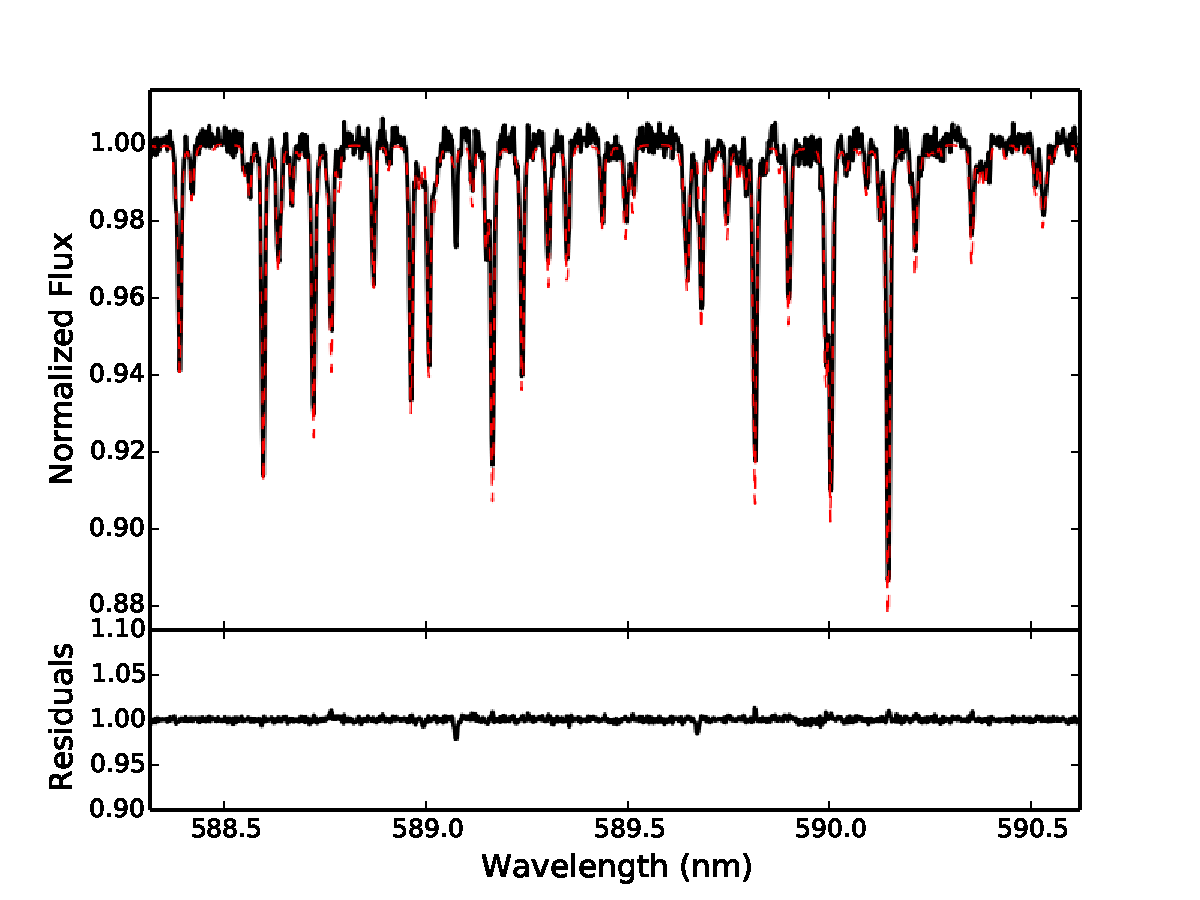
\includegraphics[width=0.4\textwidth, height=0.23\textheight]{Figures/paper3_BstarCorr_590nm.pdf}} 
\subfloat{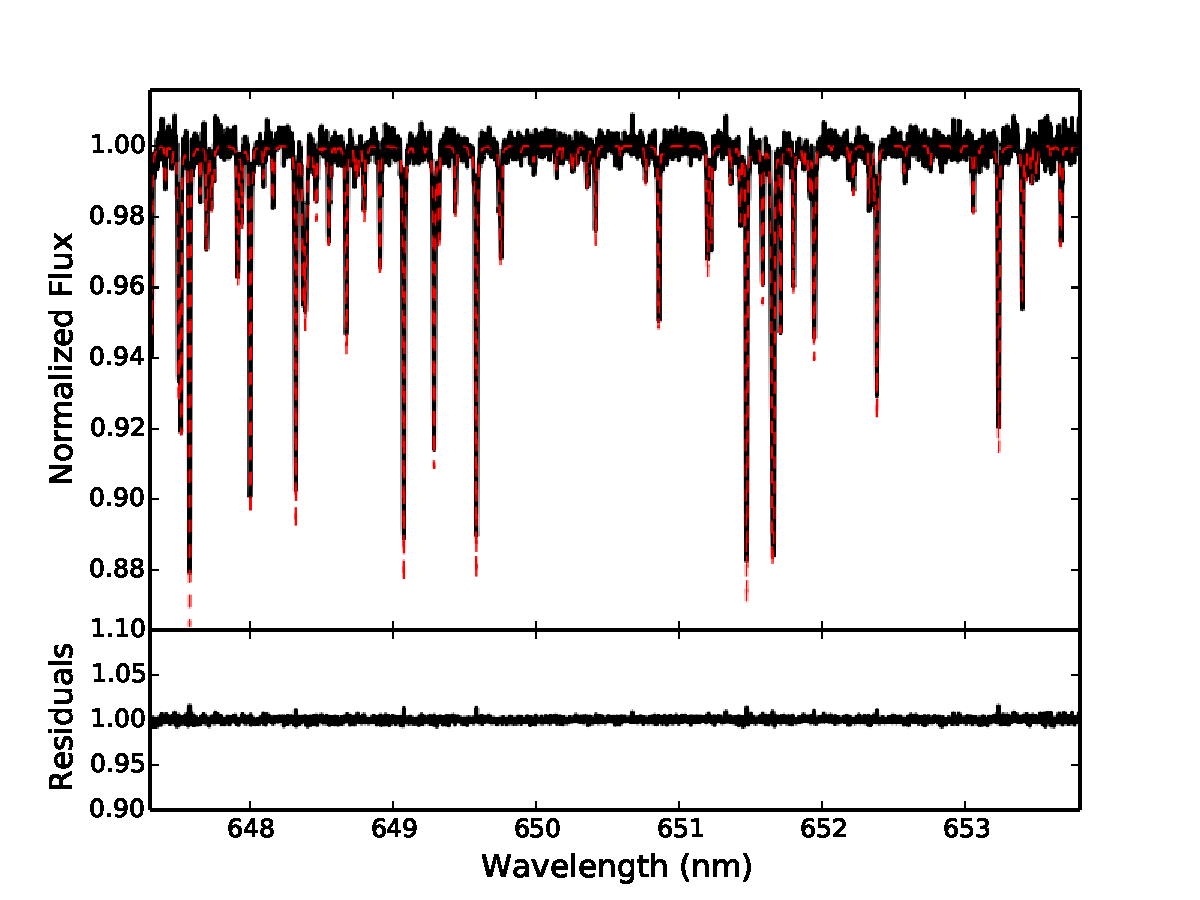
\includegraphics[width=0.4\textwidth,height=0.23\textheight]{Figures/paper3_BstarCorr_650nm.pdf}}
\\
\noindent 
\subfloat{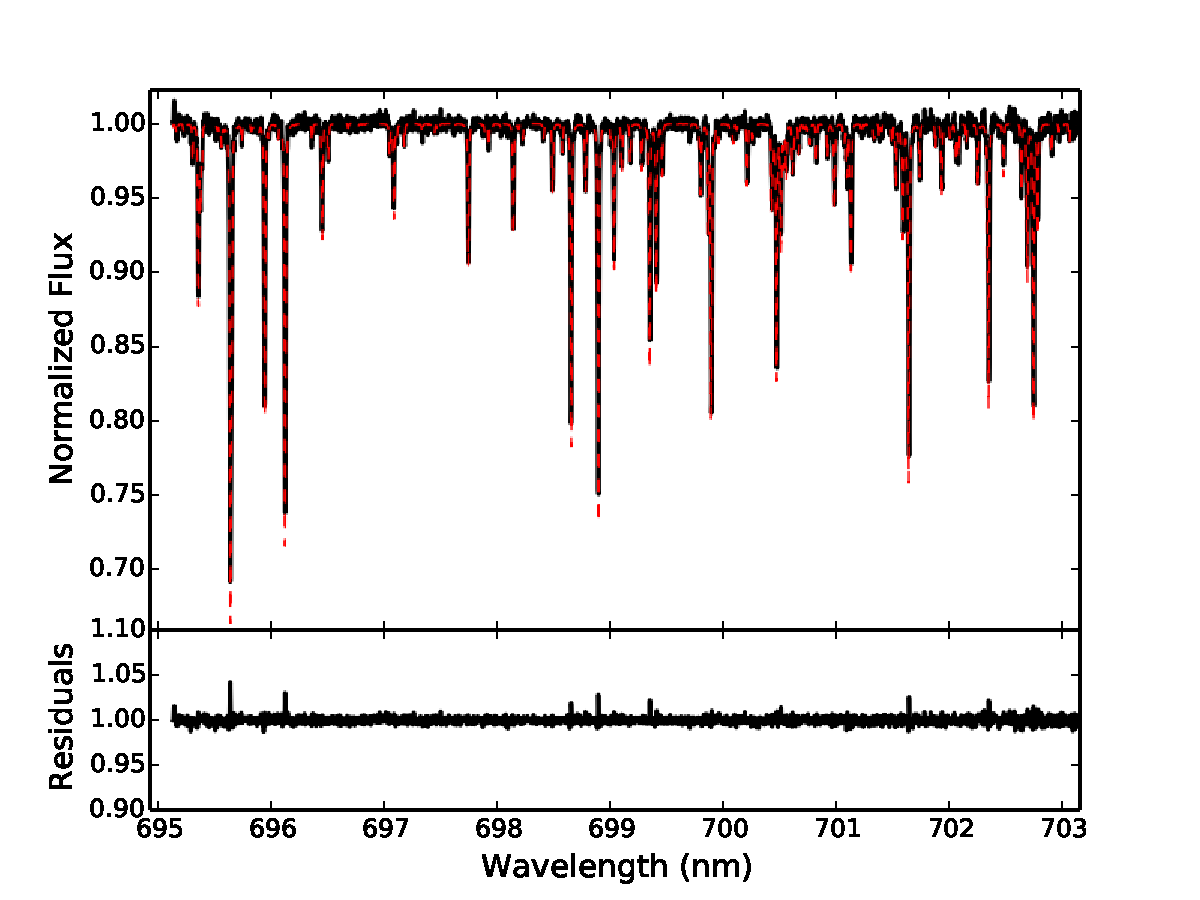
\includegraphics[width=0.4\textwidth, height=0.23\textheight]{Figures/paper3_BstarCorr_700nm.pdf}} 
\subfloat{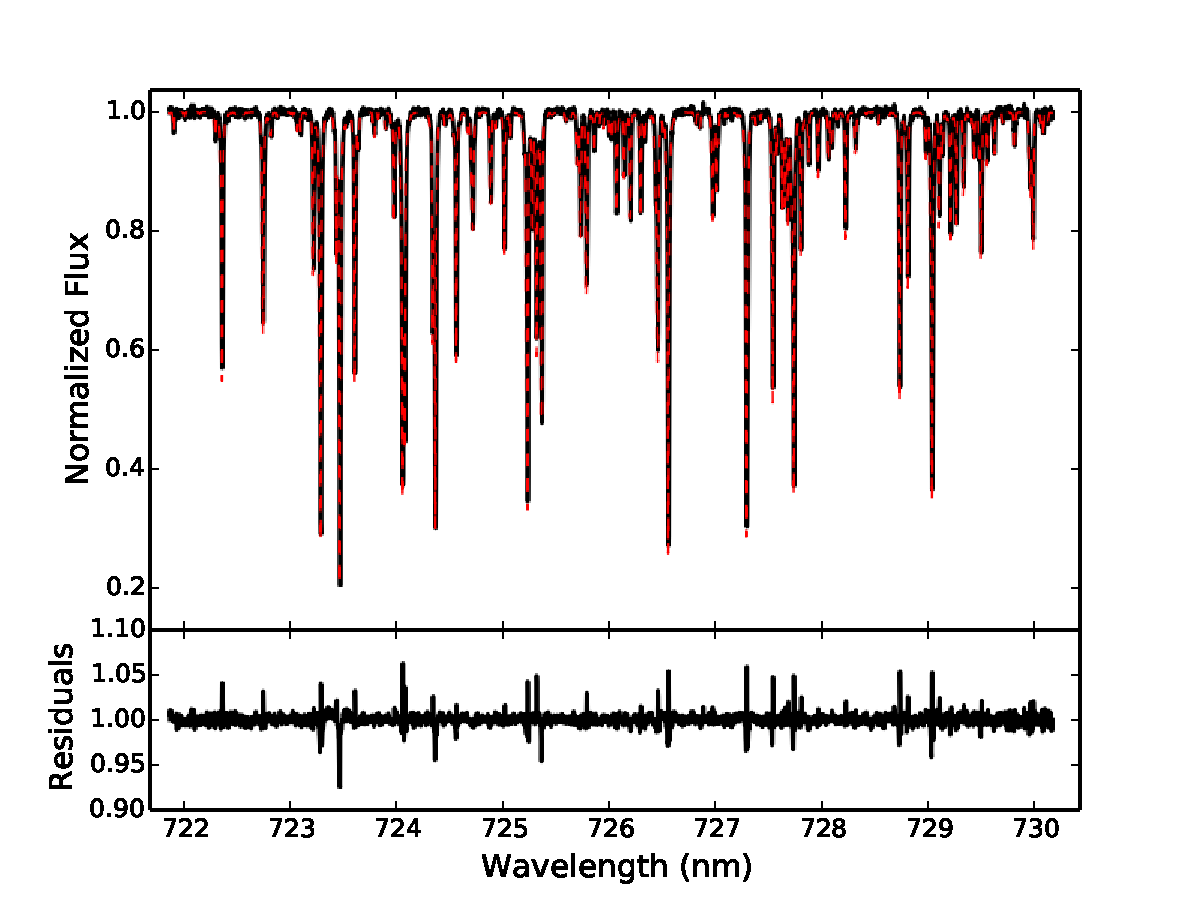
\includegraphics[width=0.4\textwidth,height=0.23\textheight]{Figures/paper3_BstarCorr_730nm.pdf}}
\caption{Correction of the water bands in optical spectra. All spectra are of the A0V star HIP 20264, and are smoothed with a Savitzky-Golay filter after telluric correction to remove any broad features in the stellar spectrum. The top panel of each figure shows the observed spectrum (black solid line) and the best-fit telluric model (red dashed line), and the bottom panel shows the residuals after division by the telluric model. The telluric water lines are corrected to very near the noise level of the spectrum in the top row, revealing weak interstellar Na D lines (top left). The telluric correction leaves residuals on the order of $5\%$ of the continuum for strong telluric lines (bottom right), possibly due to an incorrect atmosphere profile for water vapor.}

\label{paper3_fig:bstarcorr_water}
\end{center}
\end{figure}


%--------------------------------------------------------------------------------------

\begin{figure}
\begin{center}
\subfloat{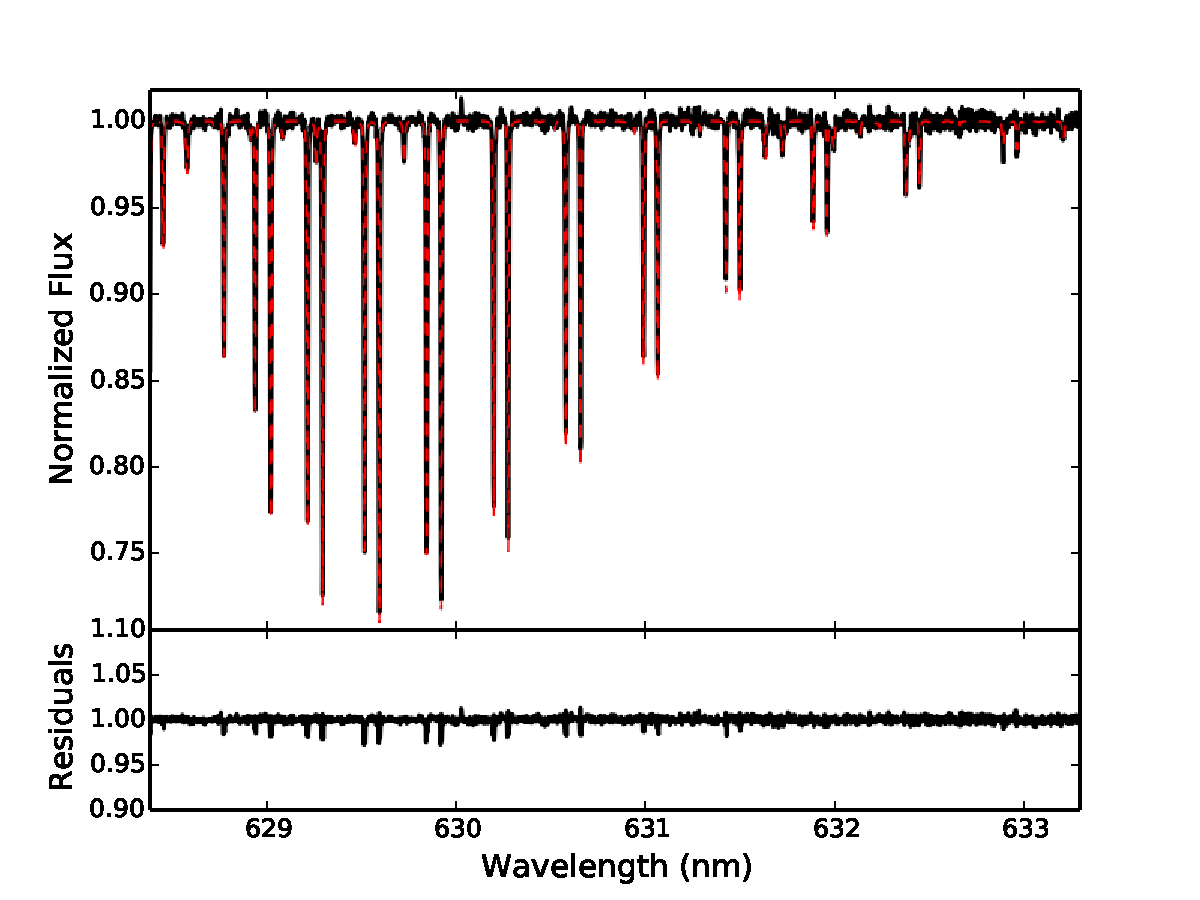
\includegraphics[height=0.33\textheight]{Figures/paper3_BstarCorr_630nm.pdf}}
\\ 
\subfloat{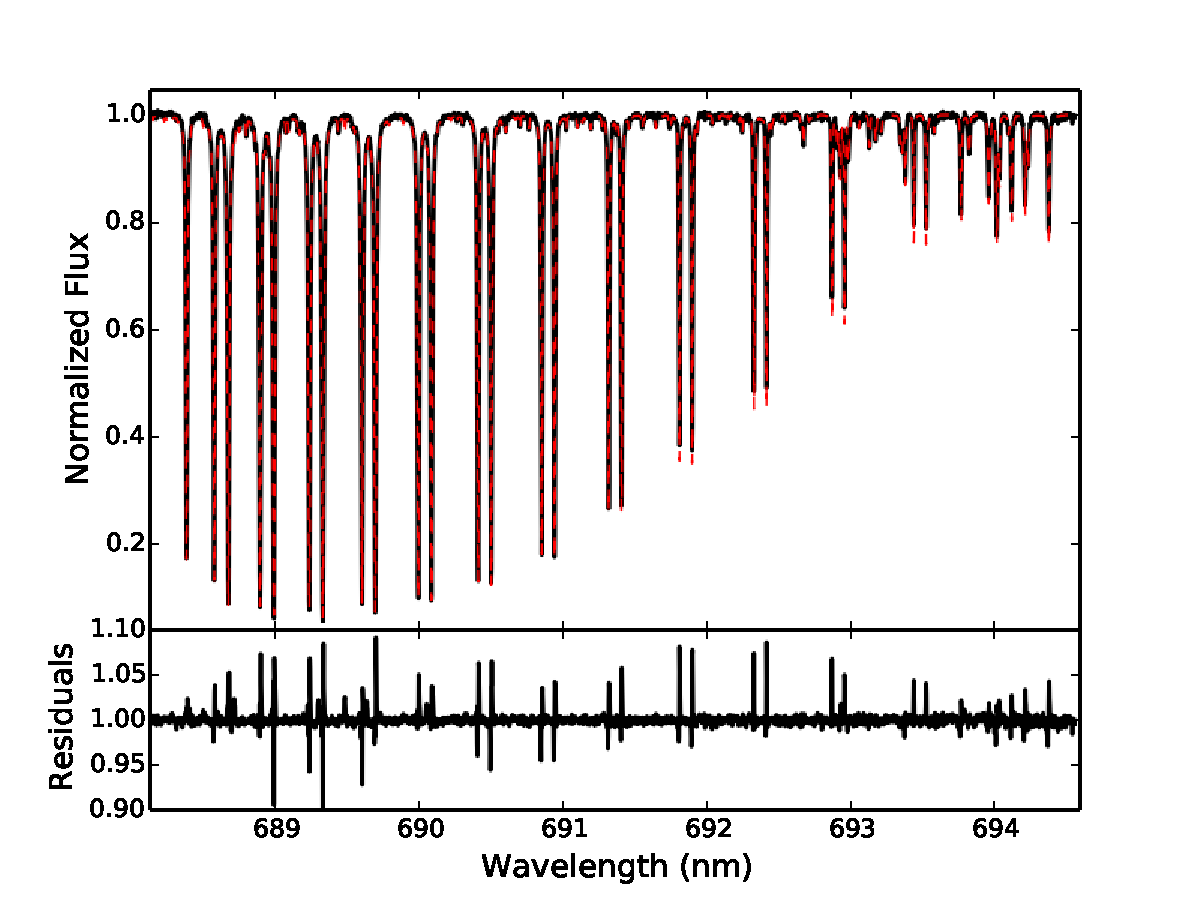
\includegraphics[height=0.33\textheight]{Figures/paper3_BstarCorr_690nm.pdf}}
\caption{Correction of the $\mathrm{O_2}$ bands in optical spectra. All spectra are of the A0V star HIP 20264, and are smoothed with a Savitzky-Golay filter after telluric correction to remove any broad features in the stellar spectrum. The top panel of each figure shows the observed spectrum (black solid line) and the best-fit telluric model (red dashed line), and the bottom panel shows the residuals after division by the telluric model. }

\label{paper3_fig:bstarcorr_oxygen}
\end{center}
\end{figure}

%--------------------------------------------------------------------------------------

\begin{figure}
\begin{center}
\subfloat{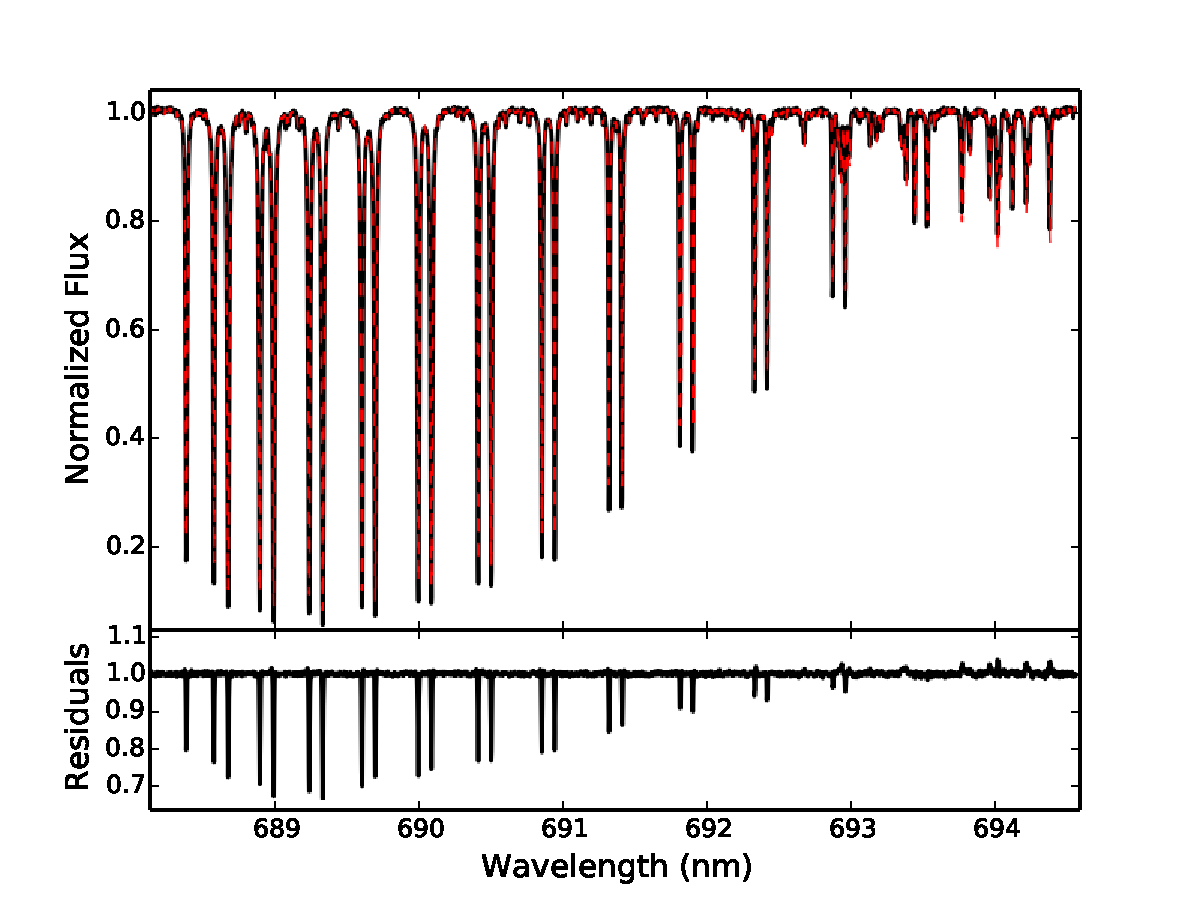
\includegraphics[width=0.4\textwidth,height=0.23\textheight]{Figures/paper3_Empirical_690nm.pdf}}
\subfloat{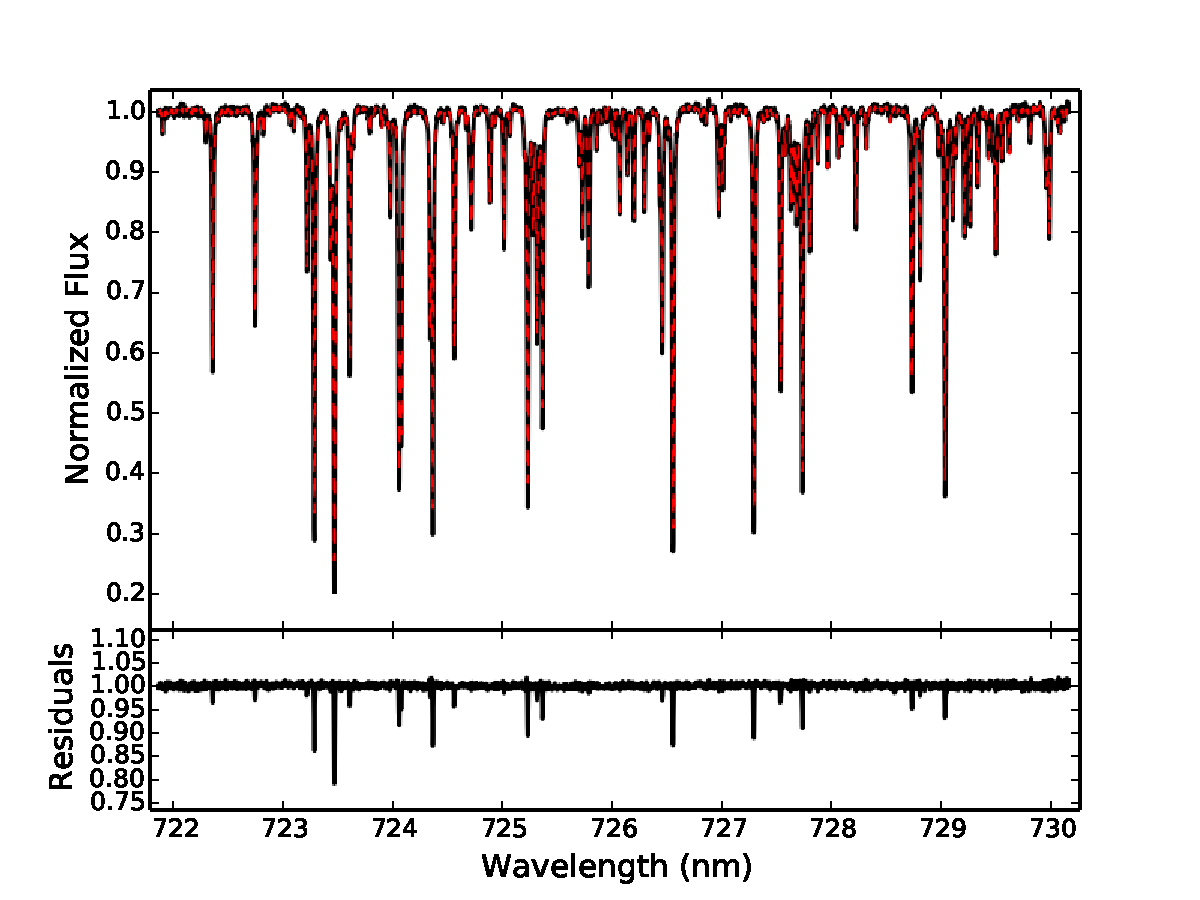
\includegraphics[width=0.4\textwidth,height=0.23\textheight]{Figures/paper3_Empirical_730nm.pdf}}
\\ 
\subfloat{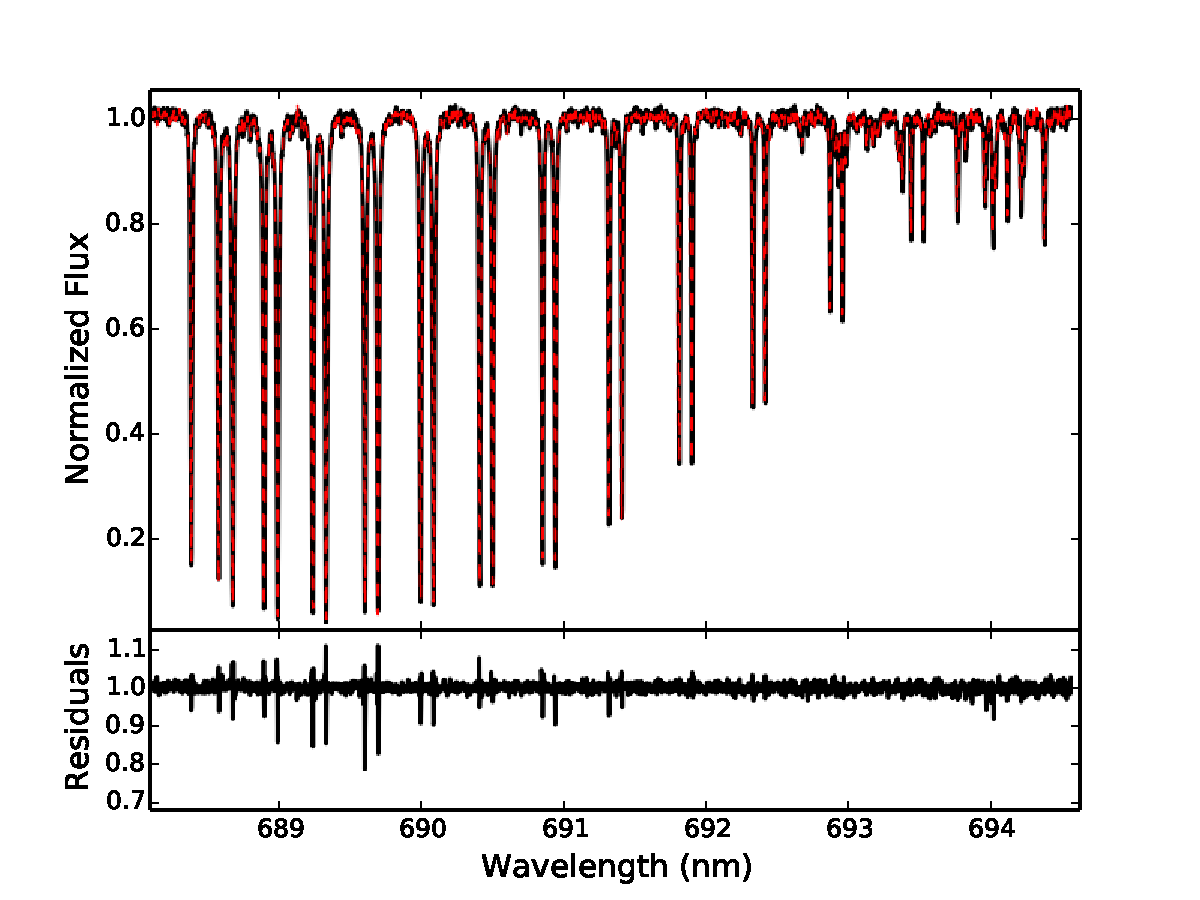
\includegraphics[width=0.4\textwidth,height=0.23\textheight]{Figures/paper3_Empirical_LowSN_690nm.pdf}}
\subfloat{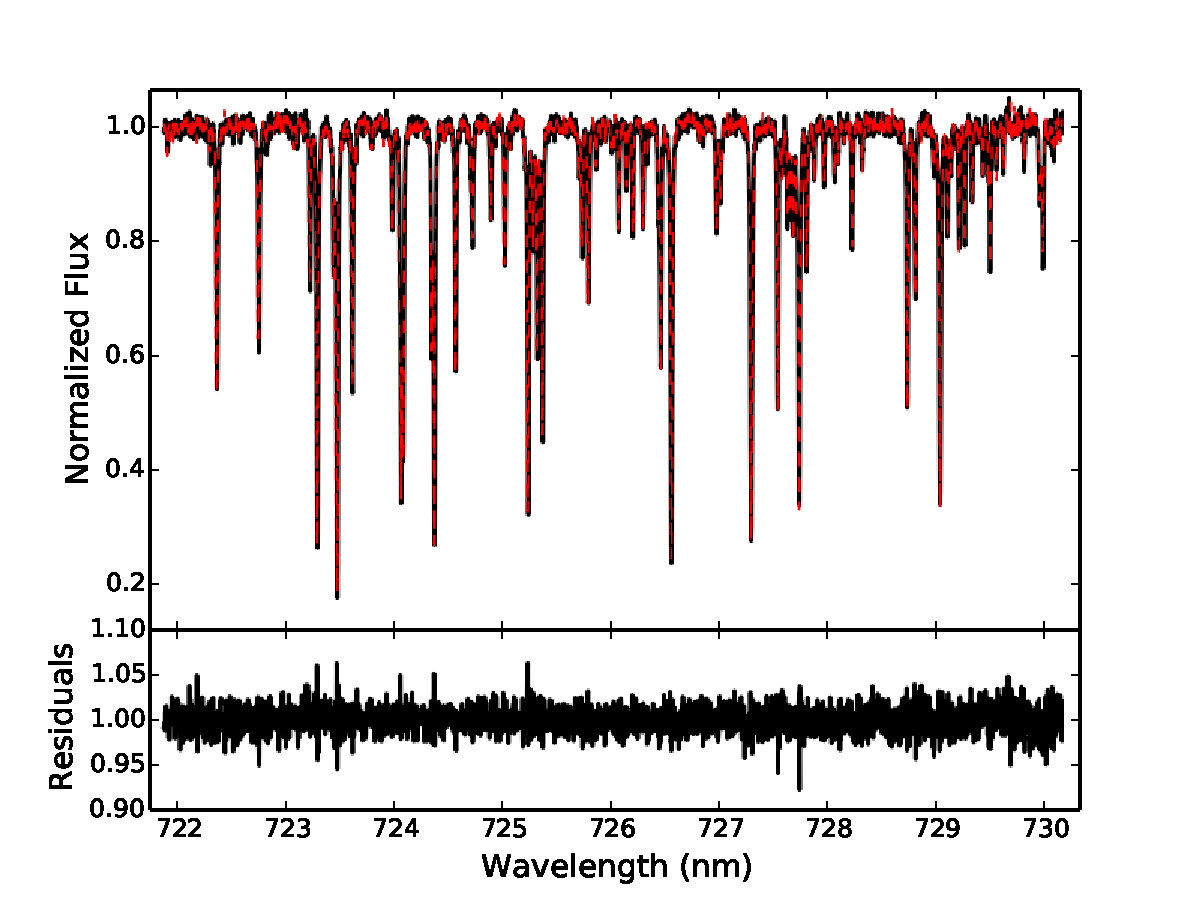
\includegraphics[width=0.4\textwidth,height=0.23\textheight]{Figures/paper3_Empirical_LowSN_730nm.pdf}}
\caption{Empirical telluric corrections. \emph{Top Row}: Correction at high S/N ratio, where all 7 frames of both the target star (HIP 20264, A0V) and the telluric standard star (HIP 25608, A1V) were co-added before the telluric correction. In this case, both the humidity and the airmass are changing throughout both exposures and the empirical telluric correction is very poor. \emph{Bottom Row}: Correction between the last frame taken of the target star and the first frame of the standard star, a more common mode of empirical correction. In this case, the empirical telluric correction is comparable to the model fitting method presented in this paper. The left column should be compared to the bottom panel in Figure \ref{paper3_fig:bstarcorr_oxygen}, and the right column should be compared to the bottom right subfigure in Figure \ref{paper3_fig:bstarcorr_water}. The poor correction in the oxygen band (lower left panel) is the result of the slight airmass difference between the science and standard stars. The correction in equation \ref{paper3_eqn:correction} is only valid for weak or moderate lines, and does not work as well for the nearly saturated lines shown here. The empirical correction under-corrects the line core while over-correcting the wings.}

\label{paper3_fig:bstarcorr_empirical}
\end{center}
\end{figure}


%--------------------------------------------------------------------------------------


\begin{figure}[ht]
  \centering
  \subfloat{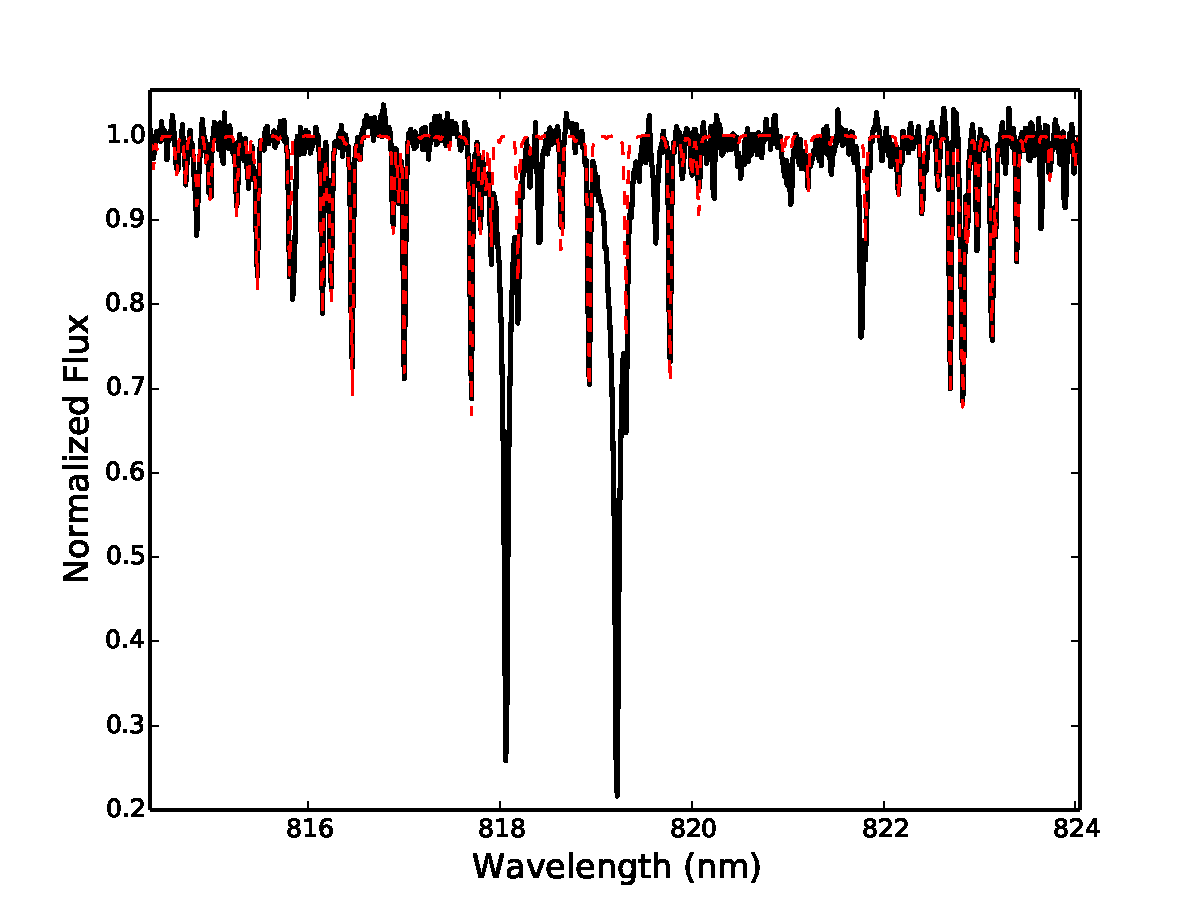
\includegraphics[height=0.33\textheight]{Figures/paper3_GJ908_Telluric.pdf}}
  \\
  \subfloat{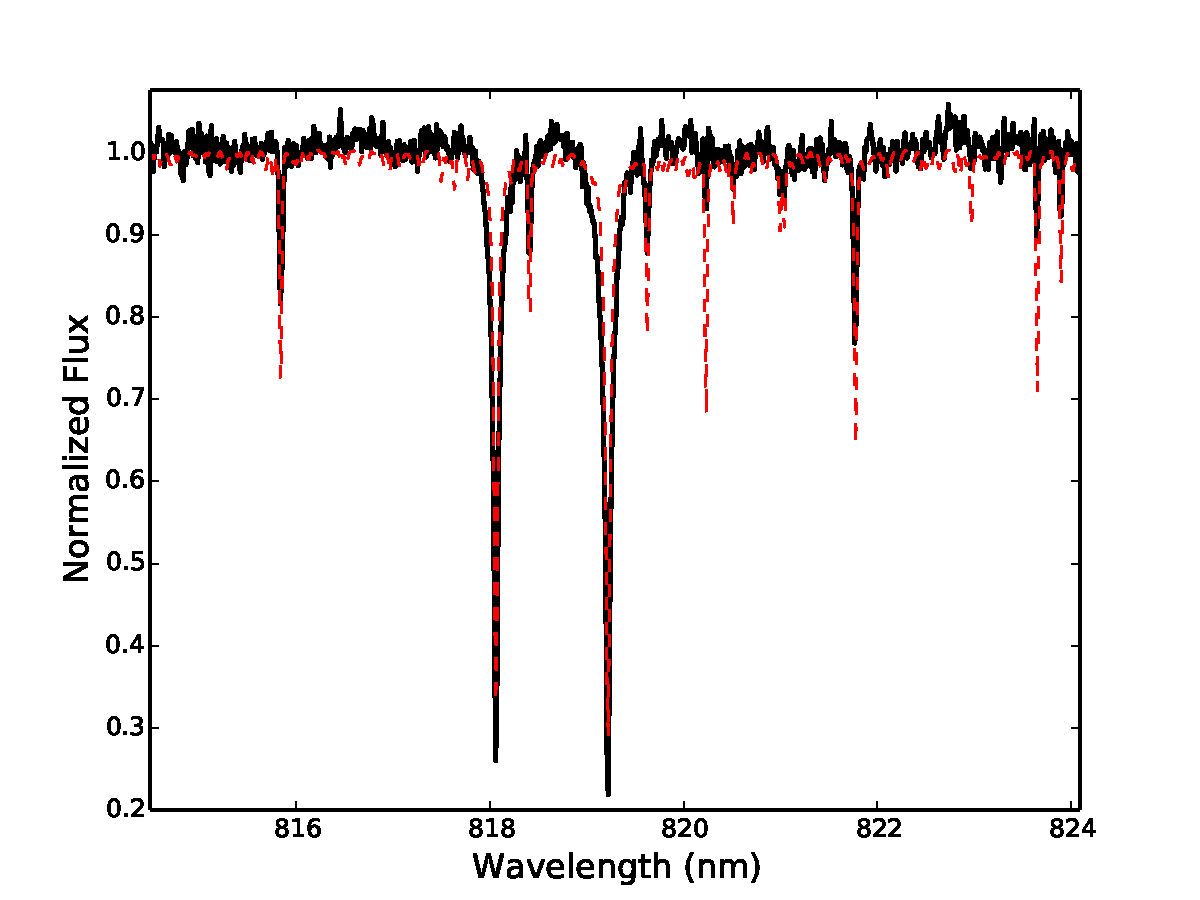
\includegraphics[height=0.33\textheight]{Figures/paper3_GJ908_Stellar.pdf}}
  \caption{\emph{Top}: The observed spectrum of GJ 908 (black solid line) with the best-fit telluric spectrum (red dashed line) overplotted. There are telluric lines within the sodium doublet line profiles which affect any line shape measurements if they are not corrected. \emph{Bottom}: The telluric-corrected spectrum of GJ 908 (black solid line) with a PHOENIX model spectrum (red dashed line) overplotted to guide the eye. The model spectrum has the following parameters: $\mathrm{T_{eff}} = 3700 K$, $\log g = 4.0$, and $\mathrm{[Fe/H]} = -0.5$, and has been convolved with a gaussian to match the detector resolution. All of the remaining absorption lines in the spectrum come from the star.}
  
  \label{paper3_fig:mtellcorr}
\end{figure}

%--------------------------------------------------------------------------------------

\begin{figure}[ht]
  \centering
  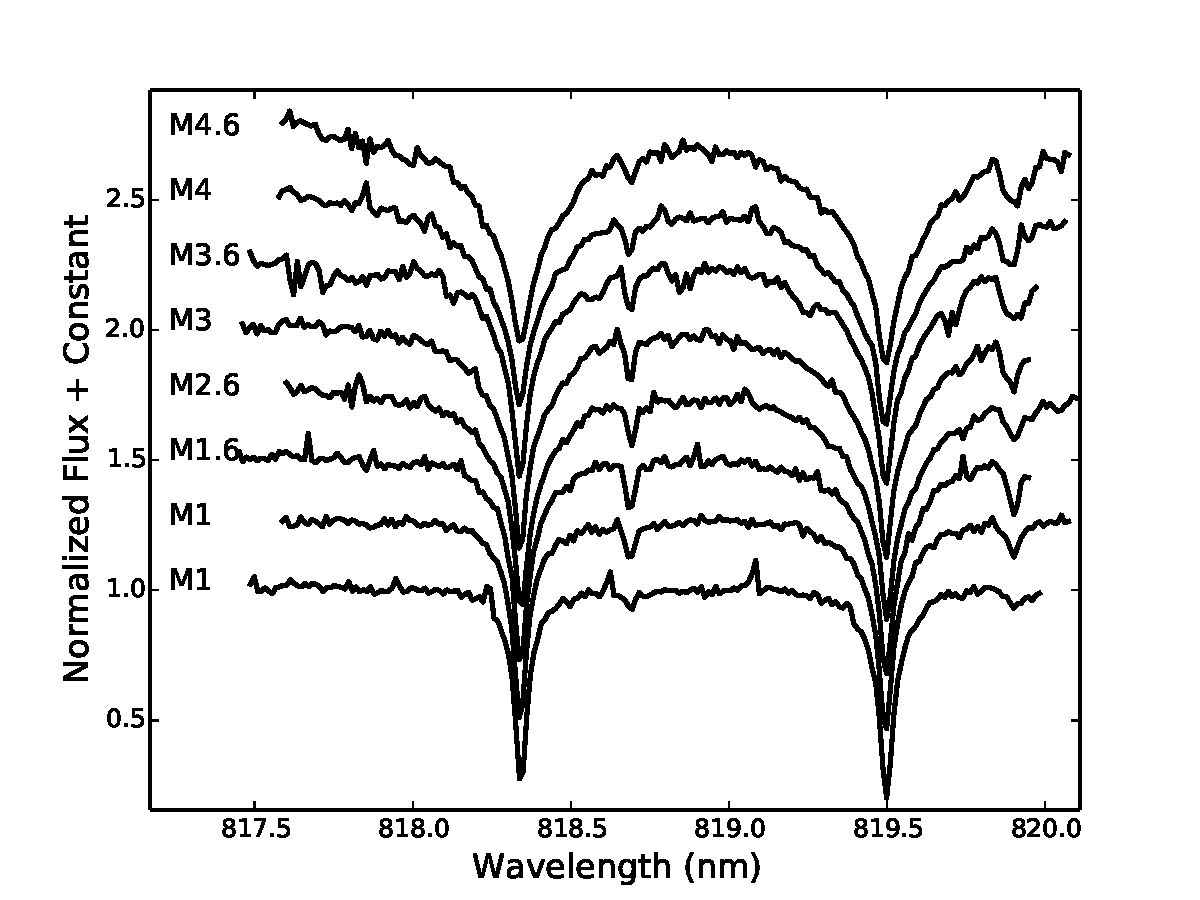
\includegraphics[width=\columnwidth]{Figures/paper3_SodiumLineProfile_BW.pdf}
  \caption{The evolution of the sodium doublet line profile with spectral type for a series of main-sequence M-type stars. The later spectral types show significantly broader line wings.}
  \label{paper3_fig:lineprofile}
\end{figure}




%%%%%%%%%%%%%%%%%%%%%%%%%%%%%%%%%%%%%%%%%%%%%%%%%%
% Chapter 3 (Ps1 Dra A search)
%%%%%%%%%%%%%%%%%%%%%%%%%%%%%%%%%%%%%%%%%%%%%%%%%%




\chapter{Mining Planet Search Data for Binary Stars: The $\psi^1$ Draconis system}
\label{chap:psi1dra}
We now turn to our first case study in using the direct spectral detection method to find a faint companion to the bright star $\psi^1$ Draconis. in this chapter, we use archival data originally obtained in order to search for planetary companions. This chapter was previously published \citep{Gullikson2015}. The co-authors noticed a trend in the data, and suggested I look into it with the direct spectral detection methodology. They obtained the majority of the data used in the work.

\section{Introduction}
\label{paper4_sec:intro}
Several groups \citep[e.g.][]{Wittenmyer2006, Fischer2009, Pepe2011} have used the radial velocity method to search for planets around nearby stars for well over a decade, and have collectively uncovered several hundred planets to date. Close binary stars are usually cut from the star sample because they complicate the detection method \citep[e.g.][]{Bergmann2015}, and because they have long been suspected to inhibit planet formation by quickly destroying \citep{Kraus2012} or depleting \citep{Harris2012} the planet-forming disk.

Previously unknown stellar binary companions are nonetheless still uncovered in planet--search data through large--amplitude linear trends or even full long-period orbits, but may be ignored since the goal is to find planet--mass companions. Since binary stars are usually excluded in the star sample, companions that are found tend to have extreme flux- and mass-ratios. Binary stars with extreme mass-ratios on orbits with $\sim 10$ year timescales are precisely the ones that are most difficult to detect and characterize with imaging techniques, and so they should not be ignored.

Several groups have recently worked towards using high-resolution spectroscopy to search for very faint companions to nearby stars, both in the context of detecting emission \citep{Snellen2010, Gullikson2013} or reflection \citep{Martins2013} from ``Hot Jupiter'' planets, and in the context of detecting stellar binary systems with high contrast ratios \citep[e.g.][]{Gullikson2013_2, Kolbl2015}. Those groups all use a cross-correlation analysis to search directly for the spectral lines of the faint companion and mainly differ in their treatment of the primary star and telluric lines. We describe one method of removing the primary star spectrum in Chapter \ref{chap:dsd}; in this chapter, we describe a second method that uses orbital information to estimate an empirical primary star spectrum.

In this chapter we use data from the McDonald Observatory Planet Search team to examine the $\psi^1$ Draconis system, which consists of an F5IV--V star ($\psi^1$ Dra A) orbited by a G0V star ($\psi^1$ Dra B) with angular separation $30''$ \citep{WDS} (680 AU). \cite{Tokovinin2002} searched for signs of a spectroscopic companion to $\psi^1$ Dra A from 1991--1995, but found no radial velocity variation. More recently \cite{Toyota2009} noted a linear trend in their radial velocity measurements, and predicted a companion with $M > 50 M_J$. Our data have a much longer time baseline than either of the previous studies, and show a significant fraction of the orbit which has recently reached quadrature. Furthermore, \citet{Endl2015} use adaptive-optics imaging to detect a $\sim 4500\ K$ companion 155 mas from $\psi^1$ Dra A, which they hypothesize is the source of the orbital motion seen in the primary-star radial-velocity measurements. 

Here, we use all of our spectra of $\psi^1$ Dra A to search directly for the spectral lines of the companion and measure the system mass ratio. We describe the observations and data reduction in Section \ref{paper4_sec:obs}, and the method we use to search for the companion in Section \ref{paper4_sec:method}. Finally, we estimate the mass-ratio of the system and give the parameters for the companion in Section \ref{paper4_sec:orbit}.


\section{Observations and Data Reduction}
\label{paper4_sec:obs}
All data were taken at the 2.7 m Harlan J. Smith Telescope at McDonald observatory using the 2dcoud\'e \'echelle spectrograph \citep{TS23} at a resolving power $R\equiv \frac{\lambda}{\Delta \lambda} = 60000$. The starlight was filtered through a temperature-stabilized $I_2$ cell to imprint many sharp absorption lines on each spectrum to use for both a precise velocity metric \citep{Butler1996} and to model the instrument profile \citep{Endl2000}. The raw CCD data were reduced with standard IRAF\footnote{IRAF is distributed by the National Optical Astronomy Observatories, which are operated by the Association of Universities for Research in Astronomy, Inc., under cooperative agreement with the National Science Foundation.} tasks, and include steps for overscan trimming, bad--pixel processing, bias--frame subtraction, scattered--light removal, flat--field division, order extraction, and wavelength solution fitting using a Th--Ar calibration lamp spectrum. Particularly strong cosmic--ray hits were removed manually by interpolating across nearby pixels.

We used the \emph{Austral} code \citep{Endl2000} to measure the differential radial velocity of $\psi^1$ Dra A at each observation by comparing each spectrum to a high signal-to-noise ratio template spectrum of the same star. We provide the raw velocity measurements in Table \ref{paper4_tab:rv_data}, as well as the velocities shifted into the system velocity rest frame. The velocity shift necessary to convert from the differential radial velocities to that frame is found in Section \ref{paper4_sec:orbit}. Table \ref{paper4_tab:rv_data} also gives the measurements of the companion radial velocity (described in the next section).


\begin{small}
\begin{longtable}{lrrrrrr}
    
    \caption{The velocities in the `raw' columns are our actual measurements. Those in the `shifted' columns are shifted into the system velocity rest frame using the results of the orbital fit described in Section \ref{paper4_sec:orbit}.} \\
  \label{paper4_tab:rv_data}

    \\ \hline
    Julian Date & \multicolumn{3}{c}{Primary RV (km/s)} & \multicolumn{3}{c}{Secondary RV (km/s)} \\
& raw & shifted & $\sigma$  & raw & shifted  & $\sigma$ \\ \hline
    \endfirsthead

    \\ \hline
    Julian Date & \multicolumn{3}{c}{Primary RV (km/s)} & \multicolumn{3}{c}{Secondary RV (km/s)} \\
& raw & shifted & $\sigma$  & raw & shifted  & $\sigma$ \\ \hline
    \endhead

    \hline
    \endfoot

    \hline
    \endlastfoot


 2451809.66 &   1.927 &  -2.174 &   0.013 &  \nodata &  \nodata &  \nodata \\
 2451809.67 &   1.929 &  -2.172 &   0.014 &  \nodata &  \nodata &  \nodata \\
 2452142.68 &   1.841 &  -2.259 &   0.012 &  \nodata &  \nodata &  \nodata \\
 2453319.64 &   2.433 &  -1.668 &   0.011 &  \nodata &  \nodata &  \nodata \\
 2453585.85 &   2.559 &  -1.542 &   0.010 &  \nodata &  \nodata &  \nodata \\
 2453585.88 &   2.550 &  -1.551 &   0.011 &  \nodata &  \nodata &  \nodata \\
 2453634.64 &   2.654 &  -1.446 &   0.011 &  \nodata &  \nodata &  \nodata \\
 2453635.62 &   2.554 &  -1.547 &   0.009 &  \nodata &  \nodata &  \nodata \\
 2453655.64 &   2.711 &  -1.390 &   0.009 &  \nodata &  \nodata &  \nodata \\
 2453655.64 &   2.780 &  -1.321 &   0.027 &  \nodata &  \nodata &  \nodata \\
 2453689.54 &   2.665 &  -1.436 &   0.008 &  \nodata &  \nodata &  \nodata \\
 2453907.85 &   2.960 &  -1.141 &   0.011 &  \nodata &  \nodata &  \nodata \\
 2453928.80 &   2.858 &  -1.243 &   0.012 &  \nodata &  \nodata &  \nodata \\
 2454019.60 &   2.930 &  -1.171 &   0.012 &  \nodata &  \nodata &  \nodata \\
 2454279.75 &   3.068 &  -1.033 &   0.011 &  \nodata &  \nodata &  \nodata \\
 2454279.76 &   3.056 &  -1.044 &   0.010 &  \nodata &  \nodata &  \nodata \\
 2454309.79 &   3.021 &  -1.080 &   0.013 &  \nodata &  \nodata &  \nodata \\
 2454345.63 &   3.270 &  -0.830 &   0.010 &  \nodata &  \nodata &  \nodata \\
 2454401.56 &   3.155 &  -0.945 &   0.009 &  \nodata &  \nodata &  \nodata \\
 2454662.93 &   3.349 &  -0.752 &   0.015 &    -4.34 &     0.36 &     0.37 \\
 2454665.77 &   3.486 &  -0.615 &   0.014 &    -3.95 &     0.75 &     0.35 \\
 2454665.77 &   3.492 &  -0.609 &   0.015 &    -4.06 &     0.64 &     0.36 \\
 2454730.71 &   3.457 &  -0.644 &   0.014 &    -4.09 &     0.68 &     0.36 \\
 2455100.57 &   3.875 &  -0.226 &   0.016 &    -5.14 &     0.04 &     0.44 \\
 2455100.58 &   3.891 &  -0.210 &   0.014 &    -5.02 &     0.16 &     0.44 \\
 2455398.75 &   4.209 &   0.108 &   0.015 &    -6.49 &    -0.89 &     0.51 \\
 2455790.72 &   4.977 &   0.876 &   0.021 &    -8.65 &    -2.34 &     0.67 \\
 2455869.58 &   5.211 &   1.111 &   0.017 &    -8.14 &    -1.66 &     0.60 \\
 2455910.57 &   5.321 &   1.221 &   0.018 &    -8.40 &    -1.82 &     0.63 \\
 2455992.02 &   5.538 &   1.437 &   0.012 &    -9.01 &    -2.22 &     0.65 \\
 2456016.93 &   5.659 &   1.558 &   0.014 &    -9.23 &    -2.37 &     0.62 \\
 2456106.78 &   5.784 &   1.683 &   0.015 &   -10.36 &    -3.24 &     0.67 \\
 2456138.84 &   5.944 &   1.844 &   0.020 &   -10.73 &    -3.51 &     0.73 \\
 2456145.65 &   5.947 &   1.846 &   0.025 &   -11.38 &    -4.14 &     0.80 \\
 2456145.66 &   5.929 &   1.828 &   0.018 &   -11.43 &    -4.19 &     0.79 \\
 2456145.66 &   5.965 &   1.864 &   0.018 &   -11.15 &    -3.91 &     0.79 \\
 2456173.73 &   5.955 &   1.854 &   0.018 &   -10.82 &    -3.48 &     0.75 \\
 2456401.97 &   6.964 &   2.864 &   0.014 &   -14.11 &    -5.87 &     0.69 \\
 2456401.97 &   6.941 &   2.841 &   0.012 &   -14.39 &    -6.15 &     0.68 \\
 2456433.74 &   7.238 &   3.138 &   0.013 &   -14.54 &    -6.14 &     0.62 \\
 2456433.74 &   7.209 &   3.108 &   0.012 &   -14.61 &    -6.21 &     0.65 \\
 2456435.87 &   7.208 &   3.108 &   0.015 &   -14.73 &    -6.33 &     0.64 \\
 2456435.87 &   7.205 &   3.104 &   0.015 &   -15.08 &    -6.68 &     0.64 \\
 2456461.87 &   7.358 &   3.257 &   0.012 &   -14.96 &    -6.42 &     0.63 \\
 2456461.88 &   7.351 &   3.250 &   0.015 &   -14.65 &    -6.11 &     0.65 \\
 2456461.88 &   7.326 &   3.225 &   0.016 &   -14.60 &    -6.06 &     0.61 \\
 2456465.80 &   7.297 &   3.196 &   0.014 &   -14.74 &    -6.18 &     0.53 \\
 2456497.86 &   7.574 &   3.473 &   0.019 &   -15.86 &    -7.13 &     0.73 \\
 2456519.62 &   7.765 &   3.664 &   0.015 &   -16.78 &    -7.93 &     0.59 \\
 2456525.66 &   7.725 &   3.624 &   0.017 &   -16.27 &    -7.38 &     0.64 \\
 2456560.58 &   7.812 &   3.711 &   0.013 &   -16.32 &    -7.22 &     0.90 \\
 2456564.59 &   7.781 &   3.680 &   0.015 &   -16.18 &    -7.05 &     0.86 \\
 2456613.55 &   8.089 &   3.988 &   0.016 &   -15.96 &    -6.51 &     0.91 \\
 2456614.58 &   8.139 &   4.038 &   0.012 &   -16.52 &    -7.06 &     0.85 \\
 2456755.98 &   9.308 &   5.208 &   0.014 &   -21.44 &   -10.84 &     0.74 \\
 2456759.97 &   9.366 &   5.265 &   0.015 &   -21.91 &   -11.28 &     0.76 \\
 2456784.84 &   9.603 &   5.502 &   0.017 &   -22.56 &   -11.69 &     0.81 \\
 2456816.67 &   9.895 &   5.794 &   0.014 &   -23.36 &   -12.17 &     0.74 \\
 2456816.67 &   9.907 &   5.806 &   0.015 &   -23.68 &   -12.49 &     0.72 \\
 2456860.73 &  10.402 &   6.301 &   0.016 &   -25.64 &   -13.97 &     0.88 \\
 2456860.73 &  10.421 &   6.321 &   0.015 &   -25.77 &   -14.11 &     0.83 \\
 2456885.62 &  10.607 &   6.507 &   0.015 &   -27.23 &   -15.29 &     0.84 \\
 2456938.63 &  11.189 &   7.089 &   0.016 &   -29.30 &   -16.77 &     1.03 \\
 2456938.64 &  11.173 &   7.072 &   0.015 &   -28.99 &   -16.45 &     0.96 \\
 2457092.02 &  12.114 &   8.013 &   0.015 &   -31.57 &   -18.09 &     1.00 \\
 2457109.85 &  12.077 &   7.976 &   0.015 &   -32.79 &   -19.40 &     1.10 \\
 2457118.96 &  11.987 &   7.886 &   0.016 &   -31.14 &   -17.82 &     0.90 \\
 2457150.92 &  11.685 &   7.584 &   0.017 &  \nodata &  \nodata &  \nodata \\
 2457174.96 &  11.267 &   7.167 &   0.017 &   -28.58 &   -16.13 &     0.81 \\
 2457214.83 &  10.240 &   6.139 &   0.017 &   -24.68 &   -13.16 &     0.82 \\
 2457214.84 &  10.253 &   6.152 &   0.016 &   -25.36 &   -13.85 &     0.90 \\
 2457216.73 &  10.220 &   6.119 &   0.016 &   -25.13 &   -13.66 &     0.86 \\
 2457216.73 &  10.228 &   6.128 &   0.015 &   -25.15 &   -13.69 &     0.80 \\
 2457245.60 &   9.302 &   5.201 &   0.016 &   -22.21 &   -11.52 &     0.77 \\
 2457245.61 &   9.299 &   5.199 &   0.016 &   -21.85 &   -11.16 &     0.72 \\
 2457248.61 &   9.338 &   5.237 &   0.017 &   -21.66 &   -11.05 &     0.70

  
\end{longtable}
\end{small}




 
 
 


\section{Companion Search}
\label{paper4_sec:method}

We use a cross-correlation analysis inspired by recent work attempting to detect light from planetary companions around late-type stars \citep{Gullikson2013, Martins2013} to search for the companion ($\psi^1$ Dra C). We start by dividing all spectra by the blaze function of the spectrograph, and further divide them by an empirical $I_2$ cell absorption spectrum in the spectral orders with $500 < \lambda < 640$ nm. The blaze function is derived by fitting a high-order polynomial to the extracted spectrum of an incandescent light source (a flat lamp), and the empirical $I_2$ spectrum is the spectrum of a flat lamp with the $I_2$ cell inserted in the light path. Both the flat lamp and $I_2$ spectra are observed each day of each observing run. We use the Telfit code \citep[][and Chapter \ref{chap:telfit}]{Gullikson2014} to fit and remove the unsaturated telluric absorption lines in the spectrum, and cross-correlate each residual spectrum against a Phoenix model spectrum \citep{Husser2013} with parameters

\begin{itemize}
\item $T_\mathrm{eff} = 4400$ K
\item $\log{g} = 4.5$ (cgs units)
\item {[}Fe/H{]} = 0.0
\end{itemize}

The model temperature was chosen on the basis of high--contrast imaging in \citet{Endl2015}, which finds a companion with approximately that temperature. We shift each CCF so that the dominant peak, which signifies the match of the M-star model template with the F-type primary star, falls at $v=0$. That effectively puts the cross-correlation functions in the rest frame of the primary star, although there is a constant velocity offset caused by small errors in the vacuum to air wavelength conversion and spectrograph wavelength drift throughout the night. We denote this shift as $\Delta v_2$ in later sections of this paper.

We normalize each CCF by subtracting a quadratic function that we fit well away from the peak, and then dividing by the height of the CCF at $v=0$ (the peak). The average of the shifted CCFs is a close estimate for the cross-correlation function of the M-star template with the F5 primary star, since the contribution from the companion is diluted by shifting the CCFs to the primary star rest frame. We remove the contribution from the primary star by subtracting the average from each CCF. The result is a series of residual cross-correlation functions that are estimates for the CCF of the companion spectrum against the 4400 K model spectrum template, with significant noise. We show the residual CCFs in Figure \ref{paper4_fig:resids}; the trace of the companion star is easily visible as the dark curve near the top middle. We are unable to recover the companion signal at early dates when the two stars were close to one another in velocity space.



\begin{figure}[t]
  \centering
  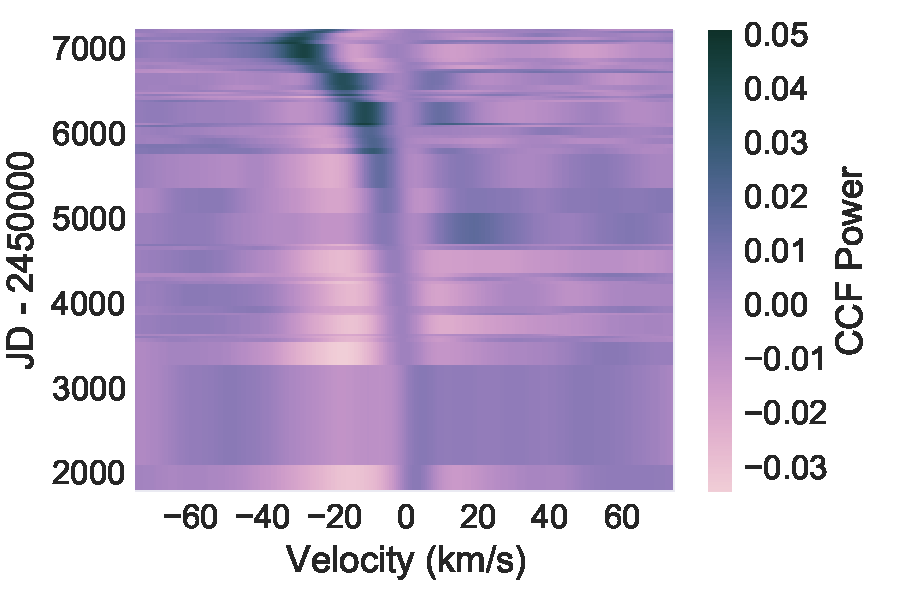
\includegraphics[width=\columnwidth]{Figures/paper4_Resid_CCFs.pdf}
  \caption{Cross-correlation functions of a 4400 K model spectrum template with the data, after subtraction of the average CCF. The dark curve in the top middle is the signal of the companion star.}
  \label{paper4_fig:resids}
\end{figure}



\begin{figure}[t]
  \centering
  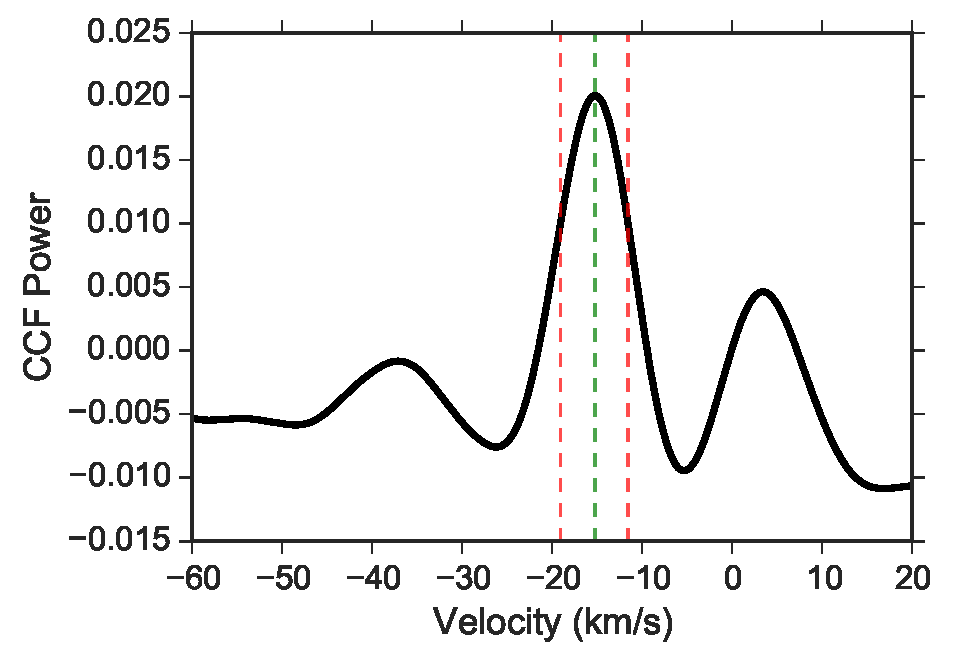
\includegraphics[width=\columnwidth]{Figures/paper4_Typical_CCF.pdf}
  \caption{An example of a typical residual cross-correlation function. The dominant peak denotes the template match of the 4400 K template with the companion to $\psi^1$ Draconis A. The velocities are in the approximate rest frame of the primary star (see text for details), and the centroid and FWHM are given as vertical dotted lines.}
  \label{paper4_fig:ccf_typical}
\end{figure}




We measure the radial velocity of the companion at each epoch by finding the maximum and full-width-half-maximum (FWHM) of the residual CCF. On the basis of Figure \ref{paper4_fig:resids}, we use only the portion of the CCFs with $-50 < v < 10\ \mathrm{km\ s}^{-1}$; we show a typical residual CCF in Figure \ref{paper4_fig:ccf_typical}. Since the CCFs were shifted to subtract the contribution from the primary star, the measured velocities ($v_{m, 2}$) are related to the true barycentric velocities ($v_1$ and $v_2$ for the primary and secondary, respectively) and the constant shift described above ($\Delta v_2$) through

\begin{equation}
v_{m, 2}(t) = v_2(t) - v_1(t) + \Delta v_2
\label{paper4_eqn:vel}
\end{equation}

We give the measured companion velocities in Table \ref{paper4_tab:rv_data} (column 5). We additionally provide the velocities in the system velocity rest--frame ($v_2$) by using Equation \ref{paper4_eqn:vel} and the results of the analysis described below. The uncertainties given in Table \ref{paper4_tab:rv_data} are determined from the CCF peak width and the scaling factor ($f$) derived below. The shifted primary and secondary velocities given in Table \ref{paper4_tab:rv_data} are for the reader's convenience since they are in the same reference frame; we use the raw measurements in the orbital fit.


\section{Orbital Fit}
\label{paper4_sec:orbit}

We now use the radial--velocity measurements to find the best orbital parameters to describe the orbit, as well as some data scaling and shifting factors. The orbit is described by the semi-amplitudes for both the primary and secondary stars ($K_1$ and $K_2$, respectively), the longitude of pericenter ($\omega$), the eccentricity ($e$), the period ($P$), and the periastron--passage epoch ($T_0$). We cannot measure the system radial velocity, which is usually the final orbital element, because the measured primary--star velocities are differential and the secondary--star velocities are measured relative to the primary star.

Since the primary--star radial velocity measurements are differential measurements, we must also fit a constant shift ($\Delta v_1$) to account for the absolute radial velocity of the primary at the time at which our template spectrum was observed. We include an rv--jitter term ($\sigma_J$) to the fit to account for radial--velocity variations not encompassed by the orbital solution, and add the value in quadrature with the formal uncertainties on the primary star--velocity measurements. 

The companion radial velocities are measured relative to the primary star plus a small velocity shift ($\Delta v_2$) caused by slight inaccuracies in the vacuum--to--air wavelength conversion in the model spectrum and spectrograph wavelength drift throughout the night. Finally, the CCF peak full-width at half maximum vastly over-estimates the velocity uncertainty and so we fit a scale factor ($f$) to apply to the companion velocity uncertainties. The uncertainties given in Table \ref{paper4_tab:rv_data} are already scaled by that factor. The full log-likelihood function ($\mathcal{L}$) is then given by:

\begin{align*}
s_1 &= \sum_{t_m} \frac{(v_{1,m} - v_1(t_m) - \Delta v_1)^2 }{\sigma_{v_1}^2 + \sigma_J^2} + \ln{2\pi(\sigma_{v_1}^2 + \sigma_J^2)} \\
s_2 &= \sum_{t_m} \frac{(v_{2,m} - v_2(t_m)(1+\frac{K_1}{K_2}) - \Delta v_2)^2}{f\sigma_{v_2}^2 } + \ln{2\pi(f\sigma_{v_2}^2)} \\ 
\mathcal{L} &= -0.5(s_1 + s_2) \\
\end{align*}

where $v_{1,2}(t) = v(T_0, P, e, K_{1,2}, \omega, t)$ is the velocity at time t given by the orbital elements $T_0, P, e, K$, and $\omega$.

We use the affine invariant sampler provided in the emcee code \citep{emcee} to perform a Markov Chain Monte Carlo (MCMC) fit to all of the parameters described above. We use flat priors in all variables except for the rv--jitter and companion rv uncertainty scale factors ($\sigma_J$ and $f$, respectively), for which we use log-uniform priors to allow for a large range of values.  We give the median value and uncertainty for each parameter in Table \ref{paper4_tab:orbit}., and display samples from the marginal posterior distributions of the orbital parameters in Figure \ref{paper4_fig:posterior} The uncertainties are estimated from the posterior probability distribution samples such that the lower and upper bounds give the 16th and 84th percentile (i.e. they are $1\sigma$ credibility intervals). We plot the best-fit orbit with the data in Figure \ref{paper4_fig:orbit}, with the uncertainties on the companion velocities scaled and the velocities shifted by $\Delta v_1$ and $\Delta v_2$. 

Next, we calculate a series of derived quantities to characterize the companion and report them in Table \ref{paper4_tab:orbit}. The mass ratio of the system is the ratio $K_1/K_2 = 0.47$. We estimate the primary star mass by interpolating Dartmouth isochrones \citep{Dotter2008} with the `isochrones' code \citep[described in][]{Montet2015}, and using spectroscopic parameters derived in \citet{Endl2015}. The secondary mass is $M_2 = qM_1 \sim 0.70\ M_{\odot}$; assuming the same age and metallicity as the primary, the Dartmouth isochrones give an expected temperature of ${\sim}4400 $ K. That temperature is in excellent agreement with the high--contrast--imaging data, which support a companion of ${\sim}4400$ K with large uncertainty. With both the primary and secondary star mass, we calculate the orbital inclination and semimajor axis and report them in Table \ref{paper4_tab:orbit}.

\begin{figure}[t]
  \centering
  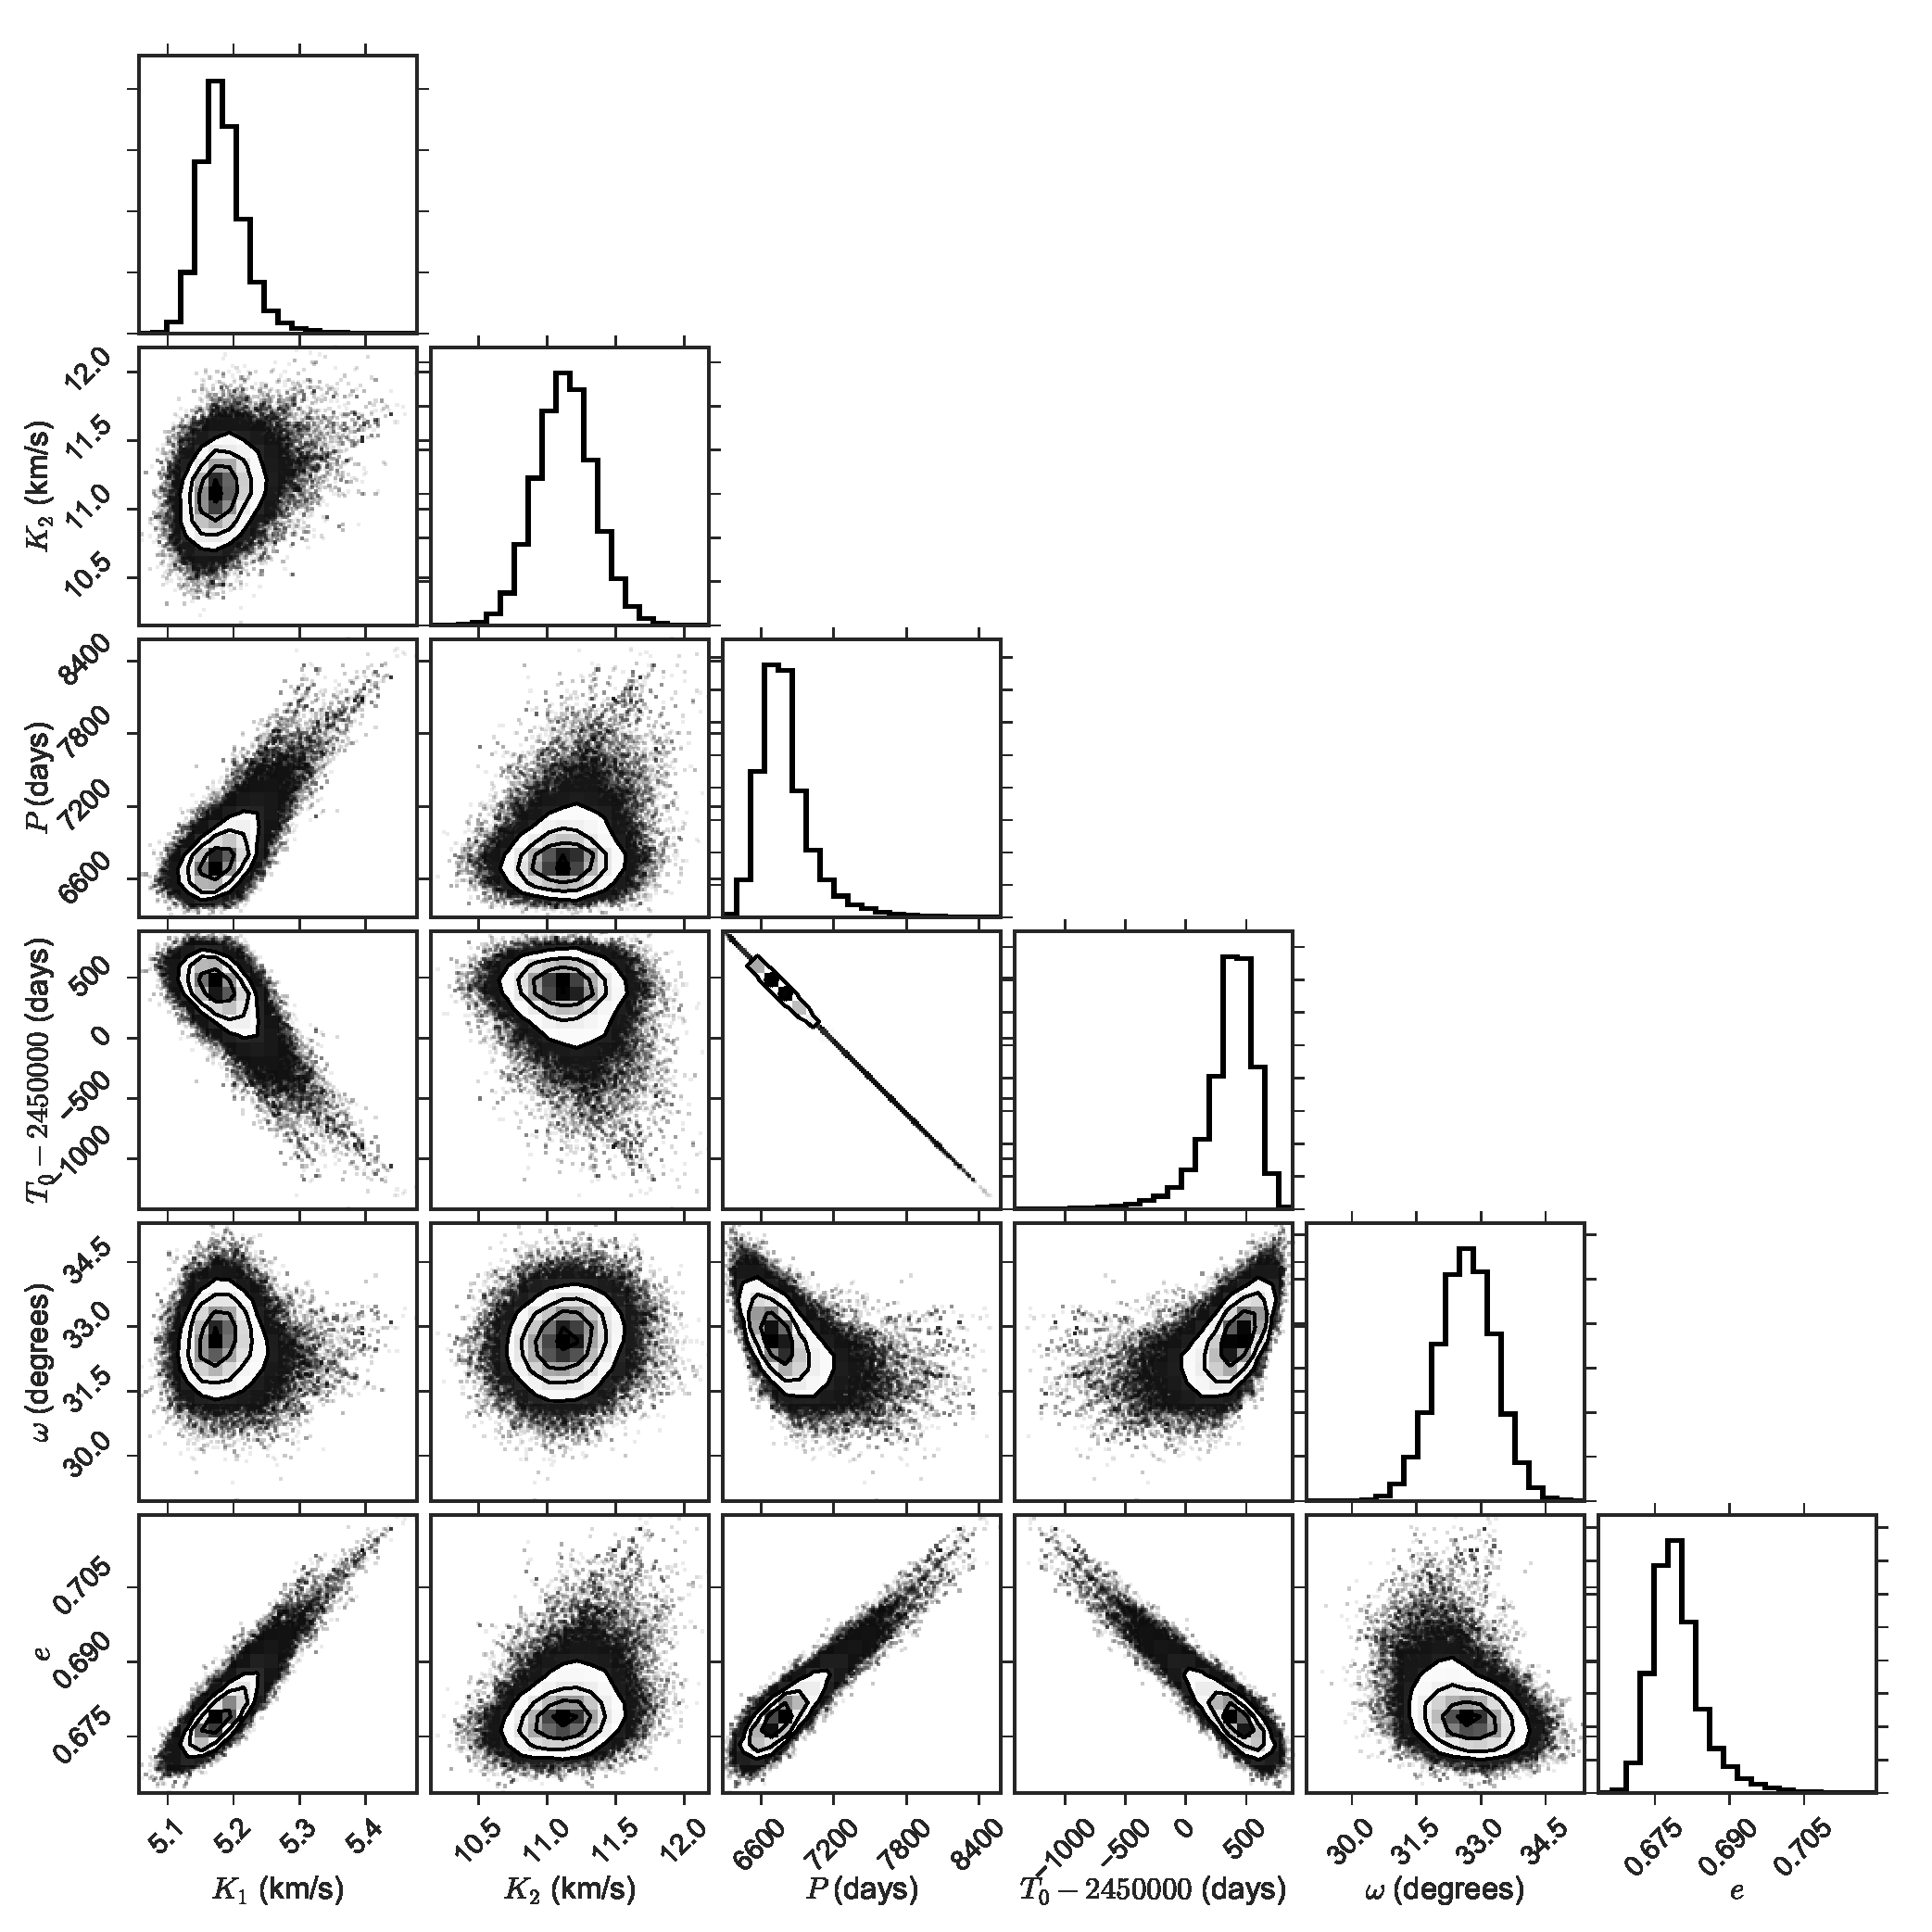
\includegraphics[width=\columnwidth]{Figures/paper4_corner.pdf}
  \caption{Marginalized posterior probability distribution estimates for the orbital parameters we fit. There is a strong degeneracy between the period and epoch of periastron ($T_0$) because we have not yet observed a full orbit.}
  \label{paper4_fig:posterior}
\end{figure}



\begin{table}[t]
  \centering
\caption{The primary mass is derived using the spectroscopic $T_\mathrm{eff}$, $\log{g}$, and [Fe/H] and interpolating Dartmouth isochrones. The companion temperature is likewise derived from the companion mass using Dartmouth isochrones of the same metallicity.}
  \footnotesize
  \begin{tabular}{rl}
    \hline

\multicolumn{2}{c}{\textbf{Parameters from \citet{Endl2015}}} \\
$T_\mathrm{eff,1}$ (K) & $6544 \pm 42$ \\
$\log{g}$ & $3.90 \pm 0.11$ \\
{[}Fe/H{]} & $-0.10 \pm 0.05$ \\ \\

\multicolumn{2}{c}{\textbf{Parameters measured in this work}} \\
$K_1$ ($\mathrm{km\ s}^{-1}$) & $5.18^{+0.04}_{-0.03}$ \\
$K_2$ ($\mathrm{km\ s}^{-1}$) & $11.1 \pm 0.2$ \\
Period (days) & $6774^{+271}_{-167}$ \\
Periastron passage time (JD) & $2450388^{+169}_{-273}$ \\
$\omega$ (degrees) & $32.6 \pm 0.7$ \\
$e$ & $0.679^{+0.006}_{-0.004}$ \\
$\Delta v_1\ (\mathrm{km\ s}^{-1})$ & $4.10^{+0.06}_{-0.09}$ \\
$\Delta v_2\ (\mathrm{km\ s}^{-1})$ & $-5.4^{+0.3}_{-0.2}$ \\
Companion uncertainty scale factor ($f$) & $0.17 \pm 0.02 $\\
rv jitter (m s$^{-1}$) & $72^{+7}_{-5}$ \\
reduced $\chi^2$ & 0.41 \\ \\

\multicolumn{2}{c}{\textbf{Derived Values}} \\
$q$ & $0.466 \pm 0.008$ \\
$M_1$ (M$_{\odot}$) & $1.38^{+0.15}_{-0.08}$ \\
$M_2$ (M$_{\odot}$) & $0.70 \pm 0.07$ \\
$T_\mathrm{eff,2}$ (K) & $4400 \pm 300$ \\
$i$ (degrees) & $31 \pm 1$ \\
$a$ (AU) & $9.1^{+0.4}_{-0.3}$ \\ \hline

  \end{tabular}


\label{paper4_tab:orbit}
\end{table}




\begin{figure}[t]

  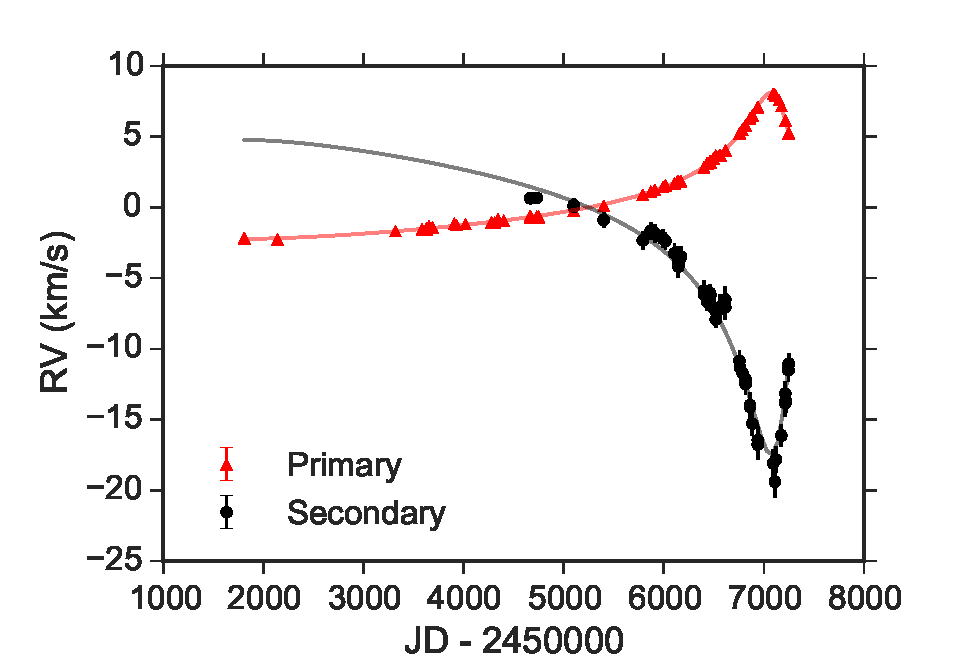
\includegraphics[width=\columnwidth]{Figures/paper4_SB2_Orbit.pdf}
  \caption{Best-fit double-lined orbit for the $\psi^1$ Draconis AC subsystem. There are no measurements of the companion at early dates because they could not be reliably measured in the residual cross-correlation functions.}
  \label{paper4_fig:orbit}
  
\end{figure}



\section{Discussion and Conclusions}

We use nearly 15 years of time-series spectra of the star $\psi^1$ Draconis A to search for the spectral lines of a companion identified by a large--amplitude trend in the primary--star radial velocities and later by direct imaging. We cross-correlate each spectrum against a Phoenix model spectrum of a $4400$ K star and subtract the average CCF. The residual CCFs clearly show the template match with the companion (Figure \ref{paper4_fig:resids}), and we are able to measure the companion radial velocities for most dates. 

We use the radial--velocity measurements for both the primary and secondary stars to find an orbital solution for the now double-lined spectroscopic binary. The summary values of the fitted parameters are given in Table \ref{paper4_tab:orbit}. Finally, we report the mass and expected temperature of the companion as well as the orbital inclination and semi--major axis. The temperature agrees well with high--contrast imaging, validating our method.

The $\psi^1$ Draconis system is therefore a hierarchical multiple system with the component parameters given in Table \ref{paper4_tab:orbit}. $\psi^1$ Dra A and B are separated by ${\sim}680$ AU and have a mass-ratio $q = 0.82$, while A and C (the new companion) have a much closer orbit with with $a = 9.1$ AU and $q = 0.47$. 

This method could be used to search for the spectral lines of stellar companions to other stars observed with high--precision radial--velocity surveys. To that end, and in the goal of open science, we make the source code used for the analysis and generating the plots for this paper available at \url{https://github.com/kgullikson88/Companion-Finder}. The raw radial--velocity measurements for both the primary and secondary star, as well as the MCMC chains, are available at the same url.

This research has made use of the SIMBAD database, operated at CDS, Strasbourg, France, and of Astropy, a community-developed core Python package for Astronomy (Astropy Collaboration, 2013).
It was supported by a start-up grant to Adam Kraus from the University of Texas. The McDonald Observatory planet search is supported by the National Science Foundation under grant AST-1313075. We would like to thank the referee for various suggestions that improved this paper.




%%%%%%%%%%%%%%%%%%%%%%%%%%%%%%%%%%%%%%%%%%%%%%%%%%
% Chapter 4 (IGRINS simulation)
%%%%%%%%%%%%%%%%%%%%%%%%%%%%%%%%%%%%%%%%%%%%%%%%%%




\chapter{Future Direct Spectroscopic Detection of Hot Jupiters with IGRINS}
\label{chap:hotjup}
Several authors have used a variant of the method we described in  Chapter \ref{chap:psi1dra} to search for emission from ``Hot Jupiter`` planets orbiting a sun-like star. In this case the flux ratio is much more extreme, but still possible with enough high signal-to-noise ratio spectra. In this chapter, we generate simulations of the IGRINS instrument to assess whether it can detect Hot Jupiter emission. This chapter was previously published \citep{Gullikson2013}. The co-author, Mike Endl, was my co-supervisor at the time and provided much of the inspiration for the work as well as a great deal of technical assistance. While the instrument was being built at the time of publication, it is now functioning on the 2.7m telescope at McDonald Observatory and a pilot survey based on this work is in progress.


\section{Introduction}
With about 1600 confirmed extrasolar planets \citep[from
exoplanets.org:][]{exoplanet}, the time for characterization of these
planets is here. A first step towards characterization is a determination of
the planet mass. Most of the exoplanets so far discovered around nearby stars were
found using the radial velocity technique, which measures the periodic
Doppler shift of the parent star. Unfortunately, the inclination of the orbit cannot be determined
without another complementary method. This means that planet masses from
radial-velocity surveys are only \emph{minimum} masses. In principle, precise astrometry could provide the complementary measurement that is needed to determine the true planet mass. However, the astrometric motion is very difficult to detect with current technology. The amplitude of the motion of a sun-like star with a Jupiter-mass planet orbiting at 0.1 AU and a distance from Earth of 10 pc is roughly $20 \mu$as, an order of magnitude below the precision of the Hubble Space Telescope Fine Guidance Sensors \citep{Benedict2006} and will be very near the precision of GAIA \citep{Sozzetti2001}.

We can measure the true mass and inclination of a planet only if the
radial velocity of the planet was known as well as that of its parent
star. There are two ways that the
radial velocity of an orbiting planet could be measured: light
reflected from the parent star or the characteristic spectrum of the planet itself. Both methods require high resolution spectroscopy in order to detect the doppler motion of the spectral lines. Several groups have
attempted to detect the reflected light from orbiting planets, but at
the time of this writing none have been successful \citep{Collier2002,
  Rodler2008, Rodler2010, Langford2011} and have only been able to set upper limits on the planet albedo ($A_B \sim 0.1
$).

While searches for reflected light are best done in the optical, the
thermal emission from a $\sim 1000$K planet will peak in the
near-infrared. The thermal emission from a small group of planets has been detected,
including HD209458b \citep[e.g.][]{Knutson2007, Swain2008,
  Cubillos2010}, HD189733b \citep[e.g.][]{Grillmair2007, Knutson2007_2,
  Char2008, Agol2010}, Wasp-3b \citep{Zhao2012}, and even the
Super-Earth 55 Cnc b \citep{Demory2012}. These detections were mostly made
using either Spitzer photometry or low-resolution spectroscopy, and
they are all transiting planets. Recently, the emission spectrum from Tau Boo b \citep{Brogi2012, Rodler2012}, HD 189733b \citep{deKok2013}, and possibly 51 Peg b \citep{Brogi2013} has been detected in high resolution using VLT/CRIRES. In this paper, we describe a similar technique using the IGRINS instrument, which offers a much larger spectral range in a single observation than CRIRES, and is expected to see first light on the 2.7m Harlan J. Smith Telescope at McDonald Observatory in late 2013.

There are several challenges to detecting the planet's near-infrared spectrum, especially in high resolution. The very low flux ratio between the planet and the star ($F_p/F_s \sim 10^{-4}$ in the K-band) requires a very sensitive instrument and a high signal-to-noise ratio (S/N), which is very challenging on current near-infrared spectrographs. Second, the near-infrared spectrum is highly contaminated by absorption from the Earth's atmosphere (telluric absorption). In order to detect a planetary spectrum, the telluric lines must be removed very well. Finally, the stellar spectrum must be removed to detect the planetary spectrum. This is extremely challenging for non-transiting planets, for which the planet is never blocked by the star. 

In this chapter, we investigate a technique to detect the spectrum from an approximately Jupiter mass object on a very close orbit (a Hot Jupiter) using the near-infrared spectrograph IGRINS. We briefly describe the IGRINS instrument and the simulated observations in Section \ref{paper2_sec:method}. In Section \ref{paper2_sec:results}, we test the sensitivity of our detection method to the S/N of the observations, the efficiency of heat redistribution from dayside to nightside in the planet's atmosphere, and the model atmosphere dependence of the method. We summarize our results and compare our sensitivity to the recent detections of Hot Jupiters in Section \ref{paper2_sec:summary}.


\section{Instrument and Methodology}
\label{paper2_sec:method}
The IGRINS instrument is explained in detail in \cite{IGRINS}. IGRINS
is an immersion grating echelle spectrograph, and is capable of observing the entire H (1.4-1.8 $\mu m$) and K (2.0-2.4 $\mu m$) spectral windows at once,
with a resolution of $R=\lambda / \Delta \lambda \sim 40000$. IGRINS was commissioned on the 2.7-meter Harlan J Smith telescope at McDonald Observatory in the spring of 2014, about 1 year after this chapter was originally published.

We make several assumptions and simplifications in this work. We
ignore any \emph{instrumental} effects that may introduce systematic noise, although we do introduce systematic noise in the form of telluric contamination. We also ignore any light reflected from the star, since it contributes little to the total planet brightness in the H and K bands. Finally, we assume the IGRINS detector has equal sensitivity to all wavelengths of light, so the signal-to-noise ratio is set only by the light from the target.

There are three main steps in our simulated observing program: generating
a series of synthetic observations, removing the signature of Earth's
atmosphere as well as the parent star's spectrum, and searching for
the planet signal in the residuals. Each of these steps is detailed
below.

\subsection{Synthetic Observation Generation}
\label{paper2_sec:obsgen}
An observed spectrum of a star and planet system can be divided into
three parts: the star, the planet, and the Earth's atmosphere
(telluric contamination). We use two test cases for this work: HD 189733 and HD 209458. The basic parameters of the systems are given in Table \ref{paper2_tab:planet}. We choose these planets as test cases becase they are very well-studied, with detections of the atmosphere both in transmission and emission. As a result of this, they are one of the very few planets with constrained atmospheric temperature-pressure profiles and chemical abundances. These planets are also useful as test cases since HD 209458b is thought to have a thermal inversion layer in its atmosphere \citep{Knutson2008}, while HD 189733b does not \citep{Char2008}.

 We simulate the stellar and planetary spectra using a code based
on the Phoenix-ACES stellar atmosphere code \citep[described in][]{Barman2011}, modified to self-consistently treat a planet with intense incoming stellar radiation by using the stellar radiation field as a boundary condition on $F_{\nu}$.  \citep{Barman2001}. For this work, we used one dimensional spherical geometry, with no clouds and solar abundance ratios \citep{Asplund2005}. The temperature-pressure profiles are described in \cite{Barman2008} and \cite{Barman2002} for HD 189733b and HD 209458b (respectively). The chemical abundances are solved at each layer by assuming complete chemical equilibrium.

The absorption due to earth's atmosphere was modeled using the Line-By-Line Radiative Transfer Model (LBLRTM)
code \citep{Clough2005}. This code takes the pressure, temperature,
and abundance of several molecular species at a series of heights in
the atmosphere, and outputs a transmission spectrum. The code also
requires a line list containing the molecular
line strengths and positions which, along with the molecular abundance and the airmass of the observation,
determines the amount of absorption at a given wavelength. We use the HITRAN database \citep{Rothman2009} for the line
list.

The synthetic observations were made by first adding the star and
planet model spectra at the appropriate flux ratio and
Doppler shifts. The flux ratio was determined by the model
spectra themselves, multiplied by the radius of the body. We determined the Doppler shift by fixing the orbital parameters and masses of both the star and planet (which we will ultimately recover). Synthetic observations were made at
several phases in the planet's orbit as well as different phases of the \emph{Earth's} orbit around the Sun, resulting in a variety of relative radial velocities between the star, planet, and telluric spectral lines. 

Hot Jupiters are expected to be tidally locked with their parent stars
\citep{Fabrycky2010}, meaning there are permanent day and night sides. The extent
of heat redistribution from the dayside to the nightside is uncertain, 
but appears to vary throughout
the Hot Jupiter planetary class. \cite{Knutson2007_2} find that
HD189733 b is consistent with a high degree of heat redistribution
between its day and night side. Conversely, \cite{Harrington2006} find
that $\nu$ And b is consistent with no heat redistribution. 

For planets with little heat redistribution, the planetary spectrum will change throughout the orbit, as different amounts of the cold nightside are exposed. Without a full suite of planetary atmospheres calculated with a self-consistent phase curve, we cannot treat the issue of heat redistribution in a fully realistic way. We approximate a planet with inefficient heat redistribution by scaling the dayside planet spectrum with a phase-dependent factor before adding it to the stellar spectrum. In this work, we consider only two cases: one with complete heat redistribution where the temperature of the planet is invariant to the orbital phase, and a second where the effective temperature seen on the nightside is some fraction ($f_\mathrm{ red}$) of the dayside temperature, resulting in a minimum scaling factor of $f_\mathrm{ red}^4$. WASP-12b, a very extreme case, has $f_\mathrm{ red} = 1/3$ \citep{Cowan2012};  we simulate observations with $f_\mathrm{ red} = 1/2$ as a reasonable value, and adopt a sinusoidal phase curve. For this case, the nightside planet spectrum is $2^4 = 16$ times dimmer than the dayside spectrum.

After adding the star and planet spectra as above, we multiply the sum by a model of the telluric absorption spectrum. We then convolve the spectrum with a gaussian instrumental profile and rebin the data according to the predicted resolution and spectral format of IGRINS \citep[Figures 2 and 3 of ][]{IGRINS}. Finally, we set the average signal-to-noise ratio by adding gaussian random noise to each pixel.


\subsection{Telluric and Stellar Line Removal}
\label{paper2_sec:tellcorr}
We now begin attempting to recover the planet spectrum from the synthetic observations. To remove the
telluric contamination, we use a method similar to that described by
\cite{Rodler2012}. With this method, a ``telluric standard'' star, which is usually an A- or B-star, is observed immediately after the science target at a similar airmass. The telluric contamination is modeled independently for both stars, and then the residuals of the science star fit are divided by the residuals of the standard star fit. Using a telluric model accounts for changes in airmass, water vapor column density, and the instrumental profile between the science and standard stars, but can leave systematic errors if certain lines have incorrect oscillator strengths. Dividing the residuals after the telluric model fit removes most of these systematic errors. We simulate observations of the science target
as described above, and simulate the observation of a B-type telluric standard
star with a 20000 K blackbody. The generation of this synthetic observation
was identical to that used for the science star, except we used a
telluric model with a different telescope altitude (airmass) and we did not add the planet model spectrum. 

Since we are using a telluric model to make the observations, performing a model fit as described above will perfectly remove the telluric spectrum. In order to simulate systematic errors in the model fit, we 
divided both the science star and the standard star by telluric models 
that had $\pm 1\%$ water column density from the ``actual'' value used to make the
observation. This process left large telluric residuals on the order of $5-10\%$ of the continuum, but the residuals were
quite similar in both the science star and the standard star
observations. Thus, division of the science star residuals by the
standard star residuals adequately (but not completely) removes the telluric
contamination. Telluric residuals in the water bands at the edges of the H and K spectral windows were on the order of $1-2\%$ of the continuum. Figure \ref{paper2_fig:tellcorr} illustrates the telluric
removal process for a region with particularly severe telluric
contamination. 

With the telluric contamination removed, the simulated observations
consist of just the star, the planet, and noise. To generate a stellar spectrum with minimal contamination from either telluric lines or planet lines, we simulate observations of the the star at
various phases in the planet's orbit as well as the Earth's orbit. After
correcting for the Doppler shift from both the Earth's motion and the star's
reflex motion, both of which are assumed known, we co-add the spectra from several observations. This
process will reduce the strength of the planet's spectral lines and any residual telluric 
lines, as well as reduce the random noise in the spectrum by a 
factor of $\sqrt{N}$, where N is the number of observations of the planet. The result is a very high S/N stellar template spectrum, which we subtract from each observation.  While the planetary lines are reduced in intensity in the stellar template,
they are still present at several radial velocities for any finite number of observations. Thus,
subtracting the stellar spectrum will also subtract some of the signal
we are interested in. For observations of the system at N distinct
phases, this stellar subtraction algorithm will subtract 1/N of the
planet signal. Thus, for non-transiting systems we expect the sensitivity to scale approximately linearly with the number of observations at distinct orbital phases. For systems with inefficient heat redistribution, where the different orbital phases contribute different amounts of planet flux, the scaling relation is more complicated and will depend on the phases observed. However, the general result that more observations increase the overall sensitivity is robust.

We note that our method of correcting for the telluric and stellar lines is quite different from that used in most previous work by \cite{Brogi2012, Brogi2013}, and \cite{deKok2013}, although the telluric correction is very similar to that described by \cite{Rodler2012}. In most previous work, the contamination was removed by placing all observations of the star in a matrix and removing features that are stationary in time. This works because the planet will be orbiting, and so its spectrum will shift several pixels throughout the course of the observation while the telluric and stellar lines will remain (approximately) constant. In contrast to this, we perform a physical fit to the telluric spectrum for each individual observation, and we account for the small stellar radial velocity when generating a stellar spectrum template. The method used here is more physical than that of previous work, but can be more expensive in both observational and computational time since it requires the observation of a standard star and the computation of a large number of telluric models over a wide wavelength range.


\subsection{Recovery of Planet Radial Velocity}
\label{paper2_sec:rv_recovery}
After removing the telluric and stellar lines, each observation has
been reduced to a very noisy planet spectrum. The low
planet to star flux ratio of $F_p/F_s \sim 10^{-4}$ means the
random noise generally has an amplitude greater than the variation in
the planet spectrum itself (i.e. the S/N $<1$). The situation is even more difficult in spectral regions with severe telluric absorption, where small errors in the telluric correction complicate the stellar spectrum removal and effectively add systematic noise. Nonetheless, we can still detect the planet
signature by cross-correlating the residuals against a planet model
spectrum. The cross-correlation will show a peak at the velocity
corresponding to the radial velocity of the planet. 

Except for observations with extremely high S/N ratios, the cross-correlation function (CCF) for a single observation will show several peaks: one for the true planet signal, and several more coming from chance alignments with either random noise or telluric and stellar residuals. Here, we use a method similar to the one described by \cite{Brogi2012, Brogi2013} by using our knowledge of the planet's orbit. For planets found with the radial velocity technique, the \emph{stellar} radial velocity ($v_s$) is known for each observation (or orbital phase $\phi$), and the planet radial velocity ($v_p$) is simply

\begin{equation}
v_p (\phi) = v_s(\phi) \frac{M_s}{M_p}
\label{paper2_eqn:planetmass}
\end{equation}

To find the true mass of the planet, we test several guess values for the ratio of stellar mass to planet mass ($M_s/M_p$). For each value, we co-add all of the CCFs after correcting for the planet radial velocity and barycentric motion. When the mass-ratio guess is correct, chance alignments with residual noise will tend to cancel out while the CCF peaks coming from the true alignment of the planet model with the planetary spectrum add together. Thus, the total CCF shows a strong peak at 0 km s$^{-1}$, indicating the detection of the planetary spectrum. Figure \ref{paper2_fig:allcorr} demonstrates the advantage of adding the cross-correlation functions from all observed orbital phases; even though the planet is only weakly detected in a few of the individual observations, the total CCF has a very strong ($\sim 6 \sigma$) peak. We determine the correct mass-ratio by comparing the height of the CCF at 0 km s$^{-1}$ for all of the mass-ratio guesses; the correct mass-ratio will have the highest CCF peak.


\section{Results}
\label{paper2_sec:results}
We simulated a series of IGRINS observations of non-transiting Hot Jupiter systems by using model spectra for the well studied systems HD189733 and HD209458. For both systems, we calculate the minimum S/N ratio necessary to detect the planet. In this work we consider a planet detected if the total (summed) CCF has a peak at 0 km s$^{-1}$ with at least $4\sigma$ significance, and that the planet mass is recovered correctly and unambiguously. We consider the effect of heat redistribution by taking two extreme cases as described in Section \ref{paper2_sec:obsgen}, and we estimate the model dependence of our method by cross-correlating our synthetic observations against the wrong planet model spectrum. Our method of testing the model dependence is most likely pessimistic; in a real observing campaign and indeed in current searches \citep{Brogi2012, Brogi2013, Rodler2012, deKok2013} a library of planetary atmosphere grids with different temperature, pressure, and molecular abundance profiles would be tested. We consider it likely that one model in such a model library would be closer to the true planet spectrum than our two test cases are to each other (see Figure \ref{paper2_fig:modelcomp} for a visual comparison of the planet model spectra).


In general, the critical S/N ratio necessary to detect any non-transiting planet with our method depends on the ratio of the signal coming from the planet to that of the star. This ratio is not simply the flux ratio, since our cross-correlation technique requires several deep spectral lines in the planetary spectrum. If the planetary atmosphere is nearly isothermal as in WASP-12b \citep{Crossfield2012}, or has a thick haze layer in the near-infrared as HD 187333b may \citep{Gibson2012}, then the spectrum will be relatively featureless and it will be very difficult to detect in high resolution.  The critical S/N ratio can be calculated from the continuum surface flux of the planet and star ($F_\mathrm{ p, cont}$ and $F_\mathrm{ s, cont}$, respectively), the ratio of the flux in an average spectral line to the flux in the continuum for the planet ($r$), the radii of the planet and the star ($R_p$ and $R_s$, respectively), and unknown constants $A$ and $S_0$:

\begin{equation}
S/N_\mathrm{ crit} = A \frac {F_\mathrm{ s, cont}}{F_\mathrm{ p, cont}(1 - r)} \left ( \frac{R_s}{R_p} \right )^2 + S_0
\label{paper2_eqn:snrcrit}
\end{equation}

To first order, the continuum fluxes can be calculated from the blackbody fluxes and the effective temperatures of the planet and star. The planet temperature can be approximated from the stellar temperature, the semimajor axis of the planet's orbit ($a$), and the bond albedo of the planet ($A_B$) by radiative equilibrium with

\begin{equation}
T_p^4 = \frac{1-A_B}{4} \left ( \frac{R_s}{a} \right )^2 T_s^4
\end{equation}

To test the dependence on S/N, we generated a series of synthetic observations at 25 approximately evenly spaced orbital phases for average S/N ratios ranging from 100  - 1500, with both efficient and inefficient heat redistribution (see the discussion of heat redistribution in section \ref{paper2_sec:obsgen}). We did not attempt to optimize the observing schedule for the planets with inefficient heat redistribution, and so the minimum S/N ratios we find for that case may be somewhat pessimistic. We determined the minimum S/N ratio necessary to detect the planet, and report the results in Table \ref{paper2_tab:snrcrit}. In general, HD 209458b requires higher S/N to detect than HD 189733b. HD 209458 is a hotter star while the planets are roughly the same temperature, and so the flux ratio is more extreme. In addition, HD 189733b has much deeper lines throughout its spectrum, largely from a higher water abundance \citep{Madhusudhan2009}, making the detection easier. A second trend evident in Table \ref{paper2_tab:snrcrit} is that planets with inefficient heat redistribution require a larger increase in S/N ratio to detect if the wrong planet model is used, and so are more model dependent than those with efficient heat redistribution.

We now determine $A$ and $S_0$ from Equation \ref{paper2_eqn:snrcrit} from the known flux ratios and line strengths in HD 189733b and HD 209458b, along with the minimum S/N ratio values in Table \ref{paper2_tab:snrcrit}. For efficient heat redistribution, $A=0.1$ and $S_0 = 46$. Likewise, $A=0.1$ and $S_0 = 107$ for inefficient heat redistribution. With these values, we can estimate the S/N ratio necessary to detect other Hot Jupiters. The planet radius is not known for non-transiting planets, but we approximate this from mass-radius relationships for hydrogen-dominated planets given in \cite{Swift2012}. Lacking any information on the line strength for non-transiting planets, we take a typical value to be the average of our two test cases: $r = 0.83$. We use $A=0.1$ and $S_0=75$ in Equation \ref{paper2_eqn:snrcrit} to consider some level of heat redistribution. Table \ref{paper2_tab:targetlist} estimates the flux ratio for each of the non-transiting Hot Jupiter planets in the exoplanets.org database \citep{exoplanet}, assuming $A_B = 0.2$. The minimum S/N ratios were found with Equation \ref{paper2_eqn:snrcrit}. We calculate the exposure time for each target from the net atmospheric transmission in the K band, the expected $7\%$ net throughput of IGRINS (Dan Jaffe, priv. comm.), and simple Poisson statistics since these observations will be well within the source noise limit.

To estimate the uncertainty in the planet to star mass-ratio, and therefore the uncertainty in the true planet mass, we compare the significance of the $v=0$ km s$^{-1}$ point of the total CCFs for various mass-ratio guesses. As the guess begins getting closer to correct, the correct peaks in the individual CCFs will begin to align and the significance of the total peak will increase (See Figure \ref{paper2_fig:massratio}). We can estimate the mass-ratio uncertainty from the points where the significance of the total CCF peak drops $\sim 1 \sigma$ from the most significant mass-ratio. Smaller mass-ratio systems will have faster moving planets, so the individual CCF peaks only line up for a more narrow range of mass-ratio guesses than they would for more massive planets. Therefore, the the planet mass uncertainty with this method \emph{decreases} as the mass-ratio decreases, as long as the planet remains detectable. The width of the peak in Figure \ref{paper2_fig:massratio}, which is for a detection of HD 189733b, is $\sigma_{M_p/M_s} = 1.6\e{-4}$. Combining this with the stellar mass uncertainty gives a planet mass uncertainty of $\sigma_{M_p} = 0.15 M_\mathrm{ Jup}$. The width of the corresponding peak for a detection of HD 209458b is $\sigma_{M_p/M_s} = 2\e{-5}$ giving $\sigma_{M_p} = 0.03 M_\mathrm{ Jup}$. The planet mass uncertainty could be improved by focusing on phases near quadrature, rather than evenly sampling the orbit as we do in this chapter.



\section{Summary and Conclusions}
\label{paper2_sec:summary}
We have described a technique for directly detecting the near-infrared spectrum from a 
non-transiting Hot Jupiter using high resolution, high signal-to-noise ratio spectra. We have applied this technique to simulated observations with the IGRINS near-infrared instrument, which is sensitive to the entire H and K bands and will begin operating on the 2.7m Harlan J. Smith Telescope at McDonald Observatory in late 2013. Using models of the well-studied Hot Jupiters HD189733b and HD209458b, we make synthetic observations at various phases of the planet's orbit and at several different barycentric radial velocities to simulate observations taken at different times of the (Earth's) year. We then remove the telluric absorption and parent star spectra, and search for the planet spectra by cross-correlating the residuals against models of the planet spectrum.

We have shown that the true mass and inclination of a Hot Jupiter planet can be recovered, and have determined the effect of S/N ratio as well as heat redistribution, and have estimated the model dependence of our method. Table \ref{paper2_tab:snrcrit} summarizes the results for our two test case planets, and Table \ref{paper2_tab:targetlist} estimates the S/N ratios and exposure times necessary to detect several known, non-transiting Hot Jupiters.

Our simulated observations are similar to the recent detections of Tau Boo b \citep{Rodler2012, Brogi2012}, HD 189733 b \citep{deKok2013}, and 51 Peg b \citep{Brogi2013}, all of which used the CRIRES high resolution spectrograph. The IGRINS instrument covers the entire H and K bands at once, rather than the $\sim 40$ nm range observed by CRIRES. Since the cross-correlation signal roughly scales as the square root of the number of deep spectral lines, we expect IGRINS to be more sensitive to detecting planets than CRIRES despite being on a smaller telescope. As well as simulating a different instrument, we simulate a different observing strategy; whereas previous work has used several hundred observations of a star over the course of a few closely-spaced nights, we have simulated an observing strategy where the star is observed $\sim 25$ times at various points in its phase \emph{as well as various times of the year}. This strategy is more compatible with a campaign to monitor several Hot Jupiters rather than using one observing run for each planet. It also allows for the easy addition of more data when it is received.

This research has made use of the Exoplanet Orbit Database and the Exoplanet Data Explorer at exoplanets.org. We would like to thank the anonymous referee for several very helpful comments, Travis Barman for generating the high-resolution model spectra for the stars and planets used in this work, and Dan Jaffe for his help with estimating the performance of the IGRINS instrument.

%%%%%%%%%%%%%%%%%%%%%%%%%%%%%%%%
%%                Tables                           %%%%%%
%%%%%%%%%%%%%%%%%%%%%%%%%%%%%%%%


\begin{table}
  \centering
    \caption{Physical properties of the HD 189733 and HD 209458 planetary systems. The effective temperatures, masses, and radii are from \cite{Torres2008}, and r (the ratio of the flux in an average spectral line to the flux in the continuum for the planet) are from the model spectra used in this work (See Figure \ref{paper2_fig:modelcomp} and the discussion before Equation \ref{paper2_eqn:snrcrit}).}
  \begin{tabular}{|c|ccccc|}
    \hline
    Star & $T_\mathrm{ eff, star}$ (K) & $T_\mathrm{ eff, planet}$ (K) & M$_\mathrm{ p}$ (M$_\mathrm{ Jup}$) & R$_\mathrm{ p}$ (R$_\mathrm{ Jup}$)  & $r$ \\ \hline
    HD 189733 & 5040 & 1200 & 1.14 & 1.138 & 0.77 \\
    HD 209458 & 6065 & 1450 & 0.69 & 1.359 & 0.90 \\ \hline
  \end{tabular}

  \label{paper2_tab:planet}
\end{table}




\begin{table}
  \centering
  \caption{Summary of minimum S/N ratios needed to detect planets for our test cases. Efficient heat redistribution refers to observations where the dayside and nightside temperatures are the same, while inefficient heat redistribution is when the nightside temperature is half that of the dayside temperature. The model dependence is estimated by using different planet models to cross-correlate against the same observation (see section \ref{paper2_sec:results}). We do not attempt to simulate observations with S/N $>1500$ because such a high value would be very difficult to achieve in the near-infrared.}
  \begin{tabular}{|c|ccc|}
    \hline
    Star & Planet Model for CCF & Heat Redistribution & Critical S/N Ratio \\ \hline
    HD 189733 & HD 189733b & efficient & 200 \\
    HD 189733 & HD 189733b & inefficient & 450 \\
    HD 189733 & HD 209458b & efficient & 300 \\
    HD 189733 & HD 209458b & inefficient & 800 \\
    HD 209458 & HD 209458b & efficient & 900 \\
    HD 209458 & HD 209458b & inefficient & 1200 \\
    HD 209458 & HD 189733b & efficient & 1200 \\
    HD 209458 & HD 189733b & inefficient & $>$1500 \\ \hline
  \end{tabular}
  \label{paper2_tab:snrcrit}
\end{table}




\begin{center}
\begin{longtable}{|ccccc|}

\caption{Estimated exposure times required for correctly retrieving the true masses of Hot Jupiters. The times are for a single observation; roughly 20-25 observations of the system at different phases are necessary to detect the planet. See Section \ref{paper2_sec:results} for the calculation of the flux ratio and critical S/N.} \\
\hline
Star Name & $ \mathrm{K_s}$ Magnitude & K-band flux ratio & S/N required & Time Required (Minutes) \\ \hline
\endfirsthead

\multicolumn{3}{c}{{\tablename} \thetable{} -- Continued} \\
\hline
Star Name & $ \mathrm{K_s}$ Magnitude & K-band flux ratio & S/N required & Time Required \\ \hline
\endhead

\hline
\endfoot

\hline
\endlastfoot

$\tau$ Boo  & 3.36 & 1.26\e{-03} & 541 & 1.0 \\
HD 189733  & 5.54 & 3.08\e{-03} & 200 & 1.0 \\
$\upsilon$ And  & 2.86 & 8.22\e{-04} & 791 & 1.4 \\
HD 41004 B  & 6.43 & 8.95\e{-03} & 141 & 1.7 \\
HD 179949  & 4.93 & 1.22\e{-03} & 559 & 4.7\\
HD 162020  & 6.54 & 2.99\e{-03} & 272 & 4.8 \\
HD 217107  & 4.53 & 7.22\e{-04} & 890 & 8.2 \\
HD 73256  & 6.26 & 1.53\e{-03} & 461 & 10.8 \\
HD 187123  & 6.34 & 1.28\e{-03} & 534 & 15.5 \\
HD 86081  & 7.3 & 1.64\e{-03} & 434 & 25.0 \\
HD 68988  & 6.74 & 1.17\e{-03} & 576 & 26.3 \\
HIP 14810 & 6.83 & 1.05\e{-03} & 637 & 34.8 \\
HD 330075  & 7.17 & 1.23\e{-03} & 553 & 35.9 \\
HD 149143  & 6.43 & 7.71\e{-04} & 838 & 41.9 \\
HD 209458  & 6.31 & 1.21\e{-03} & 900 & 43.0 \\
HD 185269  & 5.26 & 3.05\e{-04} & 2002 & 81.0 \\
HD 118203  & 6.54 & 4.77\e{-04} & 1309 & 112.9 \\
HD 102956  & 5.66 & 2.06\e{-04} & 2935 & 253.0
 
\label{paper2_tab:targetlist}
\end{longtable}
\end{center}


%%%%%%%%%%%%%%%%%%%%%%%%%%%%%%%%
%%                Figures                          %%%%%%
%%%%%%%%%%%%%%%%%%%%%%%%%%%%%%%%


\begin{figure}[ht]
  \centering
  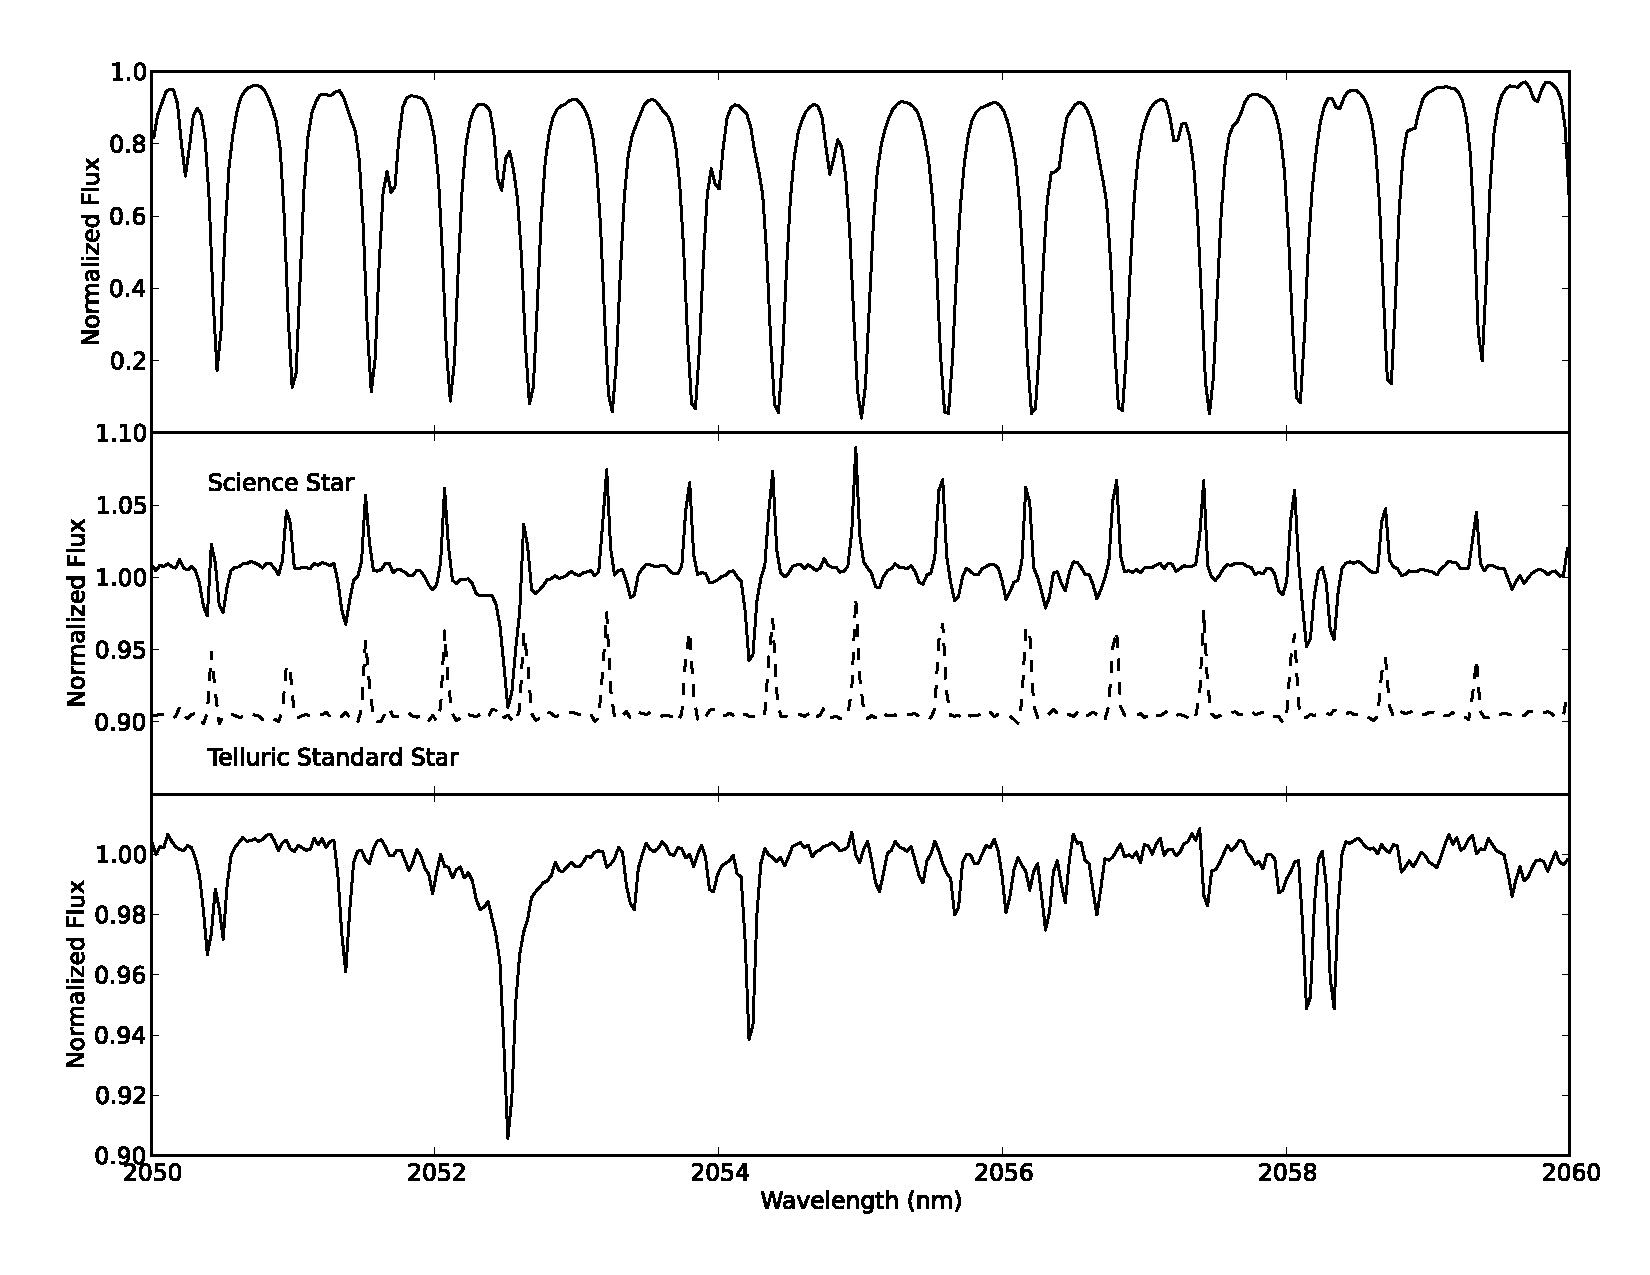
\includegraphics[width=6.5in]{Figures/paper2_fig1.pdf}
  \caption{Telluric Correction process. \emph{Top Panel}: Original
    science star spectrum for a segment in the water band on the blue side of the K band.  \emph{Middle Panel}: Telluric residuals
    after the model fit. The science star residuals are in the upper (solid) line, and
    the standard star residuals are in the lower (dashed) line. The systematic errors we introduced appear like emission lines in both spectra. \emph{Bottom Panel}:
    Result after division of the science star residuals by the
    standard star residuals. The telluric contamination has largely been removed.}
  \label{paper2_fig:tellcorr}
\end{figure}


\begin{figure}[ht]
  \centering
  \includegraphics[width=6.5in]{Figures/paper2_fig2.pdf}
  \caption{\emph{Top Panel}: Individual cross-correlation functions for simulations of HD 189733 with an average S/N = 500, and with complete heat redistribution. The velocities are shifted at each orbital phase such that the cross-correlation function should have a peak at 0 km s$^{-1}$; the planet is only detected in a few of the observations. \emph{Bottom panel}: The total cross-correlation function, after adding the cross-correlation functions for each individual observation. Here the planet is very clearly detected with $6.29 \sigma$ significance.}
  \label{paper2_fig:allcorr}
\end{figure}


\begin{figure}[ht]
  \centering
  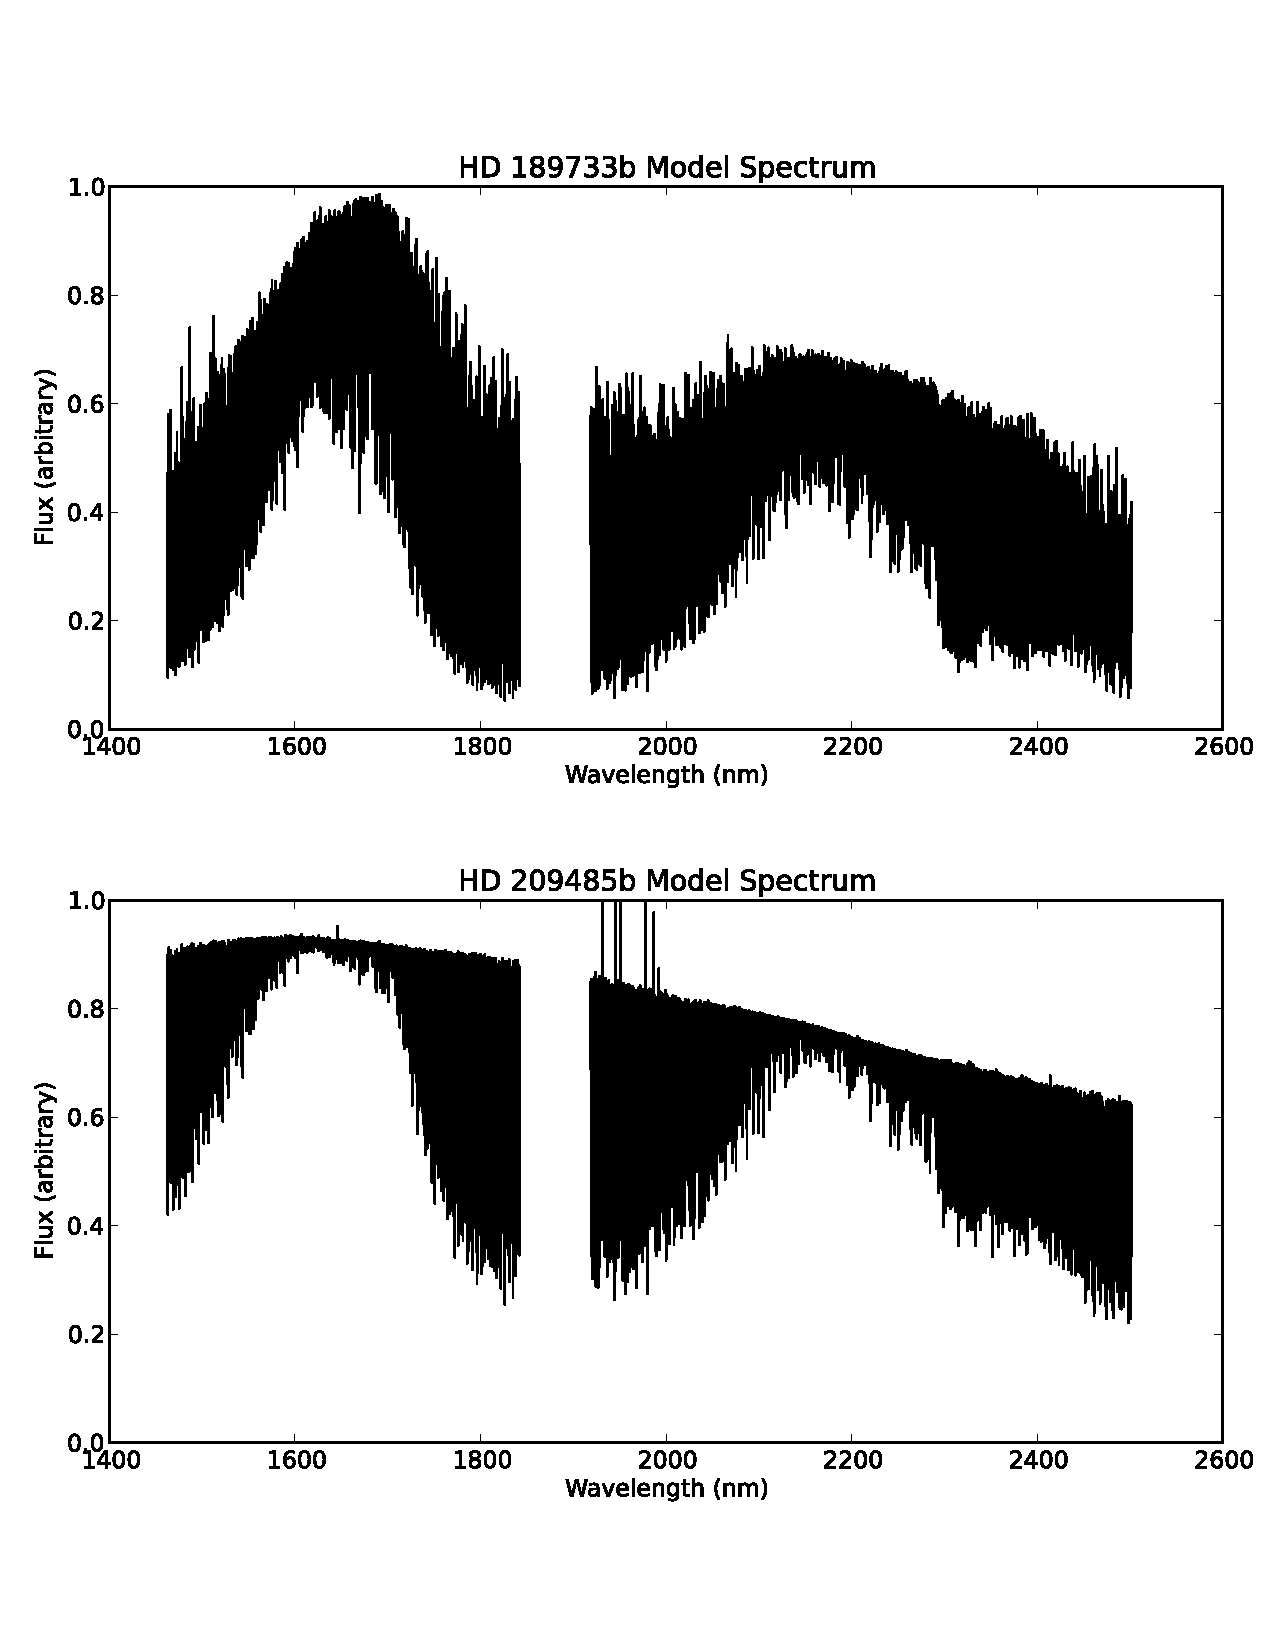
\includegraphics[width=5.5in]{Figures/paper2_fig3.pdf}
  \caption{A comparison of the HD189733 planet model with the HD209458
  planet model. The gap in the middle is is in between the H and K
  spectral windows, where water absorption in the Earth's atmosphere
  blocks most of the incoming light. HD209458b has a thermal inversion
  in its atmosphere, which generates the emission lines near 1950
  nm. HD189733 b is somewhat cooler and has more water, giving its
  spectrum stronger spectral lines.}
  \label{paper2_fig:modelcomp}
\end{figure}


\begin{figure}[ht]
  \centering
  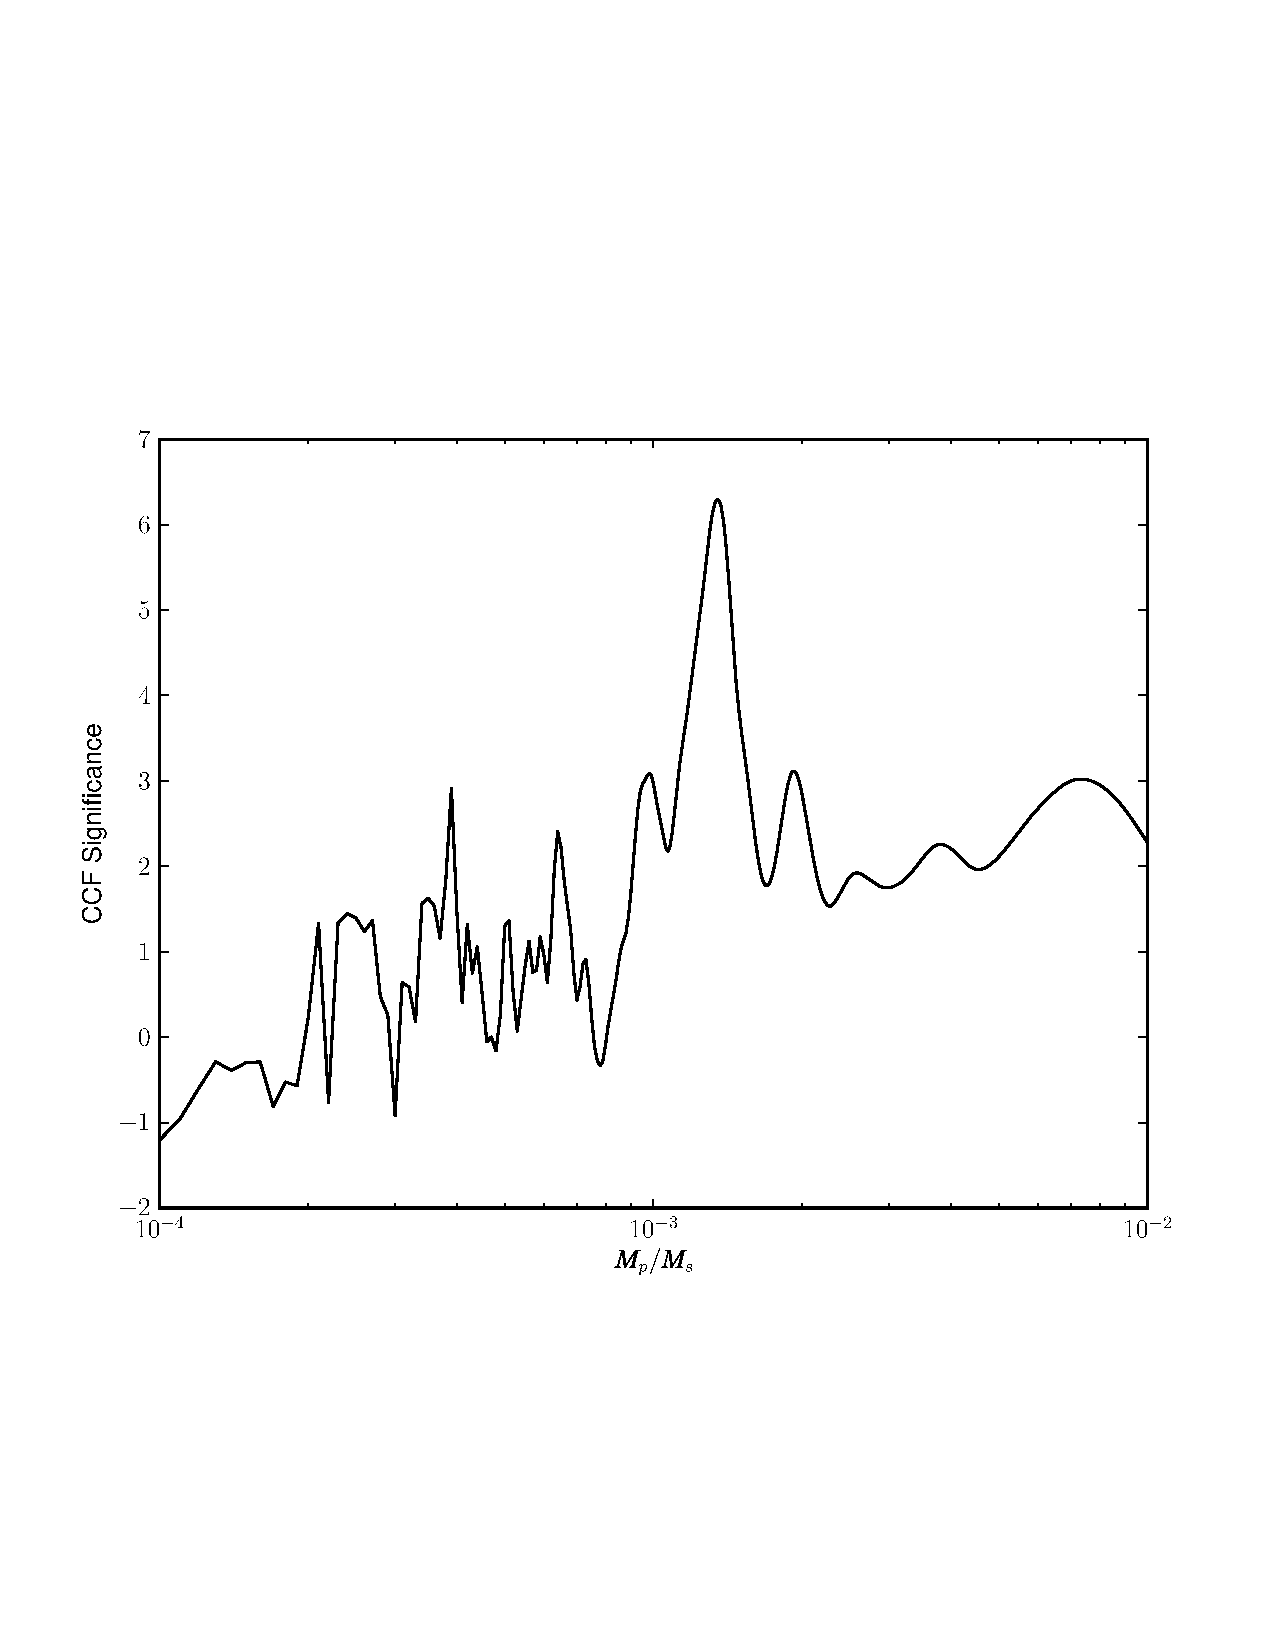
\includegraphics[width=6.5in]{Figures/paper2_fig4.pdf}
  \caption{A summary of the significance of the point at 0 km s$^{-1}$ in the total cross-correlation functions for each of the mass-ratio guesses, for a series of observations of HD 189733 with an average S/N = 500 and complete heat redistribution (the same as in Figure \ref{paper2_fig:allcorr}). The peak in this figure determines the planet to star mass-ratio, and therefore the true planet mass. The width of the peak $1 \sigma$ below its maximum determines the uncertainty in the planet mass.}
  \label{paper2_fig:massratio}
\end{figure}


%%%%%%%%%%%%%%%%%%%%%%%%%%%%%%%%%%%%%%%%%%%%%%%%%%
% Chapter 5  (B-star pilot study)
%%%%%%%%%%%%%%%%%%%%%%%%%%%%%%%%%%%%%%%%%%%%%%%%%%



\chapter{Detection of Low-Mass-ratio Stellar Binary Systems}
\label{chap:pilot}
We now turn back to the variant of the direct spectral detection method originally discussed in Chapter \ref{chap:dsd}, in which the targets are very early-type, rapidly-rotating stars. This chapter was previously published \citep{Gullikson2013_2}. The co-author, Sarah Dodson-Robinson, was my advisor at the time and provided much of the idea for the project.


\section{Introduction}
O- and B-type stars are often found in binary or
multiple systems: \cite{Mason2009} estimate that at least $57\%$ of O-stars are
in spectroscopic multiple systems, and at least $75\%$ are in any type of binary or multiple system.
Yet the multiplicity fraction of high-mass stars may be underestimated due to the difficulty of detecting low-mass secondary stars \citep{Sana2011}.  While the mass-ratio distribution
is reasonably well known for high-mass binaries with mass-ratio $q \equiv M_s/M_p > 0.2$, there are almost no
constraints for low mass-ratio binaries. However, binaries of low mass-ratio are important probes of star formation since they may have
formed in a different way than approximately equal-mass binaries. Here we define low mass-ratios to be 
those with $q < 0.2$, where $M_s$ is the mass of the secondary (lower mass binary component), and $M_p$ 
is the mass of the primary (higher mass binary component). We also use the term ``low-mass'' to 
describe star with $M < 1 M_{\odot}$, and ''high-mass'' to describe stars with $M > 5 
M_{\odot}$


\subsection{Binary Formation in High-Mass Stars}
\label{paper1_sec:formation}
With such a high fraction of high-mass stars found in binary or multiple
systems, any theory of high-mass star formation should be able to
explain the high binary formation rate. There are several mechanisms by
which binary stars may form: fission \citep{Lyttleton1953,
  Lebovitz1974, Lebovitz1984}, in which a molecular core begins
spinning fast enough as it collapses that it splits into two stars;
core fragmentation \citep[see e.g.][]{Boss1979, Boss1986, Bate1995}, in which a collapsing core develops two or more
overdensities which then begin collapsing separately; and disk
fragmentation \citep[see e.g.][]{Kratter2006, Stamatellos2011}, in which the circumstellar disk surrounding the primary
star becomes gravitationally unstable and creates a secondary
star. While the fission scenario was once thought to be important, it
has since fallen out of favor because the viscous dissipation timescale, which would drive a spinning body towards fission, is much longer than the core collapse timescale \citep{Tohline2002} and because hydrodynamic simulations fail to cause
the rotating core to actually split rather than just deform
\citep{Tohline2001}. Both core and disk fragmentation are still
thought to be viable binary formation mechanisms. It is likely that
both mechanisms play a role in shaping the binary mass-ratio and
separation distributions. In the formation of higher-order multiples, it is even possible that both mechanisms operate in the same system.

The primary method of forming binary systems is thought to be core fragmentation. As a molecular cloud
begins isothermally collapsing, its density increases, causing the
Jeans mass to decrease. Thus, an initially Jeans-mass collapsing core
can fragment into smaller objects. Core fragmentation will initially yield binaries with separations
$10 AU < a < 1000 AU$, which may move closer by interacting
with the surrounding gas, a circumbinary disk, or through dynamical
interactions with other nearby stars \citep{BBB2002}. For $\sim 1
M_{\odot}$ primary stars, the observed mass-ratio distribution is well fit by assuming
both components of the binary are chosen randomly from the stellar
initial mass function, and later evolve through
accretion and dynamical interactions \citep{Kroupa2003}. Assuming
independent component masses chosen from the IMF, a binary with a $10 M_{\odot}$ primary would
most often have a $0.1 M_{\odot}$ secondary, giving an initial mass
ratio near $q=0.01$. The unmodified mass-ratio distribution of
high-mass binaries would therefore strongly favor low mass
ratios. However, accretion of high specific angular-momentum gas
from either the collapsing molecular core or
the circumbinary disk will preferentially be captured by the
lower-mass companion, driving the binary mass-ratio toward unity and
decreasing the orbital separation
\citep{Bate2000, BonnellBate2005}. Additionally, dynamical
interactions tend to replace low-mass binary companions with higher-mass ones, or to kick the lower-mass component out to a wide orbit and create a hierarchical triple system. Over time, these processes tend to create high-mass binary systems 
with nearly equal masses and small separations \citep{BBB2002}. Dynamical interactions are most important in dense environments where the probability of stellar encounters is high. Therefore, they are probably more important in dense OB star clusters than in the much looser OB associations, where many B stars are found.

Another potentially important way to form binary systems is disk instability
\citep[see e.g.][]{Kratter2006, Stamatellos2011}. In
this scenario, the fragment forms in an unstable circumstellar disk
with an initial separation of $\sim 100 AU$ and initial mass-ratios
near $q \sim 0.03$, similar to the core fragmentation case
\citep{Kratter2006}. The final mass-ratio is expected to rise, but not
as significantly as in the core fragmentation scenario in which the
fragment can form sooner. Typical mass-ratios near $q \sim 0.1$ are expected, though the picture is far from complete. 
A semi-analytical treatment of embedded protostellar disks by
\cite{Kratter2008} finds that massive stars with $M > 2M_{\odot}$ maintain $0.01 - 0.1
M_{\odot}$ in orbiting fragments after about 2 Myr. \cite{Krumholz2007}
simulate a $100 M_{\odot}$ collapsing core for a much shorter time (20 kyr),
but also find that the disk fragments and that the final fragment mass
ratio is $q \approx 0.1$. However, \cite{Krumholz2009} simulate the same mass core
but start it with a slow solid body rotation instead of a turbulent velocity field and run the model for about twice as long (57 kyr), and find that it leads to a very massive binary ($M_1 + M_2 = 70 \mathrm{M}_{\odot}$) with 
a mass-ratio $q = 0.7$. Work by \cite{Clarke2009} indicates that as
mass is transported inwards onto the star, the outer disk can become unstable at late times. This
instability can lead to a delayed disk fragmentation,
with a fragment mass-ratio in the range $0.1 < q <
0.5$. The simulations by \cite{Clarke2009} were done for a $\sim
1M_{\odot}$ primary star, and the delayed fragmentation occured after
about $10^5$ years. Delayed fragmentation may not be possible in disks surrounding
high-mass stars, as the time at which fragmentation occurs is
comparable to the disk dispersal timescale \citep{Klahr2006}. However,
if it does occur, the similar fragmentation and dispersal timescales suggest that the fragment
would not undergo significant accretion or migration and would leave a
wide binary ($a \approx 100 AU$) with mass-ratio in the range $0.1 < q <
0.5$.

Unfortunately, there are no true binary population synthethis
simulations for high-mass binary systems formed by either mechanism
discussed above. The lack of population synthethis models is driven
by computational issues; a collapsing
cloud that reproduces the stellar mass function \emph{and} generates
enough high-mass stars to meaningfully analyze the binary statistics
would have to be very massive and therefore difficult to
simulate. Disk fragmentation simulations often either stop the
simulation once a fragment forms rather than follow its mass accretion
history \citep[e.g.][]{Boss2011, Krumholz2007}, or lack high enough resolution to follow the secondary very
near the star \citep[e.g.][]{BonnellBate2005}. Fortunately, such models may be in the near future. Realistic simulations of massive collapsing molecular clouds have begun appearing that can meaningfully discuss the multiplicity of low-mass binary systems
\citep{Bate2012, Krumholz2012}. These simulations reproduce the observed increase in multiplicity fraction with primary star mass, but do not yet generate enough high-mass binary system to compare the parameter distributions to observations. Despite the current lack of models, we can draw the general conclusion that disk
fragmentation tends to produce lower-mass companions than core
fragmentation. For this reason, probing the low mass-ratio regime can
provide information on the relative importance of both scenarios in
forming high-mass binary systems, and may help constrain models once
computational power increases.

In addition to binary star formation, disk instability is often invoked as a way
to form planets of a few Jupiter masses orbiting $\sim 1 M_{\odot}$ stars.
While the massive star formation process as a
whole may not simply be a scaled up version of low-mass star
formation \citep{Zinnecker2007}, the process of disk fragmentation may
be. One expects that disks around high-mass stars, with correspondingly higher accretion rates
and more mass, fragment more often than disks around low-mass stars \citep{Boss2011, Boss2006,
  Sally2009, Kratter2006}. Thus, if disk fragmentation plays an important role
in high-mass star formation, it may also play a role in low-mass star
formation by creating $\sim 10M_{Jup}$ planets and substellar companions.



\subsection{Observing low mass-ratio binaries}
\label{paper1_sec:otherobs}
Detection of OB-star binaries with mass-ratio $q \approx 0.1$ or lower is very
difficult, since the ratio of the secondary flux $F_s$ to the primary
flux $F_p$ is $F_s/F_p \sim 10^{-3}$ or lower in the V-band. Imaging surveys
can detect such contrast ratios for wide orbits, but lose sensitivity
as the separation decreases below about $1^{\prime\prime}$
\citep[e.g.][]{Maiz2010}. Spectroscopic binary surveys do well for
short-period systems where a full orbit can be mapped in a reasonable
amount of time, but lose sensitivity for periods greater than about one year
\citep[e.g.][]{Sana2009, Evans2010}. However, low-mass companions ($q \lesssim
0.2$), which induce a small reflex motion on the primary, are very difficult to find with
traditional spectroscopic surveys.

One method to find low-mass companions to late B-type primaries is to
search for high x-ray emission. Stars later than about B3 are not
expected to have strong enough winds to emit X-rays
\citep{Gagne1997}, and stars of earlier type than about A7 do not have
a radiative-convective boundary that can drive a magnetic dynamo and
create an X-ray generating corona \citep{Schmitt1997}. Stars in
between spectral types B4 and A7 with strong X-ray emission are
thought to have young low-mass companions, because the luminosity and
X-ray spectral energy distribution is similar to observed T-Tauri
stars \citep{Huelamo2000}. \cite{Evans2011} use this fact to search fo
low-mass companions to late B-stars in the open cluster Trumpler
16. They find a significant number of 
companions, and set the multiplicity fraction at $39\%$. This value is
a lower limit, but the authors believe that the true value is not much
above $39\%$.  Unfortunately, X-ray imaging is not effective for
primary star spectral types earlier than B3, which are also strong
x-ray emitters \citep{Gagne1997} and will drown out any companions.


\begin{figure*}[t]
  \centering
  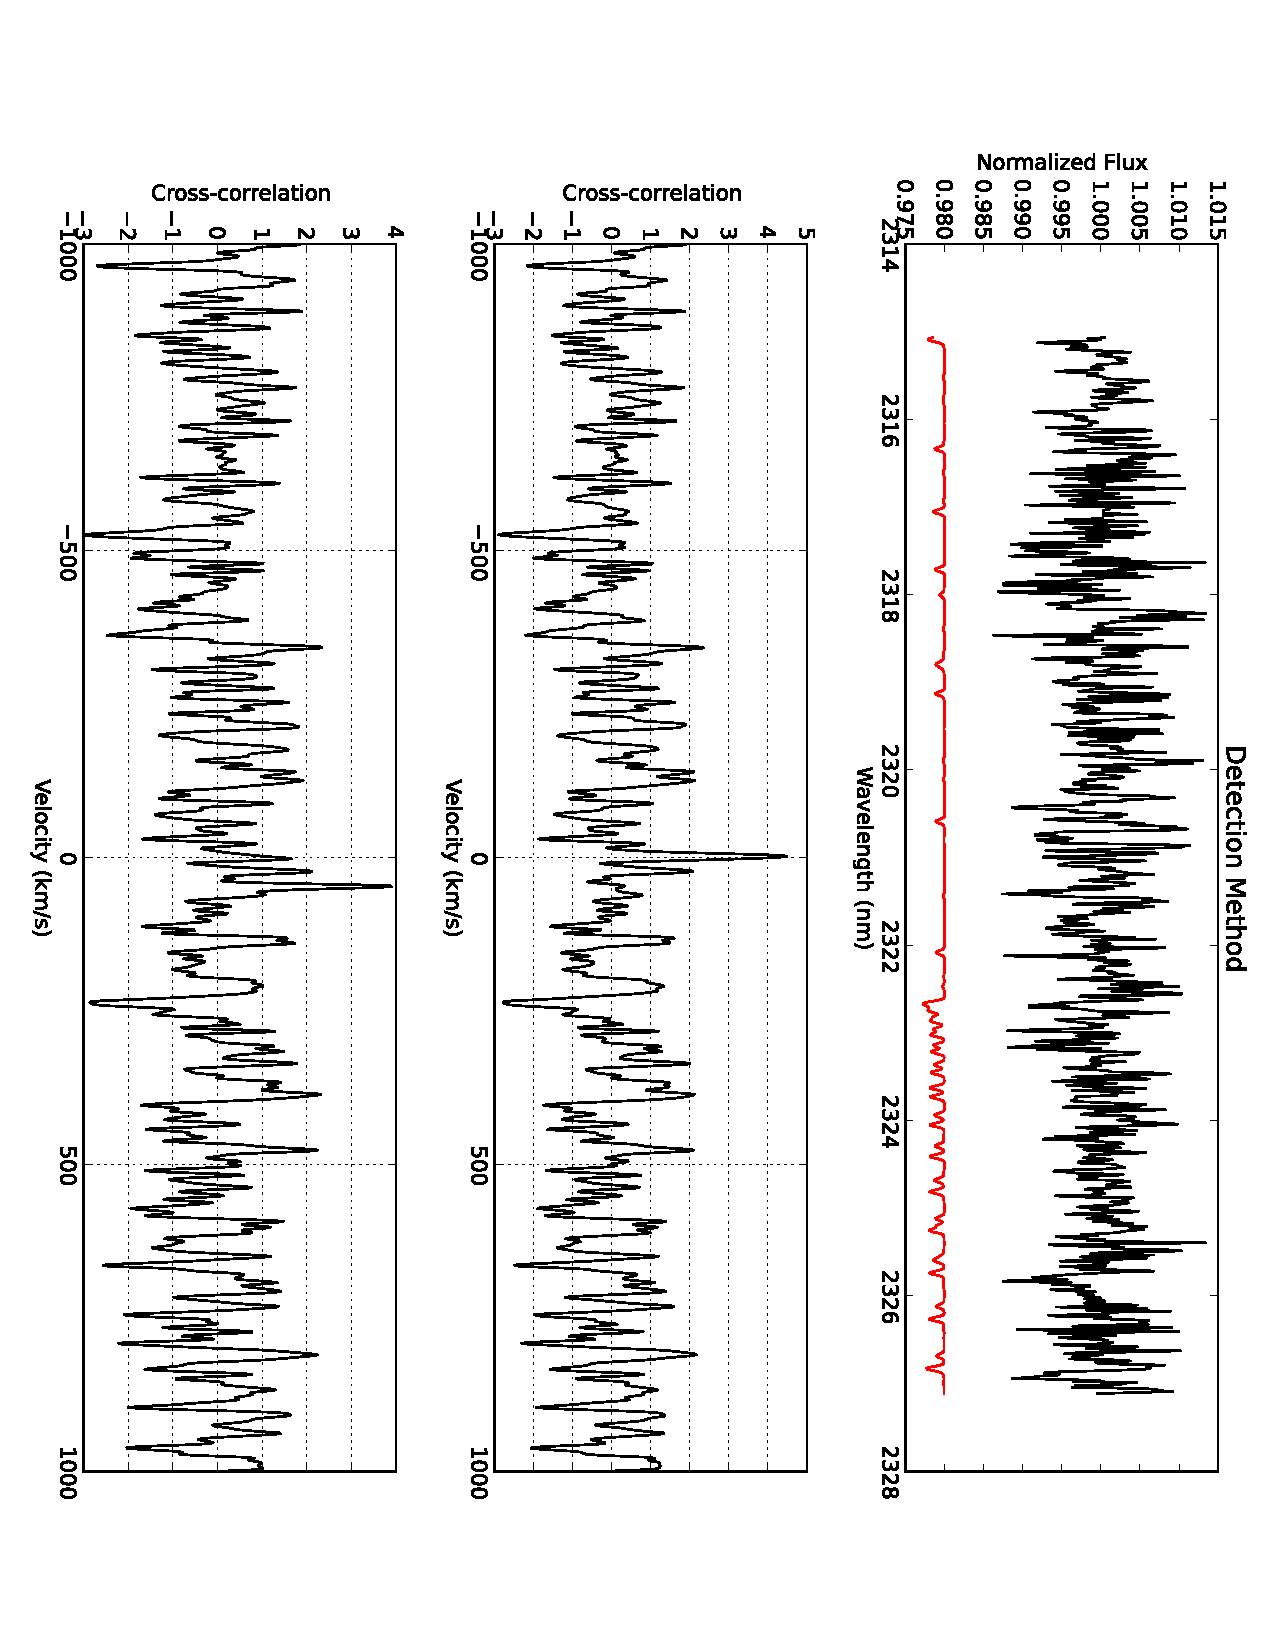
\includegraphics[width=\columnwidth]{Figures/paper1_fig1.pdf}
  \caption{This figure illustrates the approximate flux ratio limit to
  the detection method outlined in section
  \ref{paper1_sec:newmethod}. \emph{Top panel}: Residuals after telluric
  correction (see section \ref{paper1_sec:reduction}) for chip 2 of HIP 80582 are in black, with an
  atmosphere model for an $0.9 M_{\odot}$ star at 50.1 Myr below it in
  red. The flux ratio at this age is $F_s/F_p = 0.0092$. \emph{Middle panel}: The scaled model
  spectrum was added to the telluric residuals, and then the sum was
  cross-correlated with the model. Despite the signal being
  significantly below the noise level, the star was detected at a high
significance. The y axis, in units of the standard deviation of the
cross-correlation function, shows that the significance of the peak is over
$4\sigma$. \emph{Bottom panel}: Same as the middle panel, but the
model spectrum was added to the residuals with a 50 km s$^{-1}$ velocity
offset.}
  \label{paper1_fig:method}
\end{figure*}

In this paper, we introduce a technique that is sensitive to young binary
systems with secondary temperatures $4000$ K $\lesssim T_\mathrm{eff} \lesssim
6000 $K. For early B-type primaries with ages $\sim 15$ Myr, these
temperatures correspond to mass-ratios $q \approx 0.05-0.3$, right
where we expect to see binaries formed by disk instability (see
section \ref{paper1_sec:formation}). Rather
than attempting to detect the reflex motion of the parent
star as in exoplanet searches and SB1 binaries, we attempt to directly
detect the spectrum of the young low-mass companion using high
signal-to-noise, high-resolution data. There is a multitude of archived B-star observations in the near-infrared,
where they are used as telluric standard stars to remove the absorption spectrum of the Earth's atmosphere (telluric
lines). This method is equally sensitive to all separations within the point spread function, which is dominated by the seeing since the adaptive optics are not used in telluric standard star observations. A typical seeing of $\sim 0.8''$ corresponds to up to $\sim 900$ AU for targets within a few kpc. In this paper, we describe a search for young F5-K9 type companions in archived VLT/CRIRES spectra of 34 early B-type stars.

In section \ref{paper1_sec:newmethod} we describe our detection method in 
more detail. Section \ref{paper1_sec:sample} describes the B-star sample we use in this work.
Section \ref{paper1_sec:reduction} contains the data reduction and telluric correction methods. 
We summarize our results in section \ref{paper1_sec:results}. We examine the
completeness of our sample in section \ref{paper1_sec:completeness} and put
limits on the multiplicity fraction as a function of mass-ratio in
section \ref{paper1_sec:multiplicity}. Finally, we present our conclusions about the prevalence of low mass-ratio companions to early B-type stars and discuss how our results constrain star formation mechanisms in Section \ref{paper1_sec:conclusions}.


\section{Direct Spectral Detection Method}
\label{paper1_sec:newmethod}

We describe here our method to detect the emission from an
approximately solar-mass star orbiting an early B-type star, which we
will hereafter call the direct spectral detection method. The basis of
this method is to cross-correlate a high signal-to-noise ratio B-star
spectrum with a synthetic F,G, or K star spectrum. If a low-mass star
with such a spectrum is orbiting the B-star, we expect to find a peak
in the cross-correlation function at the radial velocity corresponding to
the low-mass star's motion. A peak in the cross-correlation
function should appear even if the
flux from the low-mass star is comparable to or even slightly less than the noise level in the
spectrum. Figure \ref{paper1_fig:method} illustrates the approximately limiting
case for the flux ratio. The top panel shows a fully reduced CRIRES spectrum of HIP 108975 (see section \ref{paper1_sec:reduction}) with a model spectrum for an $0.9 M_{\odot}$ star at a realistic flux ratio below it. We used
evolutionary tracks published by \cite{Landin2008} to evolve the secondary star
to 50.1 Myr, the age of the system \citep{Tetzlaff2010}, in order to determine the flux
ratio between the primary and secondary. The secondary star model was then added to
the telluric-corrected B-star spectrum at two different velocities. It is clear that the model spectrum has an amplitude much smaller
than the noise.  Nonetheless, the bottom two panels show that a cross-correlation will
have a peak with high significance at the velocity of the secondary star.


\begin{figure*}[t]
  \centering
  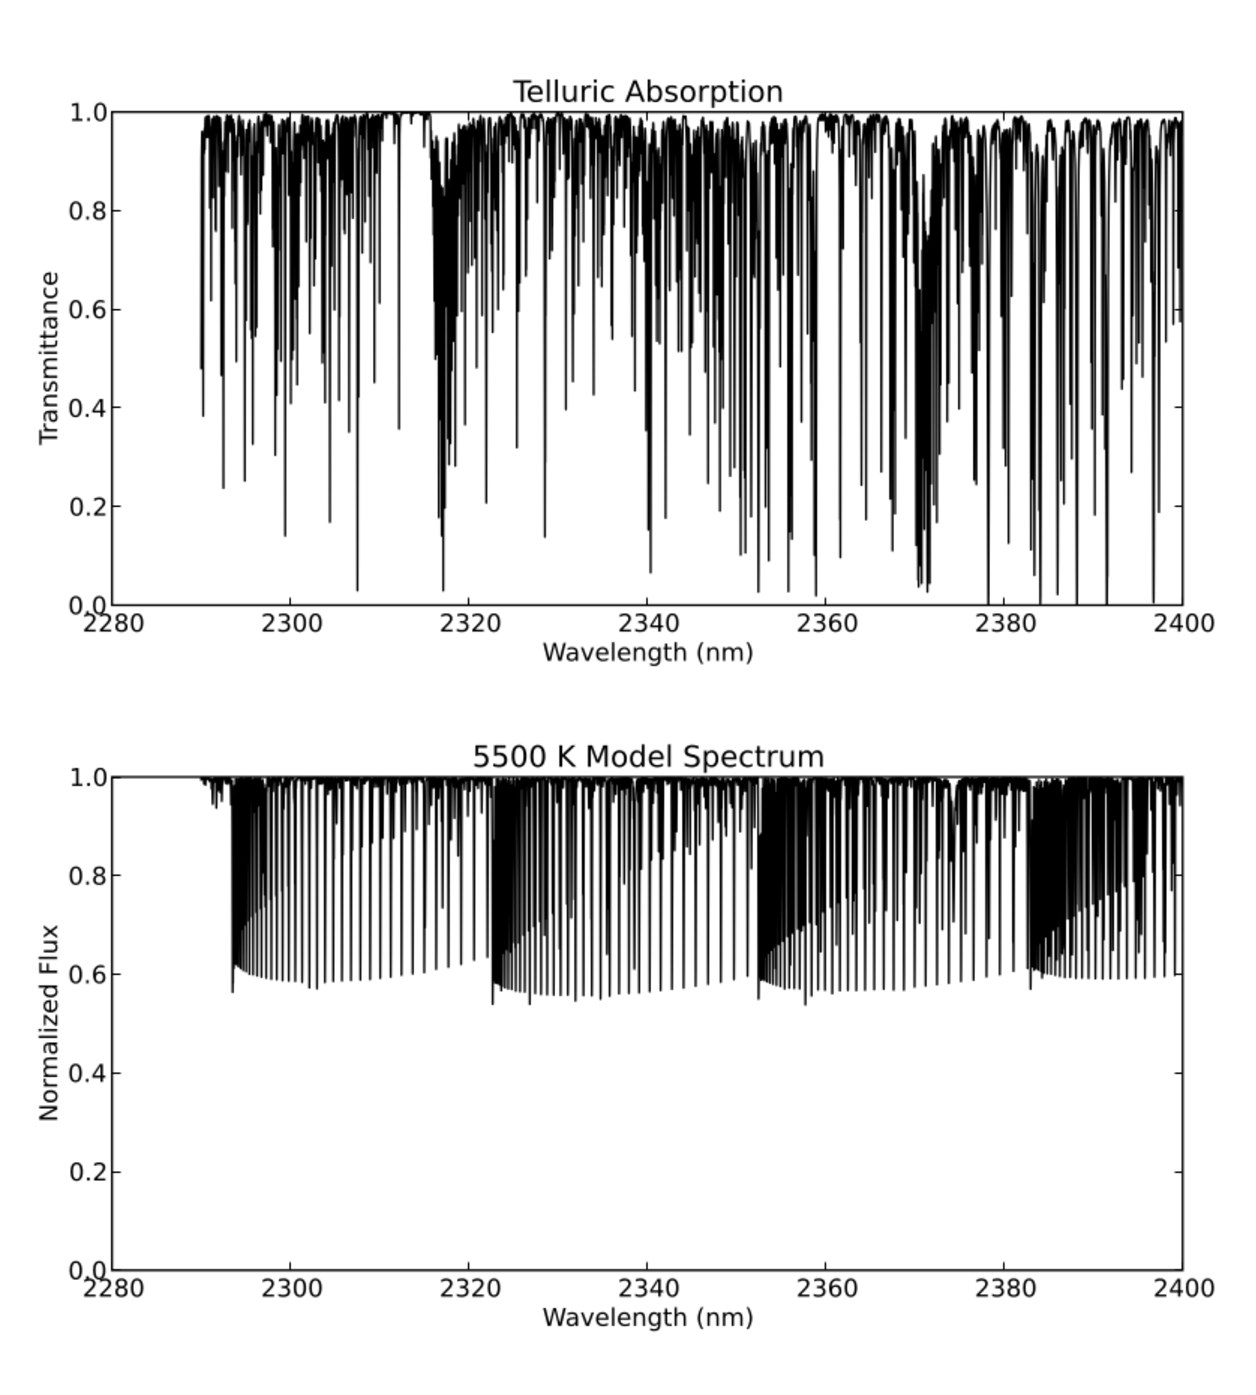
\includegraphics[width=\columnwidth]{Figures/paper1_fig2.pdf}
  \caption{\emph{Top panel}: The telluric spectrum (absorption due to Earth's
    atmosphere) in the wavelength range from $2290-2400$ nm. Most of the lines are
    from CH$_4$, with a few H$_2$O lines appearing in the right
    half. \emph{Bottom panel}: The model spectrum of a 5500 K star
    with $\log (g) = 4.0$ and solar metallicity. Note that the line density of telluric
    lines is comparable to or greater than that of the star model, and many of the
    telluric lines are stronger than the stellar lines.}
  \label{paper1_fig:telluric}
\end{figure*}

A careful choice of the wavelength region is critical for the direct spectral 
detection method. First, we want a wavelength region where the B-star spectrum
is mostly continuum (i.e. very few spectral lines). Since B-stars have few spectral lines, it is
easy to find a such a spectral region. Secondly, we want a region where the low-mass star
would have many closely spaced, strong lines. The more lines there are
in the low-mass star, the stronger the peak will be in the
cross-correlation function. Finally, we want a spectral region where the
flux ratio between the low-mass and the high-mass star is maximized.
It is not helpful to go much redder than a few microns for  
companions with $T>4000$K, because both the high-mass and
the low-mass star are firmly in the Rayleigh-Jeans limit by this
point, where the flux ratio is approximately constant. For this project,
we choose wavelengths from $2300-2400$ nm, which is the CO $\Delta\nu = 0-2$
bandhead in the low-mass star. 

There is both a lower and upper mass detection
limit. Secondary stars that are too cool will be too faint, and any
signal will be lost in the noise. Additionally, a more massive (and
hotter) primary star will decrease the flux ratio, and push the lower
mass limit up. On the other end, secondary
stars that are too hot will dissociate CO, destroying the bandhead
that we are looking for. The temperature and size of the secondary star will
depend on its age as well as its mass since it will still be
evolving towards the Main Sequence during the lifetime of the
B-star. The exact mass sensitivity will thus depend on the age,
primary star mass, and signal-to-noise ratio of the system being observed. 

The detector resolution is also important for the direct spectral detection
method. Deeper lines, providing more contrast from the
continuum, are easier to detect than broad, shallow lines. In
addition, narrow spectral lines will result in a stronger, narrower peak in the
cross-correlation function, which is most sensitive to the steep line
edges. Therefore, we want the spectral lines in the low-mass companion
to be as deep and narrow as possible. The intrinsic width of CO bandhead lines is
roughly 5-7 km s$^{-1}$. In order for the observed line width to be this
small, we need the resolution of the instrument to be $R =
\lambda/\Delta \lambda \gtrsim 50000$. 



There are two main difficulties with the direct spectral detection method: 
telluric line removal and the low flux ratio between the primary and secondary
star. Figure \ref{paper1_fig:telluric} shows the transmittance through the
Earth's atmosphere (the telluric spectrum) in the wavelength range we
are interested in. Most of the spectral lines are from methane, with a
few deep water lines towards the red end
of the range shown (See section \ref{paper1_sec:reduction} for details on the
telluric line removal). The low flux ratio makes the telluric
contamination especially troublesome, since the telluric lines are
stronger than the lines in the companion star spectrum. The flux ratio of $F_s/F_p
\sim10^{-2}$ effectively sets a lower limit on the signal-to-noise
ratio for which the direct spectral detection method is possible. 
Any flux coming from a low-mass star will be completely buried
in the Poisson noise for spectra with SNR $\ll100$. Removal of the 
telluric contamination will add more noise to the spectrum, so a spectrum
should have SNR of a few hundred \emph{before telluric line removal}
to have a good chance of detecting a companion.



\section{Star Sample}
\label{paper1_sec:sample}
B-type stars are commonly used in the near-IR as telluric
standard stars. Astronomers will observe their science targets, and
then move to a B-type star. Since B-type stars have few
spectral lines relative to cooler stars, most of the observed
spectral lines will be from the absorption of Earth's atmosphere
(telluric absorption). Therefore, these stars provide an empirical
estimate of the telluric spectrum; division of the science spectrum by
the normalized standard star spectrum will mostly remove the telluric
lines. 

Since B-type stars are commonly used as above, there are
many high signal-to-noise ratio (S/N $\gtrsim 100$)
observations of such stars in archived data. We used the VLT/CRIRES
archive in this project. CRIRES is a high
resolution ($R = \lambda / \Delta \lambda \approx 100000$) infrared
spectrograph on the VLT at Paranal Observatory. The detector consists of four
1024x512 ccd chips that are mosaiced end-to-end, and
the spectrum falls across them. There are several wavelength settings
available, which determine what parts of the spectrum fall on each 
chip. For wavelength settings in the CO
bandhead near 2300 nm, each chip will hold rougly 10 nm of spectrum
with roughly 1-2 nm gaps between the chips.

To generate the sample, we started with all single, main sequence B0-B5 stars 
with CRIRES observations from 2300-2400 nm. We then excluded any shell stars, which have circumstellar disks \citep{Porter2003} that may create
false positives. Table \ref{paper1_tab:sample} shows the complete sample used in this
project. The spectral types and ages were obtained from a catalog of nearby
young stars \citep{Tetzlaff2010}. The one exception is HIP 97611, which was
not in \cite{Tetzlaff2010}. For this star, the age was taken from
\cite{Westin1985} and the spectral type from the Simbad database\footnote{\url{http://simbad.u-strasbg.fr/simbad/}}
. The distances to all stars were
determined from parallaxes given in the Simbad database. The maximum
separation column estimates the approximate maximum separation of the binary
orbit we are sensitive to, assuming a seeing of 0.8'' which is typical of
Paranal Observatory. The median of the maximum separations to which we are sensitive is 124
AU.  The final column gives the number of distinct observations of the
star. We count all nodding positions taken on a given night with the same 
detector wavelength setting as one observation.


\begin{figure*}[ht]
  \centering
  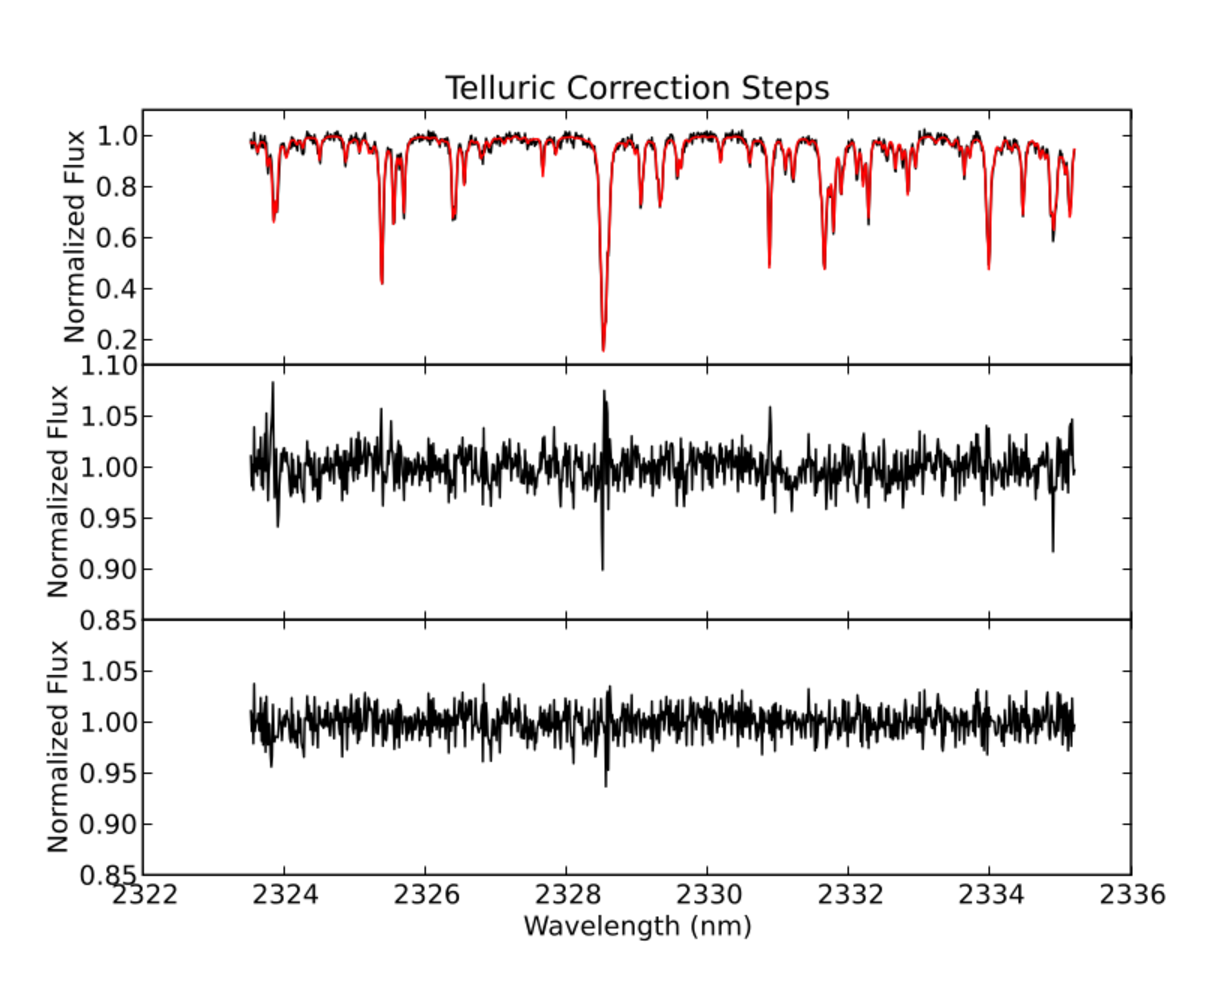
\includegraphics[width=\columnwidth]{Figures/paper1_fig3.pdf}
  \caption{The telluric correction steps for chip three of CRIRES
    wavelength setting $\lambda_{ref} = 2329.3$ nm. \emph{Top panel:}
    Normalized spectrum (black), with the best-fit telluric model
    (red). \emph{Middle panel:} Residuals after dividing the observed
    spectrum by the telluric model. Note the large spikes near
    $2328.5$, $2331$, and $2335$ nm. \emph{Bottom panel:} Correction
    after fitting the large residuals to Gaussians. }
  \label{correctionsteps}
\end{figure*}



\section{Data Reduction and Telluric Correction}
\label{paper1_sec:reduction}
The data reduction was done using standard methods in
IRAF\footnote{IRAF is distributed by the National Optical Astronomy Observatories,
    which are operated by the Association of Universities for Research
    in Astronomy, Inc., under cooperative agreement with the National
    Science Foundation.}. All observations were taken in an AB or ABBA nodding
pattern. For each set of AB nods, A-B and B-A frames were made to
remove any atmospheric emission lines and dark current. The resulting
difference images were then treated to a quadratic nonlinearity correction, using
coefficients made available by the CRIRES
team%\footnote{\url{http://www.eso.org/observing/dfo/quality/CRIRES/pipeline/pipe_calib.html}}. 
The corrected frames were then divided by a normalized flat-field. Due
to the slit curvature, the spectrum can shift by up to a pixel in
the dispersion direction between the A and B nod positions. Therefore,
combining the 2D frames before extraction can reduce the spectral
resolution and affect the line shapes. For this reason, we
combined the nodding positions only after the wavelength
calibration and telluric correction. Each nod position was extracted using the 
optimal algorithm in the apall task in IRAF. The spectra were wavelength 
calibrated using a model telluric
spectrum generated with the atmospheric modeling code
LBLRTM%\footnote{\url{http://www.rtweb.aer.com/lblrtm_description.html}}
\citep{Clough2005}.


For telluric correction, we used a similar procedure to the one outlined by
\cite{Seifahrt2011}. The atmosphere modeling code
LBLRTM was used to generate a synthetic telluric
absorption spectrum. The abundances of water,
methane, and carbon monoxide were fit using a Python implementation of
a Levenberg-Marquardt nonlinear least squares fitting algorithm. The
Levenberg-Marquardt fit also refined the wavelength solution to the
telluric model, fit the continuum, and fit the resolution of the
spectrograph with a Gaussian profile. The FWHM of the profile was the
only free parameter in the resolution fit.

The LBLRTM code expects a model atmosphere, which contains the
temperature, pressure, and abundance of 30 molecules as a
function of atmospheric height. For the majority of molecular species,
we used a mid-latitude nighttime
MIPAS\footnote{\url{http://www-atm.physics.ox.ac.uk/RFM/atm/} }
profile, which provides the temperature, pressure, and abundances of
various molecules in 1 km intervals from sea level to 120 km. The
low-altitude ($z \lesssim 30$ km)
temperature, pressure \citep{Kerber2010}, and humidity
\citep{Chac2010} profiles were obtained from radiosonde data taken from Paranal Observatory.


The LBLRTM atmospheric modeling code comes with a molecular line list
based on the HITRAN 2008 database \citep{Rothman2009}, with a few
molecules individually updated. Since none of these updates were
relevant for the wavelength range from $2300 - 2400$ nm, we in
essence used the stock HITRAN 2008 database. However,
in the process of modeling, we found several water and methane lines
that were consistently under- or over-fit. For these cases, we
manually adjusted the line strengths in the database. The line
strengths were fit visually and should not be considered rigourous new line strengths. Table \ref{paper1_tab:linelist}
summarizes these changes.


In some of the 2007 data, the first chip was not well illuminated
by the flatfield lamp. This introduced an unphysical continuum shape
in the data and made the resulting model fit very poor. For these
cases, we ignored the first chip in further analysis. In addition,
the fourth chip has several bad pixels on the left edge and a streak
down the middle. None of the telluric model fits were very good on
this chip, and so we have ignored it completely in our analysis.

After the observed spectrum was fit, we found that the residuals still
contained large spikes, even on the good detector chips. These spikes
can come from a variety of sources. For the deepest lines, simple
Poisson noise can create large residuals when dividing by the telluric
model. In addition, a poorly fit continuum may cause the model to over- or under-estimate
the abundance of a given molecule. This can be especially troublesome
for water lines, for which only a few exist in the wavelength region we
are investigating. If a strong water line is near the edge of the
chip, where the continuum is usually least certain, the best-fit water
abundance may be skewed and cause none of the water lines to be well fit. We do know
that large residuals are \emph{not} coming from the spectrum of a
low-mass star, due to the expected flux ratio between the primary and
secondary, $F_s/F_p \sim10^{-2}$. Any residuals with amplitude greater than 
$1\%$ of the continuum level come from uncorrected telluric lines,
cosmic rays, or bad pixels. 

In order to minimize these spikes, we performed a second fit to any
residuals significantly above the continuum noise level. To make sure
we were not fitting away any low-mass star lines, we only corrected
spikes whose amplitude was greater than $5\%$ of the continuum level. In this
second fit, we first attempted to fit a Gaussian to each spike. If the
spike was well fit by a Gaussian, we divided the residuals by the fit.
If not, we
simply masked out the line core, so that it would not affect the
cross-correlation in later analysis (see section \ref{paper1_sec:newmethod}). Figure
\ref{correctionsteps} shows the steps involved in the telluric
correction. Notice that the secondary correction removes the
large residuals, while leaving the rest of the spectrum
unaffected. 



The telluric correction described above usually reduced any telluric
lines to near the Poisson noise level in the spectrum, which is the best a
fitting routine can do. To search for any systematic errors in the
telluric correction, we added all spectra of each wavelength setting
together to make a series of master telluric residual spectra. These
master spectra had less random noise than any individual observation, and therefore we were
immediately able to see whether some telluric lines are systematically
under- or over-fit. We found that for wavelength settings with at
least ten spectra in our sample, dividing the corrected spectra by
this systematic telluric residual template increased the sensitivity
to companions. We did not make this final correction for
wavelength settings with fewer than ten individual spectra in our sample.



\section{Results}
\label{paper1_sec:results}
Each telluric residual spectrum was cross-correlated against a suite of model atmospheres
generated by the Phoenix stellar atmosphere code \citep{Hauschildt1999}. All model spectra had solar metallicity. The effective
temperatures ranged from $3000-7200$ K, in 100K intervals. We used
several surface gravities based on the stellar temperature. For the
model secondary stars with $3000 < T_\mathrm{eff} < 3600$, which would
have to be very young (and large) to be detectable, we used a $\log (g) = 3.5$. For the secondaries with
$3600 < T_\mathrm{eff} < 6500$, we used $\log (g) = 4.0$. Finally, we used
$\log (g) = 4.5$ for $T_\mathrm{eff} > 6500$, which can be detected
closer to the Main Sequence. We found that the surface gravity has only a very small
effect on the cross-correlation, which is more sensitive to the line
position than its precise width or depth. We
compiled a list of all cross-correlations that show a single peak with
at least $3\sigma$ significance. For a given telluric-corrected residual
spectrum, several model atmospheres may generate a significant peak at
the same velocity. This is because the model spectra of two stars
differing by only a few hundred kelvin are not very different. To keep from
counting peaks twice, we only counted the cross-correlation that
resulted in the most significant peak at a given velocity. We then attempted to
reject spurious peaks caused by the noise or incomplete telluric line
removal in a multi-stage process.

The first rejection stage was done by identifying peaks in the
cross-correlation caused by telluric residuals. To do this, we
cross-correlated a spectrum uncorrected for telluric absorption with
the same suite of model atmospheres as we used for the corrected
spectra (see above). We did these cross-correlations for one observation of each wavelength
setting. The cross-correlation of uncorrected spectra with model-atmosphere spectra generated a series of cross-correlations with peaks
arising exclusively from telluric lines. We visually compared all
of the binary candidate signals with these telluric
cross-correlations. If the dominant cross-correlation peak was at the
same velocity and had a similar width as a peak in the telluric
cross-correlation function corresponding to the same wavelength
setting and secondary model temperature, we assumed that the peak was caused by incomplete
telluric removal and rejected the candidate. There were several
cross-correlations with peaks at the same location as a telluric peak,
but with a different width. In these cases, we marked the candidate as
probably coming from incomplete telluric correction, but did not
reject the candidate.



\begin{figure*}[ht]
  \centering
  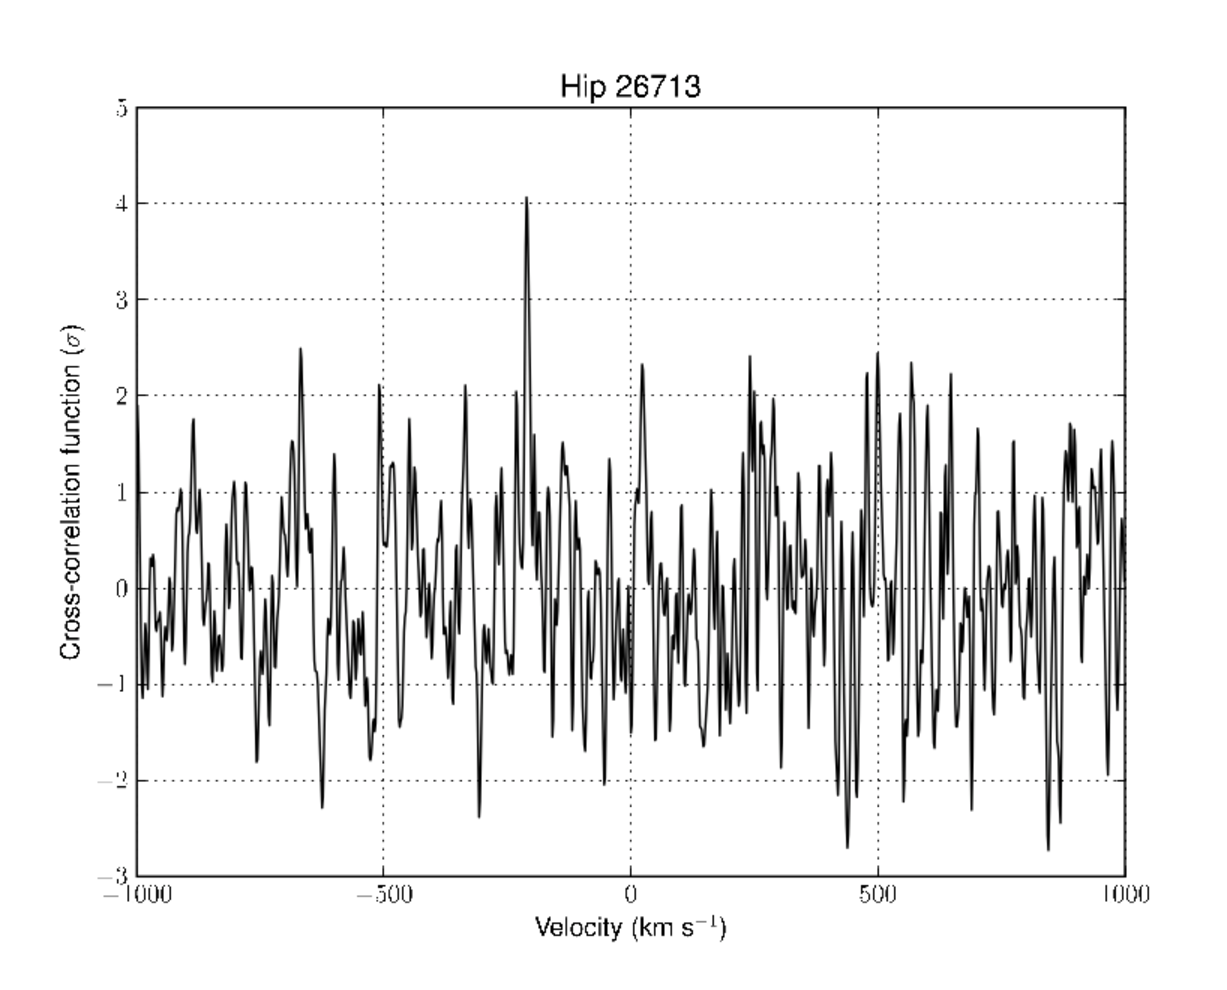
\includegraphics[width=\columnwidth]{Figures/paper1_fig4.pdf}
  \caption{Cross-correlation for HIP 26713, using a 5600 K star model spectrum as template. The y-axis is in units of
    the standard deviation of the cross-correlation function. The peak is very near the maximum velocity of $|v_\mathrm{max}| = 256$ km s$^{-1}$, assuming a circular orbit (see equation \ref{paper1_eqn:vmax}). The likelihood of observing the system nearly edge on and at a quadrature point, so that $|v| \sim |v_\mathrm{max}|$, is $p \approx 0.01$. However, it is possible that the system has an eccentric orbit, effectively increasing $|v_\mathrm{max}|$.}
  \label{paper1_fig:hip26713}
\end{figure*}

Next, we determined whether the signal-to-noise ratio and telluric line removal in a given observation would allow us to detect the candidate companion star.
To do this, we added a model atmosphere with the
same temperature as the candidate to the telluric-corrected spectrum at 17 different radial
velocities ranging from -400 to 400 km s$^{-1}$. We do not expect to see any
peaks from real companions with $|v| > 400$ km s$^{-1}$, the approximate
radial velocity of a $1 M_{\odot}$ star orbiting a $10 M_{\odot}$ star
such that the stellar surfaces are in contact. The flux ratio of the model atmosphere to the primary was obtained by
interpolating pre-main-sequence evolutionary tracks from
\cite{Landin2008} at the age of the system, as well at age$\pm
\sigma_{age}$. The primary star ages for our sample are given in Table
\ref{paper1_tab:sample}. We cross-correlated each of these semi-synthetic
spectra against the model spectrum; if the largest
peak was at the correct velocity, we counted the star as
detected. If the star was not detected in the sensitivity
analysis at least $50\%$ of the time, we rejected the candidate.
The significance of the correct peak in the cross-correlation 
function can vary greatly, depending on where the stellar spectrum falls in 
relation to the telluric line residuals. Therefore, we cannot usually reject a peak
based solely on its significance.

We then visually inspected the remaining candidate cross-correlations,
picking out those with a single dominant peak with $|v_r| < v_\mathrm{max}$
where $v_\mathrm{max}$ is the maximum possible radial velocity for a star of
temperature $T_\mathrm{sec}$ to be orbiting a hotter star of temperature
$T_\mathrm{prim}$ with a semimajor axis $a$. Assuming a circular orbit,
$v_\mathrm{max}$ is given by

\begin{equation}
v_\mathrm{max} = \sqrt{\frac{2G(M_\mathrm{prim} + M_\mathrm{sec})}{R_\mathrm{prim}}} \cdot \frac{T_\mathrm{sec}}{T_\mathrm{prim}}
\label{paper1_eqn:vmax}
\end{equation}

where $M_\mathrm{prim}$ and $M_\mathrm{sec}$ are the masses of the primary and
secondary stars, respectively, and $R_\mathrm{prim}$ is the radius of the
primary star. The primary masses are given in \cite{Tetzlaff2010}, while
the radii and primary star temperatures were estimated from spectral type relations given in
\cite{CarrollOstlie}. An eccentric orbit could have a larger maximum velocity than
that estimated by equation \ref{paper1_eqn:vmax}, if the orbit was oriented
such that the the secondary star was moving directly towards or away from earth at or near
periastron. A star in an eccentric orbit cannot get so close to the
primary that they touch, and its \emph{average} distance must still be
far enough to allow for the observed secondary star temperature. These
conditions lead to a maximum eccentricity, given by

\begin{equation}
e_\mathrm{max} = 1 - \frac{v_\mathrm{max}^2 (R_\mathrm{prim} + R_\mathrm{sec})}{G(M_\mathrm{prim} + M_\mathrm{sec})}
\label{paper1_eqn:emax}
\end{equation}

where $R_\mathrm{prim} $ and $R_\mathrm{sec}$ are the radii of the primary
and secondary stars, respectively, and $v_\mathrm{max}$ is the maximum
circular velocity given by equation \ref{paper1_eqn:vmax}. Typical values
give $e_\mathrm{max} \approx 0.6$. Eccentricities near this value could
allow for velocities significantly greater than $v_\mathrm{max}$ given by
equation \ref{paper1_eqn:vmax}.

The above analysis is summarized in Table \ref{paper1_tab:rejection}. There
are two binary candidate systems that we have not been able to reject.
 For both of these, we checked what other observations the candidate
star had within the CO bandhead spectral region ($2300-2400$ nm). The analysis of each
of these stars is done separately below.

%\newpage


\subsection{HIP 26713}
The cross-correlation for this candidate is shown in figure
\ref{paper1_fig:hip26713}. The strong peak at -220 km s$^{-1}$ has a
significance just over $4\sigma$, and corresponds to a 5600 K star
model. A sensitivity analysis (Table \ref{paper1_tab:rejection}, step 2) gives a median peak significance of $\sim 6\sigma$
with a large ($\sim 2\sigma$) spread. Due to the large spread, we cannot reject
the peak based on the observed significance.

The candidate radial velocity amplitude of 220 km s$^{-1}$ is very near the upper limit 
given by equation \ref{paper1_eqn:vmax} of 256 km s$^{-1}$. If this candidate is a real binary companion, it
must have been observed very near its radial velocity maximum and the orbital inclination must be very
near edge-on. Assuming a circular orbit and equal probabilities
of observing any given phase or inclination, the probability of this
occuring for this system is $\sim 0.01$. However, the probability for one system in our entire sample to be caught with this chance alignment rises to $0.14$.  In addition, we cannot discount the
possibility of an eccentric orbit leading to a higher value of $v_\mathrm{max}$ than estimated by equation \ref{paper1_eqn:vmax}. Without more data, we can neither confirm nor disprove the existence of a companion star orbiting HIP 26713.
  
If HIP 26713 is a true binary system, evolutionary tracks by \cite
{Landin2008} give a secondary star mass of $1.6 \pm 0.2 M_{\odot}$. 
The mass of the primary star is $9.4 \pm 0.2 M_{\odot}$ \citep
{Tetzlaff2010}, giving a mass-ratio of $q = 0.17 \pm 0.02$. For a circular orbit, the corresponds to an orbital period of 10.0 days. If the companion star is on an eccentric orbit, its true period would be longer than this.

\begin{figure*}[ht]
  \centering
  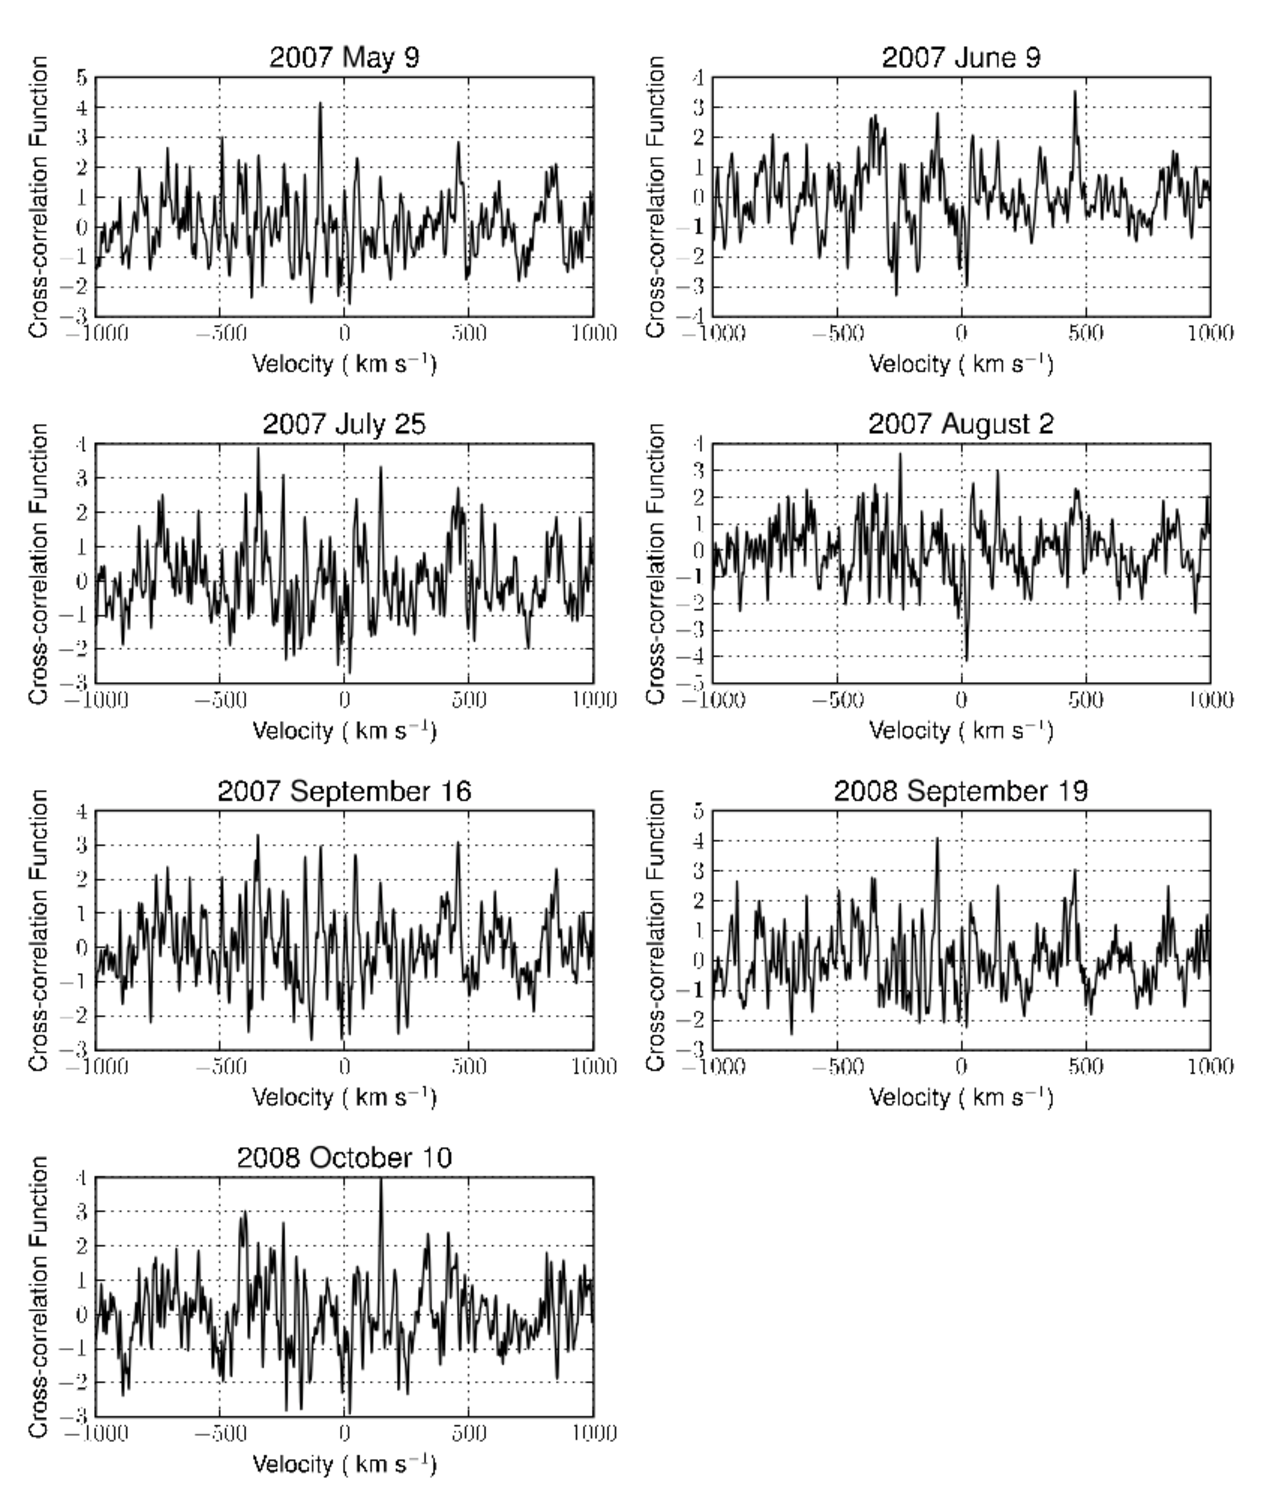
\includegraphics[width=5.7in]{Figures/paper1_fig5.pdf}
  \caption{Cross-correlations for HIP 92855, for all dates observed. A 6100 K star model spectrum is used as the template for each cross-correlation. The y-axis is in units of
    the standard deviation of the cross-correlation function. A single strong peak is seen in the
    cross-correlations from 2007 May 9, 2007 August 2, 2008 September
    19, and 2008 October 10. The reasonably strong peak on 2007 June 9 is identified
  as probably arising from imperfect telluric line removal or random noise, since it
  has $v>v_\mathrm{max}$ given by equation \ref{paper1_eqn:vmax}.}
  \label{paper1_fig:hip92855}
\end{figure*}




\subsection{HIP 92855}
\label{paper1_sec:hip92855}
There were seven observations of HIP 92855 on different dates, all with the 2336 nm
wavelength setting. The cross-correlations for four of the observation dates show
a single strong peak when using a 6100K model star as template. Figure
\ref{paper1_fig:hip92855} shows the cross-correlations of the
telluric-corrected spectra with a 6100K model for all of the
observations. Table \ref{paper1_tab:hip92855} summarizes the sensitivity and
cross-correlation significance. The detection rate is the fraction of the 17
radial velocities between -400 and 400 km s$^{-1}$ that were correctly detected in the sensitivity
analysis (Table \ref{paper1_tab:rejection}, step 2). The variation in detection rate is due to the different
signal-to-noise levels and telluric line corrections in the observations
at different dates. The expected significance is the median significance of
the radial velocities which were detected in the sensitivity analysis, in units of
the standard deviation of the cross-correlation function. The observed
significance and velocity are for the observed peaks. The velocities in Table \ref{paper1_tab:hip92855} are corrected for
the barycentric motion and the known systematic radial velocity of HIP 92855,
while those in Figure \ref{paper1_fig:hip92855} are not.



As Table \ref{paper1_tab:hip92855} shows, a 6100K star orbiting HIP 92855 is at
the limit of detectability with the direct spectral detection
method. With the exception of the observation on 2007 September 16, the
cross-correlations for the dates with the highest detection rates have
a single large peak. We consider this an excellent candidate for
follow-up observations. 


\begin{figure*}[ht]
  \centering
  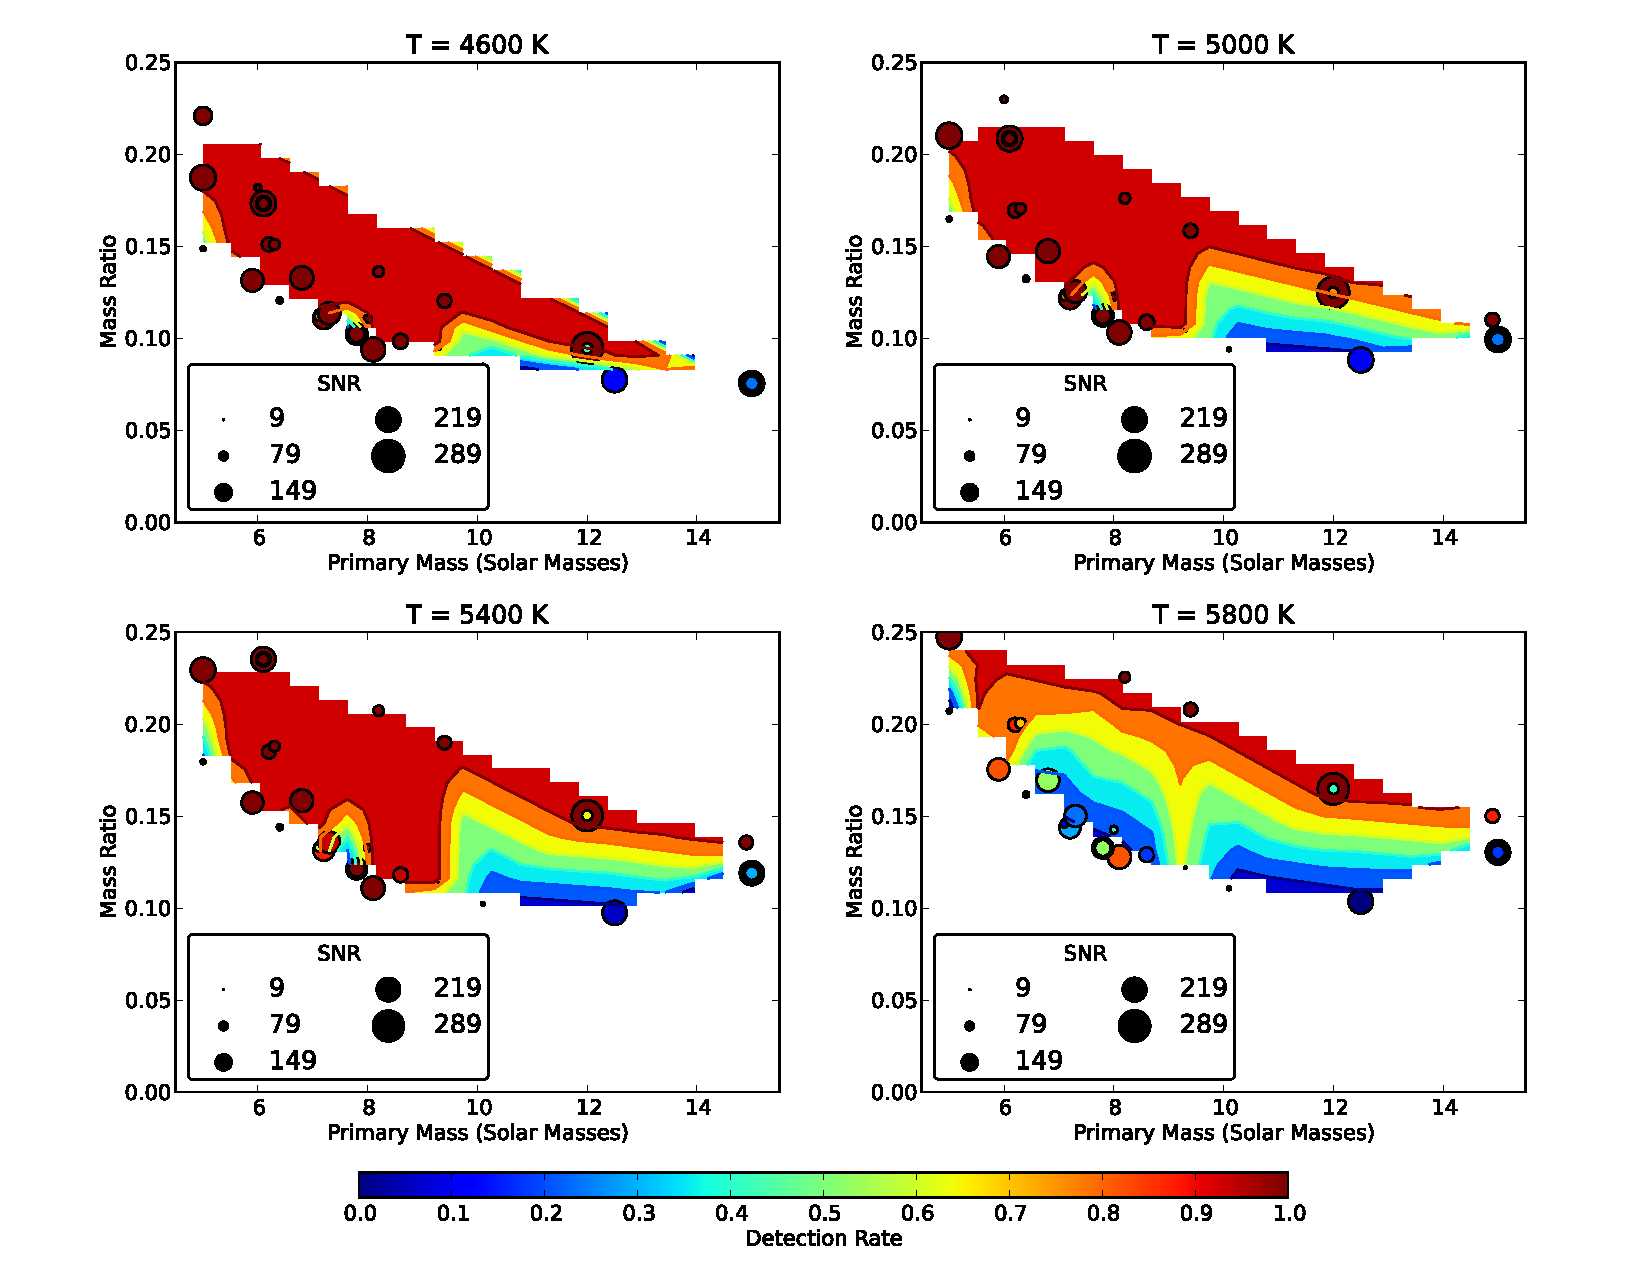
\includegraphics[width=5.5in]{Figures/paper1_fig6.pdf}
  \caption{Completeness diagram for the full sample of main-sequence B
  stars, split up by the effective temperature of the secondary
  star. The points correspond to the individual stars in the sample,
  and their sizes reflect the signal-to-noise ratio in the
  spectrum. Note that the signal-to-noise is calculated after the
  telluric line removal, and counts any telluric residuals as
  noise. The figures are also color-coded by the fraction of trials
  that detected the companion (see section
  \ref{paper1_sec:completeness}). Contours are drawn to guide the eye. The red 
  areas in each plot indicate the regions for which our sample is complete.}
  \label{paper1_fig:completeness}
\end{figure*}

If HIP 92855 is a true binary system, evolutionary tracks by
\cite{Landin2008} give a secondary star mass of $1.2 \pm 0.2 M_{\odot}$. The mass of the
primary star is $7.8 \pm 0.2 M_{\odot}$ \citep{Tetzlaff2010}, giving a mass
ratio of $q = 0.15 \pm 0.04$. The maximum radial velocity, observed on 2007 August 2, was 234 km s$^{-1}$. If this is the radial velocity semi-amplitude and if the companion is on a circular orbit, the binary orbit would have a period of 6.8 days. If the true velocity semi-amplitude is larger either because no observation was taken when the companion star was at quadrature or because the orbit is inclined, the period would be shorter than this. If the companion star is on an eccentric orbit, the period could be longer than 6.8 days if the large velocity observed was near periastron.




\section{Completeness}
\label{paper1_sec:completeness}
We now estimate the completeness of the direct spectral detection
method applied to this data set. For each telluric-corrected observation, we
created a series of synthetic binary-star spectra by adding stellar models to
the data at various flux ratios, temperatures, and radial
velocities. We used evolutionary tracks from \cite{Landin2008} to
find the luminosity of model companion stars with temperatures ranging from 3000K to
7000K in steps of 500 K. To find the model flux ratio $F_s/F_p$, we
used the best-fit age for each star quoted in
Table \ref{paper1_tab:sample}, as well as the best-fit age$\pm
\sigma_{age}$. Model secondary spectra generated with the Phoenix code
\citep{Hauschildt1999} were added to the telluric-corrected
observations at 17 different radial velocities ranging
from -400 to +400 km s$^{-1}$. Changing the radial velocity of the model
spectrum changes where the companion spectral lines fall with respect
to the telluric lines. Finally, we cross-correlated each synthetic
spectrum with its corresponding model secondary star spectrum, and examined the cross
correlation function. 

If the highest peak in the cross-correlation function was at the
correct velocity, the companion was considered detected. We then
tabulated how many times the companion star was detected in the 17
radial velocity trials. Figure \ref{paper1_fig:completeness} shows the
fraction of trials that detected the companion for all of the model
radial velocities, as a function of primary (B-star) mass and the binary mass-ratio. The points
correspond to individual spectra, with their sizes indicating the
signal-to-noise ratio in the spectrum, and the contours are drawn by
interpolating between the points.  The four panels are for different companion star temperatures. Companion stars with effective
temperatures from $4600-5400$ K have large regions with a very high
detection rate. Stars cooler than about 4600 K are too dim to detect
without much higher signal-to-noise ratios than present in our dataset, and stars hotter than about
5400 K do not have a strong CO bandhead and so the cross-correlation
function is not as sensitive. 

Figure \ref{paper1_fig:completeness} shows that the direct spectral detection
method is able to find companion stars with a mass-ratio of $q\approx
0.1-0.2$, for a range of effective temperatures. The regions with a 
detection rate near 1 are completely sampled, and a companion star in 
that region would be detected. For primary stars with $M < 10 M_{\odot}$, we are sensitive to almost all companions with $4600 < T_\mathrm{eff} < 5400$ K.




\begin{figure*}[ht]
  \centering
  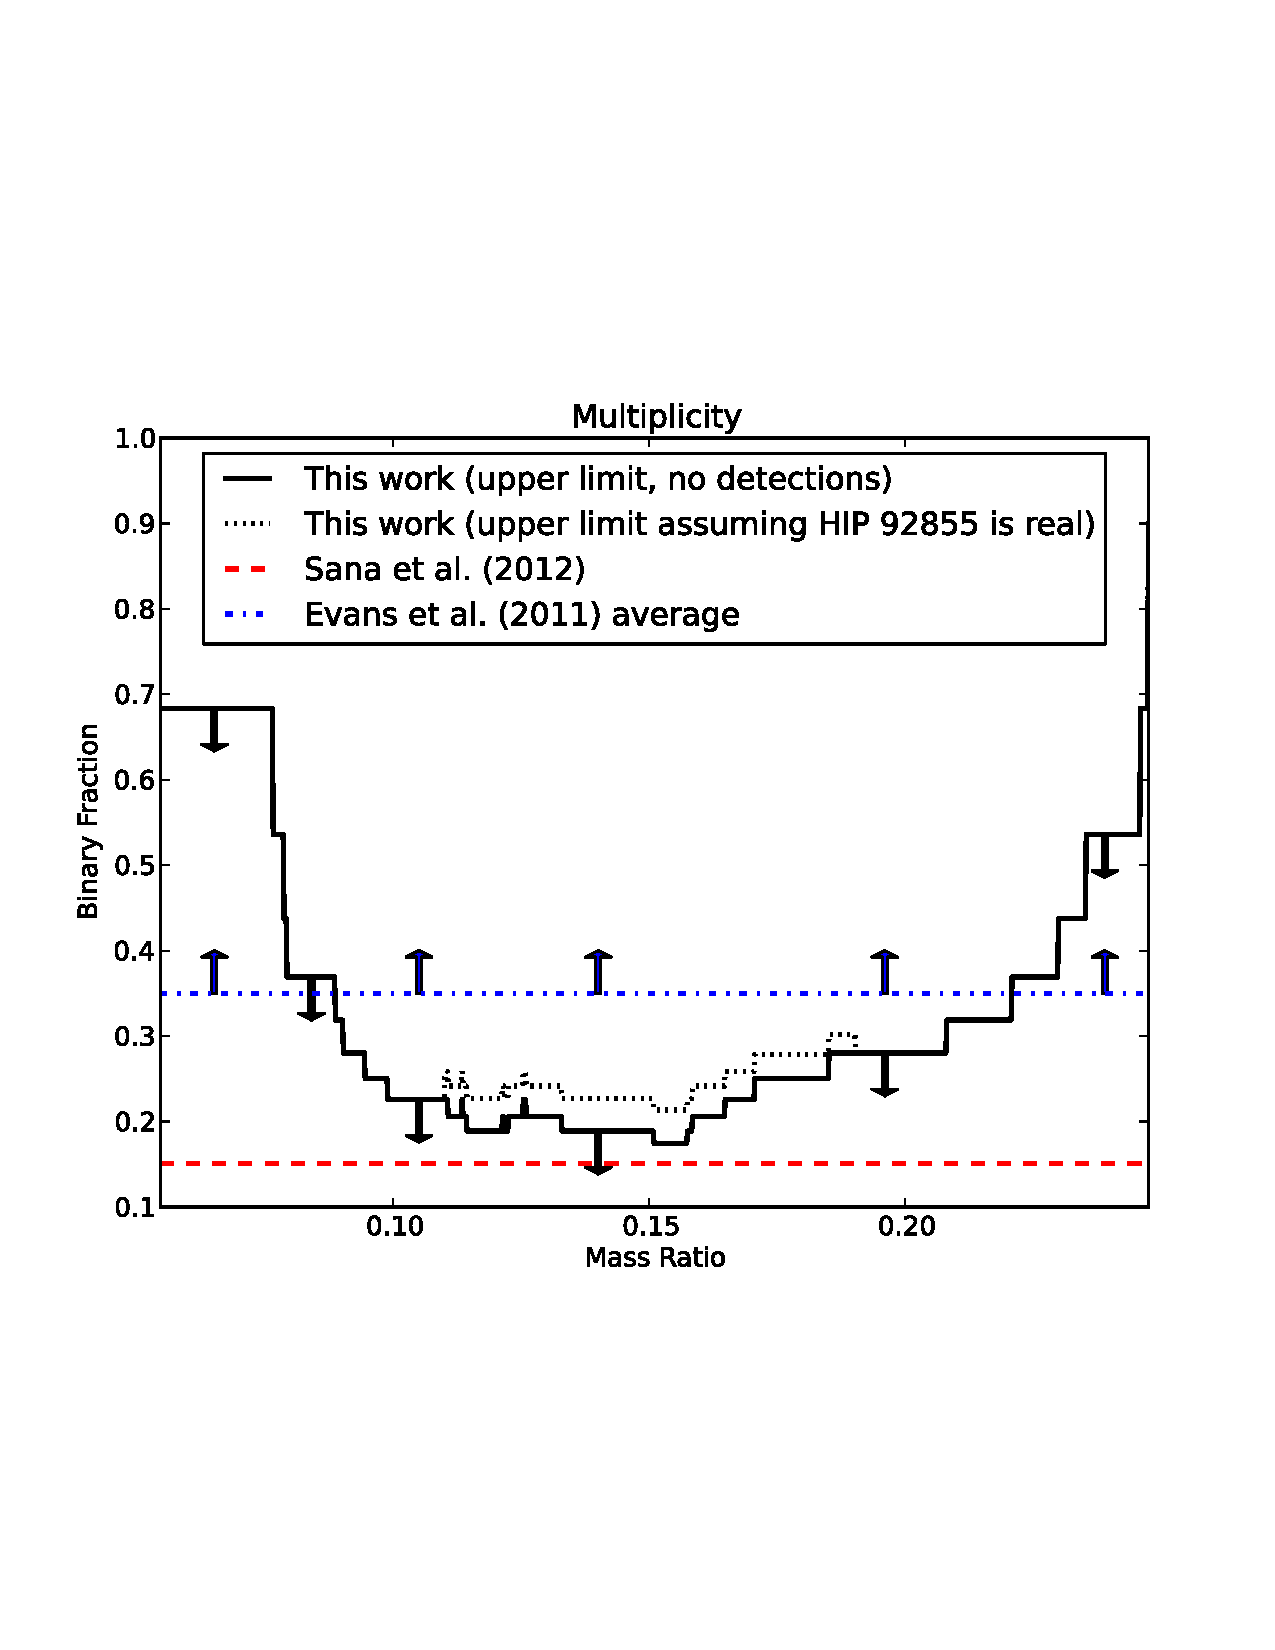
\includegraphics[width=\columnwidth]{Figures/paper1_fig7.pdf}
  \caption{Estimates of the binary fraction of B0-B5 stars,
    as a function of binary mass-ratio. This work found no unambiguous companions,
    and so we give $90\%$ upper limits (solid black line). $90\%$
    upper limits are also given assuming that HIP 92855 is a real
    binary system (dotted black line). The upper limits are only different within the
    $1\sigma$ error bars on the mass-ratio for HIP 92855. The nearly flat 
    distribution found by \cite{Sana2012} is shown as the dashed red line. The average binary 
    fraction found by \cite{Evans2011} is also shown (dash-dot blue line). The
    \cite{Evans2011} value is a \emph{lower} limit and an average over all mass-ratios from $0.1 < q < 0.3$, but they estimate
    that their sample is very complete, and so the true multiplicity fraction is quite close to their value.}
  \label{paper1_fig:limits}
\end{figure*}


\section{Multiplicity Fraction}
\label{paper1_sec:multiplicity}

We have not found any unambiguous low mass-ratio companions in our
sample, though we do have two candidates that require follow-up
observations (HIP 92855 amd HIP 26713). From the work described in section
\ref{paper1_sec:completeness}, we define a range
of mass-ratios for which the direct spectral detection method is
sensitive for each primary (B-) star. We can then rule out any
companions with mass-ratios in that range, for that primary star.

In order to convert these star-by-star limits on the presence of a
companion into upper limits on the multiplicity
fraction of the parent population, we first count the number of stars
that rule out companions in a particular range of mass-ratios. We then
apply binomial statistics, where the probability P of finding k
companions from n samples of a parent population with a true binary
fraction p is given by

\begin{equation}
P(k|p,n) = \frac{n!}{k!(n-k)!}p^k(1-p)^{n-k}
\label{paper1_eqn:binomial}
\end{equation}

For no detected binary companions (k=0), the corresponding likelihood
function for the binary fraction is

\begin{equation}
P(p|k=0, n) = (n+1)\cdot  (1-p)^n
\label{paper1_eqn:likelihood}
\end{equation}

A $90\%$ upper limit is given by

\begin{equation}
0.9 = \int_0^p (n+1)\cdot  (1-p')^n dp'
\label{paper1_eqn:limitdef}
\end{equation}

with solution

\begin{equation}
p_{90} = 1 - 0.1^{\frac{1}{n+1}}
\label{paper1_eqn:limit}
\end{equation}

A similar derivation gives $90\%$ upper limits for one detection (k=1).
Figure \ref{paper1_fig:limits} shows the $90\%$ upper limits to the binary
fraction as a function of mass-ratio. To find n in equation
\ref{paper1_eqn:limit}, we counted the number of stars that ruled out a
companion at the given mass-ratio. We only counted companions that
were found in all 17 radial velocity trials (see section
\ref{paper1_sec:completeness}), and were always found with at least $4\sigma$
significance. We also included upper limits assuming that HIP 92855, the more likely of our two candidates, is
a true binary system. Figure \ref{paper1_fig:limits} also shows the lower
multiplicity limit set by \cite{Evans2011} (blue dotted line) and the
\emph{intrinsic} O star mass-ratio distribution derived by
\cite{Sana2012}. \cite{Evans2011} do not split their multiplicity by mass-ratio,
and so the line shown in figure \ref{paper1_fig:limits} is an average value. While
we include them for comparison with our results, neither of these studies are
directly comparable to our sample. \cite{Sana2012} have only O stars in
their sample and are only able to measure mass-ratios $q\approx
0.2-1$, although they consider mass-ratios down to $q=0.1$
when deriving the intrinsic distribution. \cite{Evans2011} are sensitive to similar mass-ratios as our
sample, but they sample late B-stars (B4-B9) while we sample early B
stars (B0-B5). Our results are almost perfectly complementary to those of \cite{Evans2011}. It
is encouraging that our upper limits for $0.1<q<0.2$, where our sample
is most complete, lie in between the results of
\cite{Sana2012} who measure the binary fraction of more massive
primaries, and \cite{Evans2011} who measure the binary fraction of
less massive primaries than we do.

The above analysis assumes that the sample of B-stars given in Table
\ref{paper1_tab:sample} is representative of the B-star population as a
whole. Most of the sample stars are field
B-stars, which have a lower overall multiplicity than cluster or
association B-stars \citep{Mason2009}. However, the close binaries this
method is sensitive to would be difficult to disrupt with dynamical
interactions in a cluster environment, and we therefore expect this
sample to be representative of both populations. A potential complication is that telluric standard stars are often chosen specifically because they are \emph{not} known binary systems. While this may introduce a bias for large mass-ratios, the direct spectral detection method is sensitive to low mass-ratio companions that may not have been found with other methods such as classical spectroscopy or imaging and so companions with $q \lesssim 0.2$ may be less effected. The amount of bias introduced into the above measurement depends on how carefully the individual observers chose the telluric standard stars, and so is very difficult to assess.



\section{Conclusion}
\label{paper1_sec:conclusions}
We have described a new technique for finding binary systems with a
flux ratio of $F_p/F_s \approx 100$, where $F_p$ and $F_s$ are
the fluxes from the primary and secondary star, respectively. In this
technique, which we call the direct spectral detection technique, we
use high signal-to-noise, high resolution spectra of a binary candidate.
We remove the contamination from the Earth's atmosphere with the telluric 
modeling code LBLRTM, and cross-correlate the residuals with a library of stellar 
models for late type stars (F2-M5). A binary detection would appear as a strong 
peak in the cross-correlation function.

We prove the feasibility of the direct spectral detection method by
adding a synthetic signal to real data, and successfully recovering
it. We further investigate the completeness of the method in section \ref{paper1_sec:completeness}. This method is sensitive to detecting a range of companion stars, set by the spectral type and age of the primary and the signal-to-noise ratio of the observation. Our sample is sensitive to almost all companion stars with $4600 < T < 5400$, corresponding to binary mass-ratios of $0.1 \lesssim q \lesssim 0.2$.

 We have applied this technique to a sample of 34 archived main sequence 
early B-stars (B0-B5) with spectra taken with the CRIRES near-infrared
spectrograph. We found no unambiguous companions in our sample, but identify two targets as candidate binary systems: HIP 92855 and HIP 26713. HIP 92855 is B2.5V type star, with a candidate companion star with effective temperature $T = 6100$ K and mass $1.2 \pm 0.2 M_{\odot}$. Such a companion star is very near the detection limit of the direct spectral detection technique and deserves further follow-up observations. HIP 26713 is a B1.5V type star, with a candidate companion star with $T = 5600$ K and $M = 1.6 \pm 0.2 M_{\odot}$. This star was only observed once in our sample, and so may be a series of incompletely removed telluric absorption lines masquerading as a companion star.

We set upper limits on the binary fraction of early B stars as a function of binary mass-ratio (see Figure \ref{paper1_fig:limits}). As well as showing the upper limit for no detections in our sample, we also show the binary fraction upper limit assuming the HIP 92855 is a true binary system.  Our upper limits are strongest for mass-ratios $q \approx 0.1 - 0.15$, and are
about $20\%$. We compare our limits to the intrinsic binary mass-ratio distribution for O-type primaries derived by \cite{Sana2012}, as well as the lower limit \emph{average} binary fraction seen by \cite{Evans2011} for late B-stars (B4-B9). Our strongest upper limits ($0.1 \leq q \leq 0.15$) fall in between these two previous studies.

Companion stars formed by circumstellar disk instability are expected to have
typical mass-ratios near $q = 0.1$ \citep{Kratter2006,
  Stamatellos2011}, near where our upper limits are strongest. If there was
a large population of low mass-ratio companions formed by disk
fragmentation, we would expect to see a peak in the mass-ratio
distribution near $q \approx 0.1$. Since our results agree well with
the nearly flat mass-ratio distribution derived by \cite{Sana2012}, it
is unlikely that such a peak exists. There are several possible
interpretations of this result, three of which we give below.

\begin{enumerate}
\item Stellar companions formed by disk instability have a much lower
  characteristic mass-ratio than $q=0.1$ which remain invisible to
  observations.
\item The mass-ratio distribution of companions formed by disk
  instability is very broad, and so we would not expect a strong peak
  in the observed mass-ratio distribution. This interpretation may be
  supported by the flatness of the mass-ratio distribution as well as
  disk instability simulations that end with massive companions
  \citep[e.g.][]{Krumholz2009, Clarke2009}.
\item Disk instability is not a dominant formation mechanism for low
  mass-ratio binary systems, and molecular core fragmentation alone
  can generate the nearly flat mass-ratio distribution down to low mass-ratios.
\end{enumerate}

It is difficult to distinguish between these interpretations at this
time. More observational work, as well as computational work, is
required to explain the binary properties of high-mass stars. 

We would like to acknowledge Andreas Seifahrt, Rob Robinson, and Daniel Jaffe for their generous help with the telluric modeling 
procedure and some of the statistical aspects of this work. We would
also like to thank the referee for a quick review and many helpful comments. This 
research has made use of the 
following online resources: the SIMBAD database and the VizieR
catalogue access tool at CDS, Strasbourg, France, and the ESO Science 
Archive Facility. Funding for this work was provided by a National Science Foundation CAREER award to Sarah Dodson-Robinson (AST-1055910) and by start-up funding from the University of Texas College of Natural Sciences.


%%%%%%%%%%%%%%%%%%%%%%%%%%%%%%%%%%%%%%%%%%%%%%%%%%%%%%%%%
%%                Tables                           %%%%%%
%%%%%%%%%%%%%%%%%%%%%%%%%%%%%%%%%%%%%%%%%%%%%%%%%%%%%%%%%

%\begin{center}
\begin{small}
\begin{longtable}{|cccccc|}
    %\tablecaption{Full star sample}
    %\tablefirsthead{\hline Star & Spectral Type & Age (Myr) & Distance
      %(pc) & Maximum Separation (AU) \\ \hline} 

    %\tablehead{\multicolumn{5}{c}{{\tablename} \thetable{} -- Continued} \\ \hline Star &
     % Spectral Type & Age (Myr) & Distance (pc) & Maximum Separation (AU) \\ \hline} 

    %\tabletail{\hline}

   % \tablelasttail{\hline}

    \caption{Full star sample} \\
        \hline
       & & & & Maximum & Number of \\ Star & Spectral Type & Age (Myr) & Distance
       (pc) & Separation (AU) & Observations \\ \hline
        \endfirsthead

        \multicolumn{6}{c}{{\tablename} \thetable{} -- Continued} \\
        \hline
         & & & & Maximum & Number of \\ Star & Spectral Type & Age (Myr) & Distance
       (pc) & Separation (AU) & Observations \\ \hline
        \endhead

        \hline
        \endfoot

        \hline
        \endlastfoot

%    \begin{supertabular}{| c c c c c |}
%        HIP 108975 & B3V (+B)  &$ 50.1 \pm 10.9 $& 19.96 & 15.97 & 2 \\ 
        HIP 23364 & B3V &$ 31.6 \pm 0.6 $& 31.65 & 25.32 & 1 \\ 
        HIP 26713 & B1.5V &$ 7.2 \pm 2.5 $& 138.89 & 111.11 & 1 \\ 
        HIP 27204 & B1IV/V & $12.6 \pm 4.6$ & 408.2 & 326.5 & 1 \\
    HIP 30122 & B2.5V & $32 \pm 0.4$ & 111.1 & 88.9 & 4 \\
    HIP 32292 & B2V & $8.2 \pm 0.1$ & 1111.1 & 888.9 & 1 \\
    HIP 39866 & B3V & $25.1 \pm 2.6$ & 840.3 & 672.3 & 1 \\
    HIP 48782 & B3V & $32.3 \pm 0.6$ & 370.4 & 296.3 & 1 \\
        HIP 52370 & B3V &$ 17.2 \pm 1.3 $& 58.14 & 46.51 & 2 \\ 
        HIP 52419 & B0Vp &$ 4 \pm 0.7 $& 250 & 200 & 2 \\ 
    HIP 54327 & B2V & $11.7 \pm 6.2$ & 252.5 & 202.0 & 3 \\
    HIP 55667 & B2IV-V & $22.5 \pm 2.6$ & 847.5 & 678.0 & 1 \\
        HIP 60823 & B3V &$ 25.3 \pm 6.3 $& 39.53 & 31.62 & 5 \\ 
        HIP 62327 & B3V &$ 8.2 \pm 1.8 $& 121.95 & 97.56 & 4 \\
        HIP 63945 & B5V &$ 27.3 \pm 11.4 $& 36.63 & 29.3 & 1 \\  
    HIP 61585 & B2IV-V & $18.3 \pm 3.2$ & 96.7 & 77.4 & 8 \\
    HIP 62327 & B3V & $8.2 \pm 1.8$ & 117.9 & 94.3 & 4 \\
    HIP 63007 & B4Vne & $53.3 \pm 8.1$ & 117.6 & 94.1 & 2 \\
    HIP 63945 & B5V & $27.3 \pm 11.4$ & 119.6 & 95.7 & 1 \\
    HIP 67796 & B2V & $15.4 \pm 0.4$ & 970.9 & 776.7 & 1 \\
        HIP 68282 & B2IV-V &$ 13 \pm 2 $& 76.92 & 61.54 & 2\\ 
        HIP 68862 & B2V &$ 9.1 \pm 3.8 $& 109.89 & 87.91 & 1 \\ 
        HIP 71352 & B1Vn + A &$ 5.6 \pm 1 $& 178.57 & 142.86 & 2 \\ 
        HIP 73129 & B4Vnpe &$ 27.1 \pm 6.1 $& 36.9 & 29.52 & 1 \\ 
        HIP 74110 & B3V &$ 33.2 \pm 7.3 $& 30.12 & 24.1 & 1 \\ 
        HIP 76126 & B3V &$ 15.9 \pm 1.3 $& 62.89 & 50.31 & 1 \\ 
        HIP 78820 & B0.5V & $13.8 \pm 0.4$ & 123.9 & 99.1 & 1 \\
        HIP 80582 & B4V &$ 50.1 \pm 14 $& 19.96 & 15.97 & 2 \\ 
        HIP 80815 & B3V &$ 10.5 \pm 2.1 $& 95.24 & 76.19 & 4 \\ 
        HIP 81266 & B0.2V &$ 5.7 \pm 1 $& 175.44 & 140.35 & 12 \\ 
        HIP 82514 & B1.5Vp+ &$ 20 \pm 2 $& 50 & 40 & 1 \\ 
        HIP 87314 & B2/B3Vnn &$ 23.2 \pm 2.9 $& 43.1 & 34.48 & 7 \\ 
        HIP 92855 & B2.5V &$ 31.4 \pm 0.4 $& 31.85 & 25.48 & 7 \\ 
        HIP 92989 & B3V &$ 7.9 \pm 2.1 $& 126.58 & 101.27 & 1 \\ 
%        HIP 94385 & B3V &$ 27.9 \pm 4.1 $& 35.84 & 28.67 & 2 \\
        HIP 97611 & B5V &$ 45 \pm 10 $& 66.67 & 53.33 & 1        
 %       \tablecomments{The maximum
%separation column estimates the approximate separation of the binary
%orbit we are sensitive to, assuming a seeing of 0.8''}
%      \end{supertabular}

        \label{paper1_tab:sample}
\end{longtable}
\end{small}
%\end{center}

\newpage
%\begin{center}
   \begin{longtable}{|cccc|}
      \caption{Summary of adjusted line strengths. The units of line
        strength are cm$^{-1}$/(molecule $\times$ cm$^{-2}$)} \\
        \hline
        Wavelength (nm) & Molecule & Old Strength & New Strength \\ \hline \hline
        \endfirsthead

        \multicolumn{4}{c}{{\tablename} \thetable{} -- Continued} \\
        \hline
        Wavelength & Molecule & Old Strength & New Strength \\ \hline \hline
        \endhead

        \hline
        \endfoot

        \hline
        \endlastfoot

        2317.12   &   CH$_4$   &   5.445\e{-21}   &   5.034\e{-21} \\
        2318.24   &   H$_2$O   &   1.400\e{-24}   &   2.256\e{-24} \\
        2328.51   &   CH$_4$   &   2.521\e{-21}   &   2.371\e{-21} \\
        2328.56   &   CH$_4$   &   1.270\e{-21}   &   1.358\e{-21} \\
        2340.12   &   CH$_4$   &   3.085\e{-21}   &   2.963\e{-21} \\
        2340.36   &   CH$_4$   &   3.343\e{-21}   &   3.211\e{-21} \\
        2351.64   &   H$_2$O   &   1.670\e{-23}   &   1.393\e{-23} \\
        2351.69   &   H$_2$O   &   1.085\e{-23}   &   7.985\e{-24} \\
        2352.43   &   CH$_4$   &   3.144\e{-23}   &   4.031\e{-24} \\
        2352.45   &   H$_2$O   &   4.639\e{-23}   &   4.939\e{-23} \\
        2353.62   &   CH$_4$   &   2.708\e{-21}   &   2.654\e{-21} \\
        2355.82   &   CH$_4$   &   5.101\e{-21}   &   4.949\e{-21} \\
        2358.9     &   CH$_4$   &   5.160\e{-21}   &   4.710\e{-21} \\
        2364.03   &   H$_2$O   &   1.408\e{-23}   &   1.217\e{-23} \\
        2367.23   &   H$_2$O   &   2.078\e{-23}   &   2.182\e{-23} \\
        2370.35   &   CH$_4$   &   4.028\e{-21}   &   3.625\e{-21} \\
        2370.41   &   CH$_4$   &   2.437\e{-21}   &   2.021\e{-21} \\
        2370.75   &   CH$_4$   &   1.466\e{-21}   &   9.138\e{-22} \\
        2371.39   &   H$_2$O   &   3.905\e{-23}   &   3.171\e{-23} \\
        236.62     &   H$_2$O   &   1.146\e{-23}   &   9.186\e{-24} \\
        2376.63   &   H$_2$O   &   3.824\e{-24}   &   3.820\e{-24} \\
        2378.2     &   H$_2$O   &   1.134\e{-22}   &   1.021\e{-22} \\
        2379.67   &   H$_2$O   &   6.334\e{-24}   &   8.408\e{-24} \\
        2385.98   &   H$_2$O   &   6.051\e{-23}   &   5.407\e{-23}
        
        
    \label{paper1_tab:linelist}
  \end{longtable}
%\end{center}
  
  
  
%\begin{center}
 \begin{small}
   \begin{longtable}{|ccp{6cm}|}
      \caption{Summary of Cross-Correlation Function Peak Rejection Steps. See Section \ref{paper1_sec:results} for more information} \\
        \hline
        Step  & Description & Method \\ \hline
        \endfirsthead

        \multicolumn{3}{c}{{\tablename} \thetable{} -- Continued} \\
        \hline
        Step  & Description & Method \\ \hline
        \endhead

        \hline
        \endfoot

        \hline
        \endlastfoot

        1 & Telluric Residual Peak Identification & Compare cross-correlation function of telluric-corrected spectrum with that of an uncorrected spectrum. \\

        \hline
        2 & Sensitivity Analysis & Check that signal-to-noise ratio
        is high enough to detect secondary candidate at a range of velocities \\

        \hline
        3 & Velocity Analysis & Check that a blackbody with the
        candidate temperature can exist as close to the primary B-star as the velocity indicates (assumes circular orbit)
        
        
    \label{paper1_tab:rejection}
  \end{longtable}
 \end{small}
%\end{center}

\scriptsize 
\begin{samepage}
%\begin{center}
\begin{longtable}[t]{|lcccc|}

\caption{Summary of HIP 92855 observations. Significance is in units of
  the standard deviation of the cross-correlation function. The detection rate and expected significances are from the sensitivity analysis (Table \ref{paper1_tab:rejection}, step 2).} \\
\hline
Date & Detection Rate & Expected Significance & Observed Significance
& Velocity (km s$^{-1}$) \\ \hline
\endfirsthead

\multicolumn{4}{c}{{\tablename} \thetable{} -- Continued} \\
\hline
Date & Detection Rate & Expected Significance & Observed Significance
& Velocity (km s$^{-1}$) \\ \hline
\endhead

\hline
\endfoot

\hline
\endlastfoot

2007 May 9 & 0.35 & 3.3 $\sigma$ & 4.1 $\sigma$ & -74 \\
2007 June 9 & 0.18 & 3.6 $\sigma$ & N/A & N/A \\
2007 July 25 & 0.35 & 3.7 $\sigma$ & N/A & N/A \\
2007 August 2 & 0.47 & 3.6 $\sigma$ & 3.5 $\sigma$ & -234 \\
2007 September 16 & 0.82 & 4.2 $\sigma$ & N/A & N/A \\
2008 September 19 & 0.71 & 3.4 $\sigma$ & 4.1 $\sigma$ & -126 \\
2008 September 10 & 0.59 & 3.3 $\sigma$ & 4.0 $\sigma$ & 116 
\label{paper1_tab:hip92855}
\end{longtable}
%\end{center}  
\end{samepage}
%Return to normal font size
\normalsize

%%%%%%%%%%%%%%%%%%%%%%%%%%%%%%%%%%%%%%%%%%%%%%%%%%
% Chapter 6  (main survey)
%%%%%%%%%%%%%%%%%%%%%%%%%%%%%%%%%%%%%%%%%%%%%%%%%%


\chapter{The Inner Mass-Ratio Distribution of Intermediate-Mass Stars}
\label{chap:survey}

Finally, we use the direct spectral detection method to perform a large survey aimed at detected cool companions to hot A- and B-type stars. This chapter has been submitted for publication to the Astronomical Journal.



\section{Introduction}
\label{paper6_sec:intro}

Stellar multiplicity is an inevitable and common outcome of star formation, with roughly half of all solar-type field stars in binary or multiple systems \citep{Raghavan2010} and an even higher fraction as the stellar mass increases \citep{Zinnecker2007}. Young stellar associations and clusters tend to have even higher multiplicity \citep{Duchene2013}, indicating that stars often form in multiple systems that are subsequently destroyed by dynamical interactions as the cluster dissociates. 

The overall multiplicity rate and the distributions of mass ratio, period, and eccentricity of a binary star population place important constraints on the mode of binary star formation. While the period and eccentricity are altered by dynamical processing in the birth cluster, the present-day mass ratio of a binary system is a direct result of its formation \citep{Parker2013}. Most binary stars are thought to form via core fragmentation \citep{Boss1979, Boss1986, Bate1995}, in which a collapsing core fragments into two or more individual protostars. The number and initial masses of the fragments are set by the total core mass, as well as its rotation, turbulence, and its temperature and density structure. If the fragments are well separated ($a \gtrsim 1000$ AU), they will evolve independently of each other, accreting mass from the core material onto their own protostellar disks and then onto the protostars themselves. However close fragments ($a \sim 100$ AU) will interact with each other; the protostellar disk may be truncated, destabilized, or form into a circumbinary disk if the separation is small enough \citep{Bate1997}. In addition, an unstable disk can fragment to form low-mass companions \citep{Kratter2006, Stamatellos2011}. The mass ratios of close companions formed via either mechanism should be affected by preferential accretion. Most work has suggested that the disk material will preferentially accrete onto the lower mass companion \citep{Bate1997, BBB2002}; however, recent work has indicated that magnetic disk braking may result in preferential accretion onto the more massive component \citep{Zhao2013} instead. In either case, we would expect to find a mass-ratio distribution for companions inside a few $100$ AU that differs from that of companions on wider orbits.

The mass ratio, period, and eccentricity distributions are fairly well-known for solar type stars \citep{Duquennoy1991, Raghavan2010} and cooler stars \citep{Fischer1992, Delfosse2004}. Interestingly, the mass-ratio distribution appears to be invariant to separation for these stars \citep{Meyer2013}, contrary to the theoretical expectations. All of the distributions are much less certain for more massive stars. The reason for this is two-fold: first, more massive stars tend to more rare and farther away, meaning many of the companions are angularly close to the very bright primaries and difficult to detect with imaging techniques. Second, the primary stars tend to be rapid rotators, which limits radial velocity precision to $\sim 1 \mathrm{km\ s}^{-1}$. Additionally, radial velocity monitoring can only measure a mass ratio if spectral lines from both components are visible; this typically suffers from the same flux ratio difficulty as imaging techniques. 

Nonetheless, \citet{DeRosa2014} performed an adaptive optics imaging survey of nearby A-type stars, and found that the mass-ratio distribution is well-described by a power law with large slope, indicating a very strong preference for low-mass companions. They also found initial evidence that the mass-ratio distribution for companions inside $125$ AU has a much shallower power law slope than that of wide companions, and is consistent with flat. Their close companion subsample contained only 18 binary systems, and the result is complicated by the inherent difficulty of detecting close companions with low mass ratios in an imaging survey. 

Radial velocity monitoring surveys can detect much closer companions than imaging surveys, but are typically only complete to low-mass companions if the primary is a slow rotator. Chemically peculiar Am stars are typically associated with binary companions, and are slow rotators due to tidal braking; they thus form a highly biased sample of intermediate-mass stars. Nonetheless, it is interesting to note that they have a mass-ratio distribution which peaks near $q \sim 0.5$ \citep{Vuissoz2004}, an entirely different form than the distribution found around chemically normal stars at wide separations.

In this paper, we describe a spectroscopic survey of nearby chemically normal, main sequence intermediate-mass stars ($M \approx 1.5 - 15 M_{\odot}$). We search for companions using the direct spectral detection technique \citep{Gullikson2016}, which has a separation-invariant detection rate for all separations inside $\sim 1 ''$. We describe the stellar sample and data used for the survey in Section \ref{paper6_sec:obs}, as well as the data reduction steps in the same section. Next, we describe the direct spectral detection method and tabulate the companion detections in Section \ref{paper6_sec:companions}. We estimate the mass and age of the sample stars in Section \ref{paper6_sec:sp}, and discuss the survey completeness in Section \ref{paper6_sec:completeness}. Finally, we end with a derivation of the mass-ratio distribution from our sample in Section \ref{paper6_sec:mrd} and discuss its implications for binary formation in Section \ref{paper6_sec:discussion}.
 


\section{Observations and Data Reduction}
\label{paper6_sec:obs}

The stellar sample for this survey is defined by the following criteria:

\begin{itemize}
\item $V < 6$ mag
\item $v\sin{i} > 80 \mathrm{km\ s}^{-1}$
\item Spectral Type A or B with the following additional constraints
\begin{itemize}
  \item Main Sequence
  \item No spectral peculiarities except for `n', which denotes broad lines.
\end{itemize}
\end{itemize}

The magnitude limit ensures that a sufficiently high signal-to-noise ratio can be achieved in a short period of time. It does introduce a Malmquist bias in the derived mass ratio, which we discuss and correct for in Section \ref{paper6_sec:mrd}. Likewise, the $v\sin{i}$ limit makes accounting for the primary star spectrum in the companion search trivial; since most A- or B-type stars are rapid rotators, the cutoff removes less than half of the stars from the potential sample. We exclude pre-main sequence stars because both the primary and the companion mass would depend very strongly on young and uncertain ($\lesssim 1$ Myr) evolutionary models. Finally, we exclude post-main sequence stars from our sample because the binary flux ratio would be even less favorable to companion detection in an evolved star. Most of the spectral peculiarities denote narrow lines, which are already removed from the sample by the $v\sin{i}$ cut. The sample is given in Table \ref{paper6_tab:sample}. The spectral type, coordinates, V magnitude, and parallax are all adopted from the Simbad Database \citep{Simbad}, while the stellar effective tempreature, surface gravity, masses, and ages are discussed in Section \ref{paper6_sec:sp}.

\subsection{Spectroscopic Data}
\label{paper6_subsec:specdata}
We use several high spectral resolution, cross-dispersed \'echelle spectrographs for this survey. We use the CHIRON spectrograph \citep{CHIRON} on the 1.5m telescope at Cerro Tololo Inter-American Observatory for most southern targets. This spectrograph is an $R\equiv \lambda / \Delta \lambda = 80000$ spectrograph with wavelength coverage from 450 - 850 nm, and is fed by a $2.7''$ optical fiber. The data are automatically reduced with a standard CHIRON data reduction pipeline, but the pipeline leaves residuals of strong lines in adjacent orders. We therefore bias-correct, flat-field and extract the spectra with the optimum extraction technique \citep{Horne1986} using standard IRAF\footnote{IRAF is distributed by the National Optical Astronomy Observatories, which are operated by the Association of Universities for Research in Astronomy, Inc., under cooperative agreement with the National Science Foundation.} tasks, and use the wavelength calibration from the pipeline reduced spectra.

For the northern targets, we use a combination of the High Resolution Spectrograph \citep[HRS,][]{HRS} on the Hobby Eberly Telescope, and the Tull coud\'e \citep[TS23,][]{TS23} and IGRINS \citep{IGRINS} spectrographs, both on the 2.7m Harlan J. Smith Telescope. All three northern instruments are at McDonald Observatory. For the HRS, we use the $R = 60000$ setting with a $2''$ fiber, and with wavelength coverage from 410-780 nm. We bias-correct, flat-field, and extract the spectra using an IRAF pipeline very similar to the one we use for the CHIRON data. The HRS spectra are wavelength-calibrated using a Th-Ar lamp observed immediately before or after the science observations.

For the TS23 spectrograph, we use a $1.2''$ slit in combination with the E2 \'echelle grating (53 grooves/mm, blaze angle $65^{\circ}$), yielding a resolving power of $R=60000$ and a wavelength coverage from 375-1020 nm. We reduce the data using an IRAF pipeline very similar to the ones we use for CHIRON and HRS, and wavelength calibrate using a Th-Ar lamp observed immediately before the science observations.

IGRINS has a single setting with $R = 40000$. It has complete wavelength coverage from $1475-2480$ nm, except in the telluric water band from $1810 - 1930$ nm. Each star is observed in an ABBA nodding mode, and reduced using the standard IGRINS pipeline \citep{IGRINS_plp_v2}. The standard pipeline uses atmospheric OH emission lines as well as a Th-Ar calibration frame to calibrate the wavelengths; we further refine the wavelength solution using telluric absorption lines in the science spectrum.

After reducing the data, we fit and remove the telluric spectrum using the TelFit code \citep{Gullikson2014}. We fit each \'echelle order affected by telluric absorption independently from each other to get the best removal. The telluric correction is critical for IGRINS spectra, where every order is dominated by telluric absorption lines. For the optical spectra, it is less critical but allows us to use some of the redder orders than we otherwise would be able to. For unsaturated lines, the best-fit telluric model reproduces the data to within $\sim 1-5\%$ of the continuum level.

We give the spectroscopic observation log in Table \ref{paper6_tab:observations}. We calculate the signal-to-noise ratio (the ``snr'' column) for the optical instruments (CHIRON, TS23, and HRS) as the median of the extracted flux divided by it's uncertainty for each pixel from the \'echelle order nearest $675$ nm. For the IGRINS instrument, we calculate the signal-to-noise ratio from the order nearest $2200$ nm.


\subsection{Imaging Data}
As part of the follow-up effort, we used the NIRI instrument behind the Altair adaptive optics system on the Gemini North Telescope. For each star listed in Table \ref{paper6_tab:imaging_obs}, we obtained 25 images in 5 dithering positions. We used the K-continuum band centered on $2.2718\ \mu m$ and a variety of exposure times and dates (listed in Table \ref{paper6_tab:imaging_obs}). Because the targets are all extremely bright, we used the high read noise and high flux detector settings to allow for very short co-add exposure times. We reduced the data using the Gemini set of IRAF tasks, which include steps for nonlinearity correction, flat-fielding, sky subtraction, and co-addition of the dither frames. 

We measure the flux and position of both stars by fitting a 2D Moffat function \citep{Moffat1969} to both stars simultaneously, constraining the shape parameters for both functions to be the same. The ratio of the amplitudes gives the magnitude difference, and the pixel locations along with the detector pixel scale gives the separation and position angle between the stars. We note that the goal of these images was confirmation and we did not observe any reference targets to make a distortion map and correct the image rotation. The uncertainty in position angle and to a lesser degree separation quoted in Table \ref{paper6_tab:imaging_obs} is likely underestimated.


\begin{figure*}
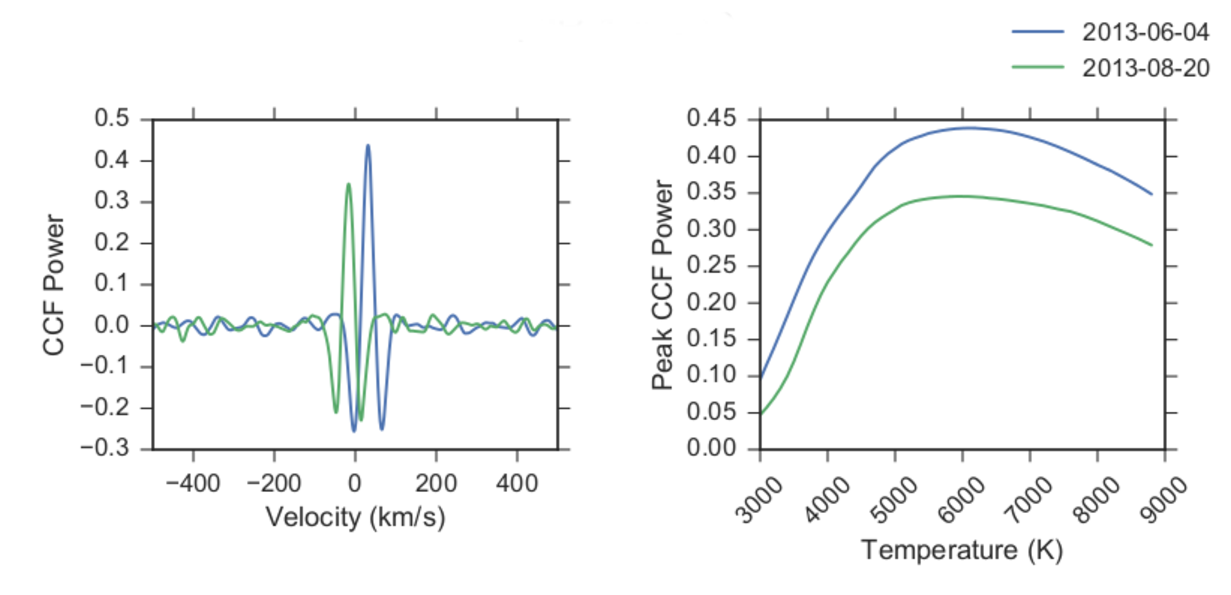
\includegraphics[width=\textwidth]{Figures/paper6_HIP_109139.pdf}
\caption{\emph{Left}: Cross-correlation function between the observed spectra of HIP 109139 and a $5700\ K$ Phoenix model spectra. The detection at two dates shows significant velocity variation, indicating orbital motion with a short period. \emph{Right}: Peak CCF height as a function of Phoenix model spectra template temperature. The maxima of the curves indicate the temperature of the companion.}
\label{paper6_fig:ccf}
\end{figure*}



\section{Companion Search}
\label{paper6_sec:companions}

We search for stellar companions to our sample stars using the direct spectral detection technique, described in detail in \citet{Gullikson2016}. In short, we unsharp-mask each spectrum using a gaussian filter with width proportional to the primary star $v\sin{i}$ to remove the broad lines from the primary star. We then cross-correlate each \'echelle order of each filtered spectrum against a large grid of Phoenix model spectra \citep{Husser2013_b} with the following parameters:

\begin{itemize}
\item $T_\mathrm{eff} = 3000-12000$ K, in steps of 100 K
\item {[}Fe/H{]} = -0.5, 0.0, +0.5
\item $v\sin{i} = 1, 5, 10, 20, 30 \ \mathrm{km\ s}^{-1}$
\end{itemize}

In order to be sensitive to hot companions, we additionally cross-correlate the spectra against a second grid of Kurucz model spectra \citep{Castelli2003}. The change in model is necessary because the Phoenix model library does not extend beyond $12000\ K$. The Kurucz grid is defined as follows:

\begin{itemize}
\item $T_\mathrm{eff} = 9000-30000$ K, in steps of 1000 K
\item {[}Fe/H{]} = -0.5, 0.0, +0.5
\item $v\sin{i} = 1, 5, 10, 20, 30, 40, 50 \ \mathrm{km\ s}^{-1}$
\end{itemize}

We combine the cross-correlation functions for all orders using both a simple average and the maximum-likelihood weighting scheme \citep{Zucker2003}. A companion detection is denoted by a strong peak in the combined cross-correlation function (CCF). While the maximum-likelihood scheme produces detections with much higher significance, it also magnifies spurious peaks and so has a larger false-positive rate. For this reason, we use the simple average CCFs in all further analysis.

The peak height in the CCF as a function of the stellar model acts in a similar way to the more typical $\chi^2$ map of parameter space. More concretely, as the stellar model template gets closer to the true companion spectrum, the CCF peak gets higher. We can therefore measure the companion temperature and, to a lesser degree its metallicity and $v\sin{i}$, in a single spectrum. Imperfect stellar models cause a bias between the true companion temperature and the temperature of the Phoenix model which produces the largest CCF peak. This bias is most pronounced at low temperatures, where the difficult-to-model molecular absorption becomes important. We correct for the bias by applying the calibrations developed in \citet{Gullikson2016}. These calibrations are only valid for companions with $3000 < T_\mathrm{eff} < 7000 K$; for detections at hotter temperatures we assume that the temperature which produces the maximum CCF peak is an \emph{unbiased} estimator of the true companion temperature.

We list the companion detections in Table \ref{paper6_tab:companions}, and report the estimate of the companion temperature, $v\sin{i}$, and metallicity derived from the model parameters which produce the largest CCF peak. The $v\sin{i}$ and metallicity values do not have uncertainties and should only be taken as a rough estimate of the true value. The mean and standard deviation of the companion metallicities is $-0.29 \pm 0.30$; the marginal bias towards low metallicities is most likely a measurement bias and does not reflect the true companion population \citep{Gullikson2016}.  We show the detection CCFs and a plot of peak CCF height as a function of model temperature for HIP 109139 in Figure \ref{paper6_fig:ccf}. Similar figures for all companions are available in the supplementary files.


We have follow-up spectroscopy for 15/23 of the new companions to confirm their existence. In most cases, there is a clear shift in the radial velocity of the companion, indicating that it is orbiting the target star and is not a foreground or background contaminant (See Figure \ref{paper6_fig:ccf}). Two of the new detections (companions to HIPs 38593 and 79404) were detected twice but not in a third attempt, most likely because the third spectrum had low signal-to-noise. The companion to HIP 93805, at $\sim 4000$ K, was detected twice with near-infrared IGRINS but not the optical CHIRON instrument that is less sensitive to cool companions than IGRINS. Two of the companions with only one detection were observed at least twice (HIPs 19949 and HIP 23362); both of the non-detections are from the IGRINS instrument, which is less sensitive to hot companions with rapid rotation speeds because there are far fewer spectral lines of the companion in the near-infrared than there are in the optical.


In addition to the spectroscopic follow-up, we obtained Gemini/NIRI adaptive optics imaging data for 18 of the northern companions, and were able to resolve 7 of them. We show the separation, position angle, and magnitude difference measurements in Table \ref{paper6_tab:imaging_obs}, and display the images in Figure \ref{paper6_fig:images}. We also derive the projected separation in AU and the companion mass from the images. We calculate the separation from the measured angular separation and the Hipparchos parallax \citep{Hipparchos}. We calculate the companion mass and uncertainties from 1000 samples of the magnitude difference measurement and the primary star mass, temperature, age, and radius (see Section \ref{paper6_sec:sp}). For each sample, we use a grid of Kurucz stellar model spectra \citep{Castelli2003}and the pysynphot code\footnote{pysynphot is a python package to perform synthetic photometry, and is available at this url: \url{https://pypi.python.org/pypi/pysynphot}} to determine the companion temperature needed to replicate the observed magnitude difference. We estimate the companion radius by interpolating solar metallicity Dartmouth isochrones \citep{Dotter2008} from the companion temperature and system age sample. We convert the best temperature to a companion mass using the same isochrone grid. The masses derived from the imaging data have very large uncertainties because the primary star property estimates that they depend on are very uncertain. The imaging masses agree with the spectroscopically-derived masses in Table \ref{paper6_tab:companions}, with the exception of HIP 115115 which has a much higher mass from the imaging data than the spectroscopic data. The spectroscopic masses for all stars are more reliable, since they are less model-dependent.

One star in the imaging sample, HIP 88116, has several nearby sources in the image. We quote the magnitude difference and separation of the brightest source in Table \ref{paper6_tab:imaging_obs}, but stress that \emph{none} of the visible sources is likely to be the companion we see in the spectroscopic data. The two epochs of spectroscopic data show a radial velocity shift of $\Delta v = 30.7\ \mathrm{km\ s}^{-1}$ over the course of roughly one year; this orbital motion is much too large to allow for any of the companions visible in the image (all with separations $ > 1''$ and projected separations $ > 300$ AU).

\begin{figure}
\centering
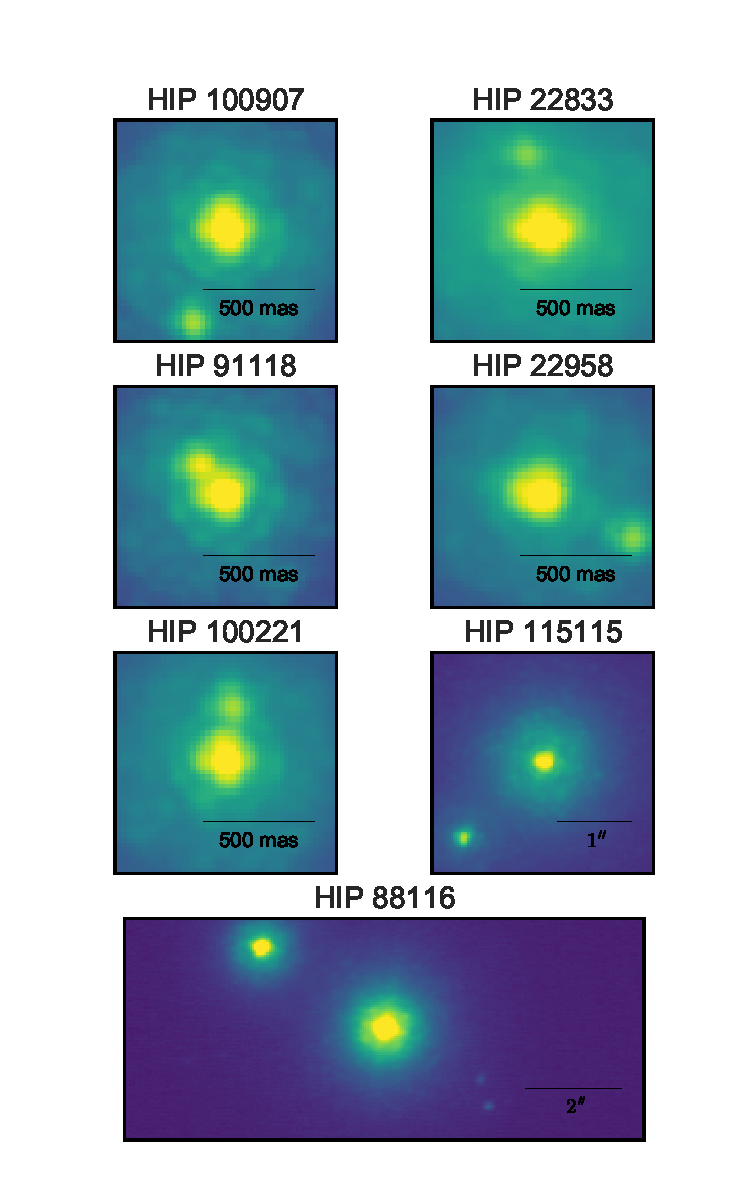
\includegraphics[width=4in]{Figures/paper6_Imaging_Data.pdf}
\caption{Detection images for all stars in which we detect a companion in the follow-up NIRI data. 
There are several nearby sources for HIP 88116, none of which are the source we detect in the 
spectroscopic data (see Section \ref{paper6_sec:companions}).}
\label{paper6_fig:images}
\end{figure}





\section{Sample Star Parameters}
\label{paper6_sec:sp}

In order to convert from companion temperature to mass ratio, we first need an estimate of the primary mass. In addition, since the primary stars in our survey have short main-sequence lifetimes, some companions may still be contracting onto the main sequence and so an age estimate for the system is necessary to convert from companion temperature to mass.

About half of our sample stars have robust mass and age estimates from Str\"omgren uvby$\beta$ photometry \citep{David2015}. For those that do not, we estimate the mass and age of the system from our spectra. We first cross-correlate the data against a grid of solar metallicity Kurucz model spectra \citep{Castelli2003} spanning

\begin{itemize}
\item $7000\ K < T_\mathrm{eff} < 30000\ K$ in steps of $1000\ K$
\item $3.0 < \log{g} < 4.5$ in steps of $0.5$ dex
\item $75 < v\sin{i} < 300\ \mathrm{km s}^{-1}$ in steps of $25\ \mathrm{km s}^{-1}$
\end{itemize}


For the optical data, we use the blue \'echelle orders ($\lambda < 5550 \AA$). We ignore the strong hydrogren Balmer lines in the spectrum because they span several \'echelle orders and make continuum normalization very difficult, potentially biasing the result. There are sufficient metal lines in the optical spectra that the resulting CCF always has a very strong peak at the radial velocity of the primary star. The near-infrared IGRINS spectra have very few strong metal lines; we use the subset from $1.51 - 1.73 \mu m$ that is dominated by hydrogren Brackett lines for these spectra. Similar to the companion search, we estimate the temperature and surface gravity of the stars from the CCF with the largest peak. We adopt the following errors on the temperature and surface gravity:

\begin{align}
 \sigma_T &= \begin{cases}
      \hfill 500\ K \hfill & T < 10000\ K \\
      \hfill 1000\ K \hfill & T >= 10000\ K \\
     \end{cases} \\
 \sigma_{\log{g}} &= 0.25
\end{align}
The IGRINS parameters are less reliable because they rely almost solely on the hydrogren Brackett lines that span an entire \'echelle order, so we double the uncertainty on the IGRINS-derived temperature and surface gravity. Additionally, we throw out the IGRINS parameters if the star was also observed by one of the optical instruments in our survey. For stars observed multiple times, we use the average parameters and reduce the uncertainties accordingly.

Next, we use Padova stellar evolutionary tracks \citep{Bressan2012} and the isochrones code \citep{isochrones_code} to estimate the mass and age of the system from the measured temperature and surface gravity. As a consistency check, we also interpolate from a table of stellar properties as a function of spectral type \citep{Pecaut2013} to estimate the primary mass from the published spectral types. We show the comparison in Figure \ref{paper6_fig:prim_mass}. We estimate uncertainties in the spectral type mass by assuming a spectral type uncertainty of $\pm 0.5$ spectral types and propagating to mass. There is excellent agreement between the masses we measure and the spectral type masses.

\begin{figure}
\includegraphics[width=\columnwidth]{Figures/paper6_PrimaryMassEstimates_log.pdf}
\caption{Comparison of primary star masses derived from our cross-correlation analysis and Padova isochrones \citep{Bressan2012} with those expected from the published spectral type. There is excellent agreement between the two measures across the entire range of masses.}
\label{paper6_fig:prim_mass}.
\end{figure}

We show the temperature, surface gravity, mass, and age estimates for most of our sample stars Table \ref{paper6_tab:sample}. We do not give parameters for the few stars that show strong discrepancies with the spectral-type estimate, most of which are early B-stars that have temperatures higher than the maximum grid temperature of $30000\ K$. 





\section{Survey Completeness}
\label{paper6_sec:completeness}

The detectability of a companion mostly depends on its temperature: cooler companions emit much less light and so are increasingly lost in the Poisson noise from the primary star spectrum. A companion with a high rotation rate is also more difficult to detect because the cross-correlation function gets most of its power from narrow spectral lines.  

\subsection{Injection and Recovery Tests}

To quantify the detection rate as a function of companion temperature and $v\sin{i}$, we performed a series of injection and recovery experiments. We started by creating synthetic binary star observations from each of our observed spectra. We made two distinct grids of companion stars: a low temperature grid spanning

\begin{itemize}
\item $3000\ K < T_\mathrm{eff} < 6500\ K$ in steps of $100\ K$
\item $0\ \mathrm{km\ s}^{-1} < v\sin{i} < 50\ \mathrm{km\ s}^{-1}$ in steps of $10\ \mathrm{km\ s}^{-1}$
\end{itemize}
and a high temperature grid spanning

\begin{itemize}
\item $7000\ K < T_\mathrm{eff} < 12000\ K$ in steps of $1000\ K$
\item $100\ \mathrm{km\ s}^{-1} < v\sin{i} < 250\ \mathrm{km\ s}^{-1}$ in steps of $50\ \mathrm{km\ s}^{-1}$
\end{itemize}
For each grid point, we added a solar metallicity Phoenix model spectrum to the observed data after scaling to replicate the expected flux between a main sequence companion of the model temperature and the known target star spectral type. If the target star had known companions within $3''$, we included the expected flux from the companion when computing the flux ratio. We repeated each grid point at different radial velocities spanning $-400\ \mathrm{km\ s}^{-1} < v < 400\ \mathrm{km\ s}^{-1}$ in $50\ \mathrm{km\ s}^{-1}$ steps to sample the noise properties of the spectra and estimate a probability of detection at each point.

Next, we cross correlated all of the synthetic observations against the Phoenix model template that was used to construct them. We counted the companion as detected if the highest point in the resulting CCF was found at the correct radial velocity, and if the peak had a significance of $>5\sigma$, where $\sigma$ is the standard deviation of the CCF for points more than $100\ \mathrm{km\ s}^{-1}$ away from the peak. We combined all of the radial velocity trials for each grid point to estimate a probability of detection at that grid point:

\begin{equation}
P(\mathrm{detection}) = \frac{N_\mathrm{detected}}{N_\mathrm{rv}}
\end{equation}
where $N_\mathrm{rv} = 17$ is the number of radial velocity trial points. 

Finally, we interpolated between the grid points using a linear radial basis function interpolator (Figure \ref{paper6_fig:detrate_2d}). In order to extrapolate from our grids to estimate the detection rate at high temperature and low $v\sin{i}$ and at low temperature and high $v\sin{i}$, we made the following assumptions about the shape of the two-dimensional detection rate surface: First, we assumed that if all companions are detected at temperature $T=6500$ K and rotation speed $v\sin{i}$, then all companions with the same $v\sin{i}$ and larger temperature will also be detected (lower right points in Figure \ref{paper6_fig:detrate_2d}). Likewise, we assume that if no companions are detected at temperature $T$ and rotation speed $v\sin{i} = 50\ \mathrm{km\ s}^{-1}$, then no companions will be detected at the same temperature and faster rotation speeds (upper left points in Figure \ref{paper6_fig:detrate_2d}). We tested the former assumption with injection and recovery experiments on a small subset of stars, and found that it is valid.

Figure \ref{paper6_fig:detrate_2d} shows a clear diagonal dividing line between hot, slow rotators that are always detected and cool, fast rotators that never are. Additionally the figure shows that very fast rotators are never detected, regardless of their temperature, because the signal is completely removed when we unsharp-mask the data (see Section \ref{paper6_sec:companions}).



\begin{figure}
\includegraphics[width=\columnwidth]{Figures/paper6_HIP_24244_20130919.pdf}
\caption{Detection rate as a function of companion temperature and $v\sin{i}$ for HIP 24244. All companions that are shaded yellow are detectable, while companions in the purple region are never detectable. The grids of squares in the lower left and upper right show the low temperature and high temperature grid points we used in the sensitivity analysis. The remaining squares come from assumptions about the shape of the detection rate surface and allow us to fully interpolate (see text for details).}
\label{paper6_fig:detrate_2d}
\end{figure}

\subsection{Marginalization}
By sampling a suitable distribution of $v\sin{i}$ values for a star of each temperature, we marginalize over the rotation speed:

\begin{equation}
Q(T) = \sum_k Q(T, v_k) v_k 
\end{equation} 
where $Q(T, v)$ is the surface plotted in Figure \ref{paper6_fig:detrate_2d} and $v_k$ are the samples from the distribution of $v\sin{i}$. For $T < 6000$ K, we sample $v\sin{i}$ using the gyrochronology relation given in \citet{Barnes2010b}:

\begin{equation}
\frac{k_Ct}{\tau} = \ln\left ( \frac{P}{P_0} \right ) \frac{k_Ik_C}{2\tau^2} (P^2 - P_0^2)
\label{paper6_eqn:gyro}
\end{equation}
In Equation \ref{paper6_eqn:gyro}, $k_C$ and $k_I$ are constants fit to data with known ages and rotation periods, $P$ and $P_0$ are respectively the current and zero-age main sequence (ZAMS) rotation periods, $\tau$ is the convective turnover time scale and $t$ is the current age of the star. We use the same values that \cite{Barnes2010b} use for the constants:

\begin{itemize}
\item $k_C = 0.646$ day/Myr
\item $k_I = 452$ Myr/day
\end{itemize}
We estimate the convective timescale ($\tau$) by interpolating Table 1 of \citet{Barnes2010a}. We then randomly draw a system age $t$ from its probability distribution function (see Section \ref{paper6_sec:sp} and Table \ref{paper6_tab:sample}). Young stars have rotation periods in the range of 0.2 to 10 days \citep{Bouvier2014}, so we randomly choose an initial rotation period $P_0$ from a log-uniform distribution in this range for each age sample. Equation \ref{paper6_eqn:gyro} then gives a current rotation period for each sample, which we convert to an equatorial velocity with the stellar radius $R$. We estimate $R$ by interpolating Dartmouth pre main sequence isochrones \citep{Dotter2008} using the companion temperature and system age. We finally convert to projected velocity $v\sin{i}$ by randomly sampling a uniform distribution for the inclination $\sin{i}$.

The gyrochronology relations are invalid for stars with $T \gtrsim 6250\ K$, the canonical limit at which the convective zone is too small to efficiently remove angular momentum to the stellar wind and spin down the star \citep{Pinsonneault2001}. \citet{Zorec2012} fit maxwellian distributions to the equatorial velocity of A- and B-type stars in several mass bins. For $T > 7000\ K$, we linearly interpolate the fit parameters as a function of mass and sample the resulting maxwellian probability density function. 

Typical velocities from the gyrochronology relationships are $10-20 \mathrm{km\ s}^{-1}$, while the maxwellian velocity distributions have typical velocities $\sim 100 \mathrm{km\ s}^{-1}$. We transition between the two regimes for temperatures in the range $6000\ K < T < 7000\ K$ by first estimating the equatorial velocities from the gyrochronology relationship (Equation \ref{paper6_eqn:gyro}) at $T=6000\ K$. We then fit the velocities to a maxwellian distribution, and add the result to the tabulated parameters from \citep{Zorec2012}. With the extended table, we treat stars in the transition range the same way we treat hot stars.
 
We show the marginalized detection rate and mean value of $v\sin{i}$ as a function of temperature in Figure \ref{paper6_fig:marginalized}. Both the detection rate and the average $v\sin{i}$ are smoothly varying, and show the expected behaviour with temperature. The detection rate falls with hotter temperatures because the companions are expected to be fast rotators, which are more difficult to detect. 


\begin{figure}
\includegraphics[width=\columnwidth]{Figures/paper6_HIP_24244_20130919_marginalized.pdf}
\caption{Marginalized detection rate for the same star as shown in Figure \ref{paper6_fig:detrate_2d}. The fall in detection rate towards hotter stars is caused by the increase in typical rotational speeds.}
\label{paper6_fig:marginalized}
\end{figure}

\subsection{Conversion to Mass Ratio}

The result of the previous analysis is a series of estimates for the detection rate as a function of companion temperature for each observation of each star. We convert companion temperature to mass by interpolating Table 5 of \citet{Pecaut2013}. Next, we estimate the primary mass for each star as the median of the mass samples developed in Section \ref{paper6_sec:sp}. We then convert each detection rate curve to be a function of mass ratio ($Q_j(q)$, where $j$ denotes the $j$th star in the sample), and linearly interpolate onto a grid in mass ratio from $0 < q_i < 1$. Finally, we combine the detection rate curves for each star \emph{with no companion detection in our data} into an estimate of the survey-wide completeness by taking the average of the detection rate for all stars:

\begin{equation}
Q(q_i) = \frac{1}{N_i} \sum_j Q_j(q_i)
\label{paper6_eqn:completeness}
\end{equation}
In the equation above, $N_i$ is the number of sample stars that contain an estimate for $Q(q_i)$ without extrapolating. For $q_i \sim 0.2$, $N_i$ is near the total sample size. However, $N_i$ falls for both low and high q, since a $3000\ K$/$12000\ K$ companion has a mass ratio $q = 0.08/2.0$ for an A9V primary, but $q = 0.007/0.19$ for a B0V primary. Our sensitivity analysis therefore does not sample large mass ratios around the very early-type primary stars in the sample, and does not sample very low mass ratios around late-type primary stars.


\citet{Gullikson2016} used a very similar method to search for known companions to A- and B-type stars, and found that the detection rate is high for G- and K-dwarf companions but very low for hot companions. The search grid used in this work includes much hotter temperatures, and we have several detections of hot companions (see Table \ref{paper6_tab:companions}). We test to determine if the completeness is reasonable at large mass ratios by comparing to known binary systems. We detect 15 of the 25 stars in our sample with a hot ($T > 7000\ K$) companion in either the Washington Double Star Catalog \citep{WDS} or the Ninth Catalog of Spectroscopic Binary Orbits \citep{SB9}. The completeness function for hot, roughly equal-mass companions suggest the probability of detection if $\sim 80\%$, which is still incompatible with our low detection rate. The discrepancy may be due to an underestimate of the typical rotation rates for hot stars, which we use when marginalizing out the dependence on $v\sin{i}$. Additionally, rapidly rotating companions, especially when they have a similar temperature to the primary, are more difficult to detect if they have a small radial velocity offset from the primary star. While the injection and recovery experiments do sample velocity space to account for this, they may be over-sampling companions with very large velocity offsets and producing anomalously high detection rates. We account for the discrepancy by introducing a scaling factor: we multiply the estimated detection rate for all companions with $T > 7000\ K$ by $f=0.8$. 


\begin{figure}
\includegraphics[width=\columnwidth]{Figures/paper6_SurveyCompleteness.pdf}
\caption{Survey completeness as a function of mass ratio ($q$).}
\label{paper6_fig:completeness}
\end{figure}

We show the resulting total survey completeness in Figure \ref{paper6_fig:completeness}. The completeness falls very rapidly towards low mass ratios, although we are still $\sim 60\%$ complete at $q = 0.1$. The slow fall-off towards large mass ratios is caused by a combination of the scale factor described above and the inherent difficulty of detecting rapidly rotating companions (see Figure \ref{paper6_fig:marginalized}). The detection rate at large mass ratios is now $\sim 0.6-0.7$, which is consistent with our 15/25 empirical detection rate. 

\section{Mass-Ratio Distribution}
\label{paper6_sec:mrd}

We are now finally in a position to estimate the mass-ratio distribution for our sample. We estimate the mass for each detected companion star by sampling the temperatures given in Table \ref{paper6_tab:companions} as a gaussian, and converting each temperature sample into a mass sample. We do the conversion to mass both by interpolating Table 5 from \citet{Pecaut2013}, and by interpolating from temperature and system age (see Section \ref{paper6_sec:sp}) to mass with Dartmouth isochrones \citep{Dotter2008}. Both methods give similar results in most cases. Since the isochrone masses are more accurate at young ages, we use them throughout the analysis that follows. We sample the mass ratio of the system by dividing the companion mass samples by samples of the primary mass (Section \ref{paper6_sec:sp}). We denote the $n$th mass ratio sample for the $k$th star as $q_k^{(n)}$, and denote the number of these samples as $N_k$.

We do not use systems with more than one companion, unless the wider companion is separated by $ > 10''$ from the primary star. We mark the 50 companions we use in the mass ratio analysis with the fourth column of Table \ref{paper6_tab:companions}. Many of the companions we use in the analysis only have one detection in our data; 26/36 of these are previously known companions and so don't need follow-up to confirm. The remaining 10 are new and unconfirmed detections; these all have very strong CCF signals and are likely to be confirmed with follow-up spectroscopy or imaging. Their inclusion does not significantly change the results.


\subsection{Fitting  Methodology}

We use the methodology developed in \citet{Foreman2014} to perform bayesian inference on the shape and form of the mass-ratio distribution. The log-likelihood function in this formalism is derived from modeling the survey as a draw from the inhomogeneous Poisson process with rate density $\Gamma \equiv KQ(q)P(q)$:

\begin{multline}
\ln{\mathcal{L}(\{\vec{x_k}\}| \vec{\theta})} = -K \int_0^1 Q(q)P(q|\vec{\theta})dq + \\ \sum_{k=1}^K \ln{\frac{K}{N_k} \sum_{n=1}^{N_k} Q(q_k^{(n)}) P(q_k^{(n)}|\vec{\theta})}
\label{paper6_eqn:money}
\end{multline}

In the above equation, $\{\vec{x_k}\}$ denotes the data for star $k$, and $\vec{\theta}$ denotes the parameters for the model we are fitting. $K=341$ is the total sample size for our survey, $Q(q)$ is the completeness function shown in Figure \ref{paper6_fig:completeness}, and $P(q|\vec{\theta})$ is the likelihood function for the mass ratio given the model parameters. We fit the data to three distinct distributions: a histogram ($P_1$), a lognormal distribution ($P_2$), and a power law ($P_3$):

\begin{align}
 P_1(q|\vec{\theta}) &= \begin{cases}
      \hfill \theta_1 \hfill & q \in \Delta_1 \\
      \hfill \theta_2 \hfill & q \in \Delta_2 \\
      \hfill \ldots \\
      \hfill \theta_7 \hfill & q \in \Delta_7
     \end{cases} \label{paper6_eqn:P1} \\
 %P_2(q|\vec{\theta}) &= \frac{A}{\sqrt{2\pi\sigma^2}} e^{-\frac{(q - \mu)^2}{2\sigma^2}} \label{paper6_eqn:P2} \\
 %P_2(q|\vec{\theta}) &= \frac{\Gamma(a+b)}{\Gamma(a)\Gamma(b)} q^{a-1}(1-q)^{b-1} \\
 P_2(q|\vec{\theta}) &= \frac{A}{q\sqrt{2\pi\sigma^2}} e^{-\frac{(\ln{q} - \mu)^2}{2\sigma^2}} \label{paper6_eqn:P2} \\
 P_3(q|\vec{\theta}) &= (1-\gamma)q^{-\gamma} \label{paper6_eqn:P3}
\end{align}
The constant $A$ in the lognormal distribution is a renormalization factor such that the distribution is only defined from $0 < q < 1$:

\begin{equation}
%A = \frac{2}{\erf\left(\frac{\mu}{\sigma \sqrt{2}}\right) - \erf\left(\frac{\mu - 1}{\sigma \sqrt{2}}\right)}
A = \frac{2}{1-\erf\left(\frac{\mu}{\sigma \sqrt{2}}\right)}
\end{equation}

We fit all distributions via Importance Nested Sampling with the MultiNest code \citep{multinest}. Following \citet{Foreman2014}, we apply a smoothing prior on the parameters $\vec{\theta}$ for the histogram model:

\begin{align}
P(\vec{\theta}| \alpha, m, \tau, \epsilon) &= \mathcal{N}(\vec{\theta} | m, K(\{\Delta_j\}, \alpha, \tau, \epsilon)) \\
K_{ij} &= \sqrt{\left[\alpha \exp{\left(-\frac{(\Delta_i - \Delta_j)^2}{2\tau^2}\right)}\right]^2 + \epsilon^2 \delta_{ij}}
\end{align}
The smoothing prior is an 7-dimensional gaussian with mean $m$ and covariance matrix $K_{ij}$, and encodes our belief that the mass-ratio distribution is a smoothly varying function while leaving enough flexibility to let the data drive the shape of the function. Since we have introduced three new hyperparameters ($a, m, \tau, \epsilon$), we must apply a prior to them and marginalize over them when estimating the bin heights. We choose log-uniform priors for $a, \tau$, and $\epsilon$, and a uniform prior for the mean $m$. The full posterior probability distribution for the histogram model is:

\begin{equation}
P_1(\vec{\theta} | \{\vec{x_k}\}) \propto \mathcal{L}_1(\{\vec{x_k}\}| \vec{\theta}) P(\vec{\theta}| \alpha, m, \tau, \epsilon) P(\alpha, m, \tau, \epsilon)
\end{equation}

The lognormal distribution only has two parameters ($\mu, \sigma$), and was chosen because it has a similar shape to the histogram resulting from the first model. We use uniform priors on both $\mu$ and $\sigma$, although we note that $\mu$ is compared to $\ln{q}$ and so acts like a log-uniform prior. The power law has only one parameter ($\gamma$); we use a uniform prior in the fit.

\subsection{Malmquist Bias Correction}

We are trying to recover the intrinsic distribution from an observed sample, so we must fit the data to the probability distribution function (PDF) for mass ratio, \emph{given that we observed the star}: $P(q|\vec{\theta}, \mathrm{obs})$. In a volume-limited sample, this is equal to $P(q|\vec{\theta})$. However, our sample is magnitude-limited and therefore suffers from Malmquist bias. There is a higher probability for equal-mass binary systems to occur in our survey because they contribute twice the flux and are therefore more likely to fall under the magnitude limit. We can calculate the PDF for mass ratio, given that we observed the system, from Bayes' theorem:

\begin{equation}
P(q|\vec{\theta}, \mathrm{obs}) = \frac{P(\mathrm{obs}|q) P(q|\vec{\theta})}{\int_0^1 P(\mathrm{obs}|q) P(q|\vec{\theta}) dq}
\end{equation}

We already know $P(q|\vec{\theta})$ (Equations \ref{paper6_eqn:P1} - \ref{paper6_eqn:P3}). We estimate $P(\mathrm{obs}|q)$ by simulating a very large sample of binary stars via these steps:

\begin{enumerate}
\item Draw random primary star masses from the Kroupa IMF \citep{Kroupa2002}
\item Draw a random distance for each star from a disk with infinite extent and scale height of $150$ pc \citep[the approximate scale height of the Milky Way disk for A-type stars,][]{BM1998}. 
\item For each $q$ from 0 to 1, in steps of 0.01:
\begin{enumerate}
  \item Add a companion star to each primary with the appropriate mass to make a binary system with mass ratio $q$.
  \item Calculate the combined absolute V-magnitude by interpolating Table 5 of \citet{Pecaut2013}.
  \item Calculate apparent magnitude $V$ from the absolute magnitude and distance.
  \item Find fraction of stars ($f(q)$) with apparent $V < 6$
\end{enumerate}
\item Fit the sampled fractions $f(q)$ to a 5th-order polynomial.
\end{enumerate}

With the fitted malmquist-correction polynomial, we then substitute $P(q|\vec{\theta}, \mathrm{obs})$ everywhere $P(q|\vec{\theta})$ appears in Equation \ref{paper6_eqn:money}.

We show the resulting fits in Figure \ref{paper6_fig:mrd}. The $1\sigma$ uncertainties in the bin heights from the histogram model are shown as error bars, and we overplot 300 samples of the lognormal distribution fit to show the spread allowed by the data. The best-fit power law is plotted with a red dot-dashed line. We also estimate the mass-ratio distribution expected from random pairing of the Kroupa Initial Mass Function (IMF), and show the result in yellow. We estimate the distribution by drawing 100000 primary stars from the IMF with masses between $1.5 < M/M_{\odot} < 20$. We then draw companions from the same IMF, with the restriction that the companion has a lower mass than the primary. The result plotted in yellow in Figure \ref{paper6_fig:mrd} is a gaussian kernel density estimate of the resulting mass ratios, with a bandwidth of $0.05$.


\begin{figure}
\includegraphics[width=\columnwidth]{Figures/paper6_MRD_total.pdf}
\caption{mass-ratio distribution for our sample. The data was fit to a histogram, a lognormal distribution, and a power law. The histogram is shown in the solid blue blocks, with $1 \sigma$ uncertainties marked with error bars. The variance of the lognormal  fit is shown with 300 samples from the posterior probability distribution for the parameters in green. We also show the best-fit power law and the mass-ratio distribution resulting from random pairing of the Kroupa initial mass function. Finally, we display the raw mass ratio measurements with associated uncertainties in the cluster of data points near the top of the figure.}
\label{paper6_fig:mrd}
\end{figure}




\section{Discussion}
\label{paper6_sec:discussion}

Previous measurements of the mass-ratio distribution find that the data is well fit by a power law. \citet{Kouwenhoven2007} compiled spectroscopic, imaging, and astrometric observations of binary stars with intermediate-mass primaries in the Scorpius OB association, and derived a power law index of  $-0.45 \pm 0.15$. More recently \citet{DeRosa2014} performed an adaptive optics and common proper motion search for companions to field A-type stars. They found that the distribution for companions on wide ($a > 125\ AU$) orbits has a very steep power law index of $-2.3^{+1.0}_{-0.9}$, while the distribution for close ($30\ AU < a < 125\ AU$) companions is consistent with flat.

\subsection{Model Comparison}

The most striking feature of the mass-ratio distribution shown in Figure \ref{paper6_fig:mrd} is the turnover or flattening at intermediate q. The maximum of the lognormal distribution occurs at $q = 0.30 \pm 0.03$ and is an estimate of the characteristic scale.

Although the power law fit and the Kroupa IMF are visually very poor fits to the data, we formally compare the models to ensure that the different form is not an artifact of binning or simple noise. We make the comparison using the posterior odds:

\begin{equation}
\mathrm{Odds} = \frac{\int_{\vec{\theta_1}} P_1(q|\vec{\theta_1}) P(\vec{\theta_1})}{\int_{\vec{\theta_2}} P_2(q|\vec{\theta_2}  P(\vec{\theta_2})} \equiv \frac{Z_1}{Z_2}
\end{equation}

The integrals are estimated as part of the nested sampling algorithm in the MultiNest code. The odds ratio comparing the lognormal distribution to power law fit is $Z_\mathrm{lognormal} / Z_\mathrm{power} = 5.1 \pm 0.1 \e{6}$, indicating a very strong preference for the lognormal distribution model. We also compare to the mass-ratio distribution expected for random pairing from the Kroupa IMF and to a uniform distribution (a special case of the power law). In these cases, there are no free parameters so the evidence integral just becomes the likelihood function (Equation \ref{paper6_eqn:money}). The corresponding odds ratios are  $Z_\mathrm{lognormal} / Z_\mathrm{IMF} = 6.5 \pm 0.1 \e{22}$ and $Z_\mathrm{lognormal} / Z_\mathrm{uniform} = 7.0 \pm 0.1 \e{6}$. Both of these again demonstrate a very strong preference for the lognormal distribution. 

The extreme unlikeliness of the Kroupa IMF model also indicates that our sample is not significantly biased by foreground or background contaminants. In fact, the present-day background star mass function is more bottom heavy than the initial mass function because some of the massive stars have evolved to white dwarfs or ended their lives in a supernova. The comparison to a Kroupa IMF therefore \emph{underestimates} the likelihood of background star contamination.


\subsection{Comparison to Previous Results}

Our mass-ratio distribution appears to be in tension with the results of the VAST survey \citep{DeRosa2014}, which finds a nearly flat distribution for close companions. However, their subsample of close companions only includes 18 binaries, so it is possible that the different forms are just a result of small number statistics. To assess the degree of tension, we use the Anderson-Darling  test \citep{Anderson1954} to find the probability that both their close companion subsample and our companions are drawn from the same parent distribution. We only use companions from this work with mean $\overline{q} > 0.15$ because the VAST survey subsample makes the same cut. To account for measurement uncertainties in the mass ratios, we draw from both our mass ratio samples ($q_k^{(n)}$, see Section \ref{paper6_sec:mrd}) and the VAST mass ratio values many times and compute the Anderson-Darling test statistic each time. Since \citet{DeRosa2014} do not quote uncertainties, we assume uncertainties of $\sigma_q = 0.05$ for all of their measurements. The result is $p = 0.10^{+0.07}_{-0.04}$; we cannot reject the hypothesis that both samples come from the same distribution.


\subsection{Theoretical Implications}
\label{paper6_subsec:theory}

The mass-ratio distribution derived in this work has a very different form than the power law found for companions at wide separations. This is likely a result of disk interactions as the two components are accreting. The close companions that we detect may form with similar masses to their counterparts at large separations ($a \gtrsim 1000\ AU$), but preferentially accrete matter from the dense primary star disk. The result would be a depletion of low mass ratio companions as they become intermediate to high mass ratio companions. The characteristic scale of $\sim 0.3$ that we see in Figure \ref{paper6_fig:mrd} would then be related to the disk timescale, since with enough time the preferential accretion would push all companions to $q = 1.0$. 

It is also possible that some of the companions found in this work were formed from a gravitationally unstable disk \citep[e.g.][]{Kratter2006, Stamatellos2011}. Being a completely different formation mechanism than the way wide companions form, we would expect the initial mass function to differ. Additionally, such companions would undergo the same preferential accretion discussed above. This explanation may even be preferable, since it could explain why we see a separation-dependent mass-ratio distribution around intermediate-mass stars but not low-mass stars: more massive stars tend to have more massive disks \citep{Andrews2013} that are more likely to fragment \citep{Kratter2010}.

Large scale simulations are likely needed to distinguish between the two scenarios and fully interpret the results of this survey. A significant amount of work has already been put towards this end in the form of radiation hydrodynamic simulations of giant molecular clouds \citep{Bate2012, Krumholz2012}. However, the present simulations do not generate enough stars more massive than the sun to quantitatively compare binary and multiple star statistics to observations. 


\section{Summary}

In this work, we described a binary survey of 341 bright A- and B-type stars. We used the direct spectral detection method \citep{Gullikson2016} to find the spectral lines of 64 companions with temperatures ranging from $3600 - 16000\ K$.  We used the cross-correlation functions to estimate the temperature and surface gravity of most of our sample stars, and converted to mass and age by interpolating Padova stellar evolutionary tracks \citep{Bressan2012}. Likewise, we convert the companion temperature measurements to mass by using solar metallicity Dartmough evolutionary tracks \citep{Dotter2008}. 

We then use the formalism introduced in \citet{Foreman2014}, which self-consistently accounts for measurement errors, to infer the form of the mass-ratio distribution (shown in Figure \ref{paper6_fig:mrd}). Unlike most previous work, we find that a power law is a poor descriptor of the data and find that a lognormal distribution performs much better. This result, which only includes close companions since it is a spectroscopic technique, is consistent with the 18 close companions found in the VAST survey \citep{DeRosa2014}. However, this result shows much more detail due to a larger number of companions. 

We interpret the mass-ratio distribution in terms of formation mechanism in Section \ref{paper6_subsec:theory}. It is likely that the mass-ratio distribution we find is largely a result of preferential accretion onto the secondary star, which largely stops when the circumprimary or circumbinary disk dissipates.

In the effort of open and reproducible research, we have made several data products freely available to the community. All of the reduced and telluric-corrected spectra used in this study are available at \url{https://zenodo.org/record/46340}. Samples of the primary and companion mass and system age posterior distributions are available at the same url, as are the posterior distributions for the parameters fit in Section \ref{paper6_sec:mrd}. We additionally provide a series of python libraries and jupyter notebooks with the computer code we used for the analysis on github: \url{https://github.com/kgullikson88/BinaryInference}.




\section*{Acknowledgements}
This research has made use of the SIMBAD database, operated at CDS, Strasbourg, France, and of Astropy, a community-developed core Python package for Astronomy (Astropy Collaboration, 2013).
It was supported by a start-up grant to Adam Kraus as well as a University of Texas Continuing Fellowship and a Dissertation Writing Fellowship to Kevin Gullikson.

This work used the Immersion Grating Infrared Spectrograph (IGRINS) that was developed under a collaboration between the University of Texas at Austin and the Korea Astronomy and Space Science Institute (KASI) with the financial support of the US National Science Foundation under grant AST-1229522, of the University of Texas at Austin, and of the Korean GMT Project of KASI.

The Hobby-Eberly Telescope (HET) is a joint project of the University of Texas at Austin, the Pennsylvania State University, Stanford University, Ludwig-Maximilians-Universit\"at M\"unchen, and Georg-August-Universit\"at G\"ottingen. The HET is named in honor of its principal benefactors, William P. Hobby and Robert E. Eberly.

Based on observations at Cerro Tololo Inter-American Observatory, National Optical Astronomy Observatory (NOAO Prop. IDs: 13A-0139, 13B-0112, 2014A-0260, 14A-0260, 15A-0245; PI: Kevin Gullikson), which is operated by the Association of Universities for Research in Astronomy (AURA) under a cooperative agreement with the National Science Foundation. 


\begin{tiny}
\begin{longtable}{|l|lrrrrllllll|}
    
    \caption{Sample Properties.\\
             The spectral types, coordinates, V-band magnitudes, and parallax measurements are taken from the Simbad database; the spectral type given is that of the brightest star if part of a known multiple system. The "Ref" column denotes the reference for the stellar effective temperature, surface gravity, mass, and age. The references are: [1]: \citep{David2015}; [2]: This study. \label{paper6_tab:sample}} 
    \\ \hline
      &  &  &  &  & parallax & $T_\mathrm{eff}$ & $\log{g}$ & Mass & Age &  \\
       Star & SpT & RA & DEC &  V &  (mas) & (K) & (cgs) & ($M_{\odot}$) & (Myr) & Ref \\ \hline
    \endfirsthead

    \caption{ - (Continued)}
    \\ \hline
    &  &  &  &  & parallax & $T_\mathrm{eff}$ & $\log{g}$ & Mass & Age &  \\
       Star & SpT & RA & DEC &  V &  (mas) & (K) & (cgs) & ($M_{\odot}$) & (Myr) & Ref \\ \hline
    \endhead

    \hline
    \endfoot

    \hline
    \endlastfoot

     HIP 813 &     B9Vn &    00:10:02.20 &   +11:08:44.93 &   5.537 &     10.68 &   $12516 \pm 426$ &  $4.3 \pm 0.14$ &  $3.1^{+0.18}_{-0.17}$ &      $85^{+56}_{-52}$ &       1 \\
    HIP 1191 &    B8.5V &    00:14:54.52 &   -09:34:10.45 &   5.757 &      9.63 &  $12000 \pm 1000$ &  $4.5 \pm 0.25$ &  $2.8^{+0.41}_{-0.37}$ &      $23^{+63}_{-16}$ &       2 \\
    HIP 1366 &      A2V &    00:17:05.50 &   +38:40:53.89 &   4.610 &     10.56 &    $9371 \pm 319$ &  $4.0 \pm 0.14$ &  $2.2^{+0.18}_{-0.16}$ &    $464^{+83}_{-119}$ &       1 \\
    HIP 1647 &      B9V &    00:20:39.04 &   -69:37:29.68 &   5.498 &     10.25 &   $11393 \pm 387$ &  $4.0 \pm 0.14$ &  $2.8^{+0.21}_{-0.18}$ &     $206^{+48}_{-79}$ &       1 \\
    HIP 2381 &      A3V &    00:30:22.65 &   -23:47:15.65 &   5.190 &     18.83 &    $8364 \pm 284$ &  $4.0 \pm 0.14$ &  $1.9^{+0.16}_{-0.13}$ &   $715^{+135}_{-183}$ &       1 \\
    HIP 2505 &     B8Vn &    00:31:46.36 &   +54:31:20.23 &   4.732 &      8.64 &  $12000 \pm 1000$ &  $4.0 \pm 0.25$ &  $2.9^{+0.45}_{-0.40}$ &     $58^{+104}_{-48}$ &       2 \\
    HIP 2548 &    B9.5V &    00:32:23.78 &   +06:57:19.66 &   5.698 &     12.35 &   $11864 \pm 403$ &  $4.4 \pm 0.14$ &  $2.8^{+0.16}_{-0.15}$ &      $77^{+69}_{-51}$ &       1 \\
    HIP 3300 &      B2V &    00:42:03.90 &   +50:30:45.09 &   4.810 &      2.28 &  $18000 \pm 1000$ &  $4.0 \pm 0.25$ &  $5.7^{+0.67}_{-0.63}$ &      $19^{+19}_{-13}$ &       2 \\
    HIP 3478 &      B5V &    00:44:26.19 &   +47:51:50.34 &   5.646 &      5.23 &  $18000 \pm 1000$ &  $4.5 \pm 0.25$ &  $5.4^{+0.60}_{-0.57}$ &       $11^{+14}_{-5}$ &       2 \\
    HIP 5131 &     A1Vn &    01:05:40.96 &   +21:28:23.45 &   5.317 &     11.86 &   $11956 \pm 406$ &  $4.4 \pm 0.14$ &  $2.8^{+0.16}_{-0.14}$ &      $69^{+65}_{-45}$ &       1 \\
    HIP 5132 &     A0Vn &    01:05:41.71 &   +21:27:55.60 &   5.532 &     11.64 &   $12053 \pm 410$ &  $4.4 \pm 0.14$ &  $2.9^{+0.16}_{-0.14}$ &      $64^{+61}_{-42}$ &       1 \\
    HIP 5310 &      A3V &    01:07:57.16 &   +20:44:20.83 &   5.569 &     21.14 &    $8611 \pm 293$ &  $4.4 \pm 0.14$ &  $1.8^{+0.10}_{-0.08}$ &   $307^{+228}_{-196}$ &       1 \\
    HIP 5361 &      B8V &    01:08:33.47 &   +58:15:48.41 &   5.773 &      5.41 &  $14000 \pm 1000$ &  $4.5 \pm 0.25$ &  $3.6^{+0.49}_{-0.43}$ &      $18^{+36}_{-11}$ &       2 \\
    HIP 5518 &    A0Vnn &    01:10:39.32 &   +68:46:43.04 &   5.318 &     11.78 &   $11894 \pm 404$ &  $4.1 \pm 0.14$ &  $3.0^{+0.21}_{-0.19}$ &     $172^{+40}_{-72}$ &       1 \\
    HIP 5626 &      A3V &    01:12:16.82 &   +79:40:26.27 &   5.600 &     12.07 &   $10342 \pm 352$ &  $4.2 \pm 0.14$ &  $2.4^{+0.15}_{-0.14}$ &   $218^{+102}_{-127}$ &       1 \\
    HIP 7345 &      A1V &    01:34:37.78 &   -15:40:34.90 &   5.619 &     16.84 &   $10007 \pm 340$ &  $4.4 \pm 0.14$ &  $2.2^{+0.12}_{-0.11}$ &   $156^{+130}_{-100}$ &       1 \\
    HIP 8016 &      B9V &    01:42:55.86 &   +70:37:21.09 &   5.177 &     11.75 &   $10000 \pm 500$ &  $4.0 \pm 0.25$ &  $2.3^{+0.25}_{-0.21}$ &     $67^{+188}_{-57}$ &       2 \\
    HIP 8704 &    B1.5V &    01:51:59.32 &   +55:08:50.58 &   5.520 &      2.52 &  $22000 \pm 1000$ &  $4.5 \pm 0.25$ &  $7.8^{+0.74}_{-0.70}$ &         $8^{+6}_{-3}$ &       2 \\
      HR 545 &      B9V &    01:53:31.77 &   +19:17:46.27 &   4.700 &   \nodata &   $10000 \pm 500$ &  $4.5 \pm 0.25$ &  $2.2^{+0.21}_{-0.20}$ &     $34^{+106}_{-27}$ &       2 \\
    HIP 9312 &     A0Vn &    01:59:38.04 &   +64:37:17.76 &   5.283 &     13.28 &   $11913 \pm 405$ &  $4.1 \pm 0.14$ &  $2.8^{+0.13}_{-0.11}$ &      $77^{+65}_{-50}$ &       1 \\
    HIP 9564 &     A1Vn &    02:02:52.48 &   +64:54:05.27 &   5.999 &     11.92 &   $11266 \pm 383$ &  $4.3 \pm 0.14$ &  $2.7^{+0.15}_{-0.12}$ &     $149^{+74}_{-88}$ &       1 \\
      HR 604 &      B8V &    02:03:54.72 &   +42:19:51.41 &   5.820 &   \nodata &   $10000 \pm 500$ &  $3.5 \pm 0.25$ &  $2.8^{+0.46}_{-0.42}$ &    $281^{+82}_{-117}$ &       2 \\
   HIP 10320 &      B9V &    02:12:54.47 &   -30:43:25.77 &   5.261 &     10.18 &   $11745 \pm 399$ &  $3.7 \pm 0.14$ &  $3.1^{+0.23}_{-0.19}$ &     $205^{+22}_{-43}$ &       1 \\
   HIP 10670 &    A1Vnn &    02:17:18.87 &   +33:50:49.90 &   4.000 &     29.04 &   $10772 \pm 366$ &  $4.2 \pm 0.14$ &  $2.6^{+0.16}_{-0.13}$ &    $230^{+63}_{-109}$ &       1 \\
   HIP 10732 &     A1Vn &    02:18:07.54 &   +19:54:04.19 &   5.575 &      7.29 &   $9500 \pm 1000$ &  $4.0 \pm 0.25$ &  $2.1^{+0.37}_{-0.31}$ &    $107^{+286}_{-93}$ &       2 \\
   HIP 11345 &      A0V &    02:25:57.01 &   -12:17:25.71 &   4.869 &      7.15 &   $10000 \pm 500$ &  $4.0 \pm 0.25$ &  $2.3^{+0.25}_{-0.22}$ &     $72^{+206}_{-60}$ &       2 \\
   HIP 12332 &      A7V &    02:38:48.99 &   +21:57:41.06 &   5.454 &      9.68 &    $8000 \pm 500$ &  $3.5 \pm 0.25$ &  $2.0^{+0.40}_{-0.33}$ &   $621^{+269}_{-268}$ &       2 \\
   HIP 12706 &     A2Vn &    02:43:18.04 &   +03:14:08.94 &   3.470 &     40.97 &    $8551 \pm 291$ &  $4.3 \pm 0.14$ &  $1.9^{+0.15}_{-0.13}$ &   $647^{+104}_{-184}$ &       1 \\
   HIP 12719 &      B3V &    02:43:27.11 &   +27:42:25.72 &   4.670 &      9.51 &  $18000 \pm 1000$ &  $4.5 \pm 0.25$ &  $5.4^{+0.62}_{-0.57}$ &       $11^{+14}_{-5}$ &       2 \\
   HIP 12803 &     B9Vn &    02:44:32.97 &   +15:18:42.71 &   5.776 &      5.49 &  $12000 \pm 1000$ &  $4.5 \pm 0.25$ &  $2.8^{+0.39}_{-0.36}$ &      $25^{+63}_{-17}$ &       2 \\
   HIP 13165 &      B6V &    02:49:17.56 &   +17:27:51.52 &   5.314 &      4.18 &  $16000 \pm 1000$ &  $4.5 \pm 0.25$ &  $4.4^{+0.55}_{-0.51}$ &       $13^{+22}_{-7}$ &       2 \\
   HIP 13202 &      A0V &    02:49:54.18 &   -27:56:31.14 &   5.389 &      7.11 &    $9000 \pm 500$ &  $3.5 \pm 0.25$ &  $2.4^{+0.44}_{-0.38}$ &   $401^{+138}_{-170}$ &       2 \\
   HIP 13209 &     B8Vn &    02:49:59.03 &   +27:15:37.83 &   3.606 &     19.69 &   $13316 \pm 453$ &  $4.1 \pm 0.14$ &  $3.3^{+0.15}_{-0.13}$ &      $45^{+43}_{-30}$ &       1 \\
   HIP 13327 &      B7V &    02:51:29.59 &   +15:04:55.45 &   5.514 &      6.60 &  $14000 \pm 1000$ &  $4.0 \pm 0.25$ &  $3.8^{+0.55}_{-0.46}$ &      $36^{+57}_{-27}$ &       2 \\
   HIP 13717 &      A3V &    02:56:37.42 &   -03:42:44.35 &   5.160 &     17.49 &    $8612 \pm 293$ &  $4.0 \pm 0.14$ &  $1.9^{+0.13}_{-0.11}$ &   $571^{+138}_{-255}$ &       1 \\
   HIP 13879 &     A2Vn &    02:58:45.67 &   +39:39:45.81 &   4.700 &     10.53 &    $9298 \pm 316$ &  $3.5 \pm 0.14$ &  $2.1^{+0.12}_{-0.09}$ &   $340^{+141}_{-193}$ &       1 \\
   HIP 14043 &      B7V &    03:00:52.21 &   +52:21:06.22 &   5.253 &      7.11 &  $14000 \pm 1000$ &  $4.5 \pm 0.25$ &  $3.6^{+0.48}_{-0.45}$ &      $17^{+33}_{-10}$ &       2 \\
   HIP 14293 &      A5V &    03:04:16.52 &   -07:36:03.08 &   5.300 &     24.06 &    $8039 \pm 273$ &  $4.2 \pm 0.14$ &  $1.8^{+0.14}_{-0.10}$ &   $782^{+166}_{-291}$ &       1 \\
   HIP 14764 &      B8V &    03:10:38.79 &   +11:52:21.44 &   5.965 &      7.33 &  $12000 \pm 1000$ &  $4.0 \pm 0.25$ &  $2.9^{+0.47}_{-0.40}$ &     $54^{+103}_{-44}$ &       2 \\
   HIP 14862 &    A2Vnn &    03:11:56.27 &   +74:23:37.17 &   4.840 &     19.72 &   $8875 \pm 1000$ &  $4.2 \pm 0.25$ &  $1.8^{+0.32}_{-0.29}$ &     $71^{+317}_{-60}$ &       2 \\
   HIP 15110 &      A1V &    03:14:54.10 &   +21:02:40.01 &   4.880 &     12.44 &    $9902 \pm 337$ &  $4.0 \pm 0.14$ &  $2.4^{+0.18}_{-0.15}$ &    $375^{+52}_{-104}$ &       1 \\
   HIP 15338 &      B8V &    03:17:47.35 &   +44:01:30.08 &   5.478 &      4.46 &  $12000 \pm 1000$ &  $3.5 \pm 0.25$ &  $3.5^{+0.65}_{-0.59}$ &     $155^{+68}_{-59}$ &       2 \\
   HIP 15404 &      B3V &    03:18:37.74 &   +50:13:19.83 &   5.158 &      5.12 &  $20000 \pm 1000$ &  $4.5 \pm 0.25$ &  $6.5^{+0.68}_{-0.64}$ &         $9^{+9}_{-4}$ &       2 \\
   HIP 15444 &      B5V &    03:19:07.64 &   +50:05:41.88 &   5.036 &      5.82 &  $18000 \pm 1000$ &  $4.5 \pm 0.25$ &  $5.5^{+0.60}_{-0.60}$ &       $11^{+14}_{-6}$ &       2 \\
   HIP 16210 &     B6Vn &    03:28:52.33 &   +49:50:54.17 &   5.578 &      6.22 &           \nodata &         \nodata &                \nodata &               \nodata & \nodata \\
   HIP 16244 &      B3V &    03:29:22.05 &   +49:30:32.21 &   4.678 &      6.05 &  $18000 \pm 1000$ &  $4.5 \pm 0.25$ &  $5.4^{+0.61}_{-0.57}$ &       $11^{+14}_{-5}$ &       2 \\
   HIP 16285 &      A5V &    03:29:55.15 &   -42:38:03.32 &   5.768 &     15.28 &    $7884 \pm 268$ &  $3.9 \pm 0.14$ &  $1.7^{+0.13}_{-0.09}$ &   $841^{+183}_{-335}$ &       1 \\
   HIP 16322 &     A0Vn &    03:30:24.47 &   +11:20:11.19 &   5.125 &      9.03 &   $10000 \pm 500$ &  $4.0 \pm 0.25$ &  $2.3^{+0.26}_{-0.22}$ &     $80^{+200}_{-69}$ &       2 \\
   HIP 16340 &      B8V &    03:30:36.95 &   +48:06:12.95 &   5.820 &      3.65 &  $12000 \pm 1000$ &  $4.0 \pm 0.25$ &  $2.9^{+0.48}_{-0.40}$ &     $54^{+107}_{-44}$ &       2 \\
   HIP 16599 &      A3V &    03:33:39.06 &   +54:58:29.49 &   5.981 &     13.44 &    $8383 \pm 285$ &  $4.0 \pm 0.14$ &  $2.0^{+0.19}_{-0.15}$ &   $737^{+102}_{-102}$ &       1 \\
   HIP 16611 &      B9V &    03:33:47.28 &   -21:37:58.38 &   4.300 &     11.12 &   $12514 \pm 425$ &  $4.0 \pm 0.14$ &  $3.3^{+0.24}_{-0.20}$ &     $157^{+23}_{-45}$ &       1 \\
   HIP 17457 &     B7IV &    03:44:30.51 &   -01:09:47.14 &   5.250 &      4.98 &  $14000 \pm 1000$ &  $4.5 \pm 0.25$ &  $3.6^{+0.47}_{-0.44}$ &      $17^{+36}_{-10}$ &       2 \\
   HIP 17527 &      B8V &    03:45:09.74 &   +24:50:21.34 &   5.640 &      7.97 &  $14000 \pm 1000$ &  $4.5 \pm 0.25$ &  $3.6^{+0.47}_{-0.44}$ &      $18^{+34}_{-11}$ &       2 \\
   HIP 17563 &      B3V &    03:45:40.44 &   +06:02:59.97 &   5.332 &      6.11 &  $18000 \pm 1000$ &  $4.5 \pm 0.25$ &  $5.4^{+0.64}_{-0.57}$ &       $11^{+14}_{-5}$ &       2 \\
   HIP 18141 &      B8V &    03:52:41.66 &   -05:21:40.54 &   5.476 &      5.57 &  $14000 \pm 1000$ &  $4.5 \pm 0.25$ &  $3.6^{+0.47}_{-0.43}$ &      $18^{+35}_{-12}$ &       2 \\
   HIP 18396 &      B6V &    03:55:58.17 &   +47:52:17.12 &   5.379 &      4.47 &  $16000 \pm 1000$ &  $4.5 \pm 0.25$ &  $4.5^{+0.54}_{-0.50}$ &       $14^{+21}_{-8}$ &       2 \\
   HIP 18788 &      B5V &    04:01:32.05 &   -01:32:58.78 &   5.280 &      7.88 &  $16000 \pm 1000$ &  $4.5 \pm 0.25$ &  $4.5^{+0.51}_{-0.49}$ &       $13^{+22}_{-7}$ &       2 \\
   HIP 18805 &      B5V &    04:01:46.14 &   +09:59:52.84 &   5.676 &      5.71 &  $18000 \pm 1000$ &  $4.5 \pm 0.25$ &  $5.4^{+0.60}_{-0.57}$ &       $10^{+14}_{-5}$ &       2 \\
   HIP 19799 &     B9Vn &    04:14:36.23 &   +10:00:41.05 &   5.208 &      8.34 &   $10000 \pm 500$ &  $4.5 \pm 0.25$ &  $2.2^{+0.21}_{-0.19}$ &     $34^{+116}_{-26}$ &       2 \\
   HIP 19949 &     A2Vn &    04:16:43.09 &   +53:36:42.47 &   5.200 &      9.98 &    $9825 \pm 334$ &  $3.8 \pm 0.14$ &  $2.2^{+0.11}_{-0.10}$ &   $197^{+140}_{-122}$ &       1 \\
   HIP 19968 &      B7V &    04:16:53.56 &   +61:50:59.97 &   5.700 &      7.31 &  $16000 \pm 1000$ &  $4.5 \pm 0.25$ &  $4.5^{+0.53}_{-0.51}$ &       $13^{+21}_{-8}$ &       2 \\
   HIP 20264 &      A0V &    04:20:39.01 &   -20:38:22.64 &   5.380 &      6.86 &   $10000 \pm 500$ &  $4.0 \pm 0.25$ &  $2.3^{+0.25}_{-0.21}$ &     $77^{+207}_{-65}$ &       2 \\
   HIP 20380 &      A3V &    04:21:51.81 &   +56:30:22.74 &   5.920 &     10.31 &    $8738 \pm 297$ &  $3.9 \pm 0.14$ &  $1.9^{+0.10}_{-0.08}$ &   $338^{+206}_{-209}$ &       1 \\
   HIP 20430 &    B9Vnn &    04:22:34.94 &   +25:37:45.54 &   5.376 &     11.20 &   $11981 \pm 407$ &  $4.2 \pm 0.14$ &  $3.2^{+0.28}_{-0.23}$ &     $195^{+23}_{-27}$ &       1 \\
   HIP 20507 &      A2V &    04:23:40.85 &   -03:44:43.68 &   5.171 &     15.60 &    $8793 \pm 299$ &  $4.0 \pm 0.14$ &  $1.9^{+0.10}_{-0.08}$ &   $340^{+200}_{-210}$ &       1 \\
   HIP 20579 &      B8V &    04:24:29.16 &   +34:07:50.73 &   5.722 &      7.28 &  $14000 \pm 1000$ &  $4.5 \pm 0.25$ &  $3.6^{+0.46}_{-0.46}$ &      $17^{+32}_{-10}$ &       2 \\
   HIP 20789 &      B7V &    04:27:17.45 &   +22:59:46.80 &   5.515 &      8.63 &  $14000 \pm 1000$ &  $4.0 \pm 0.25$ &  $3.7^{+0.53}_{-0.47}$ &      $38^{+55}_{-28}$ &       2 \\
   HIP 21589 &      A6V &    04:38:09.46 &   +12:30:39.01 &   4.270 &     21.24 &    $8591 \pm 292$ &  $3.9 \pm 0.14$ &  $1.8^{+0.09}_{-0.07}$ &   $300^{+231}_{-193}$ &       1 \\
   HIP 21683 &     A5Vn &    04:39:16.50 &   +15:55:04.70 &   4.675 &     20.97 &    $8165 \pm 278$ &  $4.0 \pm 0.14$ &  $1.7^{+0.07}_{-0.06}$ &   $318^{+266}_{-211}$ &       1 \\
   HIP 21819 &      A2V &    04:41:19.76 &   +28:36:53.98 &   5.726 &      8.55 &    $9000 \pm 500$ &  $3.5 \pm 0.25$ &  $2.4^{+0.41}_{-0.37}$ &   $411^{+135}_{-158}$ &       2 \\
   HIP 21928 &     A1Vn &    04:42:54.33 &   +43:21:54.53 &   5.301 &     13.52 &   $10734 \pm 365$ &  $4.0 \pm 0.14$ &  $2.6^{+0.16}_{-0.13}$ &    $242^{+59}_{-108}$ &       1 \\
   HIP 22028 &      A1V &    04:44:07.98 &   -18:39:59.71 &   5.527 &     10.66 &   $10118 \pm 344$ &  $4.0 \pm 0.14$ &  $2.3^{+0.14}_{-0.11}$ &   $246^{+105}_{-135}$ &       1 \\
   HIP 22509 &     A1Vn &    04:50:36.72 &   +08:54:00.65 &   4.350 &     14.53 &    $9784 \pm 333$ &  $2.7 \pm 0.14$ &  $2.2^{+0.11}_{-0.10}$ &   $205^{+141}_{-129}$ &       1 \\
   HIP 22833 &      A3V &    04:54:46.90 &   +11:25:33.63 &   5.186 &     14.29 &    $8278 \pm 281$ &  $3.9 \pm 0.14$ &  $1.8^{+0.12}_{-0.09}$ &   $645^{+165}_{-304}$ &       1 \\
   HIP 22840 &      B5V &    04:54:50.71 &   +00:28:01.81 &   5.975 &      4.50 &  $16000 \pm 1000$ &  $4.0 \pm 0.25$ &  $4.7^{+0.61}_{-0.55}$ &      $27^{+32}_{-18}$ &       2 \\
   HIP 22913 &      B9V &    04:55:50.15 &   +15:02:25.00 &   5.785 &      8.97 &  $12000 \pm 1000$ &  $3.5 \pm 0.25$ &  $3.5^{+0.67}_{-0.57}$ &     $155^{+68}_{-64}$ &       2 \\
   HIP 22958 &      B6V &    04:56:24.19 &   -05:10:16.87 &   5.490 &      4.40 &  $16000 \pm 1000$ &  $4.5 \pm 0.25$ &  $4.5^{+0.52}_{-0.53}$ &       $13^{+20}_{-7}$ &       2 \\
   HIP 23362 &      B9V &    05:01:25.58 &   -20:03:06.91 &   4.894 &     16.48 &   $12450 \pm 423$ &  $4.3 \pm 0.14$ &  $3.2^{+0.21}_{-0.16}$ &     $147^{+28}_{-59}$ &       1 \\
   HIP 23916 &      B8V &    05:08:20.19 &   -08:39:55.17 &   5.780 &      4.79 &           \nodata &         \nodata &                \nodata &               \nodata & \nodata \\
   HIP 24244 &   B7.5Vn &    05:12:17.90 &   -11:52:09.19 &   4.450 &     14.07 &   $13781 \pm 469$ &  $4.2 \pm 0.14$ &  $3.9^{+0.29}_{-0.23}$ &     $114^{+11}_{-23}$ &       1 \\
   HIP 24327 &      B7V &    05:13:13.88 &   -12:56:28.65 &   4.421 &      4.48 &  $14000 \pm 1000$ &  $4.5 \pm 0.25$ &  $3.6^{+0.47}_{-0.44}$ &      $18^{+35}_{-11}$ &       2 \\
   HIP 24505 &      B9V &    05:15:24.37 &   -26:56:36.63 &   5.040 &     11.73 &   $11748 \pm 399$ &  $4.2 \pm 0.14$ &  $2.9^{+0.16}_{-0.14}$ &     $152^{+53}_{-80}$ &       1 \\
   HIP 24902 &      A3V &    05:20:14.67 &   +41:05:10.35 &   5.468 &     11.77 &    $8275 \pm 281$ &  $4.0 \pm 0.14$ &  $1.8^{+0.09}_{-0.08}$ &   $457^{+261}_{-281}$ &       1 \\
 ADS 3962 AB &     B1Vn &    05:22:50.30 &   +03:32:52.00 &   4.990 &   \nodata &           \nodata &         \nodata &                \nodata &               \nodata & \nodata \\
   HIP 25143 &      A3V &    05:22:50.31 &   +41:01:45.33 &   5.545 &     11.15 &    $8101 \pm 275$ &  $3.8 \pm 0.14$ &  $1.7^{+0.06}_{-0.06}$ &   $231^{+250}_{-156}$ &       1 \\
   HIP 25280 &      A0V &    05:24:28.49 &   -16:58:32.81 &   5.644 &     14.65 &   $10398 \pm 354$ &  $4.4 \pm 0.14$ &  $2.4^{+0.13}_{-0.11}$ &   $199^{+101}_{-115}$ &       1 \\
   HIP 25555 &   B9.5Vn &    05:27:45.61 &   +15:52:26.58 &   5.512 &      7.69 &   $10000 \pm 500$ &  $3.5 \pm 0.25$ &  $2.8^{+0.45}_{-0.43}$ &    $283^{+79}_{-104}$ &       2 \\
   HIP 25608 &      A1V &    05:28:15.34 &   -37:13:50.75 &   5.562 &     11.39 &    $9960 \pm 339$ &  $4.1 \pm 0.14$ &  $2.3^{+0.15}_{-0.12}$ &    $311^{+83}_{-149}$ &       1 \\
   HIP 25695 &     B9Vn &    05:29:16.50 &   +25:09:00.78 &   5.480 &      7.67 &  $12000 \pm 1000$ &  $4.5 \pm 0.25$ &  $2.8^{+0.43}_{-0.37}$ &      $24^{+63}_{-17}$ &       2 \\
   HIP 25790 &     A3Vn &    05:30:26.16 &   +15:21:37.61 &   5.940 &     12.89 &    $8397 \pm 286$ &  $3.9 \pm 0.14$ &  $1.8^{+0.08}_{-0.07}$ &   $329^{+250}_{-212}$ &       1 \\
   HIP 25813 &      B5V &    05:30:47.05 &   +05:56:53.29 &   4.200 &     10.77 &   $15603 \pm 531$ &  $4.4 \pm 0.14$ &  $4.7^{+0.35}_{-0.28}$ &       $71^{+8}_{-16}$ &       1 \\
   HIP 26063 &      B1V &    05:33:31.45 &   -01:09:21.87 &   5.340 &      2.22 &           \nodata &         \nodata &                \nodata &               \nodata & \nodata \\
   HIP 26093 &      B3V &    05:33:54.28 &   +14:18:20.08 &   5.588 &      7.31 &  $20000 \pm 1000$ &  $4.5 \pm 0.25$ &  $6.6^{+0.66}_{-0.64}$ &         $9^{+9}_{-4}$ &       2 \\
   HIP 26126 &      A2V &    05:34:16.77 &   +03:46:00.82 &   5.332 &     11.82 &    $9542 \pm 324$ &  $3.9 \pm 0.14$ &  $2.1^{+0.09}_{-0.07}$ &   $177^{+150}_{-115}$ &       1 \\
   HIP 26563 &     A4Vn &    05:38:53.08 &   -07:12:46.18 &   4.800 &     22.42 &    $8416 \pm 286$ &  $4.1 \pm 0.14$ &  $1.8^{+0.08}_{-0.07}$ &   $344^{+256}_{-218}$ &       1 \\
   HIP 27100 &      A7V &    05:44:46.38 &   -65:44:07.90 &   4.360 &     21.80 &    $7828 \pm 266$ &  $3.9 \pm 0.14$ &  $1.8^{+0.18}_{-0.15}$ &   $965^{+153}_{-148}$ &       1 \\
   HIP 27321 &      A6V &    05:47:17.09 &   -51:03:59.44 &   3.860 &     51.44 &    $8300 \pm 282$ &  $4.4 \pm 0.14$ &  $1.8^{+0.11}_{-0.09}$ &   $528^{+235}_{-300}$ &       1 \\
   HIP 27713 &     A2Vn &    05:52:07.73 &   -09:02:30.84 &   5.964 &     10.11 &    $8474 \pm 288$ &  $3.9 \pm 0.14$ &  $1.8^{+0.09}_{-0.07}$ &   $383^{+238}_{-240}$ &       1 \\
   HIP 28691 &      B5V &    06:03:27.37 &   +19:41:26.02 &   5.135 &      4.54 &  $14000 \pm 1000$ &  $4.0 \pm 0.25$ &  $3.8^{+0.54}_{-0.48}$ &      $36^{+55}_{-27}$ &       2 \\
   HIP 28756 &    B2.5V &    06:04:20.27 &   -32:10:20.74 &   5.631 &      3.24 &  $20000 \pm 1000$ &  $4.0 \pm 0.25$ &  $6.9^{+0.75}_{-0.68}$ &       $14^{+13}_{-8}$ &       2 \\
   HIP 28910 &      A0V &    06:06:09.32 &   -14:56:06.92 &   4.669 &     18.88 &   $10453 \pm 355$ &  $4.1 \pm 0.14$ &  $2.4^{+0.16}_{-0.14}$ &    $252^{+80}_{-122}$ &       1 \\
   HIP 29150 &      A0V &    06:08:57.87 &   -22:25:38.68 &   5.482 &     13.24 &   $11283 \pm 384$ &  $4.2 \pm 0.14$ &  $2.6^{+0.12}_{-0.11}$ &     $112^{+82}_{-71}$ &       1 \\
   HIP 29151 &     A3Vn &    06:08:57.90 &   +02:29:58.89 &   5.730 &      4.98 &    $9000 \pm 500$ &  $3.5 \pm 0.25$ &  $2.4^{+0.43}_{-0.37}$ &   $406^{+141}_{-177}$ &       2 \\
   HIP 29735 &      B9V &    06:15:44.89 &   -13:43:06.29 &   4.998 &      8.00 &   $10000 \pm 500$ &  $3.5 \pm 0.25$ &  $2.8^{+0.48}_{-0.41}$ &    $281^{+84}_{-105}$ &       2 \\
   HIP 29997 &     A0Vn &    06:18:50.78 &   +69:19:11.23 &   4.762 &     18.64 &   $10834 \pm 368$ &  $4.2 \pm 0.14$ &  $2.5^{+0.12}_{-0.10}$ &     $119^{+95}_{-77}$ &       1 \\
   HIP 30069 &      B9V &    06:19:40.96 &   -34:23:47.73 &   5.750 &      8.00 &  $12000 \pm 1000$ &  $4.5 \pm 0.25$ &  $2.8^{+0.42}_{-0.38}$ &      $25^{+62}_{-18}$ &       2 \\
   HIP 30073 &     B2V  &  06:19:42.7989 &  -07:49:22.473 &   5.246 &      3.74 &  $22000 \pm 1000$ &  $4.5 \pm 0.25$ &  $7.8^{+0.71}_{-0.71}$ &         $8^{+6}_{-3}$ &       2 \\
   HIP 30666 &     A3Vn &    06:26:39.59 &   -01:30:26.41 &   5.874 &     13.80 &   $10520 \pm 358$ &  $4.2 \pm 0.14$ &  $2.6^{+0.20}_{-0.16}$ &     $304^{+37}_{-72}$ &       1 \\
   HIP 30788 &      B4V &    06:28:10.21 &   -32:34:48.25 &   4.480 &      7.70 &  $18000 \pm 1000$ &  $4.5 \pm 0.25$ &  $5.4^{+0.59}_{-0.57}$ &       $11^{+13}_{-6}$ &       2 \\
   HIP 31278 &     B5Vn &    06:33:37.92 &   -01:13:12.55 &   5.083 &      5.89 &  $16000 \pm 1000$ &  $4.0 \pm 0.25$ &  $4.7^{+0.61}_{-0.56}$ &      $26^{+31}_{-18}$ &       2 \\
   HIP 31362 &      B8V &    06:34:35.33 &   -32:42:58.51 &   5.610 &      6.20 &  $12000 \pm 1000$ &  $4.5 \pm 0.25$ &  $2.8^{+0.41}_{-0.37}$ &      $24^{+62}_{-17}$ &       2 \\
   HIP 31434 &    A0Vnn &    06:35:12.06 &   +28:01:20.32 &   5.266 &      8.82 &   $10000 \pm 500$ &  $3.5 \pm 0.25$ &  $2.7^{+0.46}_{-0.41}$ &    $281^{+83}_{-131}$ &       2 \\
   HIP 32474 &    B9.5V &    06:46:39.02 &   -10:06:26.50 &   5.653 &      6.04 &   $10000 \pm 500$ &  $3.5 \pm 0.25$ &  $2.8^{+0.47}_{-0.43}$ &    $281^{+85}_{-117}$ &       2 \\
   HIP 32607 &      A8V &    06:48:11.46 &   -61:56:29.00 &   3.300 &     33.78 &    $7770 \pm 264$ &  $3.8 \pm 0.14$ &  $1.6^{+0.07}_{-0.06}$ &   $519^{+344}_{-333}$ &       1 \\
   HIP 33372 &     B8Vn &    06:56:25.83 &   +09:57:23.67 &   5.905 &      7.18 &  $14000 \pm 1000$ &  $4.5 \pm 0.25$ &  $3.6^{+0.47}_{-0.46}$ &      $18^{+37}_{-11}$ &       2 \\
   HIP 34769 &      A2V &    07:11:51.86 &   -00:29:33.96 &   4.150 &      8.49 &    $9000 \pm 500$ &  $3.5 \pm 0.25$ &  $2.4^{+0.43}_{-0.38}$ &   $405^{+135}_{-207}$ &       2 \\
   HIP 35180 &      A1V &    07:16:14.55 &   -15:35:08.49 &   5.454 &     12.12 &    $9562 \pm 325$ &  $4.1 \pm 0.14$ &  $2.1^{+0.12}_{-0.09}$ &   $267^{+139}_{-158}$ &       1 \\
   HIP 35341 &     A5Vn &    07:18:02.22 &   +40:53:00.22 &   5.870 &     11.73 &    $8014 \pm 272$ &  $3.9 \pm 0.14$ &  $1.7^{+0.07}_{-0.06}$ &   $357^{+293}_{-237}$ &       1 \\
   HIP 36393 &      A4V &    07:29:20.44 &   +28:07:05.79 &   5.072 &     18.51 &    $9184 \pm 312$ &  $4.1 \pm 0.14$ &  $2.1^{+0.15}_{-0.13}$ &   $431^{+128}_{-200}$ &       1 \\
   HIP 36760 &     A1Vn &    07:33:36.48 &   +15:49:35.98 &   5.269 &      7.70 &    $9000 \pm 500$ &  $3.7 \pm 0.25$ &  $2.1^{+0.40}_{-0.26}$ &   $351^{+175}_{-318}$ &       2 \\
   HIP 36812 &    A0Vnn &    07:34:15.89 &   +03:22:18.19 &   5.830 &      5.67 &   $9500 \pm 1000$ &  $4.0 \pm 0.25$ &  $2.1^{+0.40}_{-0.31}$ &    $108^{+273}_{-95}$ &       2 \\
   HIP 36917 &      B7V &    07:35:22.89 &   -28:22:09.57 &   4.630 &     14.72 &   $13926 \pm 473$ &  $4.3 \pm 0.14$ &  $3.7^{+0.17}_{-0.15}$ &      $62^{+35}_{-37}$ &       1 \\
   HIP 37297 &    B2.5V &    07:39:27.34 &   -38:18:28.88 &   4.840 &      5.87 &  $20000 \pm 1000$ &  $4.5 \pm 0.25$ &  $6.6^{+0.67}_{-0.62}$ &         $9^{+9}_{-4}$ &       2 \\
   HIP 37322 &      B5V &    07:39:43.81 &   -38:08:21.44 &   5.664 &      5.70 &  $16000 \pm 1000$ &  $4.5 \pm 0.25$ &  $4.5^{+0.50}_{-0.50}$ &       $13^{+22}_{-7}$ &       2 \\
   HIP 37450 &      B5V &    07:41:15.81 &   -38:32:00.72 &   5.410 &      5.50 &  $16000 \pm 1000$ &  $4.5 \pm 0.25$ &  $4.4^{+0.53}_{-0.48}$ &       $13^{+22}_{-8}$ &       2 \\
   HIP 38538 &      A3V &    07:53:29.81 &   +26:45:56.82 &   4.977 &     14.66 &    $8551 \pm 291$ &  $4.0 \pm 0.14$ &  $1.9^{+0.15}_{-0.12}$ &   $637^{+111}_{-199}$ &       1 \\
   HIP 38593 &      B2V &    07:54:11.01 &   -35:52:38.23 &   5.462 &      4.81 &  $22000 \pm 1000$ &  $4.5 \pm 0.25$ &  $7.8^{+0.77}_{-0.68}$ &         $8^{+6}_{-3}$ &       2 \\
   HIP 38846 &    B2.5V &    07:56:57.80 &   -43:30:01.48 &   5.340 &      2.08 &  $22000 \pm 1000$ &  $4.5 \pm 0.25$ &  $7.8^{+0.75}_{-0.72}$ &         $8^{+6}_{-3}$ &       2 \\
   HIP 39095 &      A1V &    07:59:52.05 &   -18:23:57.23 &   4.610 &     13.52 &    $8872 \pm 302$ &  $3.4 \pm 0.14$ &  $2.1^{+0.18}_{-0.15}$ &     $593^{+74}_{-85}$ &       1 \\
   HIP 39236 &   B9.5Vn &    08:01:30.29 &   +16:27:19.12 &   5.990 &      6.04 &   $10000 \pm 500$ &  $4.5 \pm 0.25$ &  $2.2^{+0.21}_{-0.19}$ &     $36^{+119}_{-27}$ &       2 \\
   HIP 39567 &      A1V &    08:05:04.49 &   +13:07:05.58 &   5.146 &     15.20 &   $10352 \pm 352$ &  $4.3 \pm 0.14$ &  $2.4^{+0.12}_{-0.10}$ &   $178^{+110}_{-109}$ &       1 \\
   HIP 39847 &      A2V &    08:08:27.45 &   +51:30:24.01 &   4.802 &     13.04 &   $10014 \pm 340$ &  $4.0 \pm 0.14$ &  $2.2^{+0.14}_{-0.12}$ &   $190^{+127}_{-116}$ &       1 \\
   HIP 39906 &      B5V &    08:09:01.64 &   -19:14:42.05 &   4.390 &      7.01 &  $18000 \pm 1000$ &  $4.5 \pm 0.25$ &  $5.4^{+0.63}_{-0.54}$ &       $11^{+15}_{-5}$ &       2 \\
   HIP 40429 &      A2V &    08:15:15.92 &   -62:54:56.32 &   5.160 &     12.90 &    $8725 \pm 297$ &  $3.9 \pm 0.14$ &  $2.1^{+0.20}_{-0.17}$ &     $635^{+88}_{-88}$ &       1 \\
   HIP 40706 &      A8V &    08:18:33.31 &   -36:39:33.44 &   4.400 &     34.93 &    $7986 \pm 272$ &  $4.3 \pm 0.14$ &  $1.7^{+0.08}_{-0.06}$ &   $540^{+282}_{-330}$ &       1 \\
   HIP 40881 &    B9.5V &    08:20:32.14 &   +24:01:20.32 &   5.930 &      7.13 &   $9500 \pm 1000$ &  $4.0 \pm 0.25$ &  $2.1^{+0.39}_{-0.32}$ &    $105^{+287}_{-93}$ &       2 \\
   HIP 41039 &      B1V &    08:22:31.69 &   -48:29:25.36 &   4.820 &      1.90 &           \nodata &         \nodata &                \nodata &               \nodata & \nodata \\
   HIP 41307 &     A0Va &    08:25:39.63 &   -03:54:23.12 &   3.900 &     26.66 &   $10281 \pm 350$ &  $4.2 \pm 0.14$ &  $2.3^{+0.12}_{-0.10}$ &   $201^{+109}_{-120}$ &       1 \\
   HIP 42090 &    A2Vnn &    08:34:43.88 &   +36:25:10.63 &   5.755 &      9.19 &   $9000 \pm 1000$ &  $4.0 \pm 0.25$ &  $1.9^{+0.36}_{-0.31}$ &   $133^{+379}_{-119}$ &       2 \\
   HIP 42129 &      B3V &    08:35:15.56 &   -58:13:29.05 &   5.241 &      3.64 &  $18000 \pm 1000$ &  $4.5 \pm 0.25$ &  $5.4^{+0.61}_{-0.56}$ &       $11^{+14}_{-5}$ &       2 \\
   HIP 42313 &    A0Vnn &    08:37:39.37 &   +05:42:13.61 &   4.137 &     20.34 &   $11055 \pm 376$ &  $4.0 \pm 0.14$ &  $2.9^{+0.23}_{-0.19}$ &     $260^{+29}_{-44}$ &       1 \\
   HIP 42334 &      A0V &    08:37:52.15 &   -26:15:18.01 &   5.270 &     14.07 &   $11614 \pm 395$ &  $4.3 \pm 0.14$ &  $2.7^{+0.12}_{-0.10}$ &      $79^{+71}_{-51}$ &       1 \\
   HIP 43142 &      A3V &    08:47:14.99 &   -01:53:49.31 &   5.279 &      8.12 &    $9000 \pm 500$ &  $4.0 \pm 0.25$ &  $2.0^{+0.21}_{-0.18}$ &     $94^{+314}_{-83}$ &       2 \\
   HIP 44127 &      A7V &    08:59:12.45 &   +48:02:30.57 &   3.140 &     68.92 &    $8233 \pm 280$ &  $4.4 \pm 0.14$ &  $1.7^{+0.09}_{-0.07}$ &   $474^{+257}_{-294}$ &       1 \\
   HIP 44307 &      A2V &    09:01:24.13 &   +32:15:08.26 &   5.870 &      6.99 &   $8500 \pm 1000$ &  $4.0 \pm 0.25$ &  $1.7^{+0.33}_{-0.28}$ &   $162^{+537}_{-148}$ &       2 \\
   HIP 45336 &    B9.5V &    09:14:21.86 &   +02:18:51.34 &   3.880 &     28.74 &   $10826 \pm 368$ &  $4.2 \pm 0.14$ &  $2.5^{+0.12}_{-0.10}$ &     $111^{+95}_{-71}$ &       1 \\
   HIP 45344 &      B4V &    09:14:24.48 &   -43:13:38.97 &   5.250 &      5.33 &  $18000 \pm 1000$ &  $4.5 \pm 0.25$ &  $5.4^{+0.62}_{-0.57}$ &       $11^{+14}_{-5}$ &       2 \\
   HIP 45688 &      A1V &    09:18:50.64 &   +36:48:09.33 &   3.820 &     26.13 &    $8862 \pm 301$ &  $3.9 \pm 0.14$ &  $1.9^{+0.08}_{-0.07}$ &   $255^{+202}_{-160}$ &       1 \\
   HIP 46225 &      A4V &    09:25:27.23 &   -61:57:01.72 &   5.781 &     12.92 &    $8577 \pm 292$ &  $4.0 \pm 0.14$ &  $1.8^{+0.10}_{-0.07}$ &   $418^{+206}_{-252}$ &       1 \\
   HIP 46283 &      B6V &    09:26:17.96 &   -53:22:44.07 &   5.088 &      7.60 &  $16000 \pm 1000$ &  $4.5 \pm 0.25$ &  $4.5^{+0.54}_{-0.50}$ &       $13^{+20}_{-8}$ &       2 \\
   HIP 46897 &    B9.5V &    09:33:26.05 &   -22:51:49.99 &   5.911 &     12.46 &   $10075 \pm 343$ &  $4.2 \pm 0.14$ &  $2.3^{+0.16}_{-0.13}$ &    $286^{+93}_{-140}$ &       1 \\
   HIP 47006 &     A0Vn &    09:34:49.43 &   +52:03:05.32 &   4.479 &     12.44 &    $9757 \pm 332$ &  $3.9 \pm 0.14$ &  $2.1^{+0.10}_{-0.08}$ &   $181^{+138}_{-114}$ &       1 \\
   HIP 47175 &      A7V &    09:36:49.54 &   -49:21:18.09 &   4.350 &     30.94 &    $8331 \pm 283$ &  $4.3 \pm 0.14$ &  $1.8^{+0.11}_{-0.09}$ &   $453^{+256}_{-278}$ &       1 \\
   HIP 50303 &     A0Vn &    10:16:14.43 &   +29:18:37.81 &   5.490 &     12.51 &   $10377 \pm 353$ &  $4.1 \pm 0.14$ &  $2.4^{+0.13}_{-0.11}$ &   $204^{+103}_{-116}$ &       1 \\
   HIP 50860 &      A6V &    10:23:06.33 &   +33:54:29.31 &   5.900 &     13.46 &    $8327 \pm 283$ &  $4.1 \pm 0.14$ &  $1.8^{+0.11}_{-0.09}$ &   $591^{+183}_{-303}$ &       1 \\
   HIP 51362 &    B9.5V &    10:29:28.70 &   -02:44:20.69 &   5.180 &     10.13 &   $10899 \pm 371$ &  $4.0 \pm 0.14$ &  $2.6^{+0.14}_{-0.12}$ &    $182^{+81}_{-101}$ &       1 \\
   HIP 51685 &     A2Vn &    10:33:30.91 &   +34:59:19.30 &   5.580 &      4.77 &    $9000 \pm 500$ &  $3.5 \pm 0.25$ &  $2.4^{+0.42}_{-0.38}$ &   $406^{+134}_{-172}$ &       2 \\
   HIP 52422 &     A4Vn &    10:43:01.88 &   +26:19:32.09 &   5.517 &     20.67 &    $8170 \pm 278$ &  $4.3 \pm 0.14$ &  $1.7^{+0.08}_{-0.06}$ &   $432^{+278}_{-278}$ &       1 \\
   HIP 52457 &     A3Vn &    10:43:24.96 &   +23:11:18.25 &   5.075 &     14.23 &    $9902 \pm 337$ &  $4.0 \pm 0.14$ &  $2.2^{+0.12}_{-0.10}$ &   $228^{+126}_{-137}$ &       1 \\
   HIP 52638 &     A1Vn &    10:45:51.89 &   +30:40:56.33 &   5.349 &      8.53 &   $10000 \pm 500$ &  $4.0 \pm 0.25$ &  $2.3^{+0.25}_{-0.21}$ &     $69^{+199}_{-59}$ &       2 \\
   HIP 52678 &    B6Vnn &    10:46:16.56 &   -64:30:52.41 &   5.340 &      6.85 &  $16000 \pm 1000$ &  $4.5 \pm 0.25$ &  $4.4^{+0.55}_{-0.48}$ &       $13^{+20}_{-7}$ &       2 \\
   HIP 52736 &   B2.5Vn &    10:46:51.22 &   -64:23:00.50 &   4.850 &      6.79 &  $20000 \pm 1000$ &  $4.5 \pm 0.25$ &  $6.5^{+0.66}_{-0.62}$ &         $9^{+9}_{-4}$ &       2 \\
   HIP 52911 &      A2V &    10:49:15.43 &   +10:32:42.73 &   5.314 &      8.57 &    $9000 \pm 500$ &  $3.5 \pm 0.25$ &  $2.4^{+0.44}_{-0.37}$ &   $406^{+138}_{-172}$ &       2 \\
     HR 4259 &      A1V &    10:55:36.80 &   +24:44:59.00 &   4.500 &   \nodata &    $9000 \pm 500$ &  $3.5 \pm 0.25$ &  $2.4^{+0.44}_{-0.36}$ &   $411^{+137}_{-168}$ &       2 \\
   HIP 54849 &      A0V &    11:13:45.55 &   -00:04:10.20 &   5.399 &      6.18 &   $10000 \pm 500$ &  $4.0 \pm 0.25$ &  $2.3^{+0.24}_{-0.21}$ &     $72^{+197}_{-62}$ &       2 \\
   HIP 55434 &    B9.5V &  11:21:08.1934 &  +06:01:45.571 &   4.044 &     14.82 &   $10618 \pm 361$ &  $3.9 \pm 0.14$ &  $2.7^{+0.23}_{-0.19}$ &     $304^{+32}_{-38}$ &       1 \\
   HIP 56034 &      A2V &    11:29:04.12 &   +39:20:13.11 &   5.354 &     15.33 &   $10000 \pm 500$ &  $4.5 \pm 0.25$ &  $2.2^{+0.21}_{-0.21}$ &     $37^{+118}_{-29}$ &       2 \\
   HIP 56633 &    B9.5V &    11:36:40.91 &   -09:48:08.09 &   4.682 &     11.63 &   $11524 \pm 392$ &  $4.0 \pm 0.14$ &  $2.8^{+0.15}_{-0.12}$ &     $145^{+66}_{-82}$ &       1 \\
   HIP 57328 &      A4V &    11:45:17.04 &   +08:15:29.21 &   4.845 &     26.73 &    $8298 \pm 282$ &  $4.3 \pm 0.14$ &  $1.9^{+0.17}_{-0.14}$ &   $757^{+105}_{-135}$ &       1 \\
   HIP 58590 &      A5V &    12:00:52.39 &   +06:36:51.56 &   4.659 &      8.49 &    $8000 \pm 500$ &  $3.5 \pm 0.25$ &  $2.0^{+0.41}_{-0.35}$ &   $618^{+265}_{-300}$ &       2 \\
   HIP 59394 &      A1V &    12:11:03.84 &   -23:36:08.72 &   5.470 &     17.00 &    $9671 \pm 329$ &  $4.3 \pm 0.14$ &  $2.1^{+0.10}_{-0.09}$ &   $203^{+144}_{-128}$ &       1 \\
   HIP 59449 &      B3V &    12:11:39.12 &   -52:22:06.44 &   3.960 &      8.61 &  $18000 \pm 1000$ &  $4.5 \pm 0.25$ &  $5.4^{+0.61}_{-0.55}$ &       $11^{+14}_{-5}$ &       2 \\
   HIP 59819 &      A3V &    12:16:00.19 &   +14:53:56.65 &   5.090 &     16.42 &    $9528 \pm 324$ &  $4.0 \pm 0.14$ &  $2.2^{+0.16}_{-0.14}$ &    $394^{+95}_{-165}$ &       1 \\
   HIP 60009 &    B2.5V &    12:18:26.25 &   -64:00:11.05 &   4.050 &      9.12 &  $20000 \pm 1000$ &  $4.5 \pm 0.25$ &  $6.6^{+0.65}_{-0.66}$ &         $9^{+9}_{-4}$ &       2 \\
   HIP 60030 &     A5Vn &    12:18:40.32 &   -00:47:13.87 &   5.908 &      8.73 &   $7750 \pm 1000$ &  $3.5 \pm 0.25$ &  $1.9^{+0.50}_{-0.39}$ &   $778^{+807}_{-403}$ &       2 \\
   HIP 60595 &      A1V &    12:25:11.76 &   -11:36:38.12 &   5.949 &     14.18 &   $10396 \pm 353$ &  $4.4 \pm 0.14$ &  $2.4^{+0.12}_{-0.10}$ &   $161^{+111}_{-100}$ &       1 \\
   HIP 60710 &     B3Vn &    12:26:31.76 &   -51:27:02.29 &   4.805 &      7.28 &  $20000 \pm 1000$ &  $4.5 \pm 0.25$ &  $6.5^{+0.67}_{-0.63}$ &         $9^{+9}_{-4}$ &       2 \\
   HIP 60957 &      A3V &    12:29:43.24 &   +20:53:45.99 &   5.680 &     11.90 &    $9079 \pm 309$ &  $3.9 \pm 0.14$ &  $2.1^{+0.15}_{-0.12}$ &   $480^{+100}_{-192}$ &       1 \\
   HIP 61558 &      A3V &    12:36:47.35 &   -05:49:54.84 &   5.880 &     14.49 &    $9600 \pm 326$ &  $4.2 \pm 0.14$ &  $2.3^{+0.19}_{-0.16}$ &     $436^{+57}_{-75}$ &       1 \\
   HIP 61622 &      A2V &    12:37:42.16 &   -48:32:28.69 &   3.860 &     24.85 &   $10533 \pm 358$ &  $4.0 \pm 0.14$ &  $2.3^{+0.25}_{-0.23}$ &   $158^{+137}_{-102}$ &       1 \\
   HIP 62541 &      A1V &    12:48:54.21 &   +14:07:21.31 &   5.702 &      8.17 &   $9250 \pm 1000$ &  $4.0 \pm 0.25$ &  $2.0^{+0.36}_{-0.31}$ &   $124^{+326}_{-110}$ &       2 \\
   HIP 62576 &      A2V &    12:49:17.45 &   +27:33:08.57 &   5.780 &     10.76 &    $9955 \pm 338$ &  $4.1 \pm 0.14$ &  $2.2^{+0.12}_{-0.11}$ &   $188^{+132}_{-117}$ &       1 \\
   HIP 63724 &      A0V &    13:03:33.31 &   -49:31:38.15 &   4.830 &     14.79 &   $10462 \pm 356$ &  $4.1 \pm 0.14$ &  $2.4^{+0.12}_{-0.10}$ &    $154^{+106}_{-96}$ &       1 \\
   HIP 63945 &      B5V &    13:06:16.70 &   -48:27:47.85 &   4.694 &      8.36 &  $18000 \pm 1000$ &  $4.5 \pm 0.25$ &  $5.4^{+0.61}_{-0.56}$ &       $11^{+13}_{-6}$ &       2 \\
   HIP 65198 &      A2V &    13:21:41.64 &   +02:05:14.07 &   5.693 &     14.77 &   $10291 \pm 350$ &  $4.2 \pm 0.14$ &  $2.3^{+0.11}_{-0.10}$ &   $174^{+111}_{-108}$ &       1 \\
   HIP 65477 &      A5V &    13:25:13.54 &   +54:59:16.65 &   4.010 &     39.91 &    $8221 \pm 280$ &  $4.2 \pm 0.14$ &  $1.8^{+0.16}_{-0.13}$ &   $754^{+157}_{-222}$ &       1 \\
   HIP 65728 &     A1Vn &    13:28:27.09 &   +59:56:44.83 &   5.400 &     14.01 &   $10388 \pm 353$ &  $4.2 \pm 0.14$ &  $2.7^{+0.24}_{-0.19}$ &     $331^{+39}_{-45}$ &       1 \\
   HIP 66249 &    A2Van &    13:34:41.74 &   -00:35:45.38 &   3.380 &     44.03 &    $8542 \pm 290$ &  $4.1 \pm 0.14$ &  $1.9^{+0.15}_{-0.12}$ &   $631^{+113}_{-226}$ &       1 \\
   HIP 66798 &      A2V &    13:41:29.89 &   +64:49:20.68 &   5.850 &     14.66 &    $9347 \pm 318$ &  $4.2 \pm 0.14$ &  $2.1^{+0.11}_{-0.09}$ &   $291^{+153}_{-170}$ &       1 \\
   HIP 66821 &   B8.5Vn &    13:41:44.77 &   -54:33:33.93 &   5.010 &     12.02 &   $13141 \pm 447$ &  $4.4 \pm 0.14$ &  $3.7^{+0.29}_{-0.24}$ &     $138^{+12}_{-20}$ &       1 \\
   HIP 67143 &      A0V &    13:45:36.89 &   -26:06:57.63 &   5.805 &     11.49 &   $10338 \pm 351$ &  $4.3 \pm 0.14$ &  $2.3^{+0.11}_{-0.09}$ &    $143^{+112}_{-93}$ &       1 \\
   HIP 67194 &      A5V &    13:46:13.55 &   +41:05:19.48 &   5.891 &     19.03 &    $7953 \pm 270$ &  $4.3 \pm 0.14$ &  $1.7^{+0.10}_{-0.09}$ &   $504^{+325}_{-319}$ &       1 \\
   HIP 67782 &     A8IV &    13:53:10.28 &   +28:38:53.28 &   5.911 &     15.21 &    $8051 \pm 274$ &  $4.1 \pm 0.14$ &  $1.8^{+0.16}_{-0.12}$ &   $846^{+121}_{-164}$ &       1 \\
   HIP 68092 &      A8V &    13:56:27.88 &   +01:03:02.09 &   5.906 &     11.08 &    $7866 \pm 267$ &  $3.9 \pm 0.14$ &  $1.6^{+0.07}_{-0.07}$ &   $410^{+331}_{-274}$ &       1 \\
   HIP 68520 &      A3V &    14:01:38.79 &   +01:32:40.31 &   4.244 &     14.50 &    $8413 \pm 286$ &  $3.4 \pm 0.14$ &  $2.0^{+0.18}_{-0.14}$ &   $722^{+118}_{-129}$ &       1 \\
   HIP 70327 &      A0V &    14:23:22.70 &   +08:26:47.84 &   5.120 &     15.17 &    $9678 \pm 329$ &  $4.0 \pm 0.14$ &  $2.2^{+0.12}_{-0.09}$ &   $261^{+133}_{-154}$ &       1 \\
   HIP 70384 &      A3V &    14:24:00.88 &   +08:14:38.30 &   5.935 &      7.38 &    $9000 \pm 500$ &  $4.0 \pm 0.25$ &  $2.0^{+0.22}_{-0.18}$ &     $99^{+316}_{-87}$ &       2 \\
   HIP 70400 &      A3V &    14:24:11.34 &   +05:49:12.47 &   5.103 &     20.51 &    $8490 \pm 289$ &  $4.2 \pm 0.14$ &  $1.8^{+0.08}_{-0.07}$ &   $336^{+238}_{-215}$ &       1 \\
   HIP 70915 &     B8Vn &    14:30:08.63 &   -45:19:16.88 &   5.500 &      6.84 &  $12000 \pm 1000$ &  $4.5 \pm 0.25$ &  $2.8^{+0.42}_{-0.37}$ &      $24^{+65}_{-17}$ &       2 \\
   HIP 71865 &      B3V &    14:41:57.59 &   -37:47:36.59 &   4.000 &      9.62 &  $20000 \pm 1000$ &  $4.5 \pm 0.25$ &  $6.6^{+0.66}_{-0.64}$ &         $9^{+9}_{-4}$ &       2 \\
   HIP 71974 &    B9.5V &    14:43:13.55 &   -24:59:51.91 &   5.730 &      6.56 &   $10000 \pm 500$ &  $4.0 \pm 0.25$ &  $2.3^{+0.26}_{-0.22}$ &     $65^{+210}_{-55}$ &       2 \\
   HIP 72104 &    A0Vnn &    14:44:59.20 &   -35:11:30.57 &   4.923 &     15.22 &    $9618 \pm 327$ &  $3.8 \pm 0.14$ &  $2.1^{+0.12}_{-0.09}$ &   $239^{+143}_{-144}$ &       1 \\
   HIP 72154 &    B9.5V &    14:45:30.20 &   +00:43:02.19 &   5.673 &      6.61 &   $10000 \pm 500$ &  $4.0 \pm 0.25$ &  $2.3^{+0.24}_{-0.21}$ &     $75^{+199}_{-65}$ &       2 \\
   HIP 72250 &      A1V &    14:46:28.99 &   -47:26:28.02 &   5.740 &     10.67 &    $9784 \pm 333$ &  $4.1 \pm 0.14$ &  $2.4^{+0.21}_{-0.18}$ &     $411^{+49}_{-59}$ &       1 \\
   HIP 72378 &      B9V &    14:47:57.56 &   -26:38:46.16 &   5.768 &      7.29 &   $9500 \pm 1000$ &  $4.0 \pm 0.25$ &  $2.0^{+0.39}_{-0.31}$ &    $103^{+291}_{-91}$ &       2 \\
   HIP 72552 &      A4V &    14:49:58.40 &   +28:36:57.00 &   5.800 &     10.16 &    $9591 \pm 326$ &  $3.9 \pm 0.14$ &  $2.2^{+0.14}_{-0.11}$ &    $359^{+95}_{-168}$ &       1 \\
   HIP 73049 &      A0V &    14:55:44.71 &   -33:51:20.82 &   5.318 &     12.85 &   $10108 \pm 344$ &  $4.3 \pm 0.14$ &  $2.4^{+0.18}_{-0.14}$ &    $337^{+53}_{-113}$ &       1 \\
     HR 5605 &      B5V &    15:05:07.18 &   -47:03:04.00 &   4.720 &   \nodata &  $16000 \pm 1000$ &  $4.5 \pm 0.25$ &  $4.5^{+0.53}_{-0.52}$ &       $14^{+21}_{-8}$ &       2 \\
   HIP 74117 &      B3V &    15:08:50.62 &   -45:16:47.49 &   4.070 &      4.20 &  $20000 \pm 1000$ &  $4.5 \pm 0.25$ &  $6.6^{+0.67}_{-0.66}$ &         $9^{+9}_{-4}$ &       2 \\
   HIP 74689 &      A4V &    15:15:49.08 &   +00:22:19.70 &   5.629 &     21.67 &    $8255 \pm 281$ &  $4.4 \pm 0.14$ &  $1.9^{+0.17}_{-0.14}$ &   $780^{+102}_{-113}$ &       1 \\
   HIP 75178 &     B9Vn &    15:21:48.58 &   +32:56:01.30 &   5.375 &     12.45 &   $12140 \pm 413$ &  $4.3 \pm 0.14$ &  $3.3^{+0.26}_{-0.21}$ &     $184^{+19}_{-28}$ &       1 \\
   HIP 75304 &      B4V &    15:23:09.35 &   -36:51:30.55 &   4.540 &      6.28 &  $18000 \pm 1000$ &  $4.5 \pm 0.25$ &  $5.4^{+0.58}_{-0.55}$ &       $11^{+13}_{-6}$ &       2 \\
   HIP 76267 &      A0V &    15:34:41.27 &   +26:42:52.89 &   2.240 &     43.46 &   $10342 \pm 352$ &  $4.0 \pm 0.14$ &  $2.5^{+0.19}_{-0.16}$ &    $313^{+53}_{-100}$ &       1 \\
   HIP 76600 &    B2.5V &    15:38:39.37 &   -29:46:39.89 &   3.644 &      8.89 &  $20000 \pm 1000$ &  $4.5 \pm 0.25$ &  $6.6^{+0.63}_{-0.65}$ &         $9^{+9}_{-4}$ &       2 \\
   HIP 76852 &      A1V &    15:41:33.05 &   +19:40:13.44 &   4.509 &     17.16 &    $9366 \pm 318$ &  $4.1 \pm 0.14$ &  $2.0^{+0.09}_{-0.08}$ &   $190^{+162}_{-123}$ &       1 \\
   HIP 77233 &      A3V &    15:46:11.25 &   +15:25:18.59 &   3.670 &     21.03 &    $8928 \pm 304$ &  $3.3 \pm 0.14$ &  $1.9^{+0.10}_{-0.08}$ &   $332^{+191}_{-201}$ &       1 \\
   HIP 77336 &      A3V &    15:47:17.32 &   +14:06:55.26 &   5.712 &     13.04 &    $8917 \pm 303$ &  $4.0 \pm 0.14$ &  $2.9^{+0.23}_{-0.21}$ &     $403^{+70}_{-75}$ &       1 \\
   HIP 77516 &      A0V &    15:49:37.21 &   -03:25:48.73 &   3.530 &     19.23 &   $10000 \pm 500$ &  $4.5 \pm 0.25$ &  $2.2^{+0.21}_{-0.19}$ &     $37^{+113}_{-28}$ &       2 \\
   HIP 77635 &   B1.5Vn &    15:50:58.74 &   -25:45:04.66 &   4.638 &      6.59 &  $24000 \pm 1000$ &  $4.5 \pm 0.25$ &  $9.0^{+0.60}_{-0.67}$ &         $7^{+4}_{-2}$ &       2 \\
   HIP 77858 &      B5V &    15:53:53.92 &   -24:31:59.37 &   5.376 &      7.76 &  $16000 \pm 1000$ &  $4.5 \pm 0.25$ &  $4.4^{+0.56}_{-0.49}$ &       $13^{+21}_{-8}$ &       2 \\
   HIP 78105 &      A3V &    15:56:53.50 &   -33:57:58.01 &   5.080 &     23.60 &    $9206 \pm 313$ &  $4.1 \pm 0.14$ &  $2.0^{+0.12}_{-0.10}$ &   $291^{+173}_{-171}$ &       1 \\
   HIP 78106 &      B9V &    15:56:54.12 &   -33:57:51.34 &   5.550 &     21.71 &    $9725 \pm 331$ &  $4.2 \pm 0.14$ &  $2.4^{+0.19}_{-0.15}$ &     $412^{+50}_{-83}$ &       1 \\
   HIP 78265 &      B1V &  15:58:51.1132 &  -26:06:50.788 &   2.910 &      5.57 &           \nodata &         \nodata &                \nodata &               \nodata & \nodata \\
   HIP 78554 &      A3V &    16:02:17.69 &   +22:48:16.03 &   4.817 &     18.22 &    $9226 \pm 314$ &  $4.1 \pm 0.14$ &  $2.1^{+0.15}_{-0.13}$ &    $464^{+88}_{-171}$ &       1 \\
   HIP 78820 &      B1V &    16:05:26.23 &   -19:48:19.63 &   2.620 &      8.07 &           \nodata &         \nodata &                \nodata &               \nodata & \nodata \\
     HR 6025 &     A0Vn &  16:06:19.6762 &  +67:48:36.480 &   5.439 &     12.85 &   $9250 \pm 1000$ &  $4.5 \pm 0.25$ &  $1.9^{+0.32}_{-0.31}$ &     $48^{+210}_{-39}$ &       2 \\
   HIP 78918 &   B2.5Vn &    16:06:35.55 &   -36:48:08.26 &   4.205 &      7.87 &  $20000 \pm 1000$ &  $4.5 \pm 0.25$ &  $6.6^{+0.68}_{-0.63}$ &         $9^{+9}_{-4}$ &       2 \\
   HIP 78933 &      B1V &  16:06:48.4269 &  -20:40:09.090 &   3.970 &      6.92 &           \nodata &         \nodata &                \nodata &               \nodata & \nodata \\
   HIP 79005 &      B9V &    16:07:36.42 &   -12:44:43.46 &   5.757 &      8.90 &   $10000 \pm 500$ &  $3.5 \pm 0.25$ &  $2.8^{+0.46}_{-0.42}$ &    $281^{+84}_{-111}$ &       2 \\
   HIP 79007 &      A7V &    16:07:37.54 &   +09:53:30.27 &   5.639 &     10.10 &    $7893 \pm 268$ &  $3.9 \pm 0.14$ &  $1.6^{+0.08}_{-0.07}$ &   $463^{+324}_{-301}$ &       1 \\
   HIP 79199 &      B8V &    16:09:52.59 &   -33:32:44.90 &   5.496 &      8.00 &  $12000 \pm 1000$ &  $4.5 \pm 0.25$ &  $2.8^{+0.40}_{-0.39}$ &      $25^{+65}_{-17}$ &       2 \\
   HIP 79387 &      A4V &    16:12:07.32 &   -08:32:51.28 &   5.435 &     12.92 &    $8418 \pm 286$ &  $4.0 \pm 0.14$ &  $1.9^{+0.16}_{-0.12}$ &   $694^{+108}_{-181}$ &       1 \\
   HIP 79404 &      B2V &    16:12:18.20 &   -27:55:34.95 &   4.567 &      6.81 &  $22000 \pm 1000$ &  $4.5 \pm 0.25$ &  $7.8^{+0.71}_{-0.68}$ &         $8^{+6}_{-3}$ &       2 \\
   HIP 79653 &      B8V &    16:15:15.32 &   -47:22:19.27 &   5.124 &      8.46 &  $14000 \pm 1000$ &  $4.5 \pm 0.25$ &  $3.6^{+0.47}_{-0.44}$ &      $17^{+35}_{-11}$ &       2 \\
   HIP 80460 &      A5V &    16:25:24.17 &   +37:23:38.68 &   5.540 &     13.43 &    $7810 \pm 266$ &  $3.7 \pm 0.14$ &  $1.7^{+0.11}_{-0.08}$ &   $783^{+229}_{-412}$ &       1 \\
   HIP 80815 &      B3V &    16:30:12.48 &   -25:06:54.80 &   4.790 &      7.89 &  $22000 \pm 1000$ &  $4.5 \pm 0.25$ &  $7.8^{+0.76}_{-0.71}$ &         $8^{+6}_{-3}$ &       2 \\
   HIP 80883 &      A0V &    16:30:54.82 &   +01:59:02.12 &   3.900 &     18.84 &    $9000 \pm 500$ &  $4.0 \pm 0.25$ &  $2.0^{+0.22}_{-0.18}$ &     $97^{+294}_{-86}$ &       2 \\
   HIP 80991 &      A2V &    16:32:25.68 &   +60:49:23.96 &   5.910 &      8.79 &    $9000 \pm 500$ &  $3.5 \pm 0.25$ &  $2.4^{+0.42}_{-0.39}$ &   $405^{+134}_{-176}$ &       2 \\
   HIP 81126 &      B9V &    16:34:06.18 &   +42:26:13.34 &   4.196 &     10.36 &           \nodata &         \nodata &                \nodata &               \nodata & \nodata \\
   HIP 81641 &      A1V &    16:40:38.69 &   +04:13:11.23 &   5.772 &     11.11 &   $10572 \pm 359$ &  $4.1 \pm 0.14$ &  $2.6^{+0.21}_{-0.17}$ &     $301^{+38}_{-66}$ &       1 \\
   HIP 82350 &      A1V &    16:49:34.66 &   +13:15:40.10 &   5.910 &      9.99 &    $9630 \pm 327$ &  $4.1 \pm 0.14$ &  $2.1^{+0.10}_{-0.08}$ &   $207^{+145}_{-130}$ &       1 \\
   HIP 82514 &    B1.5V &  16:51:52.2311 &  -38:02:50.569 &   2.980 &      6.51 &  $26000 \pm 1000$ &  $4.5 \pm 0.25$ &  $9.6^{+0.25}_{-0.43}$ &         $5^{+3}_{-1}$ &       2 \\
   HIP 82673 &      B8V &    16:54:00.47 &   +10:09:55.30 &   4.380 &     13.30 &  $12000 \pm 1000$ &  $3.8 \pm 0.25$ &  $3.1^{+0.58}_{-0.45}$ &     $118^{+82}_{-98}$ &       2 \\
   HIP 83635 &      B1V &    17:05:32.26 &   -00:53:31.45 &   5.610 &      2.92 &           \nodata &         \nodata &                \nodata &               \nodata & \nodata \\
   HIP 84606 &      A2V &    17:17:40.25 &   +37:17:29.40 &   4.650 &     18.59 &    $9702 \pm 330$ &  $4.0 \pm 0.14$ &  $2.1^{+0.10}_{-0.09}$ &   $155^{+137}_{-100}$ &       1 \\
   HIP 85290 &     A1Vn &    17:25:41.35 &   +60:02:54.23 &   5.645 &     10.32 &   $10989 \pm 374$ &  $4.0 \pm 0.14$ &  $2.5^{+0.12}_{-0.11}$ &     $110^{+88}_{-70}$ &       1 \\
   HIP 85379 &      A4V &    17:26:44.24 &   +48:15:36.23 &   5.830 &      8.68 &    $8000 \pm 500$ &  $3.5 \pm 0.25$ &  $2.0^{+0.42}_{-0.32}$ &   $621^{+266}_{-320}$ &       2 \\
   HIP 85385 &      B5V &    17:26:49.13 &   +20:04:51.52 &   5.510 &      5.59 &           \nodata &         \nodata &                \nodata &               \nodata & \nodata \\
   HIP 85537 &     A8Vp &    17:28:49.65 &   +00:19:50.25 &   5.424 &     16.77 &    $7624 \pm 259$ &  $3.8 \pm 0.14$ &  $1.8^{+0.16}_{-0.14}$ &  $1064^{+148}_{-159}$ &       1 \\
   HIP 85727 &     B8Vn &    17:31:05.91 &   -60:41:01.85 &   3.620 &     16.48 &   $12740 \pm 433$ &  $4.0 \pm 0.14$ &  $3.2^{+0.15}_{-0.13}$ &      $92^{+48}_{-54}$ &       1 \\
   HIP 85922 &      A5V &    17:33:29.85 &   -05:44:41.29 &   5.619 &     20.79 &    $8000 \pm 500$ &  $4.0 \pm 0.25$ &  $1.7^{+0.19}_{-0.16}$ &   $117^{+539}_{-105}$ &       2 \\
   HIP 86019 &     B8Vn &    17:34:46.35 &   -11:14:31.19 &   5.537 &      8.11 &  $12000 \pm 1000$ &  $4.5 \pm 0.25$ &  $2.8^{+0.42}_{-0.37}$ &      $25^{+62}_{-17}$ &       2 \\
   HIP 86782 &      A2V &    17:43:59.18 &   +53:48:06.17 &   5.760 &      6.12 &   $10000 \pm 500$ &  $4.0 \pm 0.25$ &  $2.3^{+0.25}_{-0.22}$ &     $58^{+207}_{-49}$ &       2 \\
   HIP 87108 &     A0Vn &    17:47:53.56 &   +02:42:26.20 &   3.750 &     31.73 &   $10075 \pm 343$ &  $4.2 \pm 0.14$ &  $2.3^{+0.15}_{-0.12}$ &   $258^{+101}_{-138}$ &       1 \\
   HIP 88116 &       A0 &    17:59:47.56 &   -23:48:58.09 &   4.731 &      7.85 &   $10000 \pm 500$ &  $4.0 \pm 0.25$ &  $2.3^{+0.25}_{-0.20}$ &     $76^{+200}_{-66}$ &       2 \\
   HIP 88290 &     A2Vn &    18:01:45.20 &   +01:18:18.28 &   4.439 &     11.15 &   $10010 \pm 340$ &  $3.8 \pm 0.14$ &  $2.3^{+0.12}_{-0.11}$ &   $243^{+112}_{-140}$ &       1 \\
   HIP 88818 &      A3V &    18:07:49.45 &   +26:06:04.13 &   5.870 &     20.16 &    $9162 \pm 312$ &  $4.3 \pm 0.14$ &  $2.7^{+0.24}_{-0.23}$ &     $442^{+86}_{-70}$ &       1 \\
   HIP 88817 &      A3V &    18:07:49.50 &   +26:05:50.40 &   5.900 &     25.92 &    $9162 \pm 312$ &  $4.3 \pm 0.14$ &  $2.1^{+0.15}_{-0.12}$ &    $481^{+83}_{-173}$ &       1 \\
   HIP 89156 &      A3V &    18:11:45.12 &   +33:26:49.41 &   5.970 &      4.21 &    $9000 \pm 500$ &  $3.5 \pm 0.25$ &  $2.4^{+0.42}_{-0.39}$ &   $410^{+135}_{-157}$ &       2 \\
   HIP 89935 &      A7V &    18:21:01.02 &   +28:52:11.83 &   5.129 &     12.40 &    $7594 \pm 258$ &  $3.4 \pm 0.14$ &  $2.3^{+0.10}_{-0.13}$ &    $727^{+108}_{-70}$ &       1 \\
   HIP 90052 &      A2V &    18:22:35.32 &   +12:01:46.85 &   5.980 &      7.42 &    $9000 \pm 500$ &  $3.5 \pm 0.25$ &  $2.4^{+0.43}_{-0.40}$ &   $404^{+138}_{-175}$ &       2 \\
   HIP 90762 &      A2V &    18:31:04.45 &   +16:55:42.80 &   5.760 &      7.49 &   $8750 \pm 1000$ &  $3.5 \pm 0.25$ &  $2.2^{+0.54}_{-0.46}$ &   $482^{+375}_{-247}$ &       2 \\
   HIP 90887 &     A3Vn &    18:32:21.33 &   -39:42:14.40 &   5.162 &     14.23 &    $9403 \pm 320$ &  $4.1 \pm 0.14$ &  $2.1^{+0.14}_{-0.12}$ &   $335^{+143}_{-187}$ &       1 \\
   HIP 91118 &     A0Vn &    18:35:12.60 &   +18:12:12.28 &   5.790 &      5.04 &   $9500 \pm 1000$ &  $4.0 \pm 0.25$ &  $2.1^{+0.39}_{-0.32}$ &    $111^{+276}_{-98}$ &       2 \\
   HIP 91875 &     A2Vn &    18:43:46.94 &   -38:19:24.39 &   5.120 &     15.89 &    $9287 \pm 316$ &  $4.0 \pm 0.14$ &  $2.1^{+0.12}_{-0.10}$ &   $339^{+145}_{-189}$ &       1 \\
   HIP 92027 &      A1V &    18:45:28.36 &   +05:30:00.44 &   5.830 &      5.30 &    $9000 \pm 500$ &  $3.5 \pm 0.25$ &  $2.4^{+0.43}_{-0.37}$ &   $406^{+140}_{-167}$ &       2 \\
   HIP 92312 &      A1V &    18:48:53.39 &   +19:19:43.40 &   5.894 &     11.41 &    $9923 \pm 337$ &  $4.2 \pm 0.14$ &  $2.2^{+0.10}_{-0.09}$ &   $164^{+128}_{-105}$ &       1 \\
   HIP 92728 &    B2.5V &    18:53:43.56 &   +36:58:18.19 &   5.569 &      3.29 &  $20000 \pm 1000$ &  $4.5 \pm 0.25$ &  $6.6^{+0.68}_{-0.61}$ &         $9^{+9}_{-4}$ &       2 \\
   HIP 92855 &      B2V &    18:55:15.93 &   -26:17:48.21 &   2.058 &     14.32 &   $19192 \pm 653$ &  $4.3 \pm 0.14$ &  $6.3^{+0.38}_{-0.28}$ &       $29^{+6}_{-12}$ &       1 \\
   HIP 92946 &      A5V &    18:56:13.18 &   +04:12:12.91 &   4.620 &     21.09 &    $7968 \pm 271$ &  $4.1 \pm 0.14$ &  $1.6^{+0.19}_{-0.23}$ &   $658^{+683}_{-409}$ &       1 \\
   HIP 93225 &      B4V &    18:59:23.80 &   -12:50:25.86 &   5.516 &      6.84 &  $15000 \pm 1000$ &  $3.8 \pm 0.25$ &  $4.4^{+0.71}_{-0.55}$ &      $54^{+34}_{-42}$ &       2 \\
   HIP 93393 &      B5V &    19:01:17.36 &   +26:17:29.08 &   5.683 &      5.02 &  $18000 \pm 1000$ &  $4.5 \pm 0.25$ &  $5.4^{+0.60}_{-0.55}$ &       $11^{+13}_{-5}$ &       2 \\
   HIP 93580 &      A4V &    19:03:32.25 &   +01:49:07.57 &   5.826 &     18.22 &    $8224 \pm 280$ &  $4.3 \pm 0.14$ &  $1.8^{+0.12}_{-0.10}$ &   $590^{+236}_{-315}$ &       1 \\
   HIP 93713 &     A0Vn &    19:04:55.17 &   +53:23:47.96 &   5.380 &      9.00 &   $9000 \pm 1000$ &  $4.0 \pm 0.25$ &  $1.9^{+0.36}_{-0.31}$ &   $129^{+363}_{-115}$ &       2 \\
   HIP 93747 &     A0Vn &    19:05:24.61 &   +13:51:48.52 &   2.990 &     39.28 &   $11409 \pm 388$ &  $4.2 \pm 0.14$ &  $3.3^{+0.29}_{-0.25}$ &     $231^{+23}_{-26}$ &       1 \\
   HIP 93805 &     B9Vn &    19:06:14.94 &   -04:52:57.20 &   3.430 &     26.37 &   $11962 \pm 407$ &  $4.2 \pm 0.14$ &  $3.5^{+0.33}_{-0.27}$ &     $194^{+20}_{-22}$ &       1 \\
   HIP 94620 &      A4V &    19:15:17.36 &   +21:13:55.62 &   5.654 &     10.89 &    $9190 \pm 312$ &  $4.0 \pm 0.14$ &  $2.0^{+0.09}_{-0.07}$ &   $202^{+169}_{-130}$ &       1 \\
   HIP 94720 &    B9.5V &    19:16:26.79 &   +14:32:40.62 &   5.630 &      7.96 &   $10000 \pm 500$ &  $4.0 \pm 0.25$ &  $2.3^{+0.25}_{-0.20}$ &     $69^{+194}_{-58}$ &       2 \\
   HIP 95241 &      B9V &    19:22:38.30 &   -44:27:32.25 &   4.010 &     10.40 &  $12000 \pm 1000$ &  $4.0 \pm 0.25$ &  $2.9^{+0.50}_{-0.41}$ &     $53^{+108}_{-43}$ &       2 \\
   HIP 95560 &      A0V &    19:26:13.25 &   +20:05:51.84 &   5.594 &     13.72 &   $9250 \pm 1000$ &  $4.5 \pm 0.25$ &  $1.9^{+0.32}_{-0.29}$ &     $45^{+197}_{-37}$ &       2 \\
   HIP 95619 &    B8.5V &    19:26:56.48 &   -29:44:35.62 &   5.650 &     14.30 &   $11997 \pm 408$ &  $4.3 \pm 0.14$ &  $2.9^{+0.15}_{-0.12}$ &     $107^{+60}_{-63}$ &       1 \\
   HIP 95853 &      A5V &    19:29:42.36 &   +51:43:47.21 &   3.769 &     26.88 &    $8216 \pm 279$ &  $3.9 \pm 0.14$ &  $1.8^{+0.14}_{-0.11}$ &   $693^{+186}_{-300}$ &       1 \\
   HIP 96288 &      A2V &    19:34:41.26 &   +42:24:45.04 &   5.348 &      5.66 &    $9000 \pm 500$ &  $3.5 \pm 0.25$ &  $2.4^{+0.43}_{-0.39}$ &   $405^{+137}_{-166}$ &       2 \\
   HIP 97376 &     B8Vn &    19:47:27.78 &   +38:24:27.41 &   5.826 &      6.90 &  $11500 \pm 2000$ &  $4.5 \pm 0.25$ &  $2.2^{+0.73}_{-0.70}$ &     $34^{+157}_{-26}$ &       2 \\
   HIP 97496 &      A3V &    19:48:58.66 &   +19:08:31.35 &   5.000 &     12.79 &    $8422 \pm 286$ &  $3.9 \pm 0.14$ &  $1.8^{+0.09}_{-0.07}$ &   $435^{+227}_{-265}$ &       1 \\
   HIP 97870 &      B5V &    19:53:17.38 &   +57:31:24.53 &   5.132 &      5.15 &  $16000 \pm 1000$ &  $4.0 \pm 0.25$ &  $4.7^{+0.64}_{-0.53}$ &      $26^{+32}_{-19}$ &       2 \\
   HIP 97966 &     B7Vn &    19:54:37.65 &   -08:13:38.24 &   5.710 &      6.76 &  $14000 \pm 1000$ &  $4.2 \pm 0.25$ &  $3.6^{+0.47}_{-0.46}$ &      $24^{+45}_{-16}$ &       2 \\
   HIP 98055 &     A4Vn &    19:55:37.79 &   +52:26:20.21 &   4.920 &     11.59 &    $9000 \pm 500$ &  $4.5 \pm 0.25$ &  $1.9^{+0.18}_{-0.17}$ &     $47^{+186}_{-38}$ &       2 \\
   HIP 98325 &     B9Vn &    19:58:37.98 &   +30:59:01.19 &   5.506 &      7.01 &  $12000 \pm 1000$ &  $4.5 \pm 0.25$ &  $2.8^{+0.41}_{-0.37}$ &      $25^{+65}_{-17}$ &       2 \\
   HIP 99080 &      B3V &    20:06:53.41 &   +23:36:51.93 &   5.064 &      6.47 &  $20000 \pm 1000$ &  $4.5 \pm 0.25$ &  $6.6^{+0.68}_{-0.64}$ &         $9^{+9}_{-4}$ &       2 \\
   HIP 99742 &     A1Va &    20:14:16.62 &   +15:11:51.39 &   4.947 &     21.75 &    $9645 \pm 328$ &  $4.3 \pm 0.14$ &  $2.3^{+0.17}_{-0.14}$ &    $412^{+59}_{-116}$ &       1 \\
  HIP 100069 &      B0V &    20:18:06.99 &   +40:43:55.50 &   5.840 &      1.68 &           \nodata &         \nodata &                \nodata &               \nodata & \nodata \\
  HIP 100221 &      B9V &    20:19:36.72 &   +62:15:26.90 &   5.712 &      8.63 &   $10000 \pm 500$ &  $4.0 \pm 0.25$ &  $2.3^{+0.25}_{-0.21}$ &     $70^{+205}_{-60}$ &       2 \\
  HIP 100907 &      A3V &    20:27:34.26 &   +38:26:25.19 &   5.620 &     12.28 &    $9042 \pm 307$ &  $4.0 \pm 0.14$ &  $2.1^{+0.16}_{-0.13}$ &    $514^{+99}_{-166}$ &       1 \\
  HIP 101123 &      A1V &    20:29:53.91 &   -18:34:59.48 &   5.906 &     15.07 &   $10492 \pm 357$ &  $4.2 \pm 0.14$ &  $2.4^{+0.11}_{-0.09}$ &    $143^{+109}_{-91}$ &       1 \\
  HIP 101589 &      A3V &    20:35:18.54 &   +14:40:27.17 &   4.664 &     14.82 &    $8639 \pm 294$ &  $3.8 \pm 0.14$ &  $2.0^{+0.15}_{-0.12}$ &    $624^{+98}_{-176}$ &       1 \\
  HIP 101716 &      B8V &    20:37:04.67 &   +26:27:43.01 &   5.589 &     10.27 &   $12949 \pm 440$ &  $4.2 \pm 0.14$ &  $3.3^{+0.17}_{-0.14}$ &      $91^{+44}_{-53}$ &       1 \\
  HIP 101909 &      B3V &    20:39:04.97 &   +15:50:17.52 &   5.980 &      2.42 &           \nodata &         \nodata &                \nodata &               \nodata & \nodata \\
  HIP 102487 &      A1V &    20:46:09.99 &   -21:30:50.52 &   5.913 &     12.37 &    $9702 \pm 330$ &  $4.1 \pm 0.14$ &  $2.1^{+0.11}_{-0.09}$ &   $180^{+143}_{-116}$ &       1 \\
  HIP 103298 &      A5V &    20:55:38.57 &   +12:34:06.81 &   5.540 &     16.53 &    $9093 \pm 309$ &  $4.1 \pm 0.14$ &  $2.0^{+0.13}_{-0.11}$ &   $400^{+150}_{-215}$ &       1 \\
  HIP 104105 &     B8Vn &    21:05:29.27 &   +78:07:35.02 &   5.915 &      8.10 &   $9750 \pm 1000$ &  $4.0 \pm 0.25$ &  $2.1^{+0.39}_{-0.32}$ &     $92^{+255}_{-80}$ &       2 \\
  HIP 104139 &      A1V &    21:05:56.83 &   -17:13:58.30 &   4.070 &     20.11 &   $10001 \pm 340$ &  $4.2 \pm 0.14$ &  $2.2^{+0.11}_{-0.09}$ &   $187^{+130}_{-116}$ &       1 \\
  HIP 104365 &      A0V &    21:08:33.63 &   -21:11:37.22 &   5.280 &     18.14 &   $10878 \pm 370$ &  $4.3 \pm 0.14$ &  $2.8^{+0.21}_{-0.17}$ &     $272^{+33}_{-53}$ &       1 \\
  HIP 105140 &      A1V &    21:17:56.28 &   -32:10:21.15 &   4.721 &     17.90 &    $9126 \pm 310$ &  $4.4 \pm 0.14$ &  $2.3^{+0.21}_{-0.18}$ &     $538^{+69}_{-70}$ &       1 \\
  HIP 105282 &      B6V &    21:19:28.75 &   +49:30:37.06 &   5.740 &      5.98 &  $16000 \pm 1000$ &  $4.5 \pm 0.25$ &  $4.5^{+0.53}_{-0.51}$ &       $13^{+21}_{-7}$ &       2 \\
  HIP 105891 &      B6V &    21:26:44.97 &   +52:53:54.73 &   5.989 &      7.28 &  $10500 \pm 2000$ &  $4.0 \pm 0.25$ &  $2.1^{+0.71}_{-0.58}$ &    $102^{+404}_{-89}$ &       2 \\
  HIP 105942 &      B3V &    21:27:21.37 &   +37:07:00.47 &   5.289 &      2.50 &  $20000 \pm 1000$ &  $4.5 \pm 0.25$ &  $6.6^{+0.69}_{-0.64}$ &         $9^{+9}_{-4}$ &       2 \\
  HIP 105966 &      A1V &    21:27:40.06 &   +27:36:30.94 &   5.389 &     17.14 &    $9622 \pm 327$ &  $4.3 \pm 0.14$ &  $2.1^{+0.12}_{-0.10}$ &   $263^{+138}_{-156}$ &       1 \\
  HIP 105972 &      B7V &    21:27:46.14 &   +66:48:32.74 &   5.407 &      4.05 &  $14000 \pm 1000$ &  $4.0 \pm 0.25$ &  $3.8^{+0.53}_{-0.48}$ &      $38^{+54}_{-29}$ &       2 \\
  HIP 106711 &     A3Vn &    21:36:56.98 &   +40:24:48.67 &   5.052 &     15.19 &    $7859 \pm 267$ &  $3.9 \pm 0.14$ &  $1.7^{+0.11}_{-0.08}$ &   $767^{+226}_{-387}$ &       1 \\
  HIP 106786 &      A7V &    21:37:45.11 &   -07:51:15.13 &   4.690 &     18.26 &    $8140 \pm 277$ &  $4.0 \pm 0.14$ &  $1.7^{+0.10}_{-0.07}$ &   $567^{+239}_{-326}$ &       1 \\
  HIP 107517 &      A1V &    21:46:32.10 &   -11:21:57.44 &   5.570 &     11.58 &   $10674 \pm 363$ &  $4.2 \pm 0.14$ &  $2.5^{+0.14}_{-0.11}$ &    $191^{+89}_{-108}$ &       1 \\
  HIP 107608 &      A2V &    21:47:44.15 &   -30:53:53.90 &   5.016 &     10.16 &    $9716 \pm 330$ &  $4.0 \pm 0.14$ &  $2.2^{+0.15}_{-0.12}$ &    $342^{+93}_{-161}$ &       1 \\
  HIP 108294 &     A2Vn &    21:56:22.77 &   -37:15:13.16 &   5.457 &      9.71 &    $9000 \pm 500$ &  $4.0 \pm 0.25$ &  $2.0^{+0.22}_{-0.18}$ &     $93^{+318}_{-81}$ &       2 \\
  HIP 108339 &    A2Vnn &    21:56:56.37 &   +12:04:35.37 &   5.544 &      8.14 &   $9250 \pm 1000$ &  $4.0 \pm 0.25$ &  $2.0^{+0.35}_{-0.31}$ &   $121^{+316}_{-109}$ &       2 \\
  HIP 109056 &     B9Vn &    22:05:34.67 &   +28:57:50.32 &   5.700 &      9.40 &   $9800 \pm 1200$ &  $4.4 \pm 0.25$ &  $2.0^{+0.41}_{-0.36}$ &     $51^{+200}_{-42}$ &       2 \\
  HIP 109139 &      B8V &    22:06:26.23 &   -13:52:10.86 &   4.270 &     18.62 &   $12641 \pm 430$ &  $4.3 \pm 0.14$ &  $3.2^{+0.20}_{-0.16}$ &     $124^{+37}_{-62}$ &       1 \\
  HIP 109521 &      A5V &    22:11:09.89 &   +50:49:24.26 &   5.386 &     17.81 &    $8420 \pm 286$ &  $4.2 \pm 0.14$ &  $2.0^{+0.19}_{-0.16}$ &   $728^{+107}_{-106}$ &       1 \\
  HIP 109831 &    A2Vnn &    22:14:44.37 &   +42:57:14.07 &   5.720 &     12.14 &   $10932 \pm 372$ &  $4.2 \pm 0.14$ &  $2.5^{+0.13}_{-0.12}$ &     $123^{+92}_{-79}$ &       1 \\
  HIP 110838 &     B9Vn &    22:27:19.97 &   -64:57:58.88 &   4.495 &     13.00 &   $11271 \pm 383$ &  $4.1 \pm 0.14$ &  $3.0^{+0.24}_{-0.20}$ &     $243^{+24}_{-33}$ &       1 \\
  HIP 110935 &      A4V &    22:28:37.67 &   -67:29:20.62 &   5.570 &     23.19 &    $8026 \pm 273$ &  $4.3 \pm 0.14$ &  $1.7^{+0.08}_{-0.07}$ &   $447^{+301}_{-291}$ &       1 \\
  HIP 111056 &      A3V &    22:29:52.98 &   +78:49:27.43 &   5.460 &     13.31 &   $8750 \pm 1000$ &  $4.2 \pm 0.25$ &  $1.8^{+0.33}_{-0.30}$ &     $85^{+347}_{-74}$ &       2 \\
  HIP 111068 &    B9.5V &    22:30:01.81 &   +32:34:21.50 &   5.650 &      9.05 &   $10000 \pm 500$ &  $3.5 \pm 0.25$ &  $2.8^{+0.47}_{-0.42}$ &    $280^{+85}_{-112}$ &       2 \\
  HIP 111169 &      A1V &    22:31:17.50 &   +50:16:56.97 &   3.770 &     31.79 &   $10071 \pm 342$ &  $4.3 \pm 0.14$ &  $2.3^{+0.12}_{-0.10}$ &   $202^{+123}_{-123}$ &       1 \\
  HIP 112029 &      B8V &    22:41:27.73 &   +10:49:52.64 &   3.410 &   \nodata &   $11913 \pm 405$ &  $3.8 \pm 0.14$ &  $2.9^{+0.17}_{-0.14}$ &     $135^{+57}_{-76}$ &       1 \\
  HIP 113788 &      A1V &    23:02:36.38 &   +42:45:28.06 & \nodata &      7.74 &    $9000 \pm 500$ &  $4.0 \pm 0.25$ &  $2.0^{+0.22}_{-0.18}$ &    $100^{+309}_{-88}$ &       2 \\
  HIP 114520 &     A5Vn &    23:11:44.19 &   +08:43:12.40 &   5.157 &     13.46 &    $8220 \pm 279$ &  $3.8 \pm 0.14$ &  $1.7^{+0.10}_{-0.08}$ &   $437^{+277}_{-270}$ &       1 \\
  HIP 114822 &      A2V &    23:15:34.26 &   -03:29:46.96 &   5.550 &     14.04 &    $9678 \pm 329$ &  $4.1 \pm 0.14$ &  $2.2^{+0.12}_{-0.10}$ &   $255^{+136}_{-153}$ &       1 \\
  HIP 115115 &      A0V &    23:18:57.68 &   -09:36:38.70 &   5.001 &     12.47 &   $10671 \pm 363$ &  $4.2 \pm 0.14$ &  $2.6^{+0.20}_{-0.16}$ &     $284^{+38}_{-79}$ &       1 \\
  HIP 116247 &      A0V &    23:33:16.62 &   -20:54:52.21 &   4.709 &     11.11 &   $10267 \pm 349$ &  $3.9 \pm 0.14$ &  $2.5^{+0.20}_{-0.16}$ &     $334^{+46}_{-78}$ &       1 \\
  HIP 116582 &      B8V &    23:37:32.04 &   +44:25:44.37 &   5.817 &      4.04 &  $12000 \pm 1000$ &  $4.0 \pm 0.25$ &  $2.9^{+0.46}_{-0.43}$ &     $54^{+104}_{-44}$ &       2 \\
  HIP 116611 &     A0Vn &    23:37:56.80 &   +18:24:02.40 &   5.482 &     14.01 &   $11060 \pm 376$ &  $4.1 \pm 0.14$ &  $2.7^{+0.19}_{-0.15}$ &     $228^{+46}_{-92}$ &       1 \\
  HIP 116631 &      B8V &    23:38:08.20 &   +43:16:05.06 &   4.290 &      6.53 &  $12000 \pm 1000$ &  $3.8 \pm 0.25$ &  $3.1^{+0.55}_{-0.48}$ &     $116^{+82}_{-96}$ &       2 \\
  HIP 116805 &      A0V &    23:40:24.51 &   +44:20:02.16 &   4.140 &     19.37 &   $11903 \pm 405$ &  $4.3 \pm 0.14$ &  $2.9^{+0.17}_{-0.14}$ &     $145^{+51}_{-74}$ &       1 \\
  HIP 116971 &      B9V &    23:42:43.34 &   -14:32:41.65 &   4.483 &     21.96 &   $11108 \pm 378$ &  $4.3 \pm 0.14$ &  $2.6^{+0.15}_{-0.14}$ &     $109^{+90}_{-70}$ &       1 \\
  HIP 117089 &      B9V &    23:44:12.08 &   -18:16:36.97 &   5.235 &      8.61 &  $12000 \pm 1000$ &  $4.5 \pm 0.25$ &  $2.8^{+0.40}_{-0.37}$ &      $24^{+63}_{-17}$ &       2 \\
  HIP 117371 &     A1Vn &    23:47:54.77 &   +67:48:24.51 &   5.048 &     10.76 &   $10308 \pm 350$ &  $3.9 \pm 0.14$ &  $2.5^{+0.19}_{-0.17}$ &     $323^{+53}_{-92}$ &       1 \\
  HIP 117452 &     A0Vn &    23:48:55.55 &   -28:07:48.97 &   4.570 &     23.73 &   $11417 \pm 388$ &  $4.3 \pm 0.14$ &  $3.0^{+0.26}_{-0.22}$ &     $233^{+32}_{-37}$ &       1 \\
  HIP 118121 &      A1V &    23:57:35.08 &   -64:17:53.63 &   5.002 &     21.08 &    $9979 \pm 339$ &  $4.3 \pm 0.14$ &  $2.3^{+0.16}_{-0.13}$ &    $335^{+70}_{-134}$ &       1 \\
  HIP 118243 &      B1V &    23:59:00.54 &   +55:45:17.74 &   4.997 &      0.72 &           \nodata &         \nodata &                \nodata &               \nodata & \nodata

\end{longtable}
\end{tiny}



\begin{scriptsize}
\begin{longtable}{|l|rlrr|}
    
    \caption{Spectroscopic Observation Log.\\
             See Section \ref{paper6_subsec:specdata} for details of the signal-to-noise ratio calculation (the snr column) \label{paper6_tab:observations}}
    \\ \hline
      &  MJD &   & exptime &  \\
       Star &  (JD-2450000) &   Instrument & (sec) & snr \\ \hline
    \endfirsthead

    \caption{ - (Continued)}
    \\ \hline
    &  MJD &   & exptime &  \\
       Star &  (JD-2450000) &   Instrument & (sec) & snr \\ \hline
    \endhead

    \hline
    \endfoot

    \hline
    \endlastfoot
  

     HIP 813 &  6618.58 &       TS23 &      557 &  1810 \\
    HIP 1191 &  6552.60 &     CHIRON &     1200 &   320 \\
    HIP 1366 &  6585.73 &       TS23 &      274 &  1790 \\
    HIP 1647 &  6510.74 &     CHIRON &     1105 &   630 \\
    HIP 2381 &  6874.71 &     CHIRON &      505 &   580 \\
    HIP 2505 &  6586.71 &       TS23 &      235 &  1700 \\
    HIP 2505 &  6962.71 &       TS23 &      804 &  1960 \\
    HIP 2505 &  6945.71 &     IGRINS &      224 &   210 \\
    HIP 2548 &  7240.93 &     IGRINS &      360 &   100 \\
    HIP 2548 &  6516.84 &        HRS &      412 &  1070 \\
    HIP 3300 &  6299.55 &       TS23 &      689 &  1010 \\
    HIP 3478 &  6963.63 &       TS23 &     1200 &  1020 \\
    HIP 3478 &  7288.82 &     IGRINS &      540 &    30 \\
    HIP 3478 &  6669.53 &       TS23 &      743 &  1870 \\
    HIP 3478 &  6945.72 &     IGRINS &      224 &   150 \\
    HIP 5131 &  6587.70 &       TS23 &      655 &  1780 \\
    HIP 5131 &  7083.57 &     IGRINS &      930 &    70 \\
    HIP 5131 &  6847.89 &     IGRINS &     1600 &   110 \\
    HIP 5132 &  6587.77 &       TS23 &      535 &  1550 \\
    HIP 5132 &  6847.89 &     IGRINS &      480 &   110 \\
    HIP 5310 &  6945.75 &     IGRINS &      224 &   200 \\
    HIP 5361 &  6523.84 &        HRS &     1000 &   810 \\
    HIP 5518 &  7238.94 &     IGRINS &      540 &    80 \\
    HIP 5518 &  6945.77 &     IGRINS &      224 &   160 \\
    HIP 5626 &  6945.88 &     IGRINS &      224 &   160 \\
    HIP 7345 &  6888.76 &     CHIRON &     1080 &   480 \\
    HIP 7345 &  6887.76 &     CHIRON &      706 &   540 \\
    HIP 8016 &  6522.96 &        HRS &      328 &   580 \\
    HIP 8704 &  6506.90 &        HRS &      365 &   420 \\
    HIP 8704 &  7084.57 &     IGRINS &      960 &    30 \\
    HIP 8704 &  7237.93 &     IGRINS &      720 &    90 \\
      HR 545 &  6668.56 &       TS23 &      597 &  1920 \\
      HR 545 &  6586.75 &       TS23 &      265 &  1710 \\
      HR 545 &  6945.81 &     IGRINS &      224 &   230 \\
    HIP 9312 &  6586.78 &       TS23 &      419 &  1750 \\
    HIP 9564 &  6945.78 &     IGRINS &      224 &   140 \\
      HR 604 &  6585.86 &       TS23 &      349 &  1650 \\
   HIP 10320 &  6532.80 &     CHIRON &     1020 &   550 \\
   HIP 10670 &  6618.68 &       TS23 &      141 &  1810 \\
   HIP 10732 &  6945.82 &     IGRINS &      224 &   180 \\
   HIP 10732 &  7083.56 &     IGRINS &      240 &   110 \\
   HIP 11345 &  6894.90 &     CHIRON &      540 &   520 \\
   HIP 12332 &  6677.54 &       TS23 &     1107 &  1530 \\
   HIP 12332 &  6947.79 &     IGRINS &      224 &   170 \\
   HIP 12706 &  6584.86 &       TS23 &      362 &   990 \\
   HIP 12706 &  6946.84 &     IGRINS &      224 &   150 \\
   HIP 12719 &  6583.87 &       TS23 &      264 &  1720 \\
   HIP 12803 &  6676.53 &       TS23 &      452 &  1410 \\
   HIP 12803 &  6947.80 &     IGRINS &      224 &   140 \\
   HIP 12803 &  7240.95 &     IGRINS &      780 &   120 \\
   HIP 13165 &  6518.91 &        HRS &      275 &   850 \\
   HIP 13202 &  6910.83 &     CHIRON &      580 &   570 \\
   HIP 13209 &  6618.66 &       TS23 &      143 &  1880 \\
   HIP 13327 &  6670.54 &       TS23 &     1200 &  1800 \\
   HIP 13717 &  6917.83 &     CHIRON &      644 &   550 \\
   HIP 13717 &  6970.75 &     CHIRON &      703 &   550 \\
   HIP 13879 &  6945.79 &     IGRINS &      224 &   260 \\
   HIP 13879 &  6681.68 &       TS23 &      930 &   230 \\
   HIP 13879 &  6618.70 &       TS23 &      265 &  1490 \\
   HIP 14043 &  6523.92 &        HRS &      400 &   620 \\
   HIP 14293 &  6919.89 &     CHIRON &      800 &   240 \\
   HIP 14764 &  6679.53 &       TS23 &      532 &  1370 \\
   HIP 14764 &  6946.80 &     IGRINS &      360 &   150 \\
   HIP 14862 &  6945.86 &     IGRINS &      224 &   180 \\
   HIP 14862 &  7084.60 &     IGRINS &     1200 &   120 \\
   HIP 15110 &  6946.83 &     IGRINS &      224 &   120 \\
   HIP 15338 &  6523.90 &        HRS &      570 &   690 \\
   HIP 15404 &  6517.92 &        HRS &      205 &   620 \\
   HIP 15444 &  6582.94 &       TS23 &      340 &  1790 \\
   HIP 16210 &  6676.58 &       TS23 &      406 &  1440 \\
   HIP 16210 &  6945.84 &     IGRINS &      224 &   160 \\
   HIP 16244 &  6583.84 &       TS23 &      311 &  1750 \\
   HIP 16244 &  6945.83 &     IGRINS &      224 &   230 \\
   HIP 16285 &  6933.84 &     CHIRON &      767 &   570 \\
   HIP 16322 &  6944.72 &     CHIRON &      680 &   410 \\
   HIP 16322 &  6946.82 &     IGRINS &      224 &   170 \\
   HIP 16340 &  6678.54 &       TS23 &      570 &  1410 \\
   HIP 16599 &  6945.85 &     IGRINS &      224 &   170 \\
   HIP 16611 &  6946.85 &     IGRINS &      224 &   210 \\
   HIP 16611 &  6522.88 &     CHIRON &      255 &   580 \\
   HIP 17457 &  6531.82 &     CHIRON &     1005 &   520 \\
   HIP 17527 &  6947.82 &     IGRINS &      224 &   120 \\
   HIP 17527 &  6517.93 &        HRS &      429 &   670 \\
   HIP 17527 &  6963.91 &       TS23 &      818 &   470 \\
   HIP 17563 &  6538.82 &     CHIRON &     1088 &   400 \\
   HIP 18141 &  6678.59 &       TS23 &      605 &  1430 \\
   HIP 18396 &  6516.94 &        HRS &      259 &   510 \\
   HIP 18788 &  6535.81 &     CHIRON &     1039 &   180 \\
   HIP 18805 &  6585.78 &       TS23 &      631 &  1760 \\
   HIP 19799 &  6668.63 &       TS23 &     1200 &  1900 \\
   HIP 19949 &  6945.90 &     IGRINS &      224 &   220 \\
   HIP 19949 &  7084.62 &     IGRINS &      960 &    30 \\
   HIP 19968 &  6676.62 &       TS23 &      524 &  1390 \\
   HIP 20264 &  6718.53 &     CHIRON &      860 &   410 \\
   HIP 20380 &  6945.89 &     IGRINS &      224 &   180 \\
   HIP 20380 &  7084.67 &     IGRINS &     1200 &    30 \\
   HIP 20430 &  6520.95 &        HRS &      360 &   710 \\
   HIP 20507 &  6719.50 &     CHIRON &      715 &   470 \\
   HIP 20579 &  6517.96 &        HRS &      490 &   830 \\
   HIP 20789 &  6946.86 &     IGRINS &      224 &   150 \\
   HIP 20789 &  6586.83 &       TS23 &      524 &  1610 \\
   HIP 21589 &  6962.94 &       TS23 &      220 &  1020 \\
   HIP 21589 &  7065.63 &     CHIRON &      754 &   290 \\
   HIP 21589 &  6948.96 &     IGRINS &      112 &   140 \\
   HIP 21683 &  6948.98 &     IGRINS &      230 &   110 \\
   HIP 21683 &  6962.97 &       TS23 &      335 &  1040 \\
   HIP 21819 &  6679.64 &       TS23 &      466 &  1480 \\
   HIP 21928 &  6677.63 &       TS23 &     1124 &  1470 \\
   HIP 22028 &  6947.90 &     IGRINS &      240 &   140 \\
   HIP 22509 &  6667.62 &       TS23 &     1200 &  1100 \\
   HIP 22509 &  7126.51 &     CHIRON &     2612 &   440 \\
   HIP 22833 &  6679.60 &       TS23 &      521 &  1520 \\
   HIP 22833 &  6946.87 &     IGRINS &      224 &   140 \\
   HIP 22840 &  6678.64 &       TS23 &      528 &  1380 \\
   HIP 22913 &  6585.74 &     CHIRON &     1200 &   230 \\
   HIP 22958 &  6551.79 &     CHIRON &     1200 &   340 \\
   HIP 22958 &  6943.77 &     CHIRON &      650 &   320 \\
   HIP 23362 &  6548.87 &     CHIRON &      725 &   520 \\
   HIP 23362 &  6946.93 &     IGRINS &      240 &   180 \\
   HIP 23916 &  6555.82 &     CHIRON &     1200 &    40 \\
   HIP 23916 &  6946.95 &     IGRINS &      280 &   140 \\
   HIP 24244 &  6949.84 &     CHIRON &      370 &   560 \\
   HIP 24244 &  6554.91 &     CHIRON &      488 &   330 \\
   HIP 24327 &  6529.88 &     CHIRON &      277 &   560 \\
   HIP 24505 &  7036.69 &     CHIRON &     2045 &   480 \\
   HIP 24902 &  6946.88 &     IGRINS &      224 &   180 \\
 ADS 3962 AB &  6946.92 &     IGRINS &      280 &   170 \\
   HIP 25143 &  7084.65 &     IGRINS &      960 &    80 \\
   HIP 25143 &  6946.89 &     IGRINS &      224 &   180 \\
   HIP 25280 &  6950.75 &     CHIRON &      597 &   540 \\
   HIP 25280 &  6947.91 &     IGRINS &      240 &   130 \\
   HIP 25555 &  6670.63 &       TS23 &      600 &  1950 \\
   HIP 25608 &  6718.62 &     CHIRON &     1030 &   360 \\
   HIP 25695 &  6669.65 &       TS23 &     1200 &  1860 \\
   HIP 25790 &  6946.90 &     IGRINS &      224 &   160 \\
   HIP 25813 &  7083.58 &     IGRINS &     1020 &   200 \\
   HIP 25813 &  6544.88 &     CHIRON &      384 &   260 \\
   HIP 26063 &  6582.80 &     CHIRON &     1139 &   250 \\
   HIP 26093 &  6946.91 &     IGRINS &      280 &   150 \\
   HIP 26093 &  6676.66 &       TS23 &      525 &  1380 \\
   HIP 26093 &  7084.72 &     IGRINS &     1800 &    90 \\
   HIP 26126 &  6946.96 &     IGRINS &      240 &   170 \\
   HIP 26126 &  6721.50 &     CHIRON &      507 &   450 \\
   HIP 26126 &  6948.81 &     CHIRON &      550 &   360 \\
   HIP 26563 &  6677.68 &       TS23 &      502 &  1550 \\
   HIP 27100 &  6692.59 &     CHIRON &      294 &   680 \\
   HIP 27100 &  6727.54 &     CHIRON &      177 &   560 \\
   HIP 27321 &  6696.62 &     CHIRON &      178 &   640 \\
   HIP 27713 &  6946.97 &     IGRINS &      240 &   150 \\
   HIP 28691 &  6298.78 &       TS23 &      646 &  1300 \\
   HIP 28756 &  6571.74 &     CHIRON &     1200 &   320 \\
   HIP 28910 &  6693.61 &     CHIRON &      343 &   560 \\
   HIP 29150 &  6697.63 &     CHIRON &      950 &   380 \\
   HIP 29151 &  6946.99 &     IGRINS &      264 &   170 \\
   HIP 29151 &  6953.82 &     CHIRON &      617 &   540 \\
   HIP 29735 &  6559.80 &     CHIRON &      803 &   380 \\
   HIP 29735 &  6946.98 &     IGRINS &      240 &   170 \\
   HIP 29997 &  6679.70 &       TS23 &      415 &  1460 \\
   HIP 30069 &  6573.75 &     CHIRON &     1200 &   250 \\
   HIP 30073 &  6581.82 &     CHIRON &     1011 &   280 \\
   HIP 30666 &  6947.00 &     IGRINS &      280 &   160 \\
   HIP 30788 &  6574.75 &     CHIRON &      488 &   340 \\
   HIP 31278 &  7084.69 &     IGRINS &      960 &    90 \\
   HIP 31278 &  6668.71 &       TS23 &      797 &  1920 \\
   HIP 31278 &  6947.01 &     IGRINS &      280 &   170 \\
   HIP 31362 &  6598.72 &     CHIRON &     1200 &   250 \\
   HIP 31434 &  6676.71 &       TS23 &      611 &  1480 \\
   HIP 32474 &  6592.74 &     CHIRON &     1200 &   340 \\
   HIP 32607 &  7037.75 &     CHIRON &       56 &   210 \\
   HIP 32607 &  7039.62 &     CHIRON &       49 &   210 \\
   HIP 32607 &  6724.56 &     CHIRON &       67 &   560 \\
   HIP 33372 &  6948.00 &     IGRINS &      320 &   110 \\
   HIP 33372 &  6678.72 &       TS23 &      720 &  1380 \\
   HIP 34769 &  6677.75 &       TS23 &      279 &  1520 \\
   HIP 35180 &  6696.76 &     CHIRON &      925 &   290 \\
   HIP 35341 &  6680.75 &       TS23 &      833 &  1070 \\
   HIP 36393 &  6676.76 &       TS23 &      616 &  1550 \\
   HIP 36393 &  6670.76 &       TS23 &      494 &  1400 \\
   HIP 36760 &  7084.74 &     IGRINS &      720 &   150 \\
   HIP 36760 &  7037.76 &     CHIRON &     4284 &   370 \\
   HIP 36760 &  7039.68 &     CHIRON &     3127 &   480 \\
   HIP 36760 &  6668.79 &       TS23 &      836 &   700 \\
   HIP 36812 &  6947.99 &     IGRINS &      280 &   110 \\
   HIP 36917 &  6583.81 &     CHIRON &      571 &   420 \\
   HIP 36917 &  6971.83 &     CHIRON &      435 &   690 \\
   HIP 37297 &  6698.74 &     CHIRON &      370 &   480 \\
   HIP 37297 &  6574.82 &     CHIRON &      686 &   340 \\
   HIP 37297 &  6729.53 &     CHIRON &      231 &   460 \\
   HIP 37322 &  6975.79 &     CHIRON &      817 &   540 \\
   HIP 37450 &  6600.74 &     CHIRON &     1171 &   450 \\
   HIP 38538 &  6669.78 &       TS23 &      474 &  1990 \\
   HIP 38593 &  7039.70 &     CHIRON &      331 &   170 \\
   HIP 38593 &  6599.82 &     CHIRON &     1200 &   410 \\
   HIP 38593 &  6592.87 &     CHIRON &     1200 &   300 \\
   HIP 38846 &  6601.76 &     CHIRON &     1098 &   400 \\
   HIP 39095 &  6765.53 &     CHIRON &      430 &   450 \\
   HIP 39095 &  6757.56 &     CHIRON &      238 &   490 \\
   HIP 39095 &  6711.62 &     CHIRON &      288 &   500 \\
   HIP 39236 &  6679.73 &       TS23 &      730 &  1420 \\
   HIP 39567 &  6668.80 &       TS23 &      613 &  1940 \\
   HIP 39847 &  7084.68 &     IGRINS &      480 &   160 \\
   HIP 39847 &  6676.80 &       TS23 &      402 &  1500 \\
   HIP 39906 &  6580.86 &     CHIRON &      457 &   270 \\
   HIP 40429 &  6691.72 &     CHIRON &      710 &   560 \\
   HIP 40706 &  6327.64 &     CHIRON &      277 &   630 \\
   HIP 40881 &  6947.97 &     IGRINS &      240 &   100 \\
   HIP 41039 &  7039.73 &     CHIRON &     1728 &   530 \\
   HIP 41039 &  6330.77 &     CHIRON &      404 &   400 \\
   HIP 41307 &  6667.82 &       TS23 &      700 &  1220 \\
   HIP 42090 &  7124.62 &     IGRINS &      630 &   120 \\
   HIP 42129 &  6603.80 &     CHIRON &     1001 &   370 \\
   HIP 42313 &  6681.81 &       TS23 &      489 &  1020 \\
   HIP 42334 &  6712.64 &     CHIRON &      381 &   480 \\
   HIP 43142 &  6670.79 &       TS23 &      647 &  1980 \\
   HIP 44127 &  6677.88 &       TS23 &      239 &  1600 \\
   HIP 44307 &  6947.98 &     IGRINS &      280 &    80 \\
   HIP 45336 &  6328.70 &     CHIRON &      171 &   290 \\
   HIP 45336 &  7122.66 &     IGRINS &      270 &   130 \\
   HIP 45336 &  7084.75 &     IGRINS &      240 &   140 \\
   HIP 45344 &  6612.79 &     CHIRON &     1001 &   320 \\
   HIP 45688 &  6299.93 &       TS23 &      600 &   880 \\
   HIP 46225 &  6679.84 &       TS23 &      933 &  1300 \\
   HIP 46283 &  6732.56 &     CHIRON &      357 &   490 \\
   HIP 46283 &  6619.80 &     CHIRON &      872 &   430 \\
   HIP 46283 &  6712.70 &     CHIRON &      352 &   450 \\
   HIP 46897 &  7084.78 &     IGRINS &     1200 &    20 \\
   HIP 46897 &  7139.59 &     IGRINS &      720 &   120 \\
   HIP 47006 &  6677.03 &       TS23 &      373 &  1590 \\
   HIP 47175 &  6424.56 &     CHIRON &      264 &   660 \\
   HIP 50303 &  6677.78 &       TS23 &     1200 &  1350 \\
   HIP 50860 &  6678.81 &       TS23 &     1151 &  1470 \\
   HIP 51362 &  7043.79 &     CHIRON &     1298 &   340 \\
   HIP 51362 &  6625.81 &     CHIRON &      947 &   200 \\
   HIP 51362 &  6673.75 &     CHIRON &      606 &   510 \\
   HIP 51362 &  7084.76 &     IGRINS &      720 &   100 \\
   HIP 51685 &  6677.90 &       TS23 &     1046 &  1460 \\
   HIP 52422 &  6676.87 &       TS23 &      522 &  1540 \\
   HIP 52457 &  6676.83 &       TS23 &      647 &  1500 \\
   HIP 52638 &  6669.83 &       TS23 &      711 &  1900 \\
   HIP 52678 &  6748.56 &     CHIRON &      375 &   500 \\
   HIP 52678 &  6690.70 &     CHIRON &      618 &   610 \\
   HIP 52736 &  6748.52 &     CHIRON &      530 &   540 \\
   HIP 52736 &  6713.70 &     CHIRON &      263 &   490 \\
   HIP 52911 &  6670.86 &       TS23 &      758 &  1950 \\
     HR 4259 &  6335.70 &     CHIRON &      304 &   330 \\
   HIP 54849 &  6670.94 &       TS23 &      797 &  2080 \\
   HIP 55434 &  6332.77 &     CHIRON &      199 &   410 \\
   HIP 56034 &  6676.91 &       TS23 &      502 &  1460 \\
   HIP 56633 &  6669.91 &       TS23 &      447 &  1990 \\
   HIP 56633 &  6335.75 &     CHIRON &      358 &   470 \\
   HIP 57328 &  6338.68 &     CHIRON &      419 &   490 \\
   HIP 57328 &  6370.62 &     CHIRON &      419 &   450 \\
   HIP 58590 &  6338.72 &     CHIRON &      352 &   520 \\
   HIP 59394 &  6754.57 &     CHIRON &      815 &   500 \\
   HIP 59394 &  6690.78 &     CHIRON &      940 &   370 \\
   HIP 59449 &  6711.88 &     CHIRON &      186 &   440 \\
   HIP 59449 &  6641.76 &     CHIRON &      305 &   150 \\
   HIP 59819 &  6669.96 &       TS23 &      465 &  1940 \\
   HIP 60009 &  6370.66 &     CHIRON &      200 &   520 \\
   HIP 60009 &  7009.78 &     CHIRON &      206 &   510 \\
   HIP 60030 &  7084.81 &     IGRINS &     2400 &    80 \\
   HIP 60595 &  6676.94 &       TS23 &      746 &  1540 \\
   HIP 60710 &  7062.77 &     CHIRON &     1515 &   470 \\
   HIP 60957 &  6678.92 &       TS23 &      904 &  1500 \\
   HIP 61558 &  7139.67 &     IGRINS &     1440 &   180 \\
   HIP 61558 &  7084.84 &     IGRINS &     1200 &    70 \\
   HIP 61622 &  6378.69 &     CHIRON &      167 &   620 \\
   HIP 62541 &  7124.80 &     IGRINS &      480 &   120 \\
   HIP 62541 &  7084.86 &     IGRINS &     1500 &    80 \\
   HIP 62576 &  7122.83 &     IGRINS &      546 &   130 \\
   HIP 63724 &  6338.76 &     CHIRON &      412 &   560 \\
   HIP 63724 &  6371.72 &     CHIRON &      412 &   630 \\
   HIP 63945 &  6371.68 &     CHIRON &      362 &   560 \\
   HIP 65198 &  7044.85 &     CHIRON &     3352 &   430 \\
   HIP 65477 &  6670.01 &       TS23 &      207 &  2520 \\
   HIP 65728 &  6677.98 &       TS23 &     1200 &  1710 \\
   HIP 66249 &  6378.71 &     CHIRON &      110 &   520 \\
   HIP 66798 &  6377.82 &        HRS &      362 &   610 \\
   HIP 66821 &  6718.75 &     CHIRON &      610 &   540 \\
   HIP 67143 &  7139.77 &     IGRINS &      480 &   120 \\
   HIP 67194 &  6389.70 &        HRS &      368 &   740 \\
   HIP 67782 &  6394.92 &        HRS &      359 &   680 \\
   HIP 68092 &  7139.80 &     IGRINS &      840 &   200 \\
   HIP 68520 &  6403.59 &     CHIRON &      239 &   470 \\
   HIP 70327 &  7123.90 &     IGRINS &      420 &    90 \\
   HIP 70327 &  6681.98 &       TS23 &     1152 &   230 \\
   HIP 70327 &  6719.80 &     CHIRON &      368 &   460 \\
   HIP 70384 &  6403.73 &        HRS &      420 &   560 \\
   HIP 70400 &  6669.00 &       TS23 &      602 &  2000 \\
   HIP 70915 &  7136.63 &     CHIRON &     3281 &   480 \\
   HIP 70915 &  7090.71 &     CHIRON &     2985 &   460 \\
   HIP 71865 &  6383.71 &     CHIRON &      190 &   460 \\
   HIP 71865 &  7060.80 &     CHIRON &     1205 &   500 \\
   HIP 71974 &  7078.80 &     CHIRON &     3786 &   470 \\
   HIP 72104 &  6720.86 &     CHIRON &      492 &   490 \\
   HIP 72154 &  6403.75 &        HRS &      300 &   470 \\
   HIP 72250 &  7070.72 &     CHIRON &     4025 &   490 \\
   HIP 72378 &  7139.82 &     IGRINS &      720 &   140 \\
   HIP 72552 &  7124.81 &     IGRINS &      600 &   110 \\
   HIP 73049 &  6715.73 &     CHIRON &      749 &   530 \\
     HR 5605 &  6383.74 &     CHIRON &      330 &   530 \\
   HIP 74117 &  6383.77 &     CHIRON &      204 &   370 \\
   HIP 74689 &  6872.52 &     CHIRON &      693 &   550 \\
   HIP 75178 &  6678.99 &       TS23 &      815 &  1620 \\
   HIP 75304 &  6427.78 &     CHIRON &      309 &   340 \\
   HIP 76267 &  6380.88 &     CHIRON &       36 &   290 \\
   HIP 76600 &  6380.91 &     CHIRON &      137 &   500 \\
   HIP 76852 &  6426.65 &     CHIRON &      306 &   370 \\
   HIP 77233 &  6426.69 &     CHIRON &      140 &   320 \\
   HIP 77336 &  6396.79 &        HRS &      264 &   610 \\
   HIP 77336 &  7122.91 &     IGRINS &      480 &   120 \\
   HIP 77516 &  6380.89 &     CHIRON &      126 &   450 \\
   HIP 77635 &  6725.72 &     CHIRON &      288 &   420 \\
   HIP 77858 &  6733.75 &     CHIRON &      628 &   490 \\
   HIP 78105 &  6870.54 &     CHIRON &      655 &   590 \\
   HIP 78106 &  6736.70 &     CHIRON &      584 &   500 \\
   HIP 78265 &  6766.77 &     CHIRON &       22 &   250 \\
   HIP 78554 &  6427.74 &     CHIRON &      408 &   270 \\
   HIP 78820 &  6380.93 &     CHIRON &       53 &   490 \\
   HIP 78820 &  7139.83 &     IGRINS &      120 &   190 \\
   HIP 78820 &  7060.85 &     CHIRON &      263 &   360 \\
   HIP 78820 &  7156.63 &     CHIRON &      164 &   390 \\
     HR 6025 &  6847.83 &     IGRINS &      600 &   100 \\
   HIP 78918 &  6718.86 &     CHIRON &      300 &   610 \\
   HIP 78933 &  6737.76 &     CHIRON &       77 &   250 \\
   HIP 79005 &  7090.77 &     CHIRON &     4646 &   430 \\
   HIP 79007 &  6874.48 &     CHIRON &      659 &   550 \\
   HIP 79199 &  6734.71 &     CHIRON &      451 &   470 \\
   HIP 79387 &  6746.75 &     CHIRON &      573 &   500 \\
   HIP 79404 &  6415.77 &     CHIRON &      324 &   470 \\
   HIP 79404 &  7076.81 &     CHIRON &     1307 &   430 \\
   HIP 79404 &  7090.88 &     CHIRON &     1135 &   450 \\
   HIP 79653 &  6740.79 &     CHIRON &      469 &   490 \\
   HIP 80460 &  7122.93 &     IGRINS &      720 &   110 \\
   HIP 80815 &  6378.86 &     CHIRON &      393 &   530 \\
   HIP 80883 &  6378.84 &     CHIRON &      174 &   550 \\
   HIP 80991 &  6389.86 &        HRS &      404 &   720 \\
   HIP 81126 &  7122.95 &     IGRINS &      720 &   150 \\
   HIP 81641 &  6404.83 &        HRS &      320 &   540 \\
   HIP 82350 &  6391.84 &        HRS &      404 &   660 \\
   HIP 82514 &  6726.81 &     CHIRON &       34 &   250 \\
   HIP 82673 &  6871.58 &     CHIRON &      250 &   310 \\
   HIP 82673 &  6410.86 &     CHIRON &      272 &   180 \\
   HIP 83635 &  6407.86 &        HRS &      316 &   480 \\
   HIP 84606 &  6945.54 &     IGRINS &      224 &   150 \\
   HIP 85290 &  6946.56 &     IGRINS &      224 &   120 \\
   HIP 85379 &  6398.85 &        HRS &      330 &   740 \\
   HIP 85385 &  6848.83 &     IGRINS &      480 &    80 \\
   HIP 85537 &  7096.88 &     CHIRON &     4227 &   570 \\
   HIP 85537 &  6792.73 &     CHIRON &      900 &   600 \\
   HIP 85537 &  6848.73 &     IGRINS &      240 &    60 \\
   HIP 85727 &  6771.85 &     CHIRON &      175 &   570 \\
   HIP 85922 &  6847.82 &     IGRINS &      480 &   120 \\
   HIP 85922 &  7139.95 &     IGRINS &      240 &   170 \\
   HIP 85922 &  6886.56 &     CHIRON &      791 &   590 \\
   HIP 85922 &  7103.85 &     CHIRON &     2543 &   370 \\
   HIP 85922 &  7104.82 &     CHIRON &     7386 &   360 \\
   HIP 86019 &  6747.85 &     CHIRON &      228 &   510 \\
   HIP 86782 &  6404.85 &        HRS &      310 &   500 \\
   HIP 87108 &  6847.87 &     IGRINS &      120 &   120 \\
   HIP 87108 &  6445.79 &     CHIRON &      152 &   300 \\
   HIP 88116 &  6488.71 &     CHIRON &      373 &   590 \\
   HIP 88116 &  6876.54 &     CHIRON &      320 &   380 \\
   HIP 88290 &  6873.59 &     CHIRON &      365 &   540 \\
   HIP 88818 &  7122.98 &     IGRINS &      960 &    90 \\
   HIP 88818 &  7230.66 &     IGRINS &      600 &   110 \\
   HIP 88818 &  6397.85 &        HRS &      355 &   510 \\
   HIP 88817 &  7123.00 &     IGRINS &      960 &   100 \\
   HIP 88817 &  6405.84 &        HRS &      400 &   720 \\
   HIP 89156 &  6405.82 &        HRS &      470 &   610 \\
   HIP 89935 &  6848.85 &     IGRINS &      240 &   100 \\
   HIP 89935 &  6945.56 &     IGRINS &      224 &   250 \\
   HIP 90052 &  6405.88 &        HRS &      500 &   760 \\
   HIP 90762 &  6848.85 &     IGRINS &      480 &    80 \\
   HIP 90762 &  6945.57 &     IGRINS &      480 &   200 \\
   HIP 90887 &  6748.80 &     CHIRON &      710 &   560 \\
   HIP 91118 &  6945.58 &     IGRINS &      360 &   190 \\
   HIP 91875 &  6745.81 &     CHIRON &      680 &   580 \\
   HIP 92027 &  6405.91 &        HRS &      360 &   570 \\
   HIP 92312 &  6408.88 &        HRS &      390 &   650 \\
   HIP 92728 &  6405.86 &        HRS &      280 &   560 \\
   HIP 92855 &  6880.57 &     CHIRON &       30 &   550 \\
   HIP 92855 &  6415.80 &     CHIRON &       32 &   400 \\
   HIP 92946 &  6475.79 &     CHIRON &      339 &   500 \\
   HIP 93225 &  6946.54 &     IGRINS &      224 &    80 \\
   HIP 93225 &  6516.69 &     CHIRON &     1200 &   540 \\
   HIP 93225 &  6962.56 &       TS23 &      562 &  1430 \\
   HIP 93393 &  6404.88 &        HRS &      320 &   540 \\
   HIP 93580 &  7116.84 &     CHIRON &     5594 &   520 \\
   HIP 93580 &  6848.84 &     IGRINS &      480 &   100 \\
   HIP 93713 &  6848.87 &     IGRINS &      600 &    90 \\
   HIP 93747 &  6587.54 &       TS23 &       85 &  1880 \\
   HIP 93805 &  6852.82 &     IGRINS &     2640 &    60 \\
   HIP 93805 &  7139.96 &     IGRINS &      120 &   210 \\
   HIP 93805 &  6775.78 &     CHIRON &      150 &   520 \\
   HIP 94620 &  6848.88 &     IGRINS &      480 &   100 \\
   HIP 94720 &  6517.78 &        HRS &      400 &   880 \\
   HIP 95241 &  6869.63 &     CHIRON &      325 &   120 \\
   HIP 95241 &  6508.80 &     CHIRON &      294 &   600 \\
   HIP 95241 &  6459.89 &     CHIRON &      183 &   360 \\
   HIP 95560 &  6848.89 &     IGRINS &      480 &   110 \\
   HIP 95619 &  7139.97 &     IGRINS &      480 &   120 \\
   HIP 95619 &  7118.79 &     CHIRON &     3451 &   320 \\
   HIP 95619 &  6523.61 &     CHIRON &      768 &   670 \\
   HIP 95853 &  6585.54 &       TS23 &      129 &  2010 \\
   HIP 96288 &  6585.56 &       TS23 &      489 &  1860 \\
   HIP 96840 &  6408.92 &        HRS &      552 &   940 \\
   HIP 97376 &  6848.90 &     IGRINS &     1680 &    70 \\
   HIP 97496 &  6584.54 &       TS23 &      342 &  1820 \\
   HIP 97870 &  6517.81 &        HRS &      185 &   830 \\
   HIP 97966 &  6925.51 &     CHIRON &      655 &   380 \\
   HIP 97966 &  6881.70 &     CHIRON &     1158 &   660 \\
   HIP 98055 &  6586.54 &       TS23 &      320 &  1820 \\
   HIP 98325 &  6587.56 &       TS23 &      543 &  1750 \\
   HIP 99080 &  6583.63 &       TS23 &      358 &  1740 \\
   HIP 99742 &  6945.59 &     IGRINS &      224 &   210 \\
  HIP 100069 &  6409.91 &        HRS &      451 &   560 \\
  HIP 100221 &  7230.72 &     IGRINS &     1100 &    80 \\
  HIP 100221 &  6523.79 &        HRS &      874 &   830 \\
  HIP 100907 &  6946.57 &     IGRINS &      224 &   120 \\
  HIP 100907 &  7230.67 &     IGRINS &      600 &   120 \\
  HIP 101123 &  6945.70 &     IGRINS &      224 &   160 \\
  HIP 101589 &  6448.83 &     CHIRON &      352 &   420 \\
  HIP 101716 &  6582.60 &       TS23 &      549 &  1260 \\
  HIP 101909 &  6945.60 &     IGRINS &      360 &   140 \\
  HIP 101909 &  7230.69 &     IGRINS &      720 &    90 \\
  HIP 102487 &  6847.80 &     IGRINS &      480 &    80 \\
  HIP 103298 &  6946.58 &     IGRINS &      224 &   100 \\
  HIP 103298 &  7230.70 &     IGRINS &      600 &    80 \\
  HIP 103298 &  7155.93 &     CHIRON &     1141 &   290 \\
  HIP 104105 &  6945.69 &     IGRINS &      280 &   140 \\
  HIP 104139 &  6448.90 &     CHIRON &      204 &   490 \\
  HIP 104365 &  6847.81 &     IGRINS &      480 &   100 \\
  HIP 104365 &  7237.82 &     IGRINS &      720 &    50 \\
  HIP 105140 &  6485.90 &     CHIRON &      372 &   420 \\
  HIP 105282 &  6522.65 &        HRS &     1006 &   850 \\
  HIP 105891 &  6946.59 &     IGRINS &      224 &    90 \\
  HIP 105942 &  6523.87 &        HRS &      480 &   760 \\
  HIP 105966 &  6585.64 &       TS23 &      530 &  1800 \\
  HIP 105972 &  6507.82 &        HRS &      267 &   690 \\
  HIP 106711 &  6584.60 &       TS23 &      689 &   700 \\
  HIP 106711 &  6618.53 &       TS23 &      557 &  2010 \\
  HIP 106786 &  6945.64 &     IGRINS &      224 &   230 \\
  HIP 106786 &  6962.59 &       TS23 &      284 &  1620 \\
  HIP 106786 &  6794.81 &     CHIRON &      232 &   470 \\
  HIP 107517 &  6873.74 &     CHIRON &     1025 &   490 \\
  HIP 107608 &  6788.84 &     CHIRON &      620 &   470 \\
  HIP 108294 &  6790.81 &     CHIRON &      470 &   510 \\
  HIP 108339 &  6945.65 &     IGRINS &      224 &   160 \\
  HIP 109056 &  6945.66 &     IGRINS &      240 &   150 \\
  HIP 109056 &  6948.56 &     IGRINS &     1156 &   160 \\
  HIP 109056 &  6946.65 &     IGRINS &      784 &   230 \\
  HIP 109056 &  6947.57 &     IGRINS &     1746 &   170 \\
  HIP 109139 &  6524.67 &     CHIRON &      207 &   590 \\
  HIP 109139 &  6447.91 &     CHIRON &      248 &   470 \\
  HIP 109521 &  6586.58 &       TS23 &      511 &  1860 \\
  HIP 109521 &  6962.60 &       TS23 &      587 &  1500 \\
  HIP 109521 &  6945.68 &     IGRINS &      224 &   200 \\
  HIP 109831 &  6945.67 &     IGRINS &      224 &   160 \\
  HIP 109831 &  7237.77 &     IGRINS &     1440 &   100 \\
  HIP 109831 &  7288.73 &     IGRINS &      900 &    30 \\
  HIP 110838 &  6543.82 &     CHIRON &      506 &   550 \\
  HIP 110838 &  6880.76 &     CHIRON &      354 &   780 \\
  HIP 110935 &  6896.67 &     CHIRON &      696 &   630 \\
  HIP 111056 &  7288.80 &     IGRINS &      180 &    30 \\
  HIP 111056 &  6945.76 &     IGRINS &      224 &   120 \\
  HIP 111068 &  6512.74 &        HRS &      362 &   500 \\
  HIP 111169 &  6585.62 &       TS23 &      121 &  1900 \\
  HIP 112029 &  6487.85 &     CHIRON &      109 &   460 \\
  HIP 112029 &  6892.74 &     CHIRON &       95 &   250 \\
  HIP 113788 &  6586.63 &       TS23 &      367 &  1830 \\
  HIP 114520 &  6587.64 &       TS23 &      541 &  1880 \\
  HIP 114822 &  6886.68 &     CHIRON &      715 &   550 \\
  HIP 114822 &  6884.68 &     CHIRON &      530 &   530 \\
  HIP 115115 &  7163.90 &     CHIRON &      600 &   190 \\
  HIP 115115 &  7230.95 &     IGRINS &      500 &    40 \\
  HIP 115115 &  6797.87 &     CHIRON &      610 &   330 \\
  HIP 116247 &  6463.89 &     CHIRON &      368 &   560 \\
  HIP 116247 &  7237.94 &     IGRINS &      240 &   100 \\
  HIP 116582 &  6510.77 &        HRS &      534 &   670 \\
  HIP 116611 &  6946.61 &     IGRINS &      224 &   140 \\
  HIP 116631 &  6962.63 &       TS23 &      249 &  1980 \\
  HIP 116631 &  6946.78 &     IGRINS &      224 &   160 \\
  HIP 116631 &  6583.71 &       TS23 &      162 &  1740 \\
  HIP 116631 &  7288.80 &     IGRINS &      180 &    30 \\
  HIP 116805 &  6528.84 &       TS23 &      158 &  1680 \\
  HIP 116971 &  6527.85 &       TS23 &      407 &  1650 \\
  HIP 116971 &  6487.88 &     CHIRON &      298 &   540 \\
  HIP 116971 &  6555.56 &     CHIRON &      497 &   430 \\
  HIP 116971 &  6869.76 &     CHIRON &      380 &   110 \\
  HIP 116971 &  6936.73 &     CHIRON &      344 &   600 \\
  HIP 117089 &  7288.81 &     IGRINS &      180 &    20 \\
  HIP 117089 &  7237.95 &     IGRINS &      720 &    60 \\
  HIP 117089 &  6513.86 &     CHIRON &      853 &   600 \\
  HIP 117371 &  6586.67 &       TS23 &      349 &  1760 \\
  HIP 117452 &  6469.90 &     CHIRON &      327 &   540 \\
  HIP 118121 &  6795.86 &     CHIRON &      233 &   500 \\
  HIP 118243 &  6945.73 &     IGRINS &      224 &   170 \\
  HIP 118243 &  6583.74 &       TS23 &      351 &  1760

\end{longtable}
\end{scriptsize}





\begin{tiny}
\begin{longtable}{|l|llllllll|}
    
    \caption{NIRI Observation log.}
    \\ \hline
      Star &  K &   date & Exposure & $\rho$ & $\theta$ & $\Delta \mathrm{K_c}$ & $M_2 (M_{\odot})$ & $a$ (AU)  \\ \hline
    \endfirsthead

    \caption{ - (Continued)}
    \\ \hline
    Star &  K &   date & Exposure & $\rho$ & $\theta$ & $\Delta \mathrm{K_c}$ & $M_2 (M_{\odot})$ & $a$ (AU)  \\ \hline
    \endhead

    \hline
    \endfoot

    \hline
    \multicolumn{9}{l}{$\dagger$: There is no K-magnitude tabulated in the Simbad Database. The value quoted here is estimated from the spectral type} \\
    \multicolumn{9}{l}{of the star and its V-band magnitude.}
    \endlastfoot


  HIP 22833 &  4.83 &  2015-03-29 &   50x0.3 & $0.352 +/- 0.003$ & $14.1 \pm 0.7$ & $3.04 \pm 0.06$ & $0.9^{+0.16}_{-0.17}$ & $25.1 \pm 0.24$ \\
  HIP 22958 &  5.79 &  2015-10-19 &   52x0.4 & $0.445 +/- 0.003$ & $65.0 \pm 0.3$ & $2.57 \pm 0.05$ & $1.5^{+0.35}_{-0.28}$ & $124.1 \pm 0.81$ \\
  HIP 26093 &  5.96 &  2015-03-23 &   33x0.6 & \nodata & \nodata & \nodata & \nodata & \nodata \\
  HIP 26126 &  5.07 &  2015-03-29 &   40x0.4 & \nodata & \nodata & \nodata & \nodata & \nodata \\
  HIP 29735 &  5.10 &  2015-03-22 &   83x0.2 & \nodata & \nodata & \nodata & \nodata & \nodata \\
  HIP 31278 &  5.46 &  2015-03-28 &   29x0.6 & \nodata & \nodata & \nodata & \nodata & \nodata \\
  HIP 38538 &  4.66 &  2015-10-19 &   75x0.2 & \nodata & \nodata & \nodata & \nodata & \nodata \\
  HIP 39847 &  4.66 &  2015-03-27 &   50x0.3 & \nodata & \nodata & \nodata & \nodata & \nodata \\
  HIP 75178 &  5.49 &  2015-03-24 &   29x0.6 & \nodata & \nodata & \nodata & \nodata & \nodata \\
  HIP 88116 &  4.47 &  2015-03-22 &   50x0.3 & $3.671 +/- 0.001$ & $242.99 \pm 0.02$ & $3.9 \pm 0.4$ & $1.2^{+0.28}_{-0.24}$ & $467.7 \pm 0.18$ \\
  HIP 91118 &  5.67 &  2015-10-16 &   43x0.4 & $0.1667 +/- 0.0007$ & $41.7 \pm 0.2$ & $1.77 \pm 0.01$ & $1.5^{+0.39}_{-0.25}$ & $36.4 \pm 0.16$ \\
 HIP 100221 &  5.70 &  2015-10-18 &   26x0.7 & $0.250 +/- 0.002$ & $346.8 \pm 0.92$ & $2.28 \pm 0.04$ & $0.9^{+0.2}_{-0.23}$ & $28.5 \pm 0.24$ \\
 HIP 100907 &  5.41 &  2015-10-16 &   43x0.4 & $0.463 +/- 0.002$ & $335.4 \pm 0.30$ & $2.91 \pm 0.04$ & $0.7^{+0.14}_{-0.10}$ & $37.7 \pm 0.16$ \\
 HIP 101909 &  $6.47^{\dagger}$ &  2015-10-16 &   39x0.5 & \nodata & \nodata & \nodata & \nodata & \nodata \\
 HIP 109139 &  4.40 &  2015-04-26 &   50x0.3 & \nodata & \nodata & \nodata & \nodata & \nodata \\
 HIP 109521 &  4.96 &  2015-04-25 &   40x0.4 & \nodata & \nodata & \nodata & \nodata & \nodata \\
 HIP 115115 &  4.96 &  2015-10-18 &   40x0.4 & $1.497 +/- 0.002$ & $313.14 \pm 0.08$ & $2.54 \pm 0.04$ & $1.3^{+0.28}_{-0.19}$ & $120.0 \pm 0.17$

\end{longtable}
\end{tiny}





\begin{scriptsize}
\begin{longtable}{|l|rrlrrrll|}
    
    \caption{Companion Detections.}
    \\ \hline
       &  &  & Used in & $T_\mathrm{eff}$ & $v\sin{i}$ & [Fe/H] & \multicolumn{2}{c}{Mass ($M_{\odot}$)} \\ 
       Star & Component & $N_\mathrm{obs}$ & Analysis  &   (K) &   ($\mathrm{km\ s}^{-1}$) &  (dex) &  Isochrone &  Spectral Type \\ \hline
    \endfirsthead

    \caption{ - (Continued)}
    \\ \hline
    &  &  & Used in & $T_\mathrm{eff}$ & $v\sin{i}$ & [Fe/H] & \multicolumn{2}{c}{Mass ($M_{\odot}$)} \\ 
       Star & Component & $N_\mathrm{obs}$ & Analysis  &   (K) &   ($\mathrm{km\ s}^{-1}$) &  (dex) &  Isochrone &  Spectral Type \\ \hline
    \endhead

    \hline
    \endfoot

    \hline
    \multicolumn{9}{l}{$\dagger$: Newly discovered companions.}
    \endlastfoot


   HIP 2548 & Aa,Ab &     2 & yes &  $5732 \pm 112$ &      30 &    -0.5  &  $1.0^{+0.06}_{-0.04}$ &  $1.0^{+0.04}_{-0.03}$ \\
   HIP 5348 & AB &     1 & no &  $12000 \pm 1000$ &     75 &     0.0 &  $2.9^{+0.40}_{-0.36}$ &  $3.3^{+0.23}_{-0.29}$ \\
     HR 545 & Aa,Ab$^{\dagger}$ &     3 & yes &   $4312 \pm 87$ &       5 &    -0.5  &  $0.8^{+0.11}_{-0.10}$ &  $0.7^{+0.01}_{-0.02}$ \\
     HR 604 & AB &     1 & no &  $4736 \pm 150$ &       5 &     0.5  &    $0.9^{+0.17}_{-0.12}$ &  $0.8^{+0.02}_{-0.02}$ \\
  HIP 10732 & AB$^{\dagger}$ &     2 & yes &  $5578 \pm 109$ &       5 &     0.0  &  $1.0^{+0.29}_{-0.04}$ &  $1.0^{+0.02}_{-0.04}$ \\
  HIP 12332 & AB$^{\dagger}$ &     2 & yes &  $5551 \pm 107$ &      10 &     0.0  &    $1.0^{+0.03}_{-0.03}$ &  $1.0^{+0.01}_{-0.04}$ \\
  HIP 12706 & AB &     2 & yes &  $6051 \pm 107$ &      10 &     0.0  &  $1.1^{+0.03}_{-0.03}$ &  $1.1^{+0.04}_{-0.05}$ \\
  HIP 13165 & Aa,Ab &     1 & no &  $5773 \pm 163$ &       5 &    -0.5  &  $1.1^{+0.31}_{-0.08}$ &  $1.0^{+0.10}_{-0.03}$ \\
  HIP 13327 & AB$^{\dagger}$ &     1 & yes &  $5524 \pm 150$ &       5 &    -0.5  &  $1.2^{+0.20}_{-0.21}$ &  $1.0^{+0.03}_{-0.04}$ \\
  HIP 14043 & Aa,Ab$^{\dagger}$ &     1 & yes &  $11500 \pm 500$ &       20 &    0.5  &  $2.6^{+0.36}_{-0.29}$ &  $3.3^{+0.15}_{-0.67}$ \\
  HIP 14764 & AB$^{\dagger}$ &     2 & yes &  $5623 \pm 150$ &      5 &     -0.5 &    $1.0^{+0.32}_{-0.07}$ &  $1.0^{+0.03}_{-0.04}$ \\
  HIP 16147 & AB &     1 & yes &  $13000 \pm 1000$ &      1 &     0.0 &  $3.1^{+0.38}_{-0.36}$ &  $3.6^{+0.34}_{-0.23}$ \\
  HIP 16244 & AB &     2 & yes &  $5592 \pm 107$ &       5 &    -0.5  &  $1.2^{+0.20}_{-0.22}$ &  $1.0^{+0.03}_{-0.03}$ \\
  HIP 16340 & AB$^{\dagger}$ &     1 & yes &  $6214 \pm 150$ &       5 &    -0.5  &  $1.2^{+0.29}_{-0.07}$ &  $1.2^{+0.06}_{-0.05}$ \\
  HIP 16611 & AB &     1 & yes &  $11500 \pm 1000$ &     75 &     0.0 &  $2.7^{+0.47}_{-0.37}$ &  $3.3^{+0.15}_{-0.66}$ \\
  HIP 19949 & AB$^{\dagger}$ &     1 & yes &  $6492 \pm 155$ &      20 &    -0.5  &  $1.3^{+0.06}_{-0.05}$ &  $1.3^{+0.06}_{-0.06}$ \\
  HIP 20380 & AB$^{\dagger}$ &     2 & yes &  $6492 \pm 109$ &      20 &    -0.5  &  $1.3^{+0.04}_{-0.04}$ &  $1.3^{+0.03}_{-0.05}$ \\
  HIP 21589 & Aa,Ab &     1 & yes &  $4562 \pm 154$ &       5 &     0.0  &  $0.7^{+0.04}_{-0.03}$ &  $0.8^{+0.02}_{-0.03}$ \\
  HIP 22833 & AB &     2 & yes &  $4745 \pm 107$ &      10 &     0.0  &  $0.8^{+0.02}_{-0.02}$ &  $0.8^{+0.02}_{-0.01}$ \\
  HIP 22958 & Aa,Ab &     2 & yes &  $5762 \pm 158$ &      30 &    -0.5  &  $1.3^{+0.19}_{-0.23}$ &  $1.0^{+0.09}_{-0.03}$ \\
  HIP 23362 & AB$^{\dagger}$ &     1 & yes &  $6283 \pm 158$ &       5 &    -0.5  &  $1.2^{+0.06}_{-0.05}$ &  $1.2^{+0.07}_{-0.05}$ \\
  HIP 24902 & AB &     1 & yes &  $5679 \pm 154$ &      30 &     0.0  &  $1.0^{+0.05}_{-0.04}$ &  $1.0^{+0.04}_{-0.03}$ \\
  HIP 26126 & AB? &     3 & yes &   $5841 \pm 91$ &       5 &    -0.5  &  $1.0^{+0.03}_{-0.03}$ &  $1.0^{+0.05}_{-0.04}$ \\
  HIP 28691 & AB &     1 & no &  $15000 \pm 1000$ &      1 &     0.5 &  $4.0^{+0.45}_{-0.43}$ &  $4.2^{+0.43}_{-0.34}$ \\
  HIP 28691 & AC &     1 & no &  $12000 \pm 1000$ &      1 &     0.5 &  $2.8^{+0.40}_{-0.34}$ &  $3.3^{+0.23}_{-0.30}$ \\
  HIP 32607 & AB$^{\dagger}$ &     3 & yes &   $5068 \pm 91$ &       5 &    -0.5  &  $0.8^{+0.02}_{-0.02}$ &  $0.9^{+0.01}_{-0.01}$ \\
  HIP 37322 & AB &     1 & yes &    $8157 \pm 147$ &     30 &    -0.5 &  $1.8^{+0.30}_{-0.07}$ &  $1.9^{+0.01}_{-0.07}$ \\
  HIP 37450 & AB$^{\dagger}$ &     1 & yes &  $16000 \pm 1000$ &     30 &     0.0 &  $4.3^{+0.36}_{-0.43}$ &  $4.7^{+0.71}_{-0.39}$ \\
  HIP 38538 & AB      &     1 & no &   $6576 \pm 150$ &      30 &    -0.5  &  $1.3^{+0.05}_{-0.05}$ &  $1.3^{+0.09}_{-0.05}$ \\
  HIP 38593 & AB$^{\dagger}$ &     2 & yes &  $5398 \pm 112$ &       5 &    -0.5  &  $1.3^{+0.08}_{-0.13}$ &  $0.9^{+0.03}_{-0.03}$ \\
  HIP 38846 & AB$^{\dagger}$ &     1 & yes &  $6595 \pm 158$ &      10 &     0.0  &  $1.7^{+0.12}_{-0.21}$ &  $1.3^{+0.09}_{-0.05}$ \\
  HIP 39847 & Aa,Ab$^{\dagger}$ &     2 & no &  $5750 \pm 107$ &      10 &    -0.5  &  $1.0^{+0.04}_{-0.03}$ &  $1.0^{+0.05}_{-0.03}$ \\
  HIP 40881 & AB$^{\dagger}$ &     1 & yes &  $4562 \pm 154$ &      10 &    -0.5  &  $0.8^{+0.18}_{-0.05}$ &  $0.8^{+0.02}_{-0.03}$ \\
  HIP 42129 & AB &     1 & yes &  $5241 \pm 158$ &      10 &    -0.5  &  $1.2^{+0.12}_{-0.18}$ &  $0.9^{+0.04}_{-0.02}$ \\
  HIP 46283 & AB? &     3 & yes &   $9268 \pm 85$ &      10 &     0.5  &    $2.0^{+0.04}_{-0.02}$ &  $2.2^{+0.02}_{-0.02}$ \\
  HIP 52678 & AB$^{\dagger}$ &     2 & yes &  $5033 \pm 112$ &      10 &    -0.5  &  $1.0^{+0.15}_{-0.19}$ &  $0.8^{+0.01}_{-0.02}$ \\  
  HIP 63945 & AC &     1 & no &  $7038 \pm 162$ &      10 &    -0.5 &  $1.6^{+0.26}_{-0.16}$ &  $1.5^{+0.08}_{-0.06}$ \\
  HIP 72154 & AB$^{\dagger}$ &     1 & yes &  $4918 \pm 162$ &      30 &    -0.5  &  $0.9^{+0.22}_{-0.09}$ &  $0.8^{+0.03}_{-0.03}$ \\
    HR 5605 & AB &     1 & no &  $16000 \pm 1000$ &     10 &     0.0 &  $4.3^{+0.37}_{-0.42}$ &  $4.7^{+0.76}_{-0.40}$ \\
    HR 5605 & AC &     1 & no &  $14000 \pm 1000$ &     10 &     0.0 &  $3.5^{+0.42}_{-0.38}$ &  $3.9^{+0.35}_{-0.34}$ \\
  HIP 74117 & AB &     1 & no &  $14000 \pm 1000$ &     10 &     0.0 &  $3.5^{+0.42}_{-0.38}$ &  $3.9^{+0.34}_{-0.34}$ \\
  HIP 76267 & AB &     1 & yes &  $5449 \pm 158$ &       5 &    -0.5  &  $0.9^{+0.04}_{-0.04}$ &  $0.9^{+0.04}_{-0.03}$ \\
  HIP 77336 & AB$^{\dagger}$ &     2 & yes &  $6407 \pm 112$ &      20 &     0.0  &  $1.2^{+0.04}_{-0.04}$ &  $1.3^{+0.04}_{-0.05}$ \\
  HIP 77516 & AB &     1 & yes &  $6825 \pm 141$ &       5 &     0.5  &  $1.4^{+0.21}_{-0.06}$ &  $1.4^{+0.03}_{-0.04}$ \\
  HIP 78820 & AB &     1 & no &  $5658 \pm 158$ &       5 &    0 &  $1.3^{+0.11}_{-0.13}$ &  $1.0^{+0.04}_{-0.04}$ \\
  HIP 78918 & AB &     1 & yes &    $9000 \pm 500$ &    120 &    -0.5 &  $2.0^{+0.22}_{-0.17}$ &  $2.1^{+0.13}_{-0.17}$ \\
  HIP 79199 & AB &     1 & no &  $4616 \pm 158$ &       5 &    -0.5  &  $0.9^{+0.14}_{-0.14}$ &  $0.8^{+0.02}_{-0.03}$ \\
  HIP 79404 & AB$^{\dagger}$ &     2 & yes &  $4773 \pm 112$ &      10 &    -0.5  &  $1.1^{+0.07}_{-0.08}$ &  $0.8^{+0.02}_{-0.01}$ \\
  HIP 80460 & AB &     1 & yes &  $6391 \pm 155$ &      10 &     0.0  &  $1.2^{+0.06}_{-0.05}$ &  $1.3^{+0.06}_{-0.06}$ \\
  HIP 82673 & AB$^{\dagger}$ &     2 & yes &  $4668 \pm 112$ &       5 &     0.5  &  $0.8^{+0.03}_{-0.03}$ &  $0.8^{+0.01}_{-0.02}$ \\
  HIP 84606 & AB &     1 & yes &  $5476 \pm 154$ &      10 &    -0.5 &  $0.9^{+0.05}_{-0.04}$ &  $0.9^{+0.04}_{-0.03}$ \\
  HIP 88116 & AB$^{\dagger}$ &     2 & yes &  $5293 \pm 112$ &       5 &     0.0  &  $0.9^{+0.03}_{-0.03}$ &  $0.9^{+0.02}_{-0.03}$ \\
  HIP 88817 & Ba,Bb$^{\dagger}$ &     1 & yes &  $3647 \pm 154$ &      20 &     0.0  &  $0.5^{+0.07}_{-0.10}$ &  $0.5^{+0.03}_{-0.05}$ \\
  HIP 88818 & Aa,Ab &     3 & yes &   $5296 \pm 91$ &      20 &    -0.5 &  $0.9^{+0.02}_{-0.02}$ &  $0.9^{+0.02}_{-0.03}$ \\
  HIP 91118 & AB &     1 & yes &  $6492 \pm 155$ &      10 &    -0.5  &  $1.3^{+0.26}_{-0.07}$ &  $1.3^{+0.06}_{-0.06}$ \\
  HIP 93225 & AB &     2 & yes &   $14000 \pm 700$ &     10 &     0.5 &  $3.6^{+0.34}_{-0.30}$ &  $3.9^{+0.18}_{-0.23}$ \\
  HIP 93805 & Aa,Ab$^{\dagger}$ &     2 & yes &  $4054 \pm 109$ &       5 &    -0.5  &  $0.6^{+0.03}_{-0.03}$ &  $0.6^{+0.04}_{-0.02}$ \\
  HIP 96840 & AB &     1 & yes &  $9942 \pm 152$ &      10 &     0.0  &    $2.2^{+0.06}_{-0.05}$ &  $2.3^{+0.03}_{-0.01}$ \\
 HIP 100221 & AB &     1 & yes &  $5273 \pm 154$ &      20 &    -0.5  &  $0.9^{+0.29}_{-0.07}$ &  $0.9^{+0.04}_{-0.03}$ \\
 HIP 100907 & AB$^{\dagger}$ &     2 & yes &  $5222 \pm 109$ &      10 &     0.0  &  $0.9^{+0.03}_{-0.03}$ &  $0.9^{+0.04}_{-0.02}$ \\
 HIP 103298 & Aa,Ab &     3 & yes &   $4615 \pm 90$ &       5 &    -0.5  &  $0.7^{+0.02}_{-0.02}$ &  $0.8^{+0.01}_{-0.02}$ \\
 HIP 109139 & AB &     2 & yes &  $5710 \pm 112$ &      20 &    -0.5  &  $1.0^{+0.04}_{-0.03}$ &  $1.0^{+0.03}_{-0.03}$ \\
 HIP 109521 & Aa,Ab$^{\dagger}$ &     3 & yes &   $4412 \pm 87$ &      10 &     0.0  &  $0.7^{+0.02}_{-0.02}$ &  $0.7^{+0.01}_{-0.01}$ \\
 HIP 115115 & AB &     3 & yes &   $4943 \pm 91$ &       5 &    -0.5  &  $0.8^{+0.02}_{-0.02}$ &  $0.8^{+0.02}_{-0.02}$ 
 
\end{longtable}
\end{scriptsize}




%%%%%%%%%%%%%%%%%%%%%%%%%%%%%%%%%%%%%%%%%%%%%%%%%%
% Chapter 7  (Conclusions)
%%%%%%%%%%%%%%%%%%%%%%%%%%%%%%%%%%%%%%%%%%%%%%%%%%

\chapter{Summary \& Conclusions}
\label{chap:conclusions}

\section{Summary of Key Results}

In this thesis, we developed and characterized a spectral search method to find companions to stars with a variety of temperatures. The method can be summarized as a two step process: first, prepare the spectrum by attempting to remove the signal from the primary star spectrum. The second step is to cross-correlate the prepared spectra against a grid of model spectra spanning a large parameter space. The cross correlation function (CCF) attempts to match the model spectrum template against the prepared data; if it finds a match for the template in the data then the CCF will have a strong peak at the radial velocity of the companion.

We present two different ways to prepare the spectrum. In Chapter \ref{chap:dsd}, we discuss the method we use for our main survey program (Chapters \ref{chap:pilot} and \ref{chap:survey}), which takes advantage of the fact that the primary star spectrum is very simple compared to the expected companion spectrum. In this case, we prepare the spectra for a companion search by simply subtracting a low-pass filtered version of the original spectrum, a process known as unsharp masking. We extensively characterize the direct spectral detection method for this type of primary star, estimating the companion sensitivity as well as the accuracy of the companion parameters we derive. We find that our method is capable of detecting late-K to early-M spectral type companions to A0V primary stars, and can detect them \emph{independent of the orbital separation}. As the primary star increases in mass and temperature, the coolest detectable companion gets hotter; however, the lowest detectable mass ratio decreases. 

We search for a bias in the derived parameters of the companion star by simulating binary star observations with real data, and find that the estimated temperature tends to be larger than the true temperature. The bias is usually largest at the coolest temperatures where the model spectra are least accurate due to the difficulty of modeling complex molecular absorption features. We calibrate the bias for four different spectrographs using a linear fit, which we use to convert from measured to actual temperature.

The second way for preparing the spectrum is by using orbital information and a large degree of orbital phase coverage to remove the signal from the primary star spectrum. We describe this method in Chapters \ref{chap:psi1dra} and \ref{chap:hotjup}. The basic idea is to take advantage of the fact that the spectral lines from the primary and secondary move in different directions. Therefore if you align several spectra from different epochs such that the primary star lines are in a constant position, the companion spectral lines will be washed out. The result is an empirical estimate of the primary star spectrum that is only minimally contaminated by the companion spectrum. We remove the primary star contamination from each individual spectrum by subtracting the empirical estimate, leaving only a spectrum of the companion star. Unlike the method we describe above and in Chapter \ref{chap:dsd}, this method requires several observations of the system that span a large fraction of the orbit; it is therefore not independent of separation. The great advantage of this method is that it can detect cool companions even when the primary star spectrum is complicated, and can detect much more extreme flux-ratio companions. In Chapter \ref{chap:hotjup}, we show that the method is even capable of detecting planet-mass companions, which entails a contrast ratio of $\sim 10^4$ in the K-band.

\section{The Separation-Variant Companion Mass-Ratio Distribution}

The bulk of the work in this thesis was motivated by the following question: is the companion mass-ratio distribution for binary systems with close ($a \lesssim 100 AU$) orbits significantly different from companions on wide ($a \gtrsim 100 AU$) orbits? Since we care about a quantity that changes with separation, we want a method that detects companions in such a way that the completeness does not depend on separation. Additionally, we want a method that can detect and characterize the binary system quickly. The direct spectral detection method described in Chapter \ref{chap:dsd} is just such a method, and we apply it to a binary survey in Chapter \ref{chap:survey} after performing a pilot survey with archived data in Chapter \ref{chap:pilot}.

We find that the companions we detect, which are necessarily all close companions because the light from both components must fall on the spectrograph slit, show a preference for companions with $q \sim 0.3$. The mass-ratio distribution for wide companions is well-fit by a power law with slope $\sim -2.3$ \citep{DeRosa2014}, indicating a very strong preference for low-mass companions. In contrast, our result is poorly fit by a power law, and is much better fit by a lognormal distribution. Our result is consistent with the inner mass-ratio distribution found by the VAST survey \citep{DeRosa2014}, an adaptive optics imaging survey. However, our distribution contains far more companions since it is specifically optimized for finding close, low-mass companions. We are therefore able to determine that not only does the slope of the mass-ratio distribution change with separation, the \emph{shape} of the distribution changes.

\section{Theoretical Implications}

The mass-ratio distribution derived in this work has a very different form than the power law found for companions at wide separations. This is likely a result of the companion's accretion history. If it started at a wide separation, it may have migrated in by accreting a significant fraction of its final mass from core material, a process that can change the separation by 1-2 orders of magnitude \citep{Bate2000}. Thus if the companion formed with a small ratio at large separations, its final configuration will be a close companion with large mass ratio. Companions that migrated to inside of $\sim 100$ AU will likely have large mass ratios due to this process.

Likewise, if the companion formed within a few tens to hundred AU from its primary it will preferentially accrete matter from the dense primary star disk as well as the infalling core material \citep{BBB2002}. The result would be a depletion of low mass-ratio companions as they become intermediate to high mass-ratio companions. The characteristic scale of $\sim 0.3$ that we see in Figure \ref{paper6_fig:mrd} would then be related to the disk timescale and the time at which the fragments form, since with enough time the preferential accretion would push all companions to $q = 1.0$. 

It is also possible that some of the companions found in this work were formed from a gravitationally unstable disk \citep[e.g.][]{Kratter2006, Stamatellos2011}. Being a completely different formation mechanism than the way wide companions form, we would expect the initial companion mass function to differ. Such companions would undergo the same preferential accretion discussed above. This explanation may even be preferable, since it could explain why we see a separation-dependent mass-ratio distribution around intermediate-mass stars but not low-mass stars: more massive stars tend to have more massive disks \citep{Andrews2013} that are more likely to fragment \citep{Kratter2010}. It is not clear whether the scaling of disk mass with stellar mass holds at very early times, when disk fragmentation is likely to be strongest and generate the largest companions. Observations of the dust mass with large submillimeter interferometers such as the Atacama Large Millimeter Array (ALMA) could help determine how big a role disk fragmentation is likely to play in binary star formation.
 



\section{Future Work Needed}

Large scale simulations are likely needed to distinguish between the two formation scenarios and fully interpret the results of this survey. A significant amount of work has already been put towards this end in the form of radiation hydrodynamic simulations of giant molecular clouds \citep{Bate2012, Krumholz2012}. However, the present simulations do not generate enough stars more massive than the sun to quantitatively compare binary and multiple star statistics to observations. Additionally, there is a strong need for high resolution simulations to follow the full accretion and migration history of both core and disk fragments in order to compare the final mass ratios generated to observational studies such as the one presented here.

There is also a need for further observational efforts. Many of the companions we present in Chapter \ref{chap:survey} are unconfirmed, and so need at minimum follow-up spectroscopy. Follow-up imaging of more of the detections with an adaptive optics system would be useful as well, both for confirmation and validation of the companion temperature and to provide an estimate of the orbital separation. Alternatively or in addition to the imaging, the detections could be observed with spectroscopic measurements over several years to map out the full double-lined spectroscopic orbit and provide a dynamical mass ratio and separation measurement. Not only would this help to fully characterize the binary systems, but it would allow for an independent test on stellar evolutionary models at young ages.

This thesis represents 6 years of hard work, over 100 long nights at the observatory, and countless hours writing and debugging analysis code. The result is something I am truly proud of. I planned, ran, and analyzed a full survey program that hinged on a rarely-studied and poorly-characterized method, and came out the end with a new and interesting result. As I go on in my career, I will surely look back at this time as so much more than just school. The lessons learned cannot be taught, and the importance of the friendships made cannot be understated. More than coding, long nights, and hard work this thesis represents countless hours learning new things, over 100 nights of paid stargazing, and 6 of the best years yet. Thank you to everyone who made it so.




%%%%%%%%%%%%%%%%%%%%%%%%%%%%%%%%%%%%%%%%%%%%%%%%%%



\backmatter

\printindex

\cleardoublepage
\phantomsection
%\addcontentsline{toc}{chapter}{Bibliography}
%\chapter*{Bibliography}
%\lipsum[2]
\bibliography{references}

\end{document}
